% Лекции Сергея Борисовича Стечкина
% Версия 07.06.10 (ИММ)
% Версия 03.05.2020 -- подготовка второго издания

\documentclass{report}

\usepackage{stechkin}

%\title{ {\Huge {\bf Изложение лекций С.\,Б.\,Стечкина \\ по теории приближений}}}
%\author{{\bf С.\,Б.\,Стечкин}}
%\date{ }

\begin{document}


\thispagestyle{empty}
\begin{center}
{\footnotesize{\textbf{РОССИЙСКАЯ\ АКАДЕМИЯ\ НАУК}}}\\
{\footnotesize{\textbf{УРАЛЬСКОЕ\ ОТДЕЛЕНИЕ}}}\\
{\footnotesize{\textbf{ИНСТИТУТ\ МАТЕМАТИКИ\ И\
МЕХАНИКИ}}}\\
{\footnotesize{\textbf{МИНИСТЕРСТВО ОБРАЗОВАНИЯ И НАУКИ РФ}}}\\
{\footnotesize{\textbf{МОСКОВСКИЙ ГОСУДАРСТВЕННЫЙ УНИВЕРСИТЕТ ИМ. М.\,В.\,ЛОМОНОСОВА}}}
\\
{\footnotesize{\textbf{УРАЛЬСКИЙ ГОСУДАРСТВЕННЫЙ УНИВЕРСИТЕТ ИМ. А.\,М.\,ГОРЬКОГО}}}
\end{center}

\vspace{3cm}

\begin{center}
{\Huge{\textbf{ИЗЛОЖЕНИЕ ЛЕКЦИЙ \\ [5pt] С.\,Б.\,СТЕЧКИНА \\ [5pt] ПО ТЕОРИИ ПРИБЛИЖЕНИЙ \\[4pt]
               %: НАУЧНОЕ ИЗДАНИЕ\\[4pt]
                }}}
\end{center}

\vfill

\begin{center}
{\footnotesize{\textbf{ЕКАТЕРИНБУРГ,\ \ }}}\ {\footnotesize{\textbf{2010}}}
\end{center}

\newpage







\newpage
\thispagestyle{empty}


\vfill


\setcounter{page}{2}



%\large

\vspace*{1.5cm}

\noindent УДК\ 517.5
\hfill

\vspace{1cm}

\noindent{}\ \
{\textbf{Изложение лекций С.\,Б.\,Стечкина по теории приближений.}}\ \
Екатеринбург:\ УрО РАН,\ 2010. 154~c.\\[12pt]
ISBN~?--????--????--?

\vspace{5mm}

Материал книги -- результат обработки конспекта
лекций профессора С.\,Б.\,Стечкина по теории приближения,
прочитанных им как спецкурс на
механико-математическом факультете МГУ им.~М.\,В.\,Ло\-моносова в
1970--1971 учебном году. Спецкурсы С.\,Б.\,Стечкина, как и этот предлагаемый сейчас
читателю, отличались оригинальностью в выборе материала и
его изложении. Издание этого спецкурса будет
полезным и интересным как для студентов, так и для
преподавателей.

 \vspace{12mm}
\begin{center}
Редакционная коллегия: \\[2ex] {\em{член-корр. РАН}}
В.\,И.\,Бердышев (главный редактор); \\
 {\em{член-корр. РАН}} Ю.\,Н.\,Субботин;\\
{\em{доктор физ.-мат. наук }} В.\,В.\,Арестов;
{\em{доктор физ.-мат. наук }} С.\,В.\,Конягин; \\
{\em{доктор физ.-мат. наук }} С.\,А.\,Теляковский;
{\em{доктор физ.-мат. наук }} Н.\,Н.\,Холщевникова; \\
{\em{доктор физ.-мат. наук }} И.\,Г.\,Царьков; \\
{\em{доктор физ.-мат. наук }} Н.\,И.\,Черных (ответственный редактор); \\
{\em{доктор физ.-мат. наук }} В.\,А.\,Юдин.

 \end{center} \vfill


\noindent ISBN~???--?--????--????--?\\[12pt] Б\,$\frac{\textstyle
122(07)}{\textstyle 8\Pi 6(03)1998}$\,ПВ--2010\hfill
 $\copyright$\  ИММ УрО РАН,\ 2010~г.

\bigskip


%\begin{center}{\bf \Large Предисловие}\end{center}




\renewcommand{\chaptername}{Лекция}
%\renewcommand{\bibname}{Список литературы}
%\maketitle
\large
\sloppy

 \tableofcontents %%%% Содержание
 \begin{center}

{\Large \bf ПРЕДИСЛОВИЕ}

\end{center}

\ \

Настоящее издание возникло в результате обработки конспекта
лекций профессора С.\,Б.\,Стечкина по теории приближений, прочитанных им как спецкурс на
механико-математическом факультете МГУ им.~М.\,В.\,Ломоносова в
1970--1971 учебном году. Лекции были записаны студенткой
Т.\,В.\,Деминой.

Естественно, что такие студенческие записи
нуждались в доработке, которая была выполнена в последние
годы учениками С.\,Б.\,Стечкина. Лекции 1--4 к печати
готовил Ю.\,Н.\,Субботин, лекции 5--7 готовил С.\,А.\,Теляковский,
лекции 8--10 готовили В.\,И.\,Бердышев, Н.\,Н.\,Холщевникова и И.\,Г.\,Царьков,
лекции 11-13 готовили С.\,В.\,Конягин и И.\,Г.\,Царьков, лекции
14, 15 и частично 16 готовил В.\,А.\,Юдин, лекции 16--20
готовил В.\,В.\,Арестов.

Первоначальную обработку
оригинального конспекта лекций (расшифровка скорописи рукописного
текста, набор формул, исправление явных опечаток,
оформление рисунков) и последующую многократную перепечатку
материала лекций в процессе редактирования и согласования
осуществляли: в Москве -- А.\,И.\,Козко, Ю.\,В.\,Малыхин,
Т.\,В.\,Радославова, Н.\,Н.\,Холщевникова\footnote{Без инициативы и настойчивости
Натальи Николаевны эта книга вряд ли могла бы быть (прим. отв. редактора)};
в Екатеринбурге~--
П.\,Ю.\,Глазырина, М.\,В.\,Дейкалова, А.\,А.\,Кошелев,
Н.\,А.\,Куклин, К.\,С.\,Тихановцева, В.\,В.\,Шевченко.
Особенно большая работа легла на плечи М.\,В.\,Дейкаловой,
Ю.\,В.\,Малыхина, В.\,В.\,Шевченко.

Общее редактирование текста провел Н.\,И.\,Черных при большой поддержке и
помощи С.\,А.\,Теляковского, Н.\,Н.\,Холщевниковой и
Ю.\,В.\,Малыхина.

Различные варианты спецкурса по теории приближений
С.\,Б.\,Стечкин читал систематически, почти каждый учебный
год своей многолетней педагогической деятельности в
Московском и Уральском государственных университетах.
Спецкурсы С.\,Б.\,Стечкина, как и этот предлагаемый сейчас
читателю, отличались оригинальностью в выборе материала и
его изложении. Студенты, слушавшие лекции С.\,Б.\,Стечкина,
и обязательные и специальные курсы, помнят и высоко ценят
исключительное мастерство и артистизм, с которыми они
читались. Лекции С.\,Б.\,Стечкина производили на слушателя
завораживающее впечатление.

К сожалению, передать манеру чтения лекций С.\,Б.\,Стечкина
в изложении конспекта его лекций невозможно, и мы с самого
начала не стремились к этому, понимая безнадежность такой
попытки.

Тем не менее мы считаем, что издание этого спецкурса будет
полезным и интересным как для студентов, так и для
преподавателей.

Все подстрочные замечания сделаны при подготовке этого
издания.

\ \

Июль, 2010 г.

\ \

В.\,В.\,Арестов, В.\,И.\,Бердышев, С.\,В.\,Конягин,
Ю.\,Н.\,Субботин,

 С.\,А.\,Теляковский, Н.\,Н.\,Холщевникова, И.\,Г.\,Царьков,
Н.\,И.\,Черных, В.\,А.\,Юдин.

 % Лекции Сергея Борисовича Стечкина
% Внесены исправления Ю.Н.Субботина и Н.И.Черныха, версия 30.06.2009
% Внесены исправления Н.И.Черныха, версия 29.07.2009
% Внесена грамматическая и ТеХ-правка М.Дейкаловой, версия 05.08.09

\chapter{Интерполирование}   %%{Лекция 1.}

\section{Основные понятия}

\begin{defi}
{\it Метрическое пространство} $R=\{X,\ro\}$ -- это
множество $X$, между любыми двумя элементами $x,\, y$
которого определено расстояние $\ro(x,y)$, {удовлетворяющее
условиям}

1) $\ro(x,y)\ge 0,$ \ $\rho(x,y)=\rho(y,x)$\quad  $\forall \,x,y \in X;$

2) $\ro(x,y)=0 \Longleftrightarrow x=y;$

3) $\ro(x,y)\le \ro(x,z)+\ro(z,y)$\quad $\forall\, x,y,z \in X.$
\end{defi}

Пусть $\G M$~-- подмножество из $X,$\  $\G M \ne \varnothing,$\  $x \in X.$

\begin{defi}    %Определение
{\it Наилучшим приближением элемента $x$ элементами $\G M$} называется
величина
\[
{E(x)=}E(x,\G M)_R=\inf_{y \in \G M} \ro (x,y)=\ro (x,\G M) \ge 0.
\]
\end{defi}

{Для каждого элемента $x$ наряду} с $E(x,\G M)_R$
рассматривают множество $Y(x)$
наилучших элементов. {Итак,} $x \longmapsto Y(x) \subset X${:}
\[
  {y^* =} y^*{(x)} \in Y(x) \Longleftrightarrow  \begin{cases}
                            1) & y^* \in \G M,\\
                            2)  & \ro (x,y^*)=E(x,\G M)_R.
                           \end{cases}
\]

\begin{defi}
{Множество} $Y(x)$ называется множеством (многогранником)
наилучших элементов для $x$ или {\it множеством наилучших элементов
элемента} $x.$
\end{defi}

Может случиться, в частности, что {$Y(x)=\{y^*\}$} т.\,е. $y^*$~-- единственный
наилучший элемент для $x$ в $\G M.$ Так для $x \in \G M$ имеем $y^*=x,\ Y(x)=\{x\}.$

В следующем примере под кругом и далее под шаром в
любом нормированном пространстве понимаются соответствующие
замкнутые множества.

\begin{Example}
{Пусть $R=\{\bR^2, \ro\},$~ $\ro$ -- евклидово расстояние на плоскости
$\bR^2$,} $\G M$~-- круг {{(см. рис.~1.1)}} $x\notin \mathfrak{M},\
Y(x)=y^*$~-- одноэлементное множество. {Множество $Y(x)$} может быть пустым, например, если $\G
M$~-- внутренность круга, {и даже совпадать с $\G M$, например, если
$\G M$~-- окружность}, а ${x}$~-- ее центр.
\end{Example}

\begin{defi}
Если для любого элемента $x\in X,\ Y(x)\ne \varnothing,$ то
$\mathfrak{M}$ называется {\it множеством существования}, а
если $Y(x)$ -- одноточечное или пустое множество, то $\mathfrak{M}$
называется {\it множеством единственности.} В случае, когда
для любого $x\in X$ существует, причем единственный наилучший элемент в
$\mathfrak{M},$ то $\mathfrak{M}$ называется {\it чебышевским множеством.}
\end{defi}

%%%%%%%%%%%%%%%%%%%%%%%%%%%%%%%%%%%%%%%%%%%%%%%%%%%%%%
%\vspace{5mm}

\begin{figure}[ht]
\begin{center}
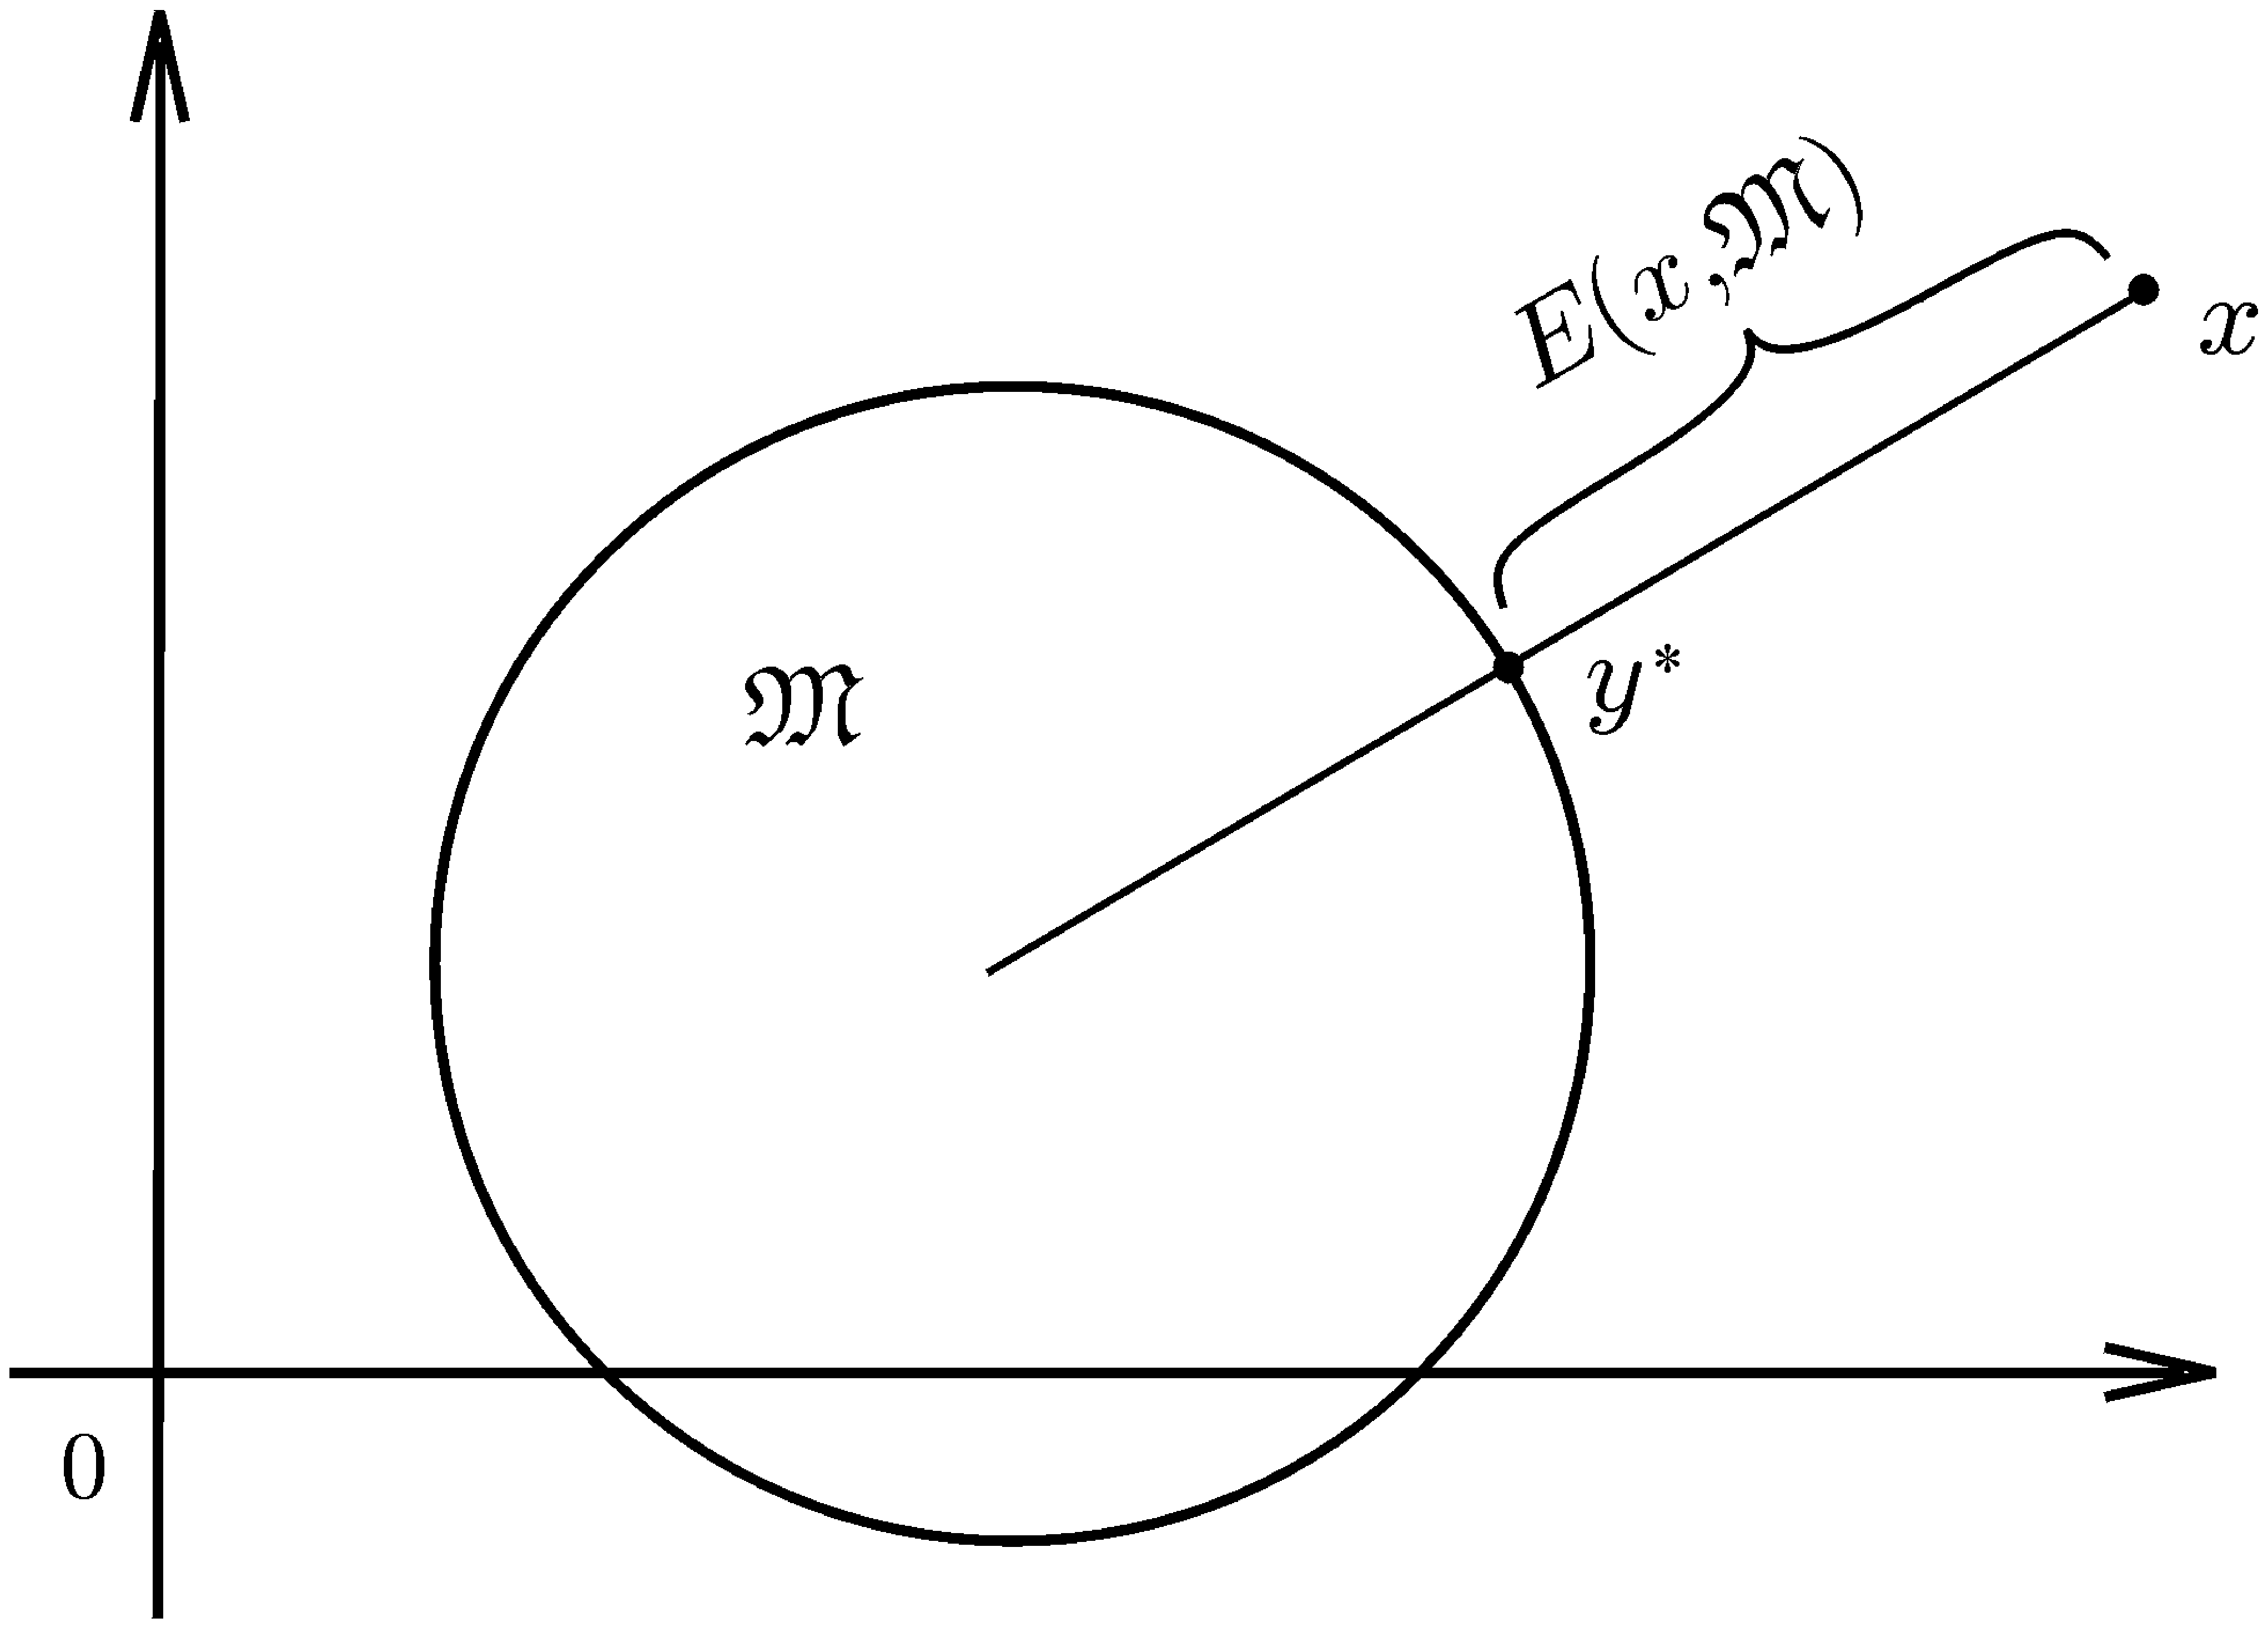
\includegraphics[width=0.5\textwidth]{pict/pict01-1.eps}
\end{center}
 \bigskip
 \refstepcounter{ris}\label{r1-1}

 \centerline{Рис.~\theris}
 \bigskip
\end{figure}

%%%%%%%%%%%%%%%%%%%%%%%%%%%%%%%%%%%%%%%%%%%%%%%%%%%%%%%%%%


Наилучшее приближение и наилучший элемент обладают и другими
неприятными особенностями. Поясним на
примере.

\begin{Example}
$X=C[a,b],$~ $-\infty < a < b < +\infty$ {(функция $f\in
C[a,b]$,} {если она непрерывна на $[a,b]$)},
{$\|f\|_C=\max\limits_{x\in[a,b]}|f(x)|$,}
$\ro(f,g)=\|f-g\|_C$. В качестве $\G M$ возьмем $\G M=\{c \}$
{--} множество констант $c \in \bR${, точнее, множество}
{постоянных функций}. Тогда, очевидно, {для любой} $ f
\in C[a,b]$ существует единственный наилучший элемент $c^* \in
\G M$, {
$$
c^* = \frac{\max\limits_{x\in[a,b]}{f(x)}+\min\limits_{x\in[a,b]} {f(x)}}{2}
$$
}
(см. рис.~\ref{r1-2}).
\end{Example}

%%%%%%%%%%%%%%%%%%%%%%%%%%%%%%%%%%%%%%%%%%%%%%%%%%%%%%
%\vspace{5mm}

\begin{figure}[ht]
\begin{center}
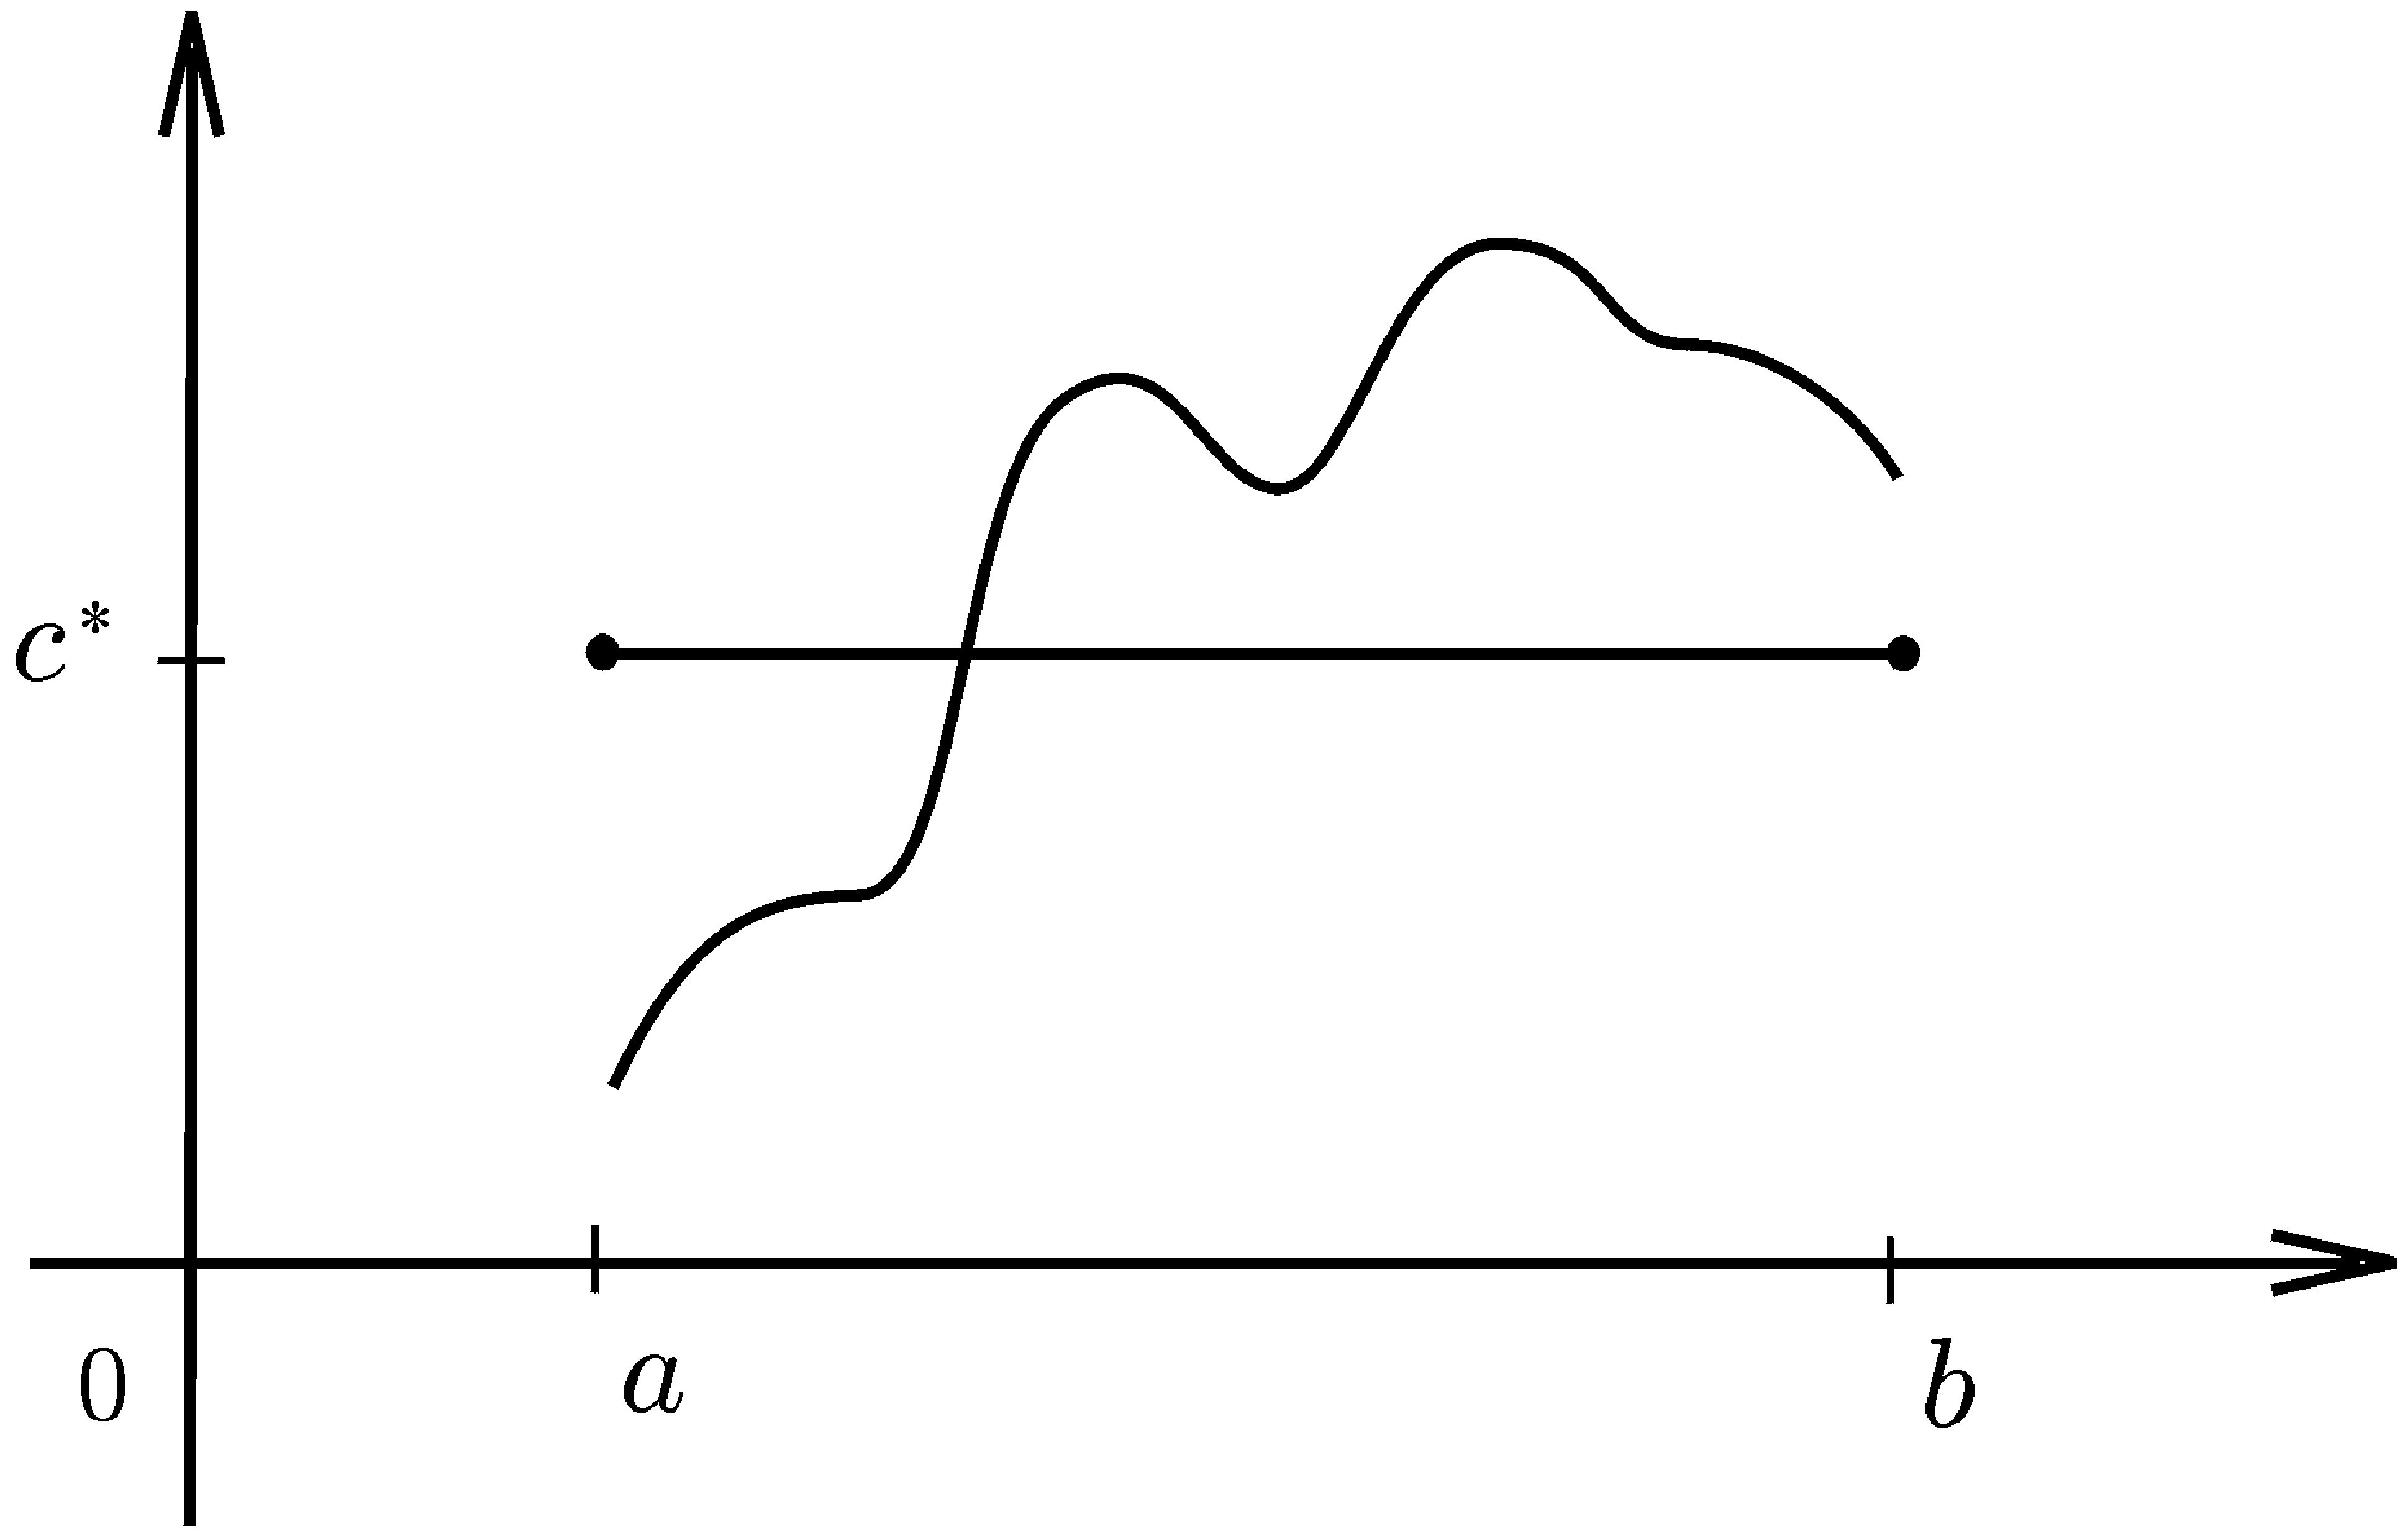
\includegraphics[width=0.5\textwidth]{pict/pict01-2.eps}
\end{center}
 \bigskip
 \refstepcounter{ris}\label{r1-2}

 \centerline{Рис.~\theris}
 \bigskip
\end{figure}

% \bigskip
% \begin{picture}(70,170)
% \put(100,160){\special{em: graph pict01-2.eps}}
% \end{picture}
% \refstepcounter{ris}\label{r1-2}

% \centerline{Рис.~\theris}
% \bigskip

%%%%%%%%%%%%%%%%%%%%%%%%%%%%%%%%%%%%%%%%%%%%%%%%%%%%%%%%%%



Итак, возникает оператор {наилучшего приближения} $A${,}
любой функции $f \in C[a,b]$ ставящий в соответствие
наилучший элемент $c^* \in \G M$: $A(f)=c^*(f).$ Этот оператор не является линейным.
Действительно, если мы возьмем $f_1$ и $f_2$ как на рис.~\ref{r1-3}, то
$c^*(f_1)=c^*(f_2)=c^*(f_1+f_2)=h/2,$ т.\,е. $A(f_1+f_2)\ne A(f_1)+A(f_2).$

%%%%%%%%%%%%%%%%%%%%%%%%%%%%%%%%%%%%%%%%%%%%%%%%%%%%%%
%\vspace{5mm}

\begin{figure}[ht]
\begin{center}
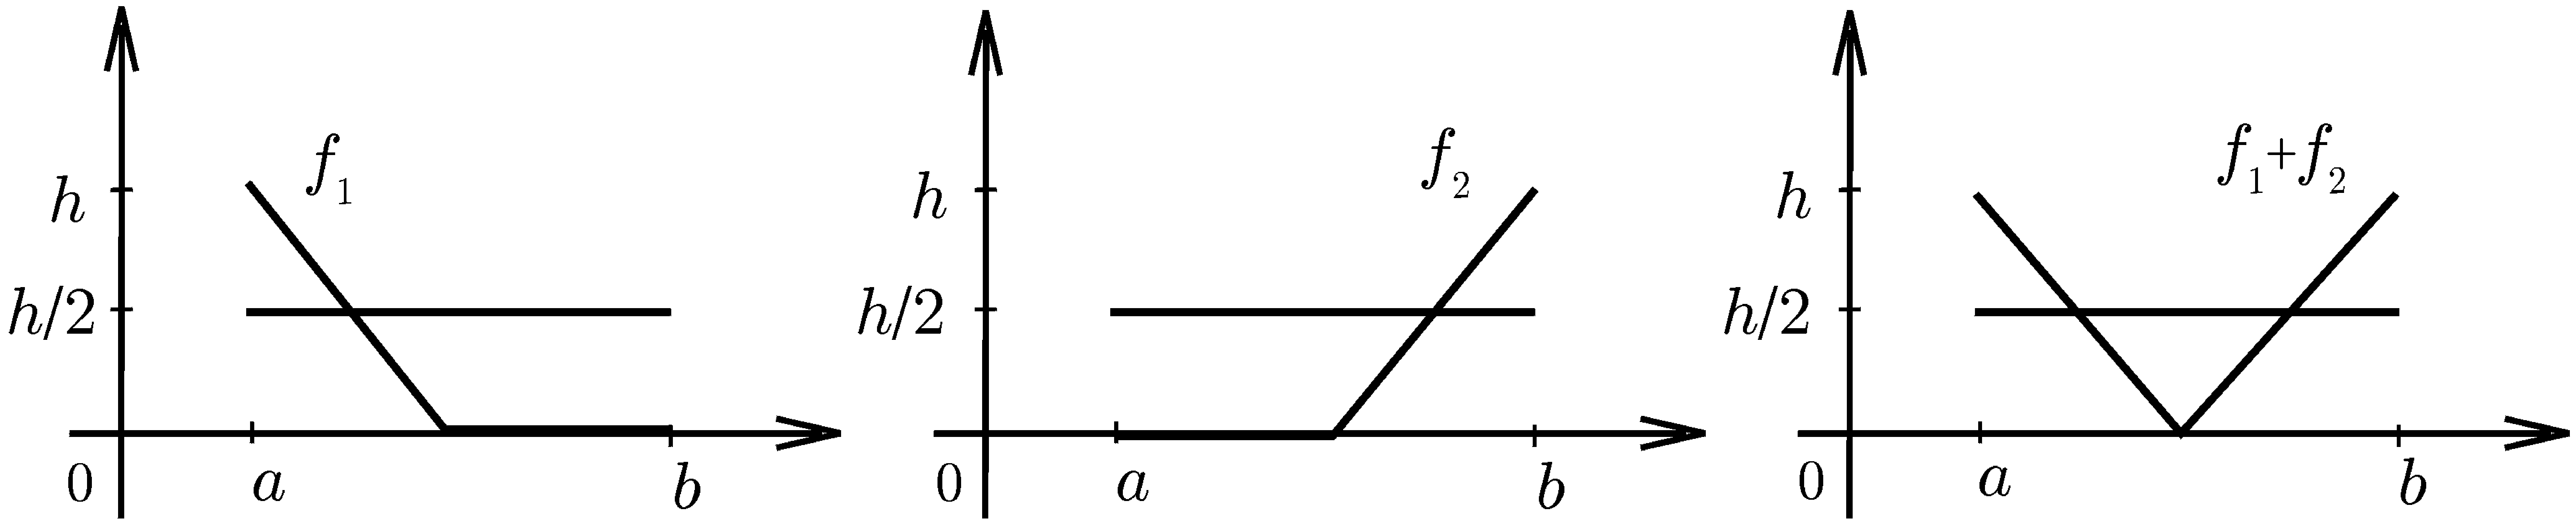
\includegraphics[width=0.9\textwidth]{pict/pict01-3.eps}
\end{center}
 \bigskip
 \refstepcounter{ris}\label{r1-3}

 \centerline{Рис.~\theris}
 \bigskip
\end{figure}



% \bigskip
% \begin{picture}(0,120)
% \put(-10,120){\special{em: graph pict01-3.pcx}}
% \end{picture}
%\centerline{рис. 3} \vspace{5mm}
% \refstepcounter{ris}\label{r1-3}

% \centerline{Рис.~\theris}
% \bigskip

Итак, в некоторых функциональных пространствах {оператор наилучшего} {приближения}
$A$ не является линейным, значит,
{найти} $E{(x)}$ и $y^*{(x)}$ {может} {оказаться трудной задачей. Поэтому рассматривают и
более простые методы} {приближения. В частности, различные линейные методы.}

\section{Линейная задача теории приближения}

Пусть $X=C[a,b]=C$ и $\Cal L$ -- некоторое {подпространство} из $C$ и пусть $A$~--
линейный оператор из $C$ в $C$ и {$Af \in \Cal L$} для любой функции $f \in C[a,b].$
Будем говорить в этом случае, что в $C$ задан линейный метод $A$ приближения элементов
{из} $C$ посредством подпространства $\Cal L$. {Для $f$ в качестве приближающего
выступает элемент $Af$.}

Интерполирование -- первый классический метод линейного приближения.

\section{Лагранжево интерполирование}

Пусть функция $f \in C[a,b]$ (пока можно считать, что значения $f(x) \in \bC$~--
множеству комплексных чисел).

Возьмем на $[a,b]$ {различные точки} $x_k\ (k=0,1,\ldots,n)$. Можно считать, что
$a \le x_0 <x_1< \cdots <x_n \le b.$ Точки $\{x_k\}$ будут называться {\it узлами
интерполяции}.

Задача состоит в том, чтобы для узлов $\{x_k\}$ и для любого набора {чисел} $\{y_k\}\
(k=0,1,\dots ,n)$ построить многочлен $p_n \in \mathcal{P}_n,$
\[
  p_n(x)=a_0+a_1x+\cdots +a_n x^n,
\]
такой, что $p_n(x_k)=y_k$\  $(k=0,1,\dots ,n).$

Возникают вопросы:
\smallskip
1) Всегда ли задача разрешима?
\smallskip
2) Сколько имеется решений?
\smallskip

Здесь для определения коэффициентов $a_i\ (i=0,1,\dots,n)$ получается система линейных
уравнений с определителем Вандермонда, не равным $0.$ Следовательно, для любых $x_k$ и
любых $y_k$ имеется единственное решение. Поэтому достаточно {выписать} решение в
явном виде. {С этой целью для} любого $k=0,1,\dots,n$ построим фундаментальный
многочлен {$l_k(x)$} лагранжевой интерполяции, соответствующий $k$-му узлу, -- это
многочлен степени $n$, обладающий свойствами: $l_k(x_i)=\delta_{i,k}$, где
$\delta_{i,k}$ -- символ Кронекера, $\delta_{k,k}=1, \ \delta_{i,k}=0$ при $i \ne k$.

Очевидно,
\[
  l_k(x)=\frac{(x-x_0)(x-x_1)\cdots (x-x_{k-1})(x-x_{k+1})\cdots (x-x_n)}
         {(x_k-x_0)(x_k-x_1)\cdots (x_k-x_{k-1})(x_k-x_{k+1})\cdots (x_k-x_n)}.
\]
Обозначим $\omega(x)=\prod_{k=0}^n(x-x_k).$
Тогда
$$
\omega'(x_k)=
      (x_k-x_0)(x_k-x_1)\cdots (x_k-x_{k-1})(x_k-x_{k+1})\cdots (x_k-x_n)
$$
и, следовательно,
\[
 l_k(x)=\frac{\omega(x)}{(x-x_k)\omega'(x_k)}.
\]
Ясно, что
\[
 p_n(x)=p_{n}(x,\{y_k\},\{x_k\})=
 %\sum_{k=0}^n y_k
 %\frac{\omega(x)}{(x-x_k)\omega'(x_k)}=
 \sum\limits_{k=0}^n y_k l_k(x)
\]
-- искомый многочлен. Интерполяционный многочлен
рассматриваемой задачи, записанный в этой форме, называется {\it
интерполяционным многочленом Лагранжа}.

Пусть теперь $f \in C[a,b],$~ $\{x_k\}$~-- узлы интерполяции, а $y_k=f(x_k)$\
$(k=0,1,\dots ,n).$ Тогда для любой функции $f \in C[a,b]$ и любых узлов
{интерполяции} $\{x_k\}$\  $(k=0,1,\dots ,n)$ существует единственный многочлен
$$
p_n(x,f)=p_n(x,f,\{x_k\})=\sum\limits_{k=0}^n f(x_k) l_k(x)
$$
степени не выше $n$, который удовлетворяет условиям
\[
 p_n(x_k,f)=f(x_k)\qquad (k=0,1,\dots ,n).
\]
Таким образом, возникает {оператор} $P_n:\ f \longmapsto p_n(x,f)$ {из} $C{[a,
b]}$ в $C{[a,b]}$. {Отметим} простейшие свойства {этого оператора.}

1) {Если} $f \in \Cal P_n$, то для любых узлов $\{x_k\}$
имеем $p_n(x,f)\equiv f(x),$ т.\,е. $P_{n}(f)=f.$

2) $f \to P_n(\cdot,f)$
~-- линейный (т.\,е. однородный, аддитивный) ограниченный оператор:
$$
  P_n(c_1f_1+c_2f_2) \equiv c_1P_n(f_1)+c_2P_n(f_2),\qquad
  f_i\in C[a,b],\qquad c_i\in \bR\qquad (i=1,2),
$$
и для любой функции
$f\in C[a,b]$
$$
  \|p_n(\cdot,f)\|_C \le L_n\|f\|_C,\ \ \mbox{где}\ \
  L_n=\|P_n\|_C^C<\infty.
$$

Более того,
$$
|p_n(x,f)| \le L_n(x)\|f\|_C.
$$
Здесь $L_n(x)=\sum{|l_k(x)|},$~ $L_n =
\|L_n(x)\|_C$. Оба неравенства вытекают из формулы для $p_n(x, f) = p_n(x,f,\{x_k\})$. В
пространстве $C[a,b]$ они являются точными.

{Действительно, определим
при фиксированном $\xi \in [a,b]$ функцию $f_\xi(x)$ так,
чтобы она удовлетворяла условиям}

{а) $f_\xi(x)=\sign{l_k(\xi)}$ при $x=x_k\  ( k=0,1,\ldots,n)$,}

{б) $|f_\xi(x)| \le 1$ при $x \in [a,b]$,}

{в) $f_\xi(x)$ непрерывна по $x$ на $[a,b]$.}

{Тогда будем иметь
$$
\|f_\xi\|_C=1,
\qquad  p_n(x, f_\xi) = \sum\limits^n_{k=0}{f_\xi(x_k)l_k(x)}
$$
и, в частности,
$$
  p_n(\xi, f_\xi) = \sum\limits^n_{k=0}{|l_k(\xi)|} =
  L_n(\xi)\|f_\xi\|_C,
$$
а выбирая здесь в качестве $\xi$ точку $x^*$ максимума на $[a,b]$ функции $L_n(x)$,
получим
$$
  p_n(x^*,f_{x^*}(\cdot)) = L_n\|f_{x^*}\|_C
$$
и, следовательно,
$$
  \|p_n(x,f_{x^*}(\cdot))\|_C = L_n\|f_{x^*}\|_C.
$$}

{Таким образом, константа $L_n$ есть норма оператора $P_n\colon f \longmapsto p_n(x,f):$
$$
  \|P_n\|_{C \to C} = L_n.
$$
А для любого фиксированного $x \in [a,b]$ величина $L_n(x)$ является нормой функционала
$P_x(f)=p_n(x,f)$ в $C[a,b]$:
$$
\|P_x(f)\| = L_n(x),
$$
так как
$$
|P_x(f)| \le L_n(x)\|f\|_C\qquad \forall\ f \in C[a,b]
$$
и
$$
|P_x(f_x(\cdot))|=L_n(x)\|f_x\|_C.
$$}

{Константа $L_n$ называется \textit{константой Лебега}, а $L_n(x)$ --
\textit{функцией Лебега} линейного метода $p_n(x, f, \{x_k\})$ приближения функций $f$ из
$C[a,b]$ интерполяционными многочленами Лагранжа. Ясно, как эти понятия распространяются
на другие линейные методы приближения.}

{Метод интерполирования тем <<лучше>>, чем меньше его норма, т.\,е. константа Лебега. При
$n$ фиксированном $L_n$ зависит от узлов интерполирования $\{x_k\}$. Если $[a,b]=[-1,1]$,
то можно узлы выбрать так, что $L_n=\dfrac{2}{\pi}\ln{n} + O(1)$~ $(n \to +\infty)$, а
именно, в качестве узлов интерполяции нужно взять нули многочлена Чебышева
$$
T_{n+1}(x)=\cos({(n+1)}\arccos{x}).
$$}

3) Тождества Коши.

Из свойства 1) и формулы для интерполяционного многочлена {при $f(x)\equiv 1$}
получаем {тождество}
\[ \sum\limits_{k=0}^n l_k(x) \equiv 1, \]
{а при} $f(x)=(x-u)^j$~ $(j=1,\dots ,n;\ u\in \mathbb C)$ {-- тождества}
$$
(x-u)^j\equiv \sum\limits_{k=0}^n (x_k-u)^j l_k(x) \qquad (j=1,2,\ldots,n),
$$
{откуда при} $u=x$ следует, {что}
\begin{equation}\label{f1-1}
\sum\limits_{k=0}^n (x_k-x)^j l_k(x)\equiv 0\qquad (j=1,\ldots ,n).
\end{equation}
Эти тождества при $\{x_n\}\subset [a,b]$ справедливы для
всех $x\in \mathbb C.$

\section{Оценка погрешности интерполяционной \\ формулы
Лагранжа. Неравенства Лебега}

Пусть $\{x_k\}_{k=0}^n$~-- узлы интерполяции, $f \in C[a,b],$ $p_n(x,f)$ --
соответствующий интерполяционный многочлен Лагранжа. Можно написать
\[
  f(x)=p_n(x,f)+R_n(x,f),
\]
где $R_n(x,f)$~-- остаточный член. Очевидно, в узлах интерполяции $R_n(x_k,f)=0$~
$(k=0,\dots ,n).$ Требуется оценить $R_n(x,f)$ для любого фиксированного $x \in [a,b],$
а также оценить $\|R_n(\cdot ,f)\|_{C[a,b]}.$

Оказывается, для оценок остаточного члена лагранжевой интерполяции {достаточно} знать
$L_n(x),$ $L_n$ {и} $E(f ,\Cal P_n)_C=\inf\limits_{q \in \Cal P_n}\|f-q\|_{{C}}.$
Именно, имеют место неравенства Лебега
\[  |R_n(x,f)|\le (L_n(x)+1)E(f ,\Cal P_n)_C,             \]
\[  \|R_n(\cdot ,f)\|_{{C}} \le (L_n+1)E(f ,\Cal P_n)_C.             \]
Для доказательства воспользуемся тем, что $P_n(x,f)$~-- линейный оператор, и
$P_n(x,q)=q(x)$ для любого $q \in \Cal P_n$ ({аналогичные неравенства} Лебега
{возникают} и {для} более {общих линейных методов, сохраняющих элементы $\Cal
P_n$ на месте}). Имеем
\begin{multline*}
  |R_n(x,f)|=|f(x)-p_n(x,f)|=|f(x)-q(x)-p_n(x,f-q)|\le  \\
  \le |f(x)-q(x)|+L_n(x)\|f-q\| \le
      (L_n(x)+1)\|f-q\|_{{C}}, \qquad q \in \Cal P_n.
\end{multline*}
Значит, если в качестве $q$
возьмем наилучший элемент для $f$
в $\Cal P_n,$
то получим
\[  |R_n(x,f)|\le (L_n(x)+1)E(f ,\Cal P_n)_C,\qquad x\in [a,b],   \]
откуда следует, что
\[  \|R_n(\cdot ,f)\|_{{C}} \le (L_n+1)E(f ,\Cal P_n)_C.             \]

\section{Остаточный член в форме Коши\\
 для интерполяционной формулы Лагранжа}

%%%%%%%%%%%%%%%%%%%%%%%%%%%%%%%%%%%%%%%%%%%%%%%%%%%%%%%%%
{Функция $f \in C^{(n+1)}[a,b],$ если $f$ непрерывна на $[a,b]$ вместе с производными
до} {порядка $n+1$ включительно.}

\begin{teo}\label{t1-1}
Пусть $f \in C^{(n+1)}[a,b].$ Тогда для любого $x \in [a,b]$ существует {точка} $\xi
\in (a,b)$ {такая}, что
\[
  R_n(x,f)=\frac{f^{(n+1)}(\xi)}{(n+1)!}\omega (x)
\]
$(${здесь $\xi=\xi(x,f,\{x_k\})$},~ $n+1$~-- число узлов
интерполяции$).$
\end{teo}

\begin{proof}
{Доказываемая формула, очевидно, верна для $x=x_k$}
{$(k=0,\dots ,n)$} ($\xi$ может любой точкой). Зафиксируем {$x \in [a,b],$~ $x \ne x_k,$}
и рассмотрим вспомогательную функцию
\[
  F(t)=f(t)-p_n(t)-K\omega (t),
\]
где {$p_n(t)=p_n(t,f,\{x_k\}),$~ $K=R_n(x,f)/ \omega (x), \ \omega(x) \ne 0.$} Заметим,
что $F(t)$ при $t=x_k$ равна нулю $(k=0,\dots ,n)$ и $F(x)=0$ по выбору $K.$ Следовательно, функция
{$F(t)$} имеет нули в ${n+2}$ различных точках. Применим обобщенную теорему Ролля, из
которой следует, что найдется точка $\xi \in (a,b)$ такая, что $F^{(n+1)}(\xi)=0$.
{Но} $F^{(n+1)}(\xi)=f^{(n+1)}(\xi)-K\cdot (n+1)!,$ значит,
$K=f^{(n+1)}(\xi)/(n+1)!,$ откуда {для} $R_n(x,f)=K\omega(x)$ {получаем}
\[
  R_n(x,f)=\frac{f^{(n+1)}(\xi)}{(n+1)!}\omega (x)
\]
и теорема доказана.
\end{proof}

\begin{Remark}[геометрическое]
{Остаточный} член не обязан менять знак в узлах {интерполяции вслед за
$\omega(x).$} Графики $f(x)$ и $p_n(x,f)$ могут соприкасаться, как показано на
рис.~\ref{r1-4}.
\end{Remark}

%%%%%%%%%%%%%%%%%%%%%%%%%%%%%%%%%%%%%%%%%%%%%%%%%%%%%%
%\vspace{5mm}

\begin{figure}[ht]
\begin{center}
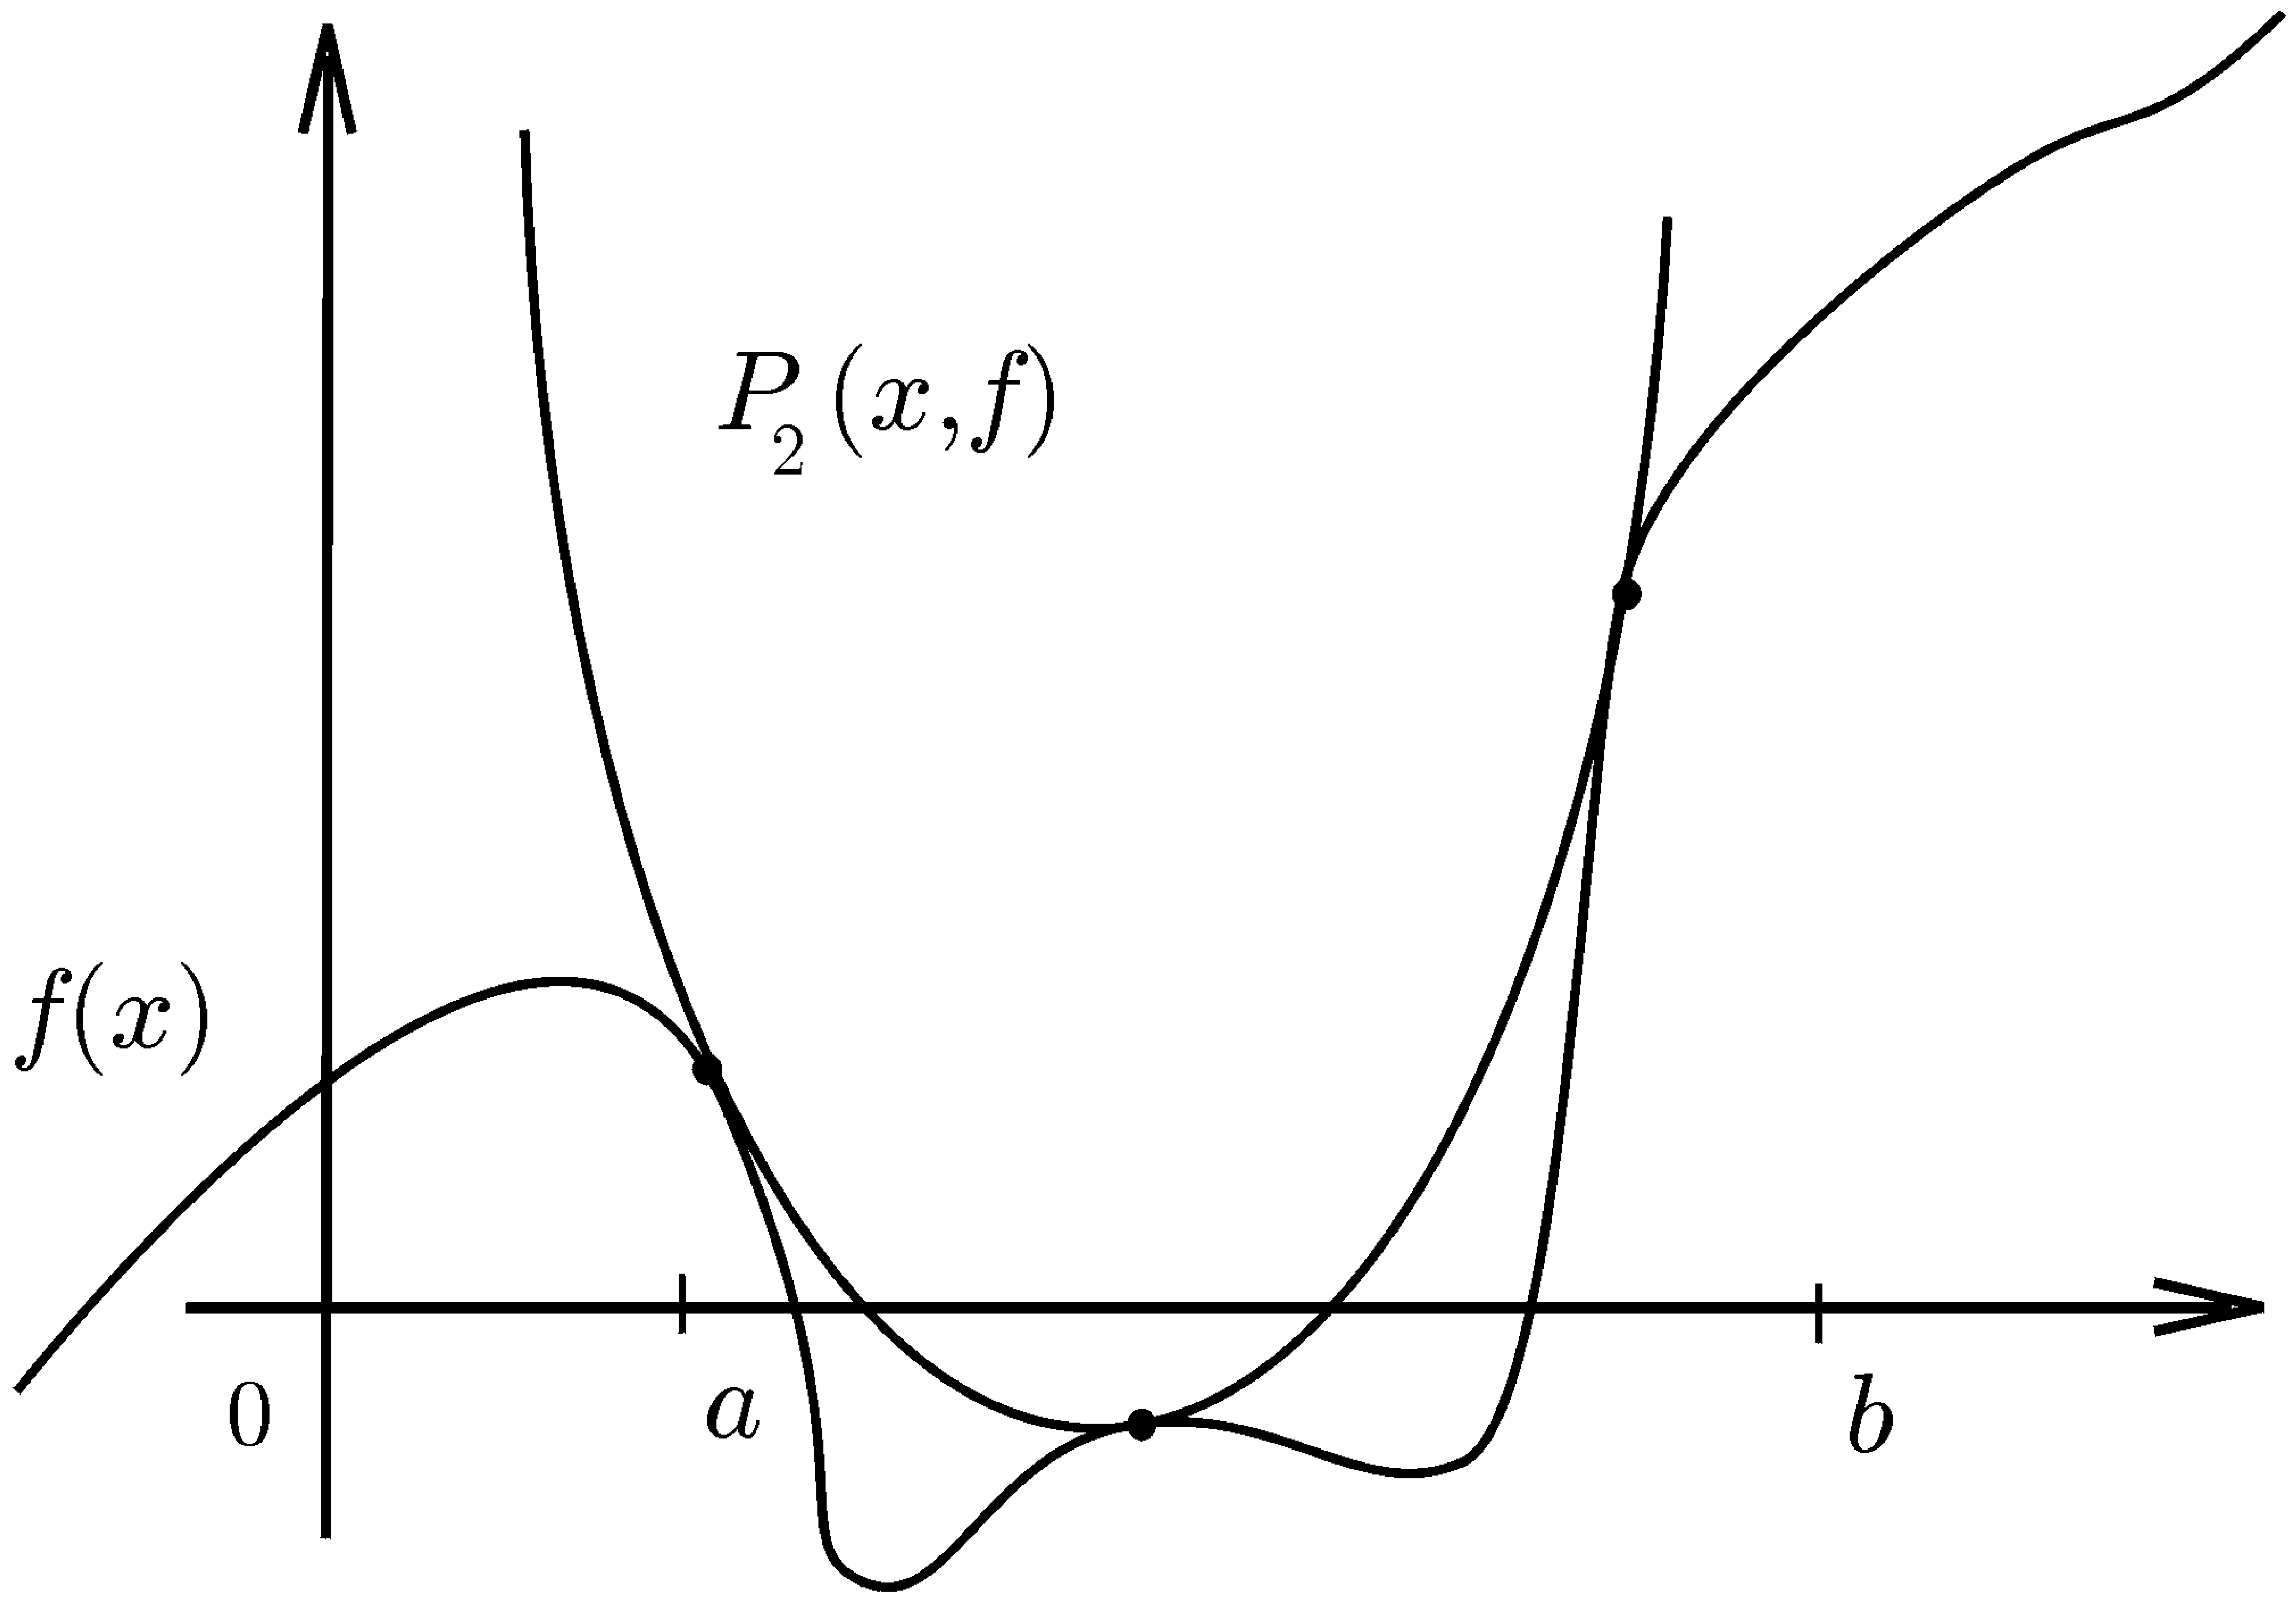
\includegraphics[width=0.5\textwidth]{pict/pict01-4.eps}
\end{center}
 \bigskip
 \refstepcounter{ris}\label{r1-4}

 \centerline{Рис.~\theris}
 \bigskip
\end{figure}



% \bigskip
% \begin{picture}(70,190)
% \put(90,190){\special{em: graph pict01-4.pcx}}
% \end{picture}
%\hbox to 0.5cm {}{\special{em:graph pict4.pcx}}
%\vspace{6cm}

% \refstepcounter{ris}\label{r1-4}

% \centerline{Рис.~\theris}
% \bigskip

%%%%%%%%%%%%%%%%%%%%%%%%%%%%%%%%%%%%%%%%%%%%%%%%%%%%%%%%%%
%\noindent \hskip3.0cm {\rm рис. 4}
%\bigskip



Но есть достаточное условие того, что остаточный член меняет знак в узлах. Как видно из
формулы для остаточного члена интерполяции в форме Коши, {\it если} $f^{(n+1)}(x)$
{\it сохраняет знак}, {\it то} $R_n(x,f)$ {\it меняет знак в узлах интерполяции и только в них}.

Обозначим $M_{n+1}(f)=\max\limits_{x \in [a,b]}f^{(n+1)}(x).$

\begin{Corollary}
\[
 \|R_n(\cdot ,f) \|_C \le \frac{M_{n+1}(f)}{(n+1)!}\|\omega(\cdot ) \|_C .
\]
\end{Corollary}

\begin{task}
При каком выборе узлов интерполяции величина $\|\omega(\cdot ) \|_C$
наименьшая?
\end{task}

 Оказывается {это будет,} когда $\omega$~-- многочлен
Чебышева\footnote{{Свойства} многочлена Чебышева приводятся в лекции 2.}
{$\widetilde{T}_{n+1}(x,I)$ $(I=[a,b]).$}
{Действительно, } $\omega(x)=x^{n+1} +a_{n}x^n+ \dots +a_0.$ Так {что}
\[
  \inf \|\omega(\cdot)\|_{C[a,b]}=\|\widetilde{T}_{n+1}(\cdot{, I})\|_{C[a,b]},
\]
где $\widetilde{T}_{n+1}{(\cdot, I)}$~-- многочлен Чебышева
на $[a,b],$ т.\,е. наименее
уклоняющийся на $[a,b]$ от нуля многочлен {степени $n+1$} со
старшим коэффициентом 1. В частности, $\widetilde{T}_{n+1}(x,[-1,1])=
\dfrac1{2^n}\cos(n+1)\arccos x.$


\section{Теорема Хаара об интерполяции в $\mathbb R^N$}

Мы рассматривали {задачу} интерполяции на {$D=[a,b] \subset
\bR^1$} т.\,е. в одномерном случае. Пусть теперь множество {$D \subset \bR^N,\ N\ge 2.$}

{{В о п р о с ы}. \hspace{1em}}

Имеет ли смысл задача {интерполяции} в многомерном случае?

Существуют ли действительные функции {$f_0(x),f_1(x),\dots,f_n(x),$~ $x \in
\overline{D} \subset \bR^N,$} ({\it интерполяционные системы на} $D$), {линейными
комбинациями которых} можно интерполировать {любой набор чисел $\{y_k\}_{k=0}^n$ в} любых
{несовпадающих узлах} $\{x_k\}_{k=0}^n \in D?$

Легко убедиться, что интерполяционные системы, состоящие из
разрывных функций, существуют на любом множестве мощности континуум. Для
этого достаточно рассмотреть взаимно однозначное
отображение отрезка на множество и взять порожденные им функции,
соответствующие рассмотренной нами на отрезке
интерполяционной системе $1,x,x^2,\dots ,x^n.$

Далее будет показано, что задача интерполяции многочленами разрешима
в комплексной области. А ответ на вопрос об $\bR^N$ дает следующая теорема.

\begin{teo}[А.\,Хаар]
Если $N>1$ и множество $D\subset \mathbb R^N$ имеет
внутренние точки, т.\,е. {$\inter {D} \ne \varnothing,$} и если $n \ne 0,$ то {в
$D$ не существует} непрерывных действительных интерполяционных систем {$($т.\,е.
систем, которыми можно интерполировать} при любом выборе узлов $\{x_k\}^{n}_{k=0}$
любой набор чисел $\{ y_k\}_{k=0}^n).$
\end{teo}

\begin{proof}
Возьмем внутреннюю точку и ее некоторую
окрестность $\Delta \subset D,$
и пусть {$\{x_k\}_{k=0}^n \subset \Delta.$}

%%%%%%%%%%%%%%%%%%%%%%%%%%%%%%%%%%%%%%%%%%%%%%%%%%%%%%

\begin{figure}[ht]
\begin{center}
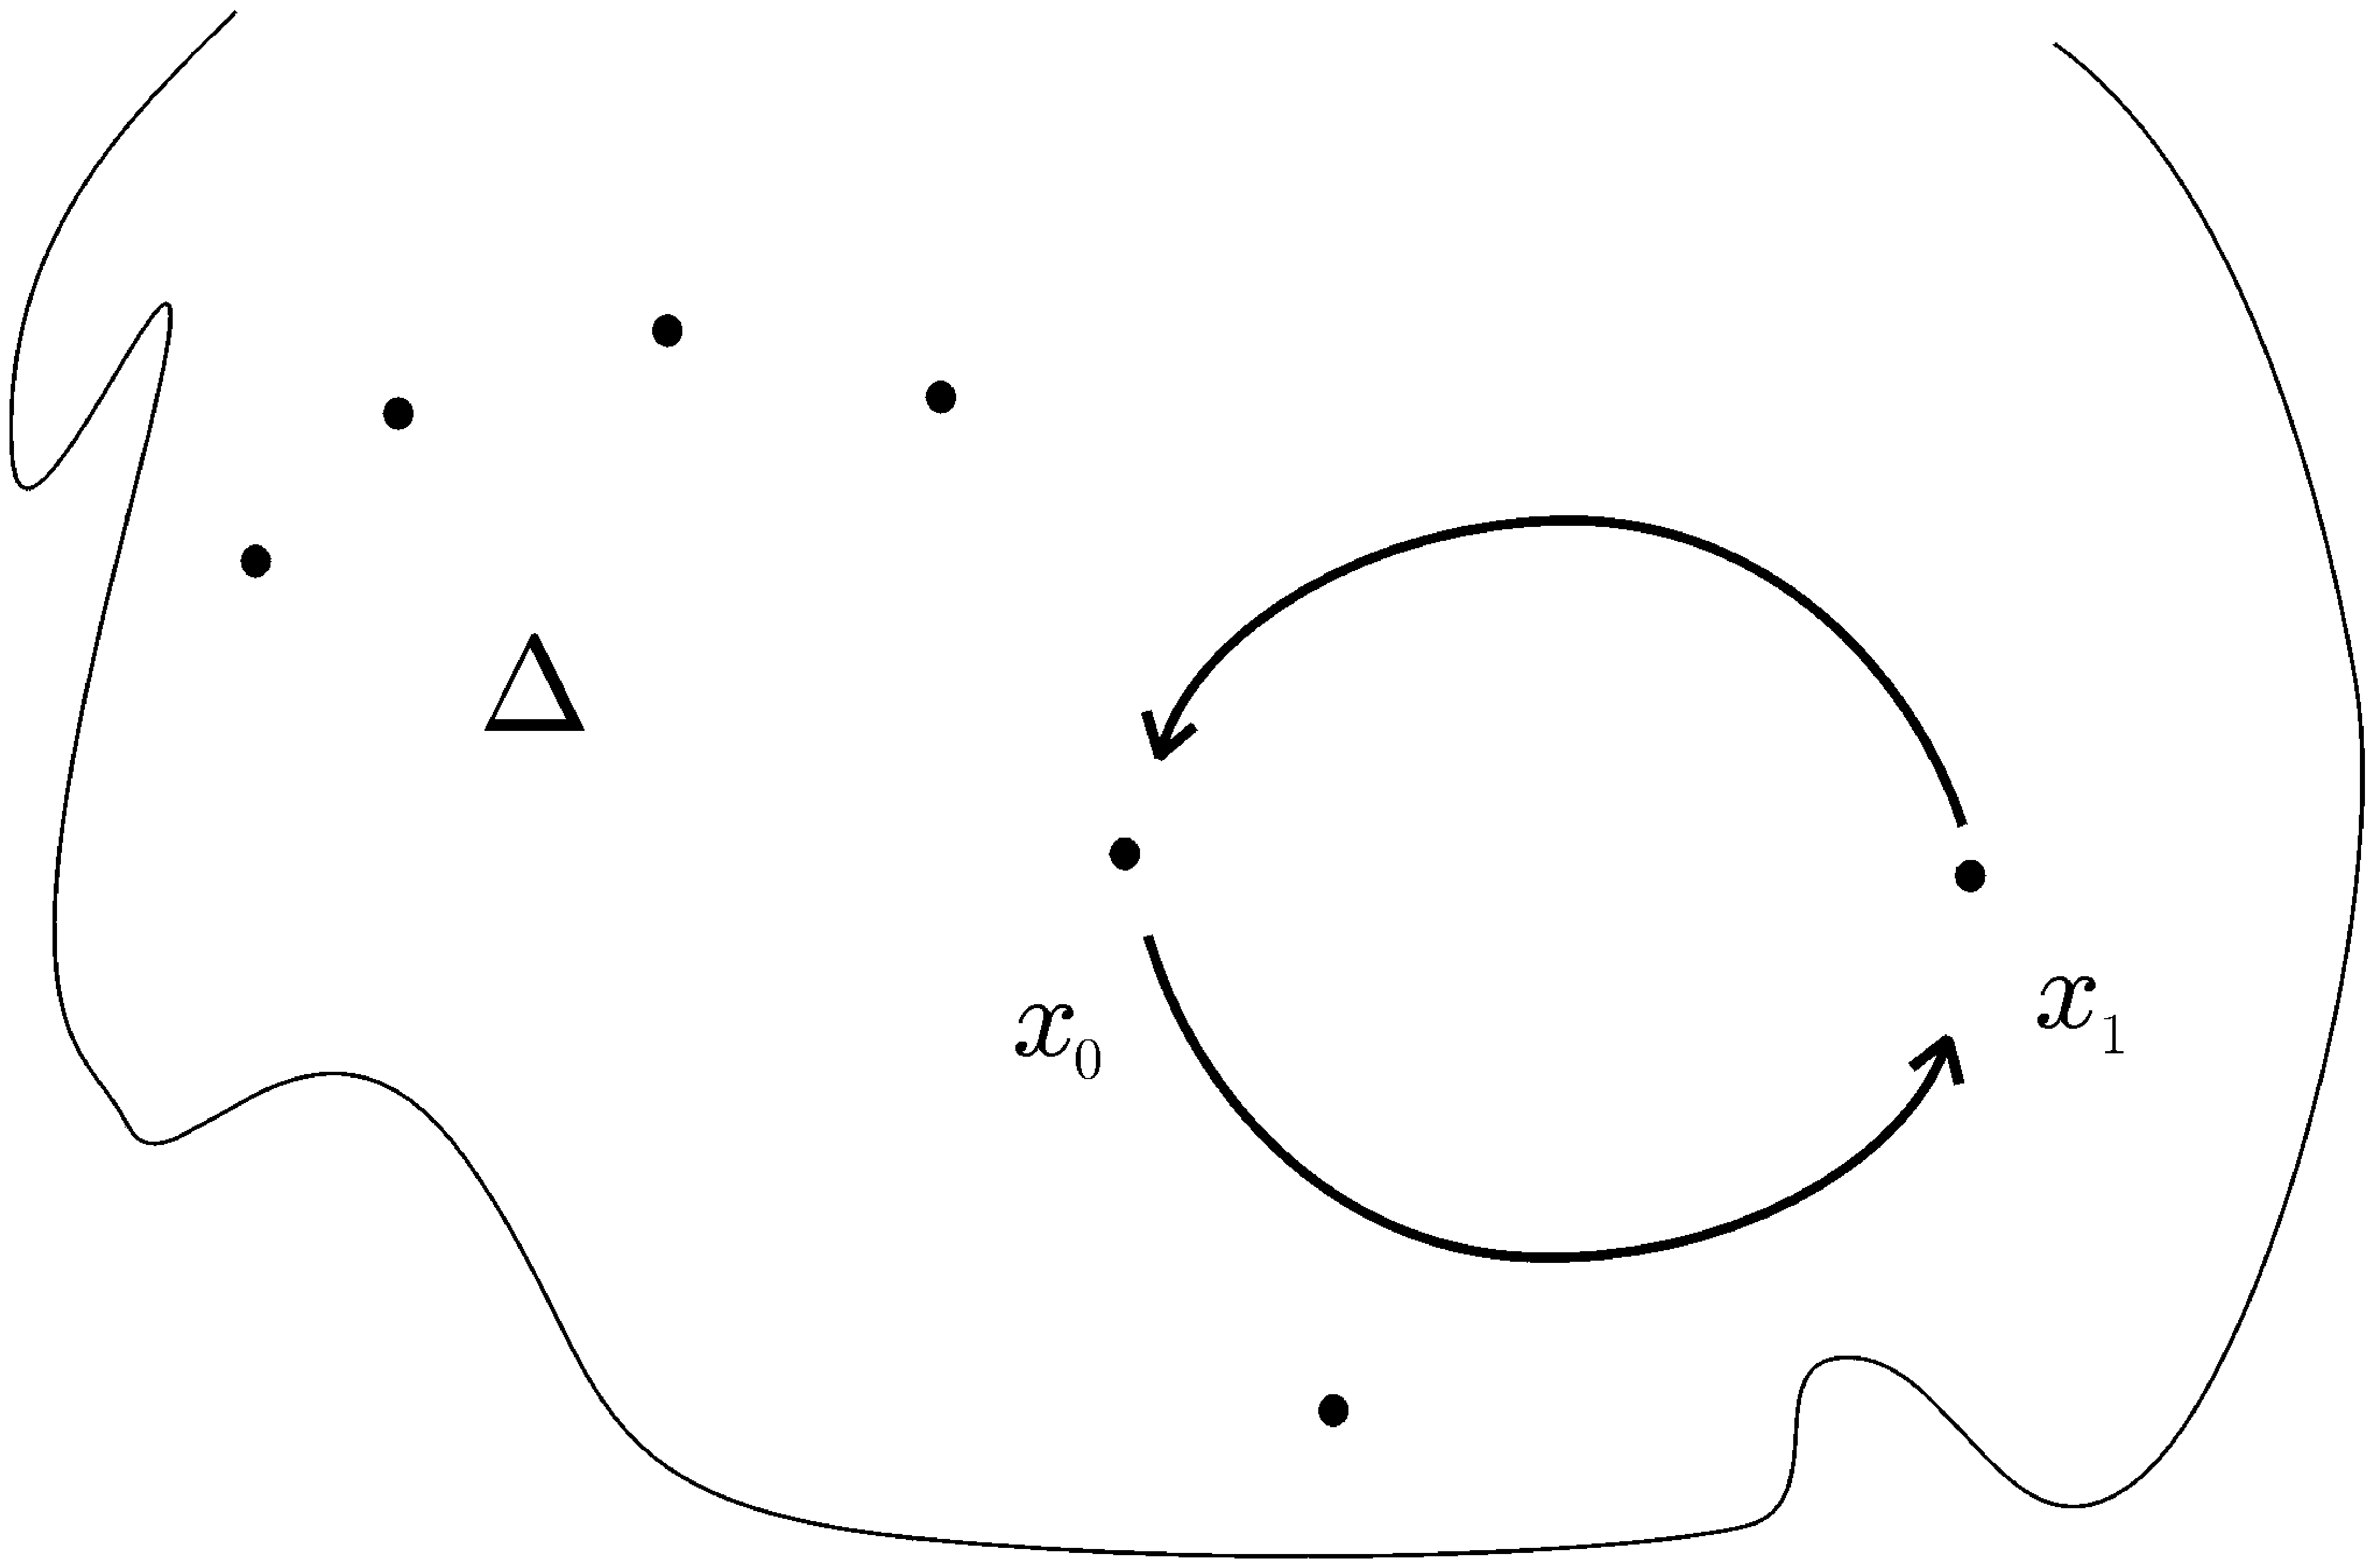
\includegraphics[width=0.5\textwidth]{pict/pict01-5.eps}
\end{center}
 \bigskip
 \refstepcounter{ris}\label{r1-5}

 \centerline{Рис.~\theris}
 \bigskip
\end{figure}




\noindent Если система {$\{f_k\}$~ $(k=0,\ldots,n)$} интерполяционная, то система
уравнений
\[
  \sum\limits^{n}_{k=0}c_k f_k(x_i)=y_i\qquad ({i}=0,\dots ,n),
\]
разрешима для любых {наборов чисел $\{y_k\}$}. {Отсюда следует, что} $\det
(f_k(x_i)) \ne 0$ {для любых $\{x_k\} \subset \Delta$.} По условию функции
$f_k$ непрерывны, следовательно, определитель непрерывен как функция от точек
$\{x_i\}$ в области $\Delta.$ Теперь все точки $x_k$ в $\Delta,$ кроме двух, например
$x_0$ и $x_1$, оставим на месте, а $x_0$ и $x_1$ будем непрерывно переводить друг в
друга {(см. рис.~\ref{r1-5})} {так, что при движении все $n+1$ точки
остаются различными и принадлежат $\Delta$.} Определитель будет непрерывно меняться,
{оставаясь вещественным,} и переменит знак (поменяются местами две строки
определителя). Следовательно, { при каком-то} {промежуточном наборе точек он
обращался в нуль. Это противоречие доказывает } {теорему. }
\end{proof}

\begin{Remark}
Непрерывные действительные интерполяционные
системы не существуют не только на множествах с непустой
внутренностью, но даже на континууме
с точкой ветвления.
\end{Remark}
Действительно, поменяем точки $x_0$ и $x_1$ {местами, перемещая их непрерывно,} как
показано на рис.~\ref{r1-6}, знак определителя изменится, следовательно, он обращался в
нуль, чего  не {должно} быть для непрерывных интерполяционных систем.

%%%%%%%%%%%%%%%%%%%%%%%%%%%%%%%%%%%%%%%%%%%%%%%%%%%%%%
 \bigskip
\begin{figure}[h]
\begin{center}
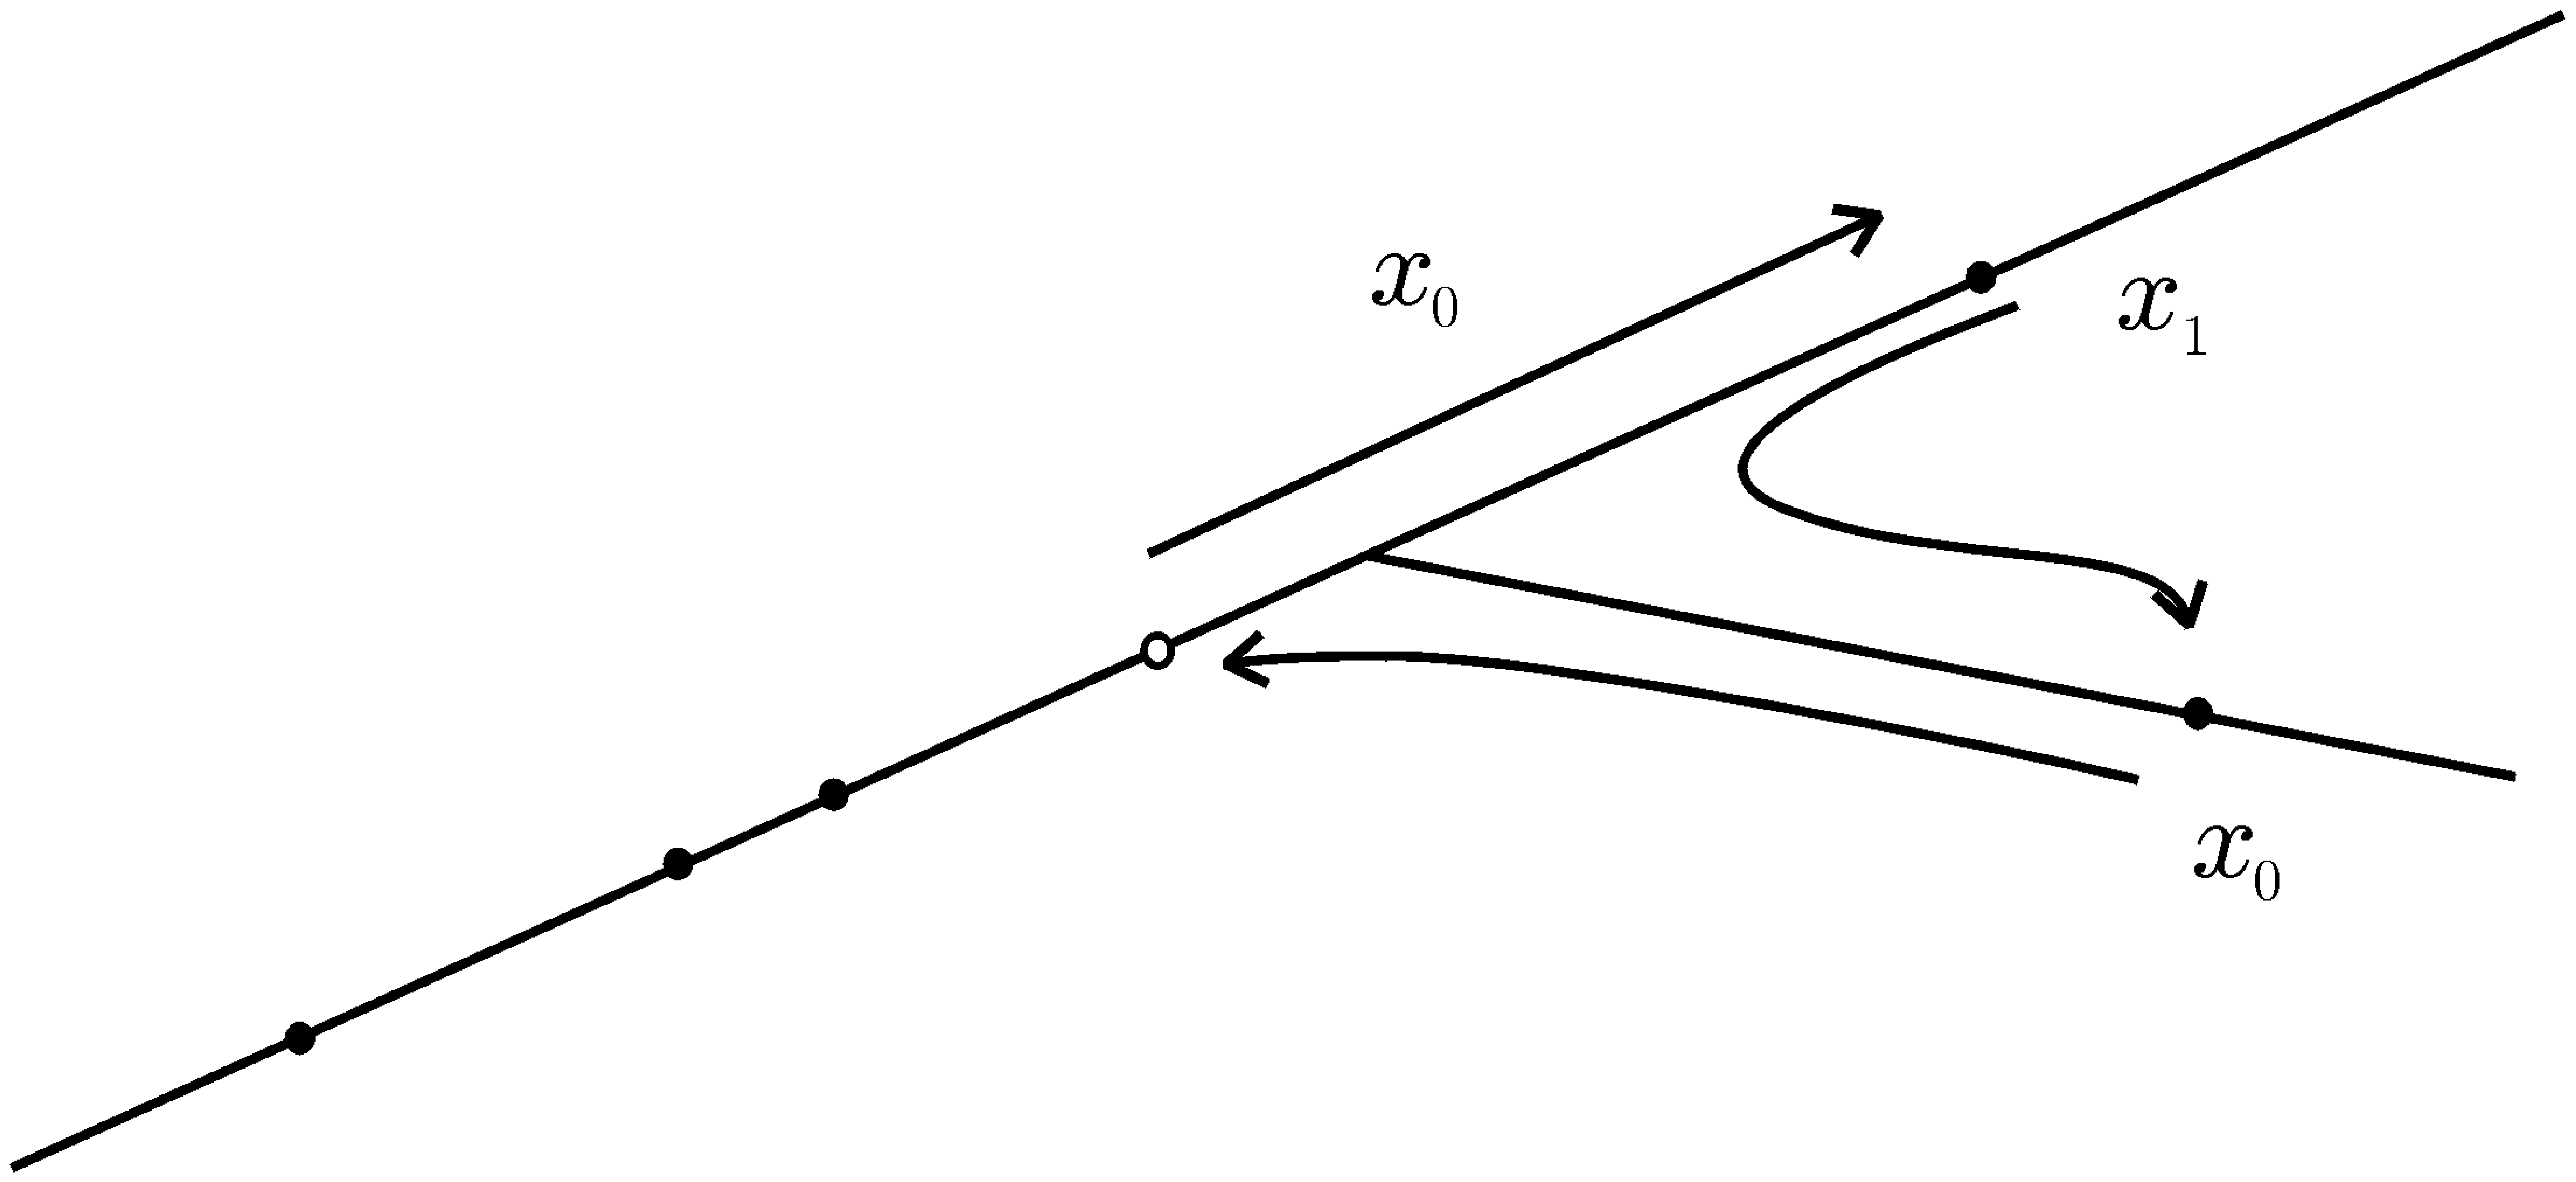
\includegraphics[width=0.5\textwidth]{pict/pict01-6.eps}
\end{center}
 \bigskip
 \refstepcounter{ris}\label{r1-6}

 \centerline{Рис.~\theris}
 \bigskip
\end{figure}


%%%%%%%%%%%%%%%%%%%%%%%%%%%%%%%%%%%%%%%%%%%%%%%%%%%%%%%%%%
%\noindent \hskip3.0cm {рис. 6}
%\bigskip

\noindent
Так что классическая задача интерполяции ограничена
рассмотрением ее на отрезке.

\begin{task}
При чем здесь отрезок? Пусть {$f_k(x) \in \bR^m$}\  $\forall\ x \in K \subset
\bR^M$\ {$(k=0,1,\ldots,n).$} На каких множествах $K$ существуют
непрерывные интерполяционные системы, а для каких не существуют?
\end{task}

При $m \ge 2$ окончательного ответа на эти вопросы нет. Известно (теорема
Мерхьюбера), что при $m=1$ и $n \ge 1$ компактное множество $K$ должно быть гомеоморфно
части
{окружности или всей окружности.
В последнем случае $n$ должно быть четным, т.\,е.} {число базисных функций -- нечетным.
}

 % Лекции Сергея Борисовича Стечкина
% Внесены исправления Ю.Н.Субботина и Н.И.Черныха, версия 30.06.2009
% Внесены исправления Н.И.Черныха, версия 29.07.2009
% Внесена грамматическая и ТеХ-правка М.Дейкаловой, версия 05.08.09

\chapter{Оценка остаточного члена интерполяции.\\
Многочлены Чебышева} %%{Лекция 2.}

\section{Оценка остаточного члена}

Пусть {$\{x_k\}^n_{k=0}$}~-- узлы интерполяции на $[a,b]$ и функция $f$ имеет непрерывную
${n+1}$ производную на $[a,b],$\ {$p_n(x,f)$~--
соответствующий} интерполяционный многочлен {Лагранжа} для $f,$\ $R_n(x,f)=f(x)-p_n(x,f)$~--
остаточный член интерполяции. Мы получили оценку
для $\|f(\cdot)-p_n(\cdot ,f)\|_C$ через наилучшее приближение
$E_n(f, \Cal P_n)_C$ (см. неравенство Лебега) и, значит, {(}так как $E_n(f,
\Cal P_n)_C \le \|f\|_C${)} через $\|f\|_C.$ Получили также оценку
$\|R_n(\cdot ,f) \|_C$ через максимум $f^{(n+1)}$ на отрезке, т.\,е. через
$\|f^{(n+1)}\|_C$ (см. {следствие из теоремы~\ref{t1-1})}. Следовательно, имеем оценки
\[
  \|f(\cdot )-p_n(\cdot ,f)\|_C \le
               \begin{cases}
                   \Cal K_0 \|f\|_C ,\\
                   \Cal K_{n+1} \|f^{(n+1)}\|_C ,
               \end{cases}
\]
где $\Cal K_0$ и $\Cal K_{n+1}$ -- соответствующие
независящие от функции константы. Попробуем оценить $\|R_n(\cdot ,f)\|_C$ через
{$\|f^{(m+1)}\|_C,$} т.\,е. получить оценки
\begin{equation}\label{lab1}
  \|R_n(\cdot ,f) \|_C \le  \Cal K_{m+1} \|f^{{(m+1)}}\|_C
\end{equation}
и для других $m,$ где $K_{m+1}=K_{m+1}(n)$ не зависят от $f.$
Если такие оценки справедливы, то, взяв функцию $f\in {\cal P}_m$,
у которой {$\|f^{(m+1)}(\cdot )\|_C=0$} получим, что $\|R_n(\cdot ,f)
\|_C=0,$ т.\,е. $f(x) \equiv p_n(x ,f)$ {~--} многочлен степени не выше
$n.$ Так что получаем {необходимое} ограничение на {числа $m,$}
для которых могут быть верны эти оценки: {$m \le n.$} Оценить $\|R_n(\cdot ,f) \|_C$
через нормы производных более высокого порядка нельзя,
так как из условия $f^{(m+1)}(x) \equiv 0,$~ $m > n,$ не следует, вообще
говоря, что $f(x) \equiv p_n(x ,f)$ (например, если $f$ есть
многочлен порядка {$m>n$}).

\begin{lemma}
Условие $m \le n$ является и достаточным условием для справедливости
оценки~$(\ref{lab1}).$
%$\|R_n(\cdot ,f) \|_C$
%через {$\|f^{(m+1)}(\cdot )\|_C.$}
\end{lemma}

\begin{proof}
Интерполяционная формула Лагранжа для $f$ имеет вид
\[
  p_n(x,f)=\sum\limits_{k=0}^n f(x_k) l_k(x).
\]
Используя тождество Коши $\sum\limits_{k=0}^n l_k(x) \equiv 1,$ получаем
$$
R_n(x,f)=f(x)-\sum\limits_{k=0}^nf(x_k)l_k(x)=\sum\limits_{k=0}^n \{f(x)-f(x_k) \} l_k(x).
$$
Запишем для $f(y)$ формулу Тейлора порядка $m$ в точке $x$ с остаточным
членом в интегральной форме
\[
  f(y)=f(x)+p(x,y)+\frac{1}{m!}\int_x^y (y-t)^m f^{(m+1)}(t)dt,
\]
где $f(x)+p(x,y)=q_x(y)$~-- многочлен Тейлора функции $f$ в точке $x.$ В частности,
\[
 f(x_k)=f(x)+q_x(x_k)+\frac{1}{m!}\int_x^{x_k} (x_k-t)^m f^{(m+1)}(t)dt,
\]
где
$$
q_x(x_k) = \sum\limits_{s=1}^m\frac{1}{s!}f^{(s)}(x)(x_k-x)^s
$$
($q_x(x_k)$~-- не многочлен по $x$).

Подставим $f(x_k)$ в выражение для $R_n(x,f),$ при этом учтем, что в
силу третьего тождества Коши \eqref{f1-1} при $m \le n$
$$
\sum\limits_{k=0}^n q_x(x_k)l_k(x)=\sum\limits_{{s=1}}^m{\frac{1}{s!}f^{(s)}(x)
 \sum\limits_{k=0}^n{(x_k-x)^s}l_k(x)}\equiv
0.
$$
{Получим}
\[
{  R_n(x,f)=-\frac{1}{m!} \sum\limits_{k=0}^n l_k(x)
                         \int_x^{x_k} (x_k-t)^m f^{(m+1)}(t)dt=
                         \int_a^b K_{n,m}(x,t,\{x_k\}) f^{(m+1)}(t)dt,}
\]
{Можно проверить, что ядро $K_{n,m}(x,t,\{x_k\})$} этого
выражения при каждом $x$ только при $m=n$ не {меняет знак при $t \in
[a,b]$} и только в этом случае можем,
{применив теорему о среднем,} записать
\[
  R_n(x,f)=f^{(n+1)}(\xi) \cdot A(x)\qquad {(\xi = \xi(x, f, K_{n,n})),}
\]
где $A(x)$ от $f$ не зависит. {Но во} всех {рассматриваемых} случаях {(т.\,е.
при $m \le n$)} получим оценку
\[
  |R_n(x,f)| \le \|f^{(m+1)}(\cdot )\|_C
        \int_a^b |K_{n,m}(x,t,\{x_k\})| dt,\qquad x \in [a,b],
\]
из которой следует требуемое неравенство~(\ref{lab1}).
\end{proof}

\section{Многочлены Чебышева}

Многочленами Чебышева $T_n(x)$ {называются функции}
$$
  T_n(x)=\cos (n\arccos x) \qquad (n=0,1,\dots ),\qquad  x \in [-1,1].
$$
Это, действительно, многочлены: положим $x= \cos \theta$,~ {$\theta \in [0, \pi],$} тогда
%\begin{multline*}
$$
\begin{aligned}
T_n(x) &=\cos (n \arccos x)= \cos n\theta = {\frac{1}{2}(e^{in\theta} +
e^{-in\theta})
=} \\
   &=\frac{1}{2}\{(\cos \theta +i \sin \theta)^n+(\cos \theta -i \sin \theta)^n\}.
\end{aligned}
$$
%\end{multline*}
{Следовательно, при $|x| \le 1$}
$$
T_n(x)=\frac{1}{2}\{(x +i \sqrt{1-x^2})^n+(x -i \sqrt{1-x^2})^n\}.
$$
Из последнего выражения видно, что мнимые части {здесь} уничтожаются, {а в}
{вещественной части радикалы отсутствуют}.

\begin{ex}
{Как многочлен, функция $T_n(x)$ определена при всех $x$. Найти} {для него
представление при $|x| > 1$, аналогичное последней формуле.}
\end{ex}

\section{Основные свойства многочленов Чебышева \\
(выражаемые равенствами)}

\vspace{-2mm}
{\bf 1. Рекуррентная формула}
\vspace{3mm}

При $n=0$ и $n=1$ имеем $T_0(x) \equiv 1,$ $T_1(x) \equiv x.$ Из тригонометрического тождества
\[
  \cos (n+1)\theta =2 \cos \theta \cos n \theta -\cos (n-1)\theta
  \qquad (x = \cos{\theta})
\]
следует {рекуррентная формула}
\[
  T_{n+1}(x)=2x T_n(x)-T_{n-1}(x) \qquad (n=1,2,\dots ).
\]
{Имеем также}
$$
 {T_n'(x)=n \sin ({n} \arccos{x})\cdot \frac{1}{\sqrt{1-x^2}} = \frac{n\sin
 n\theta}{\sin{\theta}}.}
$$

Из рекуррентной формулы следует, что коэффициент при старшей степени многочлена
{$T_n(x)$ при $n \ge 1$} равен $2^{n-1}$, так что
\[
  T_n(x)=\cos (n \arccos x) =2^{n-1} x^n+\cdots .
\]
Все нули этого многочлена $x_k=\cos \dfrac{2k-1}{2n}\pi$
$(k=1,2,\dots ,n)$ лежат в~$(-1,1).$ {Точками} экстремумов
на $[-1,1]$ являются {точки} $\widetilde x_k=\cos \dfrac{k
\pi}{n}$ {$(k=0,1,\dots ,n),$} $T_n(\widetilde x_k)=(-1)^k,$
причем при {$k\ne 0$} и {$k \ne n$} выполнено {условие
$T_n'(\widetilde x_k) = 0,$ а $T_n'(1)=n^2,$}\
{$T_n'(-1)=(-1)^{n-1}n^2$. С ростом $n$ нули и точки
экстремума уплотняются у концов} {отрезка $[-1,1]$} (сравним
рис.~\ref{r2-1} и \ref{r2-2}).

%%%%%%%%%%%%%%%%%%%%%%%%%%%%%%%%%%%%%%%%%%%%%%%%%%%%%%
%\hbox to 0.5cm {}{\special{em:graph pict7.pcx}}
%\vspace{6cm} \vspace{5mm} \noindent
%\begin{picture}(0,170)
% \put(0,160){\special{em: graph pict2-1.pcx}}
% \end{picture}

\begin{center}
\begin{picture}(290,100)
\includegraphics[width=0.95\textwidth]{pict/pict02-1.eps}
\end{picture}
%\bigskip
\centerline{\normalsize Рис.~\theris}

\refstepcounter{ris}\label{r2-1}
\end{center}


%\vspace{-3mm}
{\bf 2. Производящая функция}
\vspace{3mm}

Если дана последовательность $\{A_n\},$ то {ее} производящей функцией называется
такая функция $F,$ коэффициенты Тейлора которой равны $A_n.$

Вычислим {$\sum\limits_{n = 0}^{\infty} \cos (n\theta )\ {t^n}.$}
Это действительная часть степенного ряда
\[
  \sum\limits_{{n=0}}^{\infty}\, \exp{(i n\theta)}\ t^n=\frac{1}{1-t\exp{(i \theta)}}
 { =\frac{1-t\exp(-i\theta)}{1-2{t}\cos{\theta}+t^2},}
\]
так что
\[
  \sum\limits_{{n=0}}^{\infty}\, \cos (n\theta )\ {t^n}=
                      \frac{1-t \cos \theta}{1-2t\cos \theta +t^2}
\]
и если $x=\cos \theta,$ то получаем производящую функцию {$F(t)$} для {последовательности}
многочленов Чебышева:
\[
  \sum\limits_{n=0}^{\infty} T_n(x)\,t^n=\frac{1-tx}{1-2tx+t^2}.
\]
{Заменим здесь $x$ на $-x$. Получим}
$$
{\sum\limits_{n=0}^\infty{T_n(-x)t^n} = \sum\limits_{n=0}^\infty{T_n(x)(-t)^n}}
$$
{и, следовательно, $T_n(-x)=(-1)^nT_n(x)$. Конечно, это
свойство можно вывести и из} {явного представления для
$T_n$.}

\ex Как растут {$|T_n(x)|$} в точках $|x|>1$ {с ростом $n$?}

\noindent {У к а з а н и е.\ \ Воспользоваться представлением}
$$
{T_n(x)=\frac{1}{2}\left \{(x +\sqrt{x^2-1})^n+(x -
\sqrt{x^2-1})^n \right\}, \qquad |x|>1.}
$$

\vspace{3mm}
{\bf 3. Дифференциальное уравнение}
\vspace{3mm}

Дифференциальное уравнение, которому удовлетворяют $T_n$:
\[
  (1-x^2)y''-xy'+n^2y=0\qquad (n=0,1,\dots ).
\]
\ex Проверить.

Будем искать {коэффициенты многочлена}
$$
{ T_n(x)=\sum\limits_{k=0}^n a_kx^{n-k}}
$$
{при $n\ge 2$, зная, что он} удовлетворяет этому уравнению. {Знаем также, что}
$a_0=2^{n-1}$ {и} $a_1=a_3=\cdots =0,$ {так как $T_n(-x)=(-1)^nT_n(x).$} Тогда,
подставив в дифференциальное уравнение, получим рекуррентное соотношение
\[
  a_{2k}=-\frac{(n-2k+2)(n-2k+1)}{4k(n-k)}a_{2k-2}.
\]
Следовательно,
\[
  a_{2k}=\frac{(-1)^k n(n-1)\cdots (n-2k+1)}{4^kk!(n-1)\cdots (n-k)}\,{a_0}=
  (-1^k)
  \frac{n}{n-k}C^k_{n-k}2^{n-2k-1}
\]
{и}
$$
  T_n(x)=\sum\limits_{k=0}^{[n/2]} a_{2k}x^{n-2k}.
$$

\begin{Remark}
Несмотря на то, что многочлены Чебышева ограничены единицей на $[-1,1],$ его
коэффициенты при больших $n$ очень большие.
\end{Remark}

\vspace{3mm}
{\bf 4. Ортогональность}
\vspace{3mm}

{Справедливы равенства}
\[
{\frac{2}{\pi}} \int_{-1}^1 \frac{T_n(x)T_m(x)}{\sqrt{1-x^2}}dx={\delta_{n,m}}.
\]

\begin{ex}
{Проверить, сделав замену $x=\cos{\theta}$~ $(0 \le \theta \le \pi)$.}
\end{ex}

\section{Экстремальные свойства многочленов Чебышева}

%\vspace{3mm}
{\bf 1. Первое экстремальное свойство}
\vspace{3mm}

Нормированный многочлен Чебышева $\widetilde T_n(x)=\dfrac{T_n(x)}{2^{n-1}}$ есть многочлен, наименее уклоняющийся от нуля на $[-1,1]$ среди
всех многочленов со старшим коэффициентом $1,$ т.\,е. имеет место {следующее утверждение.}

\begin{teo} \label{teo1extsvo}
Справедливы равенства
%{\it
%\begin{multline*}
$$
\inf_{p \in \Cal P_n,\ p =x^n+\dots} \|p(\cdot )\|_{C[-1,1]} =
            \|\widetilde T_n(\cdot )\|_{C[-1,1]}=\frac{1}{2^{n-1}}=
$$
$$
=\inf_{p \in \Cal P_{n-1}} \|x^n-p(x)\|_{C[-1,1]}= E_{n-1}(x^n)_{C[-1,1]},
$$
%\end{multline*}
где $$\widetilde T(x)=\dfrac{1}{2^{n-1}}T_n(x)=x^n+\dots$$ -- нормированный
многочлен Чебышева. Наилучшее приближение
$E_{n-1}(x^n)_{C[-1,1]}$ достигается на
многочлене $p(x)=x^n-\dfrac{1}{2^{n-1}}T_n(x)\in {\cal P}_n$ {и только на нем}.
\end{teo}

\begin{proof}
Основная идея доказательства заключается в подсчете числа нулей. Пусть есть многочлен
$p \in \Cal P_n$ %с той же нормировкой,
{со старшим коэффициентом, равным $1$,}
но {такой, что}
$$
  \|p(\cdot )\|_{C[-1,1]}  \le \|\widetilde T_n(\cdot )\|_{C[-1,1]}.
$$
Тогда на каждом отрезке, где {$T_n(x)$} изменяется от {$\pm 1$} до {$\mp 1,$ т.\,е. на }
{отрезках $[\widetilde x_k, \widetilde
x_{k+1}]\ (\widetilde x_k=\cos \dfrac{k\pi}{n}$, \
$k={0,1,}\ldots,n$)} разность {$r_{n-1}(x)=\widetilde T_n(x)-p(x)$} обращается в нуль
{(при этом мы учитываем, что если $r_{n-1}=0$ в общем конце двух} {таких отрезков,
то там $T'$ и $p'$ обращаются в нуль и, значит, это
двойной нуль} {разности $r_{n-1}(x)$, см.~рис.~\ref{r2-2}).} {Таким образом,}
степень многочлена $r_{n-1}$ не выше $n-1,$ {а число его
нулей с учетом кратности $\ge n.$} {Следовательно,} $r_{n-1} \equiv 0,$ {$p(x)
\equiv \widetilde T_n(x),$ откуда вытекают все утверждения
теоремы~\ref{teo1extsvo}.} %\pagebreak

%%%%%%%%%%%%%%%%%%%%%%%%%%%%%%%%%%%%%%%%%%%%%%%%%%%%%% %\hbox to 0.5cm {}{\special{em:graph pict8.pcx}} %\vspace{6cm} \vspace{5mm} \noindent
%\begin{picture}(0,210)
% \put(0,190){\special{em: graph pict2-2.pcx}}
% \end{picture}
% \refstepcounter{ris}\label{r2-2}
\begin{center}
\begin{picture}(320,130)
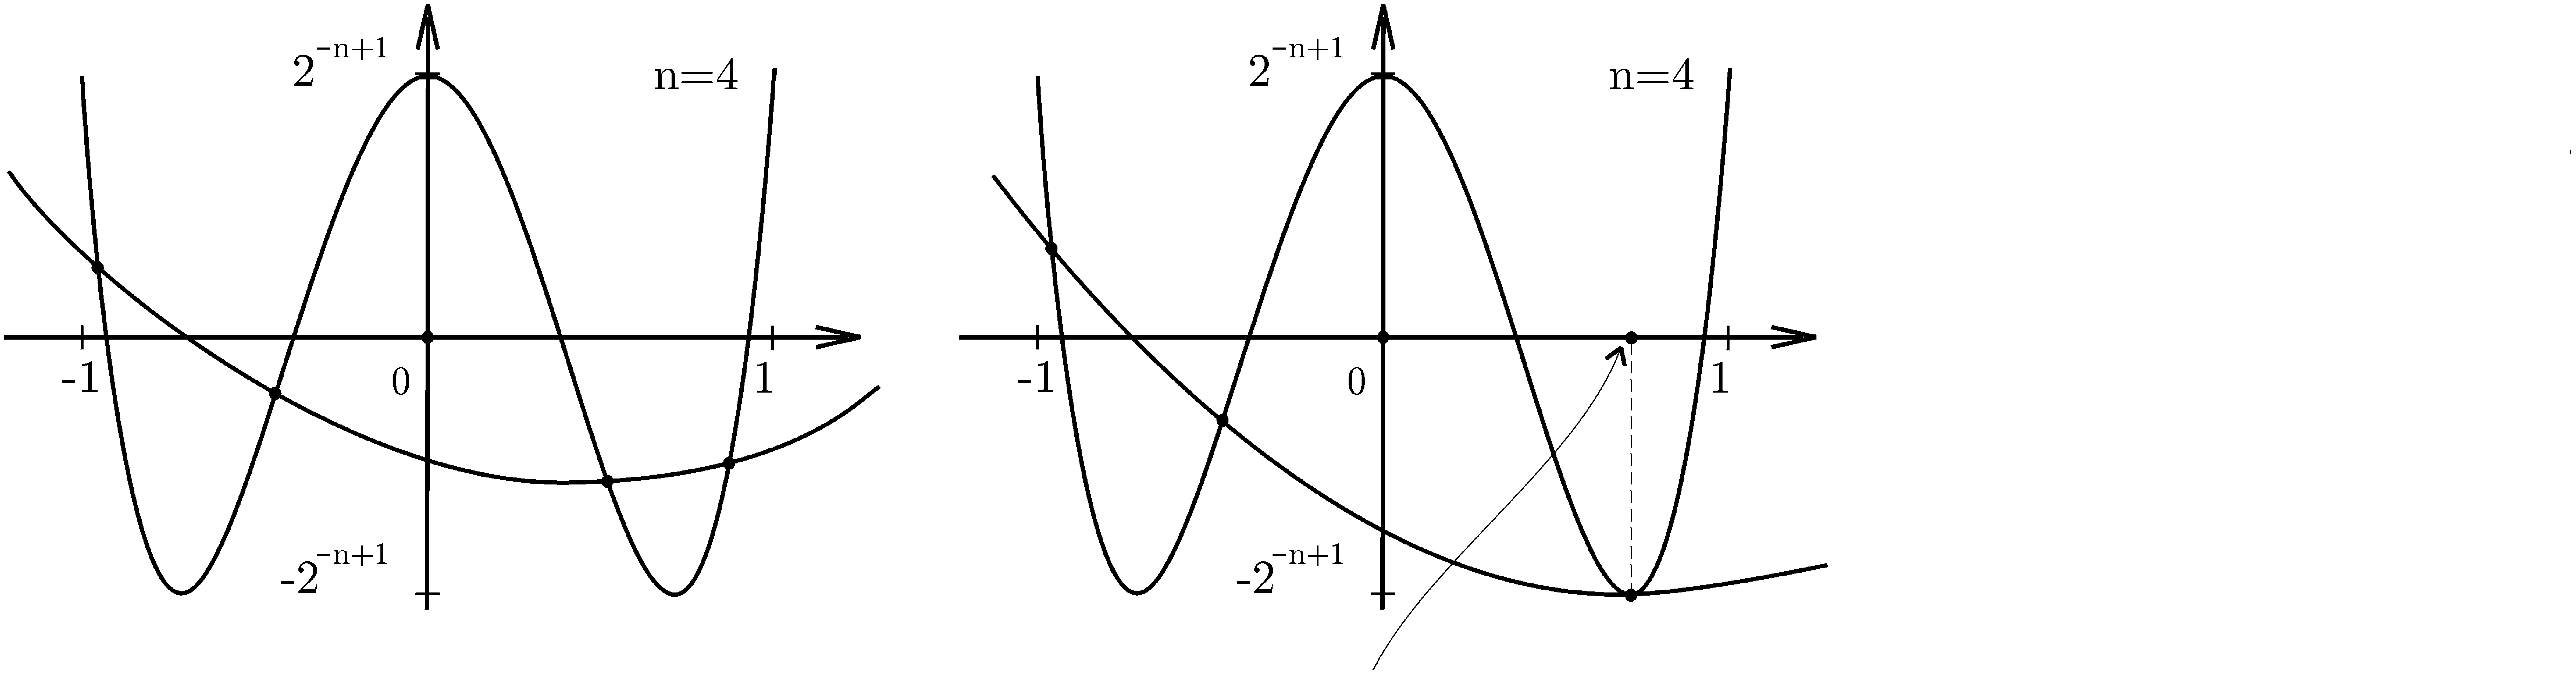
\includegraphics[width=0.99\textwidth]{pict/pict02-2.eps}
\end{picture}
%\bigskip

\refstepcounter{ris}\label{r2-2}
\end{center}

%\centerline{Рис.~\theris}
 \hspace{9.5cm} {Двойной нуль}


 \centerline{\normalsize Рис.~\theris}
\end{proof}

\vspace{2mm}
{\bf 2. Второе экстремальное свойство}
\vspace{3mm}

\begin{lemma}
Пусть {$p \in \Cal P_n,$~ $|p(x)| \not\equiv |T_n(x)|\cdot \|p\|_{C[-1,1]},$} и пусть
$\xi \in \bR,$~ $|\xi |>1.$ Тогда
\[
{ |p(\xi )| < |T_n(\xi)|\cdot \|p(\cdot )\|_{C[-1,1]}.}
\]
{Равенство хотя бы в одной точке $\xi$ вне $[-1,1]$ здесь возможно, только если}
{$p(x)\equiv 0$ {или
$\dfrac{|p(x)|}{\|p\|_{C[-1,1]}}\equiv |T_n(x)|.$}}
\end{lemma}

Д о к а з а т е л ь с т в о\ \ от противного. {Предположим,} {что $\exists\ \xi
\not \in [-1,1]$ :} {$|p(\xi)|
\ge |T_n(\xi)|\cdot\|p\|_{C}$.} Разность
{$q(x)=\dfrac{p(x)}{\|p_n\|_{C[-1,1]}}-T_n(x)$} {-- нетривиальный} многочлен степени
{не выше} $n$ и не может иметь {больше $n$
нулей.} { Пусть для определенности $\xi<-1$,~ $\dfrac{p(\xi)}{\|p\|_{C}}
\ge T_n(\xi) > 0$ (т.\,е. $n$ -- четное, $p(\xi)>0$).}
{Считаем нули. Ясно, что на отрезке $[\xi,-1]$ найдется точка}
{$\xi_0,$ в которой $q(\xi_0)=0.$}

%%%%%%%%%%%%%%%%%%%%%%%%%%%%%%%%%%%%%%%%%%%%%%%%%%%%%%
%\hbox to 0.5cm {}{\special{em:graph pict9.pcx}} %\vspace{6cm} \vspace{5mm}
 %\bigskip
 %\begin{picture}(110,200)
 %\put(110,200){\special{em: graph pict2-3.pcx}}
 %\end{picture}
 %\refstepcounter{ris}\label{r2-3}

 %\centerline{Рис.~\theris}
 %\bigskip

 \begin{center}
\begin{picture}(160,128)
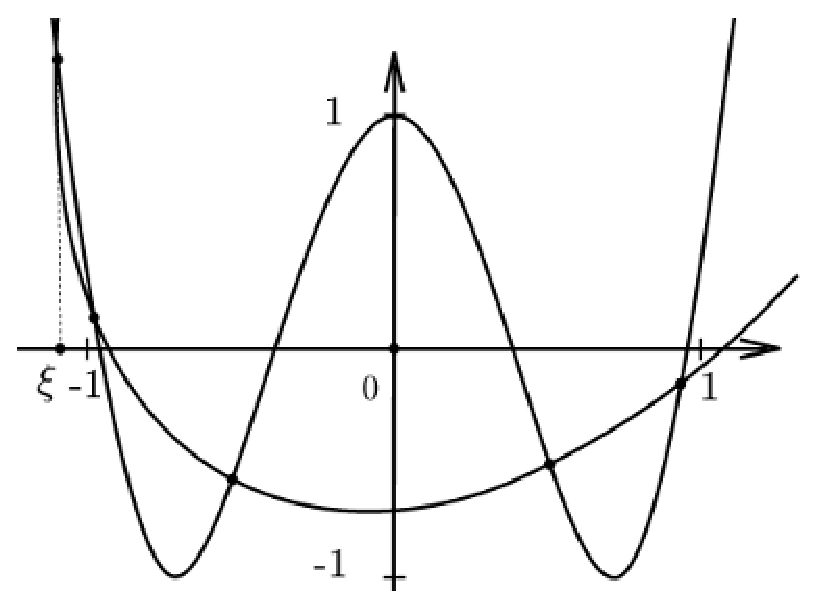
\includegraphics[width=0.34\textwidth]{pict/pict02-3.eps}
\end{picture}
\vspace{5mm}
\refstepcounter{ris}\label{r2-3}
\end{center}

\centerline{\normalsize Рис.~\theris}


%%%%%%%%%%%%%%%%%%%%%%%%%%%%%%%%%%%%%%%%%%%%%%%%%%%%%%%%%% %\noindent \hskip3.0cm {рис. 9}

%\centerline{рис.9}


\noindent

{Далее, график полинома $y{(x)}=\dfrac{p(x)}{\|p\|_{C}}$ на отрезке
$[-1,1]$ не выходит за полосу $|y| \le 1.$ Поэтому, рассуждая как при
доказательстве теоремы~\ref{teo1extsvo}, получаем, что $q(x)$ имеет на
$[-1,1]\quad n$ нулей с учетом их кратности. Если к тому же $\xi_0 < -1$
{(см. рис.~\ref{r2-3})}, то получаем $q(x) \equiv 0$ на $\bR.$
Если же $\xi_0=-1$ и $q(x) \ne 0$ на промежутке $[\xi, -1),$ то рассуждать
нужно чуть потоньше. Во-первых, может оказаться, что $\xi_0=-1$~-- нуль
второго порядка~-- двойной корень $q.$ Ясно, что один из них не вошел в
число учтенных $n$ нулей на отрезке $[-1,1],$ так как из двойных нулей
были учтены только совпадающие с некоторыми из $\widetilde x_k=\cos
\dfrac{k\pi}{n}$~ $(k=1,2,\ldots,n-1).$}

{Вторая возможность~-- $q'(\xi_0) \ne 0$ {$(\xi_0=-1)$.}
Тогда $q(x)$ в
точке $\xi_0=-1$ меняет знак с $+$ на $-$, график $p(x)$ в
правой полуокрестности точки {$\xi_0$} окажется ниже
графика~$T_n.$ Следовательно в обоих случаях {на промежутке $[-1,\widetilde{x}_{n-1}]$}
{у полинома $q(x)$ будет не менее двух нулей,} общее число
нулей будет $\ge n+1.$ Значит, опять $q(x) \equiv 0$ на $\bR,$
что противоречит предположению.}

{Общий случай (без предположений $\xi < -1$ и $n$~-- четное) сводится к
рассматриваемому заменой $p$ и $T_n$ на $-p,\ -T_n$ и/или $T_n(x)$ на $T_n(-x)$. Лемма
доказана.}

%\end{proof}


{Таким образом, если $\|p_n\|_{C[-1,1]} \le 1,$~ $p_n \in \Cal P_n,$ и
$|\xi|>1,$ то $|p_n(\xi)| \le |T_n(\xi)|.$}

\ex {Доказать, что если $p \in \Cal P_n$ и}
$\|p(\cdot )\|_{C[-1,1]} \le 1,$ то $|p'(1)| \le T_n'(1)$ (для доказательства
опять считаем нули), {см. рис.~\ref{r2-4}}.

{Имея ввиду это свойство, $T_n$} называют многочленом сравнения.

%%%%%%%%%%%%%%%%%%%%%%%%%%%%%%%%%%%%%%%%%%%%%%%%%%%%%% %\hbox to 0.5cm {}{\special{em:graph pict10.pcx}} %\vspace{6cm} \vspace{5mm}
%\begin{picture}(100,170)
% \put(100,160){\special{em: graph pict2-4.pcx}}
% \end{picture}
% \refstepcounter{ris}\label{r2-4}

% \centerline{Рис.~\theris }
% \bigskip


 \bigskip
\begin{figure}[ht]
\begin{center}
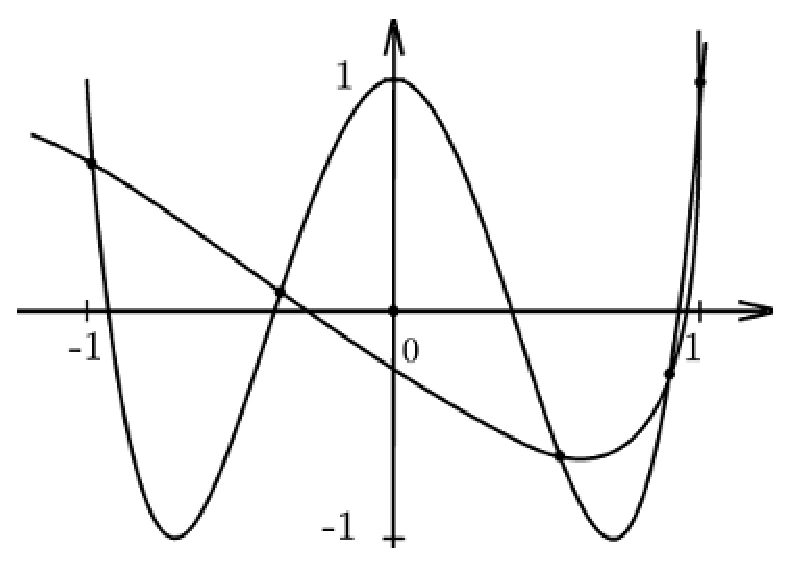
\includegraphics[width=0.35\textwidth]{pict/pict02-4.eps}
\end{center}
 \bigskip
 \refstepcounter{ris}\label{r2-4}

 \centerline{Рис.~\theris}
 \bigskip
\end{figure}




\begin{Remark}
Из леммы~2.2 следует, что если $[-a,a] \supset [-1,1]$
 и $p_n \in \Cal P_n,$ то справедливо неравенство
\[
  \|p(\cdot )\|_{C[-a,a]} \le \|T_n(\cdot )\|_{C[-a,a]}\cdot \|p(\cdot )\|_{C[-1,1]},
\]
{где знак равенства возможен только при $p(x)\equiv 0$ или $p(x)\equiv\pm T_n(x)
\|p(\cdot )\|_{C[-1,1]}$.}
\end{Remark}

 % Лекции Сергея Борисовича Стечкина
% Внесены исправления Ю.Н.Субботина и Н.И.Черныха, версия 30.06.2009
% Внесены исправления Н.И.Черныха, версия 29.07.2009
% Внесена грамматическая и ТеХ-правка М.Дейкаловой, версия 05.08.09

\chapter{Многочлены Чебышева (продолжение).\\ {Интерполяция (приложения)}}  %%{Лекция 3.}

{\section{Теорема В.\,А.\,Маркова }}

{\bf 1. Третье экстремальное свойство многочленов Чебышева}

\ \

Рассмотрим задачу В.\,А.\,Маркова. При фиксированных {$m\in \bN$ и $n \ge m$}
среди всех многочленов степени
{$n$ с коэффициентом} $a_m=1,$ какой многочлен наименее
уклоняется от нуля {на $[-1,1]$}?


Для ее решения предварительно докажем следующую лемму.

\begin{lemma}[Лемма о нулях]\label{l2-3}
Пусть дан {отличный от тождественного нуля} $(N+1)$-членный полином
$\sum\limits_{k=0}^{N}A_kx^{\lambda_k},$ $0 \le \lambda_0 < \lambda_1 < \cdots <
\lambda_N.$ Тогда на $(0,\infty )$ он может иметь не более $N$ нулей.
\end{lemma}

 %\begin{proof}
Д\;о\;к\;а\;з\;а\;т\;е\;л\;ь\;с\;т\;в\;о\ \ индукцией по $N.$
При $N=0$ {и $A_0 \ne 0$} {полином} $A_0 x^{\lambda_0}$
не имеет нулей на $(0, \infty ).$ При $N=1$ {и $|A_0|+|A_1|
\ne 0$ полином} $A_0 x^{\lambda_0}+A_1
x^{\lambda_1}=x^{\lambda_0}
                                   (A_0+A_1 x^{\lambda_1-\lambda_0})$
может иметь не более одного нуля на~$(0,\infty).$ Пусть
{любой $(N+1)$-членный полином
$\sum\limits_{k=0}^{N}A_kx^{\lambda_k} \not \equiv 0$ } имеет
не более $N$ нулей на~$(0, \infty).$ Тогда
{$G(x)=\sum\limits_{k=0}^{N+1}A_kx^{\lambda_k}=
                        x^{\lambda_0}\sum\limits_{k=0}^{N+1}A_kx^{\lambda_k-\lambda_0}=
                        x^{\lambda_0}\cdot F(x)$}
имеет столько нулей на $(0, \infty ),$ сколько их имеет
$F(x)=\sum\limits_{k=0}^{N+1}A_kx^{\lambda_k-\lambda_0},$
при этом можно считать, что $A_{N+1} \ne 0$ {(иначе
$G(x)$~-- $(N+1)$-членный полином).} Но {тогда}
$F'(x)=\sum\limits_{k=1}^{N+1}B_kx^{\lambda_k-\lambda_0-1}$~-- {$(N+1)$}-членный
{не тривиальный} полином
{$(B_{N+1}=(\lambda_{N+1}-\lambda_0) A_{N+1}\ne 0)$}, который по
предположению индукции имеет не более $N$ нулей. Следовательно,
{по теореме Ролля} $F(x)$ имеет не более $N+1$ нулей. Лемма
доказана. %\end{proof}

Теперь вернемся к задаче В.\,А.\,Маркова.

Пусть $C=C[-1,1],$~ $p_n \in {\Cal P}_n,$~ $p_n(x)=\sum\limits_{k=0}^{n}a_kx^k,$~
${\Cal Q}^m_{n}=\{p_n(x):\ p_n\in {\Cal P}_n,\ a_{m}=1\}.$

%\begin{task}
Требуется найти $p_n^* \in \Cal P_n$
такой, что
\[
  \inf_{p_n \in {\Cal Q}^m_n} \|p_n(\cdot)\|_{C[-1,1]} =
  \min_{p_n \in {\Cal Q}^m_n} \|p_n(\cdot)\|_{C[-1,1]} =
  \|p^*_n(\cdot)\|_{C[-1,1]}.
\]
Эту задачу можно также рассматривать как задачу о
наилучшем приближении, именно
\[
  \inf_{p_n \in {\Cal Q}^m_n} \|p_n(\cdot)\|_{C[-1,1]} =
  \inf_{q \in {\Cal P}_n,\ a_m=0} \|x^m-q(x)\|_{C[-1,1]} =
  E(x^m,L_n^m)_{C[-1,1]},
\]
где $L_n^m=\{p\in {\Cal P}_n:\ a_m=0\}$ -- конечномерное линейное подпространство пространства
$C,$ которое обладает как и ${\Cal P}_n$ свойством: если возьмем
четную или нечетную часть какого-нибудь многочлена из этого
подпространства, то снова получим многочлен из этого подпространства.
%\end{task}

Заметим, что среди многочленов {с $a_m=0$}, которые приближают функцию $x^m$
наилучшим образом, {найдется наилучший} многочлен {той же
четности, что} $x^m$.

Действительно, пусть $m$ четное и $p_n(x)$~-- наилучший многочлен из нашего
подпространства. Тогда {$q_n(x)=\dfrac{1}{2}\{p_n(-x)+p_n(x)\}$}
тоже многочлен из того же подпространства, но уже четный, и приближает
{функцию $x^m$} не хуже:
\[
  \|x^m-q_n(x)\|_C=\Bigl\|\frac{1}{2}(x^m-p_n(x))+
                     \frac{1}{2}((-x)^m-p_n(-x))\Bigr\|_C \le
  \|x^m-p_n(x)\|_C.
\]
Следовательно, четные функции приближаются четными
многочленами наилучшим образом. Аналогичный вывод можно сделать для нечетных
функций и нечетных многочленов. Отсюда следует, в частности,
что если $m$ и $n$ разной четности, то наилучший многочлен
{$q_n^*$} той же четности, что и $m$, должен иметь степень
$n-1,$ и следовательно, {$q_n^*\equiv q_{n-1}^*.$}

 Введем в рассмотрение {следующее представление многочлена}
Чебышева:
\[
  T_n(x)=\cos{( n \arccos x)} =\sum\limits_{k=0}^n A_k^nx^k.
\]
\begin{teo}[{В.\,А.\,Марков}]
Если $m$ и $n$ имеют одинаковую четность, то среди всех многочленов степени $n$ с
коэффициентом $a_m=1$ {$(0\le m\le n)$} наименее уклоняется от
нуля многочлен $\dfrac{T_n(x)}{A_m^n},$ с уклонением
\[
  \Bigl\|\frac{T_n(\cdot )}{A_m^n}\Bigr\|_{C[-1,1]}=\frac{1}{|A_m^n|}.
\]
Если же $m$ и $n$ имеют разную четность, то среди всех многочленов степени $n$ имеющих
$a_m=1$ {$(0\le m\le n-1),$} наименее уклоняющимся от нуля является многочлен
$\dfrac{T_{n-1}(x)}{A_m^{n-1}},$ с уклонением
\[
  \Bigl\|\frac{T_{n-1}(\cdot )}{A_m^{n-1}}\Bigr\|_{C[-1,1]}
                                             =\frac{1}{|A_m^{n-1}|}.
\]
\end{teo}

\begin{proof}
Для доказательства надо рассмотреть 4 случая для $m$ и $n$ разных четностей. Докажем
{теорему только в одном случае}, когда $m$ и $n$ четные. Итак, надо доказать, что если
$p_n(x)=\sum\limits_{k=0}^n a_kx^k$~-- произвольный многочлен с $a_m=1$ {и четными
$n$ и $m,$} то
\[
  \| p_{n}(\cdot ) \|_{C[-1,1]} \ge \frac{1}{|A_m^{n}|}.
\]


Пусть это утверждение неверно, т.\,е. пусть существует многочлен
{$p_n(x)$} такой, что
\begin{equation}
\label{Macar}
  \| p_{n}(\cdot ) \|_{C[-1,1]} {<} \frac{1}{|A_m^{n}|}.
\end{equation}
{Многочлен} $p_n$ может {не} быть четным, но тогда {$\dfrac{1}{2}(p_n(x)+p_n(-x))
\in \Cal Q^m_n$} тоже удовлетворяет неравенству~(\ref{Macar}) и будет четным.
{Поэтому далее считаем, что в~(\ref{Macar}) $p_n$ --} {четный многочлен, отличный от
$\dfrac{T_n(x)}{A_m^n}$.} Многочлен Чебышева $T_n(x)$ тоже четный. Рассмотрим многочлен
\[
  R_{n}(x)=\frac{T_n(x)}{A_m^{n}}-p_n(x)=
  \sum\limits_{k=0}^{n/2}b_kx^{2k}{\not\equiv 0,}
\]
{где} $b_{m/2}=0.$ Таким образом, у $R_n(x)$ не более, чем $n/2=l$ не равных нулю
коэффициентов. По {лемме~\ref{l2-3}} о нулях $l$-членный полином
{$R_n(x)\not\equiv0$} может иметь на $(0,\infty)$ и, следовательно, на $(0,1)$ -- не
более $l-1$ нулей. У нас же $T_n(x)$ имеет на $[0,1]$ ровно $n/2+1$ точек
{$\widetilde{x}_k=\cos\dfrac{k\pi}{n} \
 \left(k=0,1,\ldots,\dfrac{n}{2} \right)$} максимального уклонения, в которых
$R_n(x)$ {в силу~(\ref{Macar})} имеет тот же знак, что и $\dfrac{T_n(x)}{A_m^{n}}$ и,
значит, между ними есть $n/2=l$ точек, в которых
$R_n(x)=0.$ Все эти $l$ нулей $R_n(x)$ лежат точно в {интервале} $(0,1),$
{что противоречит предыдущему выводу.} Следовательно, вместо~(\ref{Macar})
имеем противоположное неравенство, которое обращается в равенство при
$p_n(x)\equiv\dfrac{T_n(x)}{A_m^{n}}.$ В остальных случаях теорема
доказывается аналогично.
\end{proof}

\begin{Remark}
В общем случае многочлен наименьшего уклонения не
единственный. Например, при $n=2,$ $m=0$ и $0\le c\le 2$
имеем
{$$
\|1-cx^2\|_{C[-1,1]}=1=\left\|\dfrac{T_2(x)}{A_0^2}\right\|_{C[-1,1]}.
$$}
\end{Remark}



\begin{Corollary}[Оценки коэффициентов многочленов]
Пусть $p_n(x)=\sum\limits_{k=0}^n a_kx^k$ и известна норма
$\|p_n(\cdot )\|_{C[-1,1]}.$ Тогда для $m$ и $n$ одинаковой
четности
\[
  |a_m| \le |A_m^n|\cdot  \|p_n(\cdot )\|_{C[-1,1]},
\]
{а} для $m$ и $n$ разной четности
\[
  |a_m| \le |A_m^{n-1}|\cdot  \|p_n(\cdot )\|_{C[-1,1]}.
\]
\end{Corollary}

\begin{proof} Действительно, например, для $m$ и $n$ {одинаковой}
{четности и $a_m\neq 0$} из теоремы следует {оценка}
\[
  \Bigl\| \frac{p_{n}(\cdot )}{a_m} \Bigr\|_{C[-1,1]}
  \ge \frac{1}{|A_m^{n}|},
\]
а, значит, и требуемое неравенство. {При $a_m=0$ это неравенство тривиальное.}
Следовательно, у многочленов Чебышева коэффициенты одинаковой
со степенью многочлена четности самые большие
{среди многочленов $p_n$ той же степени с $\|p_n\|_{C[-1,1]}\le 1.$}

\begin{ex}
Провести доказательство теоремы Маркова для $m$ и $n$
разной четности.
\end{ex}
\end{proof}

\begin{Remark} Так как $a_m={\dfrac{p_n^{(m)}(0)}{p!}}$,
то {неравенства следствия можно переписать} {в виде}
\[
  |p_n^{(m)}(0)| \le m!\cdot |A_m^n|\cdot  \|p_n(\cdot )\|_{C[-1,1]},
\]
\[
{|p_n^{(m)}(0)| \le |T_n^{(m)}(0)|\cdot \|p_n(\cdot )\|_{C[-1,1]}\qquad (0\le m\le n)}
\]
для $m$ и $n$ одинаковой четности и
\[
  |p_n^{(m)}(0)| \le m!\cdot |A_m^{n-1}|\cdot  \|p_n(\cdot )\|_{C[-1,1]},
\]
\[
{|p_n^{(m)}(0)| \le |T_{n-1}^{(m)}(0)|\cdot \|p_n(\cdot )\|_{C[-1,1]} \qquad (0\le m\le n-1)}
\]
для
$m$ и $n$ разной четности.
\end{Remark}
%\end{proof}

\section{Экстремальная интерполяция на классе $W^{n+1}$}

{\bf 1. Четвертое экстремальное свойство}

\ \

Пусть $a \le x_0<x_1<\dots <x_n\le b$~-- узлы интерполяции на
$[a,b],$ $f \in \G M \subset C^{(n+1)}[a,b]$,~ $p_n(x,f)=\sum\limits_{k=0}^n
f(x_k)l_k(x)$~-- интерполяционный многочлен Лагранжа. Тогда, как мы знаем,
\[
  R_n(x,f)=f(x)-p_n(x,f)=\frac{f^{(n+1)}(\xi)}{(n+1)!} \omega (x),
\]
где $\xi \in [a,b]$ и $\omega(x)=(x-x_0)\cdots (x-x_n).$
Итак, задан класс функций $f \in \G M.$
Как подобрать узлы так, чтобы остаток интерполяционной формулы по всему классу был
наименьший?


Для класса $\G M$
рассмотрим величину
\begin{equation}
\label{estim1}
  \sup_{f \in \G M}\| R_{n}(\cdot ,f,\{x_k\}) \|_{C[-1,1]}
                      =F_n(\G M,\{x_k\}),
\end{equation}
{считая $[a,b]=[-1,1]$.} Задача ставится так: как выбрать узлы,
чтобы величина~(\ref{estim1}) была поменьше, т.\,е. надо найти
\[
  \inf_{\{x_k\}}F_n(\G M,\{x_k\})=\Phi_n(\G M).
\]
{Тогда} для любой функции $f \in \G M $ {и экстремальных узлов будем иметь}
$$
{\| R_{n}(\cdot ,f,\{x_k\}) \|_{C[-1,1]} \le \Phi_n(\G M).}
$$

Заметим, что если для заданной функции выбирать узлы так, чтобы величина
$\|f(\cdot )-p_n(\cdot ,f)\|_{C[-1,1]}$ была наименьшей, то это была бы
{\it другая задача}. Мы ее здесь не решаем.

Выберем в качестве $\G M$ класс
\[
 W^{(n+1)}=\{f{\in C^{n+1}[-1,1]}:\ \|f^{(n+1)}\|_{C[-1,1]}{\le 1}\}.
\]
Найдем
\[
  \inf_{\{x_k\}}\sup_{f \in W^{(n+1)}} \| R_{n}(\cdot ,f,\{x_k\}) \|_{C[-1,1]}.
\]
Зафиксируем $x \in [-1,1].$
Из формулы для остаточного члена в форме Коши
\[
   R_n(x,f)=\frac{f^{(n+1)}{(\xi )}}{(n+1)!} \,\,\omega (x)
\]
следует
\[
  \sup_{f \in \,W^{(n+1)}} | R_{n}(x ,f,\{x_k\}) | \le \frac{|\omega(x)|}{(n+1)!}.
\]
Так как существует функция, для которой $f^{(n+1)}(x) \equiv \pm 1,$ например,
если $f$ есть многочлен со старшим коэффициентом $\pm
\dfrac{1}{(n+1)!},$ то эта оценка обращается в равенство для любого $x \in [-1,1]$:
\[
  \sup_{f \in \,W^{(n+1)}} | R_{n}(x ,f,\{x_k\}) | =\frac{|\omega(x)|}{(n+1)!}.
\]
Значит, и
\[
  \sup_{f \in\, W^{(n+1)}} \| R_{n}(\cdot ,f,\{x_k\}) {\|}_{C[-1,1]} \le
                                \frac{\|\omega(\cdot )\|_{C[-1,1]}}{(n+1)!},
\]
причем {знак равенства будет} опять для той же функции.
Следовательно, задача свелась к нахождению
\[
  \inf_{\{x_k\}} \|\omega(\cdot )\|_{C[-1,1]}.
\]
Так как $\omega (x)=\prod\limits_{k=0}^n (x-x_k)=x^{n+1}+\cdots ,$ то
\[
  \inf_{\{x_k\}} \|\omega(\cdot )\|_{C[-1,1]} \ge
  \inf_{x^{n+1}+\cdots } \|p_{n+1}(\cdot )\|_{C[-1,1]}
  =\|\widetilde T_{n+1}(\cdot )\|_{C[-1,1]}=\frac{1}{2^{n}}.
\]
На самом деле здесь {равенство}, так как класс {всех рассматриваемых} $\omega (x)$~--
{это класс} многочленов со старшим коэффициентом,
равным $1$, и с нулями $x_k \in [-1,1]$\ $(k=0,\dots ,n),$ {а}
нормированный многочлен Чебышева {$\widetilde{T}_{n+1}$} лежит в этом
классе. Следовательно,
\[
  \inf_{\{x_k\}}\sup_{f \in W^{(n+1)}} \| R_{n}(\cdot ,f,\{x_k\}) \|_{C[-1,1]}
  =\frac{1}{(n+1)!}\cdot 2^{-n}
\]
и достигается для {узлов} $\{x_k\},$
являющихся нулями $T_{n+1}.$

\begin{task}
Найти
$$
\inf\limits_{\{x_k\}}\sup\limits_{f \in W^{(r)}}
             \| R_{n}(\cdot ,f,\{x_k\}) \|_{C[-1,1]}
$$
для всех $0 \le r \le n+1.$
\end{task}

Для $r=0$ задача {решена асимптотически,} для $r=n+1$ {решение задачи было} {изложено только
что,} для остальных $r$ задача не решена.

\section{Интерполяция в комплексной области}

Рассмотрим комплексную плоскость $\bC,$ область {$D \subset \bC,$} и пусть $w=f(z)$~--
комплекснозначная функция на $D.$ Пусть в области $D$
задана система различных точек $\{z_k\}$ $(k=0,\dots ,n).$

Построим многочлен $p_n(z,f)$
такой, чтобы
\[
  p_n(z_k)=f(z_k).
\]
Интерполяционная формула Лагранжа и здесь сохраняется:
\[
  p_n(z,f)=\sum\limits_{k=0}^n f(z_k)l_k(z),\qquad {l_k(z)=\frac{\omega(z)}{\omega'(z_k)
  (z-z_k)},\qquad
  \omega(z)=\prod_{m=0}^n(z-z_m)}.
\]
Пусть $f$~-- аналитическая (регулярная) функция в области $D,$ т.\,е. у
$f$ существует $f'$ в $D,$ и пусть $D$ односвязна. Найдем выражение для
остаточного члена. Рассмотрим в $D$ контур $C$ такой, что все точки $z_k$
лежат внутри $C.$ Функция $\dfrac{f(z)}{(z-z_0)\cdots (z-z_n)}$ внутри
$C$ имеет в качестве особенностей только точки $z_0,\dots ,z_n$ и имеет там
{устранимые особенности (если $f(z_k)=0$) или} простые полюса,
так как $z_k \ne z_l$ при $k \ne l.$ Тогда {по теореме о вычетах}
$$
  \frac{1}{2\pi i}\int_C\frac{f(t)\,dt}{(t-z_0)\cdots (t-z_n)}
  =
$$
$$
  =\sum\limits_{k=0}^n \frac{f(z_k)}{(z_k-z_0)\cdots
                    (z_k-z_{k-1})(z_k-z_{k+1})\cdots (z_k-z_n)}
 = \sum\limits_{k=0}^n \frac{f(z_k)}{\omega'(z_k)}.
$$
Зафиксируем точку $z$
внутри контура $C.$
Обозначим
\[
  J(z)=\frac{1}{2\pi i}\int_C \frac{f(t)\,dt}{(t-z)\prod_{k=0}^n(t-z_k)}.
\]
Тогда
\[
  J(z)=\frac{f(z)}{\prod_{k=0}^n(z-z_k)}-
  \sum\limits_{k=0}^n \frac{f(z_k)}{(z-z_k)\omega'(z_k)}
\]
или
%\begin{multline*}
\[
  J(z)\cdot \omega(z)=f(z)-\sum\limits_{k=0}^n
            \frac{f(z_k)\omega(z)}{(z-z_k)\omega'(z_k)}={f(z)-p_n(z,f)=}R_n(z,f)
 =\frac{1}{2\pi i}\int_C \frac{\omega(z)f(t)\,dt}{(t-z)\omega(t)}
\]
%\end{multline*}
для любого $z$ внутри $C.$ Представим $f(z)$ в виде интеграла Коши
\[
{f(z)=}\frac{1}{2\pi i}\int_C \frac{\omega(t)f(t)\,dt}{(t-z)\omega(t)}.
\]
Тогда интерполяционный многочлен
\[
  p_n(z,f)=f(z)-R_n(z,f)=
 \frac{1}{2\pi i}\int_C \frac{\{\omega(t)-\omega(z)\}f(t)dt}{(t-z)\omega(t)}.
\]

\section{Простейшие приложения\\ интерполяционной формулы
Лагранжа}\label{3.4}


Пусть {функция $f$} определена на $[a,b].$ В приложениях {часто} встречается
задача о вычислении значений функционалов и операторов на элементах $f$
функциональных пространств. Конечно, в общем случае здесь
можно говорить лишь о приближенных методах.

%\subsubsection{1. Вычисление {значений} функционала $F(f),$
%т.\,е.числа}
\vspace{3mm}
{\bf 1. Вычисление определенного интеграла}
\vspace{3mm}

Далее рассматривается эта задача на примере простого функционала
$\displaystyle\int_a^b f(x)\,dx.$ При этом для простейшего функционала~-- значения функции в
точке -- считается
известным точный или приближенный метод вычисления.

%\subsubsection{2. Вычисление {значений} оператора A(f){,
%т.\,е. функции $A(f)(x).$}}


%\subsection{Вычисление $\displaystyle\boldsymbol{\int_a^b f(x)dx}$}\label{3.2.1}

Пусть $f(x)\in C[a,b],$ $p_n(x,f)$~-- интерполяционный многочлен, $\{x_k\}$~--
узлы интерполяции, $\{f(x_k)\}$~-- значения функции в узлах.

Сводим интегрирование функции к интегрированию ее интерполяционного многочлена Лагранжа.
Для интеграла получится квадратурная формула.

Итак, заменяем вычисление $\ds\int_a^b f(x)\,dx$ вычислением
\begin{equation}\label{3-3.3}
  \int_a^b p_n(x,f)\,dx=\sum\limits_{k=0}^n f(x_k)\int_a^b l_k(x)\,dx=
  \sum\limits_{k=0}^n A_k f(x_k) \approx \int_a^b
  f(x)\,dx,
\end{equation}
где $l_k(x)=l_k(x;\{x_i\}_0^n),\ A_k=A_k(n).$
Эта формула называется квадратурной формулой {Котеса}, $\{x_k\}^n_{k=0}$~-- узлы
квадратурной формулы, $\{A_k^n\}^n_{k=0}$~-- коэффициенты квадратурной формулы или
коэффициенты Котеса.

Особенностью таких формул является то, что они точны для всех полиномов степени не выше $n,$
т.\,е. если $f$ есть многочлен степени не выше $n,$ то такая формула будет
точной, в {ее правой части} будет знак равенства.

Для того чтобы формула~(\ref{3-3.3})
была точна для любого многочлена степени не выше $n,$ она
должна быть точна для функций $x^p$\ $(p=0,1,\dots ,n).$

Значит, коэффициенты Котеса легко считать:
\[
  \sum\limits_{k=0}^n A_k x^p_k=\int_a^b x^p dx\qquad (p=0,1,\dots ,n).
\]
Это система с определителем Вандермонда, и~$A_k$ определяются однозначно.

Аналогичным образом можно использовать интерполяционные
многочлены Лагранжа для приближенного вычисления значений
других линейных функционалов. Оценки погрешности
соответствующих квадратурных формул выражаются через нормы
функционалов и оценки погрешности интерполяционных формул.

\begin{ex}
Выписать такие оценки для квадратурных формул, используя
результаты из предыдущих лекций.
\end{ex}

Можно строить кубатурные формулы, даже если
интерполяционные формулы написать нельзя. Например, для функций нескольких переменных
на кубе, где вообще нет непрерывных интерполяционных
систем, можно построить кубатурные формулы точные на многочленах заданной степени.
\vspace{3mm}

{\bf 2. Вычисление {значений} оператора ${A(f)},$
{т.\,е. функции ${A(f)(x)}$}}
\vspace{3mm}

Аналогичный прием можно использовать для приближенного
вычисления значений линейного оператора, если умеем
вычислять~$A(l_k)(x).$ Для неограниченных операторов это не
сработает. Например, возьмем
довольно простой аддитивный и однородный оператор~-- оператор дифференцирования.
Задача вычисления~$f'(x)$ по конечному числу точек {без
дополнительной информации о} {функции и ее производных} не имеет смысла,
так как оператор дифференцирования не ограничен в классе непрерывных
функций, {и значит не удастся указать} {гарантированную погрешность
приближенной формулы для~$f'(x).$} Оператор дифференцирования
можно сделать непрерывным на подпространстве $C^{(r)}[a,b]\subset C[a,b]$ функции с
непрерывной производной порядка $r,\ r\ge 2$, если
ввести в $C^{(r)}[a,b]$ норму соболевского типа,
полагая
$$
\|f\|=\|f\|_{C[a,b]}+\|f^{(r)}\|_{C[a,b]}.
$$
Ограниченность операторов дифференцирования порядка
$1,2,\ldots,r-1$ легко получить, используя, например, формулу Тейлора
с остаточным членом в форме Коши и следствия из неравенства братьев Марковых
для алгебраических многочленов $p_n(x)$
$$
\|p_n^{(k)}\|_{C[a,b]}\le \dfrac{2^{k}}{(b-a)^k}  n^{2k}\|p_n\|_{C[a,b]}.
$$
В случае периодических
функций и функций, определенных на $\mathbb R,$
ограниченность этих дифференциальных операторов на
пространствах $C^{(r)}_{2\pi}$ и $C^{(r)}(\mathbb R)$ с
соболевской нормой вытекает из соответствующих неравенств Колмогорова, которые
будут обсуждаться в дальнейшем\footnote{В лекциях 19 (п.~19.4) и 20 (п.~20.1).}.

 % Лекции Сергея Борисовича Стечкина
% Внесены исправления Ю.Н.Субботина и Н.И.Черныха, версия 30.06.2009
% Внесены исправления Н.И.Черныха, версия 29.07.2009
% Внесена грамматическая и ТеХ-правка М.Дейкаловой, версия 05.08.09

\chapter{Квадратурные процессы\\ и интерполирование с производными}
%%{Лекция 4.}

\section{Квадратурные формулы}

В функциональном пространстве  $B$ с определенными всюду на $[a,b]$ функциями
$f\in B$ и нормой $\|f\|$
рассмотрим квадратурную формулу
\begin{equation}
\label{Quad}
  \Cal L(f)=\sum\limits_{k=1}^n A_kf(x_k)
\end{equation}
для приближенного вычисления какого-то функционала. Здесь и далее $A_k=A_k(n,\Cal
L),$ $\{x_k\}_{1}^n$ -- набор различных точек из $[a,b].$

Квадратурная формула будет линейным функционалом, если значение
функции в точке есть линейный (т.\,е. аддитивный,
однородный и ограниченный) функционал. Ясно, что $\Cal
L$~-- {линейный} функционал, если $B=C[a,b].$ Обычно квадратурные
формулы рассматривают в классе функций, совпадающим либо с
самим пространством $C[a,b],$ либо с
{иначе} метризованным подпространством $B$ этого же пространства, например,
$B=C^{(r)}[a,b]$ с нормой Соболева $\|f\|=\|f\|_{C[a,b]}+\|f^{(r)}\|_{C[a,b]}.$

Таким образом, мы будем рассматривать квадратурные формулы
в пространствах, в которых значение функции в точке
есть линейный функционал.

1. Любая квадратурная формула, если ее рассматривать в
пространстве, где она есть линейный функционал, имеет
норму
\[
  \|\Cal L \|=\sup_{\|f\| \le 1} |\Cal L (f)|
\]
-- это ее первая характеристика. В пространстве {$C[a,b]$}
получаем оценку
\[
 \|\Cal L \|_{C} \le
              \sum\limits_{k=1}^n |A_k|
\]
и равенство имеет место для {$f \in C[a,b]$} таких, что $f(x_k)=\sign A_k.$ Такая
функция всегда существует (см. рис.~\ref{r4-1}).

%%%%%%%%%%%%%%%%%%%%%%%%%%%%%%%%%%%%%%%%%%%%%%%%%%%%%%
%\vspace{3mm}
% \noindent

 %\bigskip
 %\begin{picture}(90,130)
 %\put(90,130){\special{em: graph pict4-1.pcx}}
 %\end{picture}

 %\refstepcounter{ris}\label{r4-1}

 %\centerline{Рис.~\theris}
 %\bigskip

  \bigskip
\begin{figure}[ht]
\begin{center}
\includegraphics[width=0.7\textwidth]{pict/pict04-1.eps}
\end{center}
 \bigskip
 \refstepcounter{ris}\label{r4-1}

 \centerline{Рис.~\theris}
 \bigskip
\end{figure}



%%%%%%%%%%%%%%%%%%%%%%%%%%%%%%%%%%%%%%%%%%%%%%%%%%%%%%%%%%
%\vspace{1mm}
%\noindent\centerline{\hspace{-6cm}рис.11}

%\hbox to 0.5cm {}{\special{em:graph pict11.pcx}}
%\vspace{4.6cm}
%%%%%%%%%%%%%%%%%%%%%%%%%%%%%%%%%%%%%%%%%%%%%%%%%%%%%%%%%%
%\noindent \hskip3.0cm {рис. 11}
%\bigskip

\noindent Следовательно,
\[
 \|\Cal L \|_C=\sum\limits_{k=1}^n |A_k|.
\]
Если при вычислении значений $f(x_k)$ функции $f$
мы ошиблись на $\e,$ то в квадратурной формуле мы ошибемся
не больше, чем на $\e \sum\limits_{k=1}^n |A_k|.$

2. Вторая характеристика квадратурной формулы~-- область
точности квадратурной формулы.
Квадратурная формула~-- вычислительный метод для
нахождения значения какого-то функционала, например, функционала
\[
  M(f)=\int_a^b f(x) \,dx.
\]
Вообще говоря, $M(f) \ne \Cal L(f).$
Однако для любой квадратурной формулы и соответствующего
функционала $M$ существует множество
$\Cal Q$ такое, что
\[
  M(f) = \Cal L(f) \qquad \forall f \in \Cal Q.
\]
Это множество $\Cal Q$ называется {\it областью точности квадратурной формулы для
$M(f)$.}

Для любой квадратурной формулы область точности не
пуста (так как тождественный нуль всегда лежит в
$\Cal Q$) и в частных случаях может совпадать даже со всем пространством.

\begin{defi}
Если для некоторого $m,$ $\Cal P_m \subset \Cal Q,$ {a $\Cal
P_{m+1}\not\subset \Cal Q,$} то будем говорить, что {\it
квадратурная формула имеет точность $m.$}
\end{defi}

В частности, квадратурная формула имеет точность $m=0$ для $M(f),$
если для любой постоянной $c$
выполнено $M(c) = \Cal L(c)=c\cdot \sum\limits_{k=1}^n A_k$
{и $M(f)\ne\sum{A_kx_k}$ при $f(x)\equiv x$}.
Если $
M(f)=\displaystyle\int_a^b f(x)\, dx,$ то $M(c)=(b-a)c$
{и для точности $m=0$ квадратурной формулы~(\ref{r4-1})}
необходимо и достаточно, чтобы
\[
  \sum\limits_{k=1}^n A_k=b-a\quad \mbox{и}\quad \sum\limits_{k=1}^n
  A_kx_k\ne\frac12(b^2-a^2).
\]
Первое из этих неравенств является необходимым и
достаточным для того, чтобы формула~(\ref{r4-1}) для функционала
$\displaystyle\int_a^b f(x)\, dx$ имела точность $m\ge 0.$
В общем случае точность любой квадратурной формулы будет не менее
$m,$ если она точна для $1,x,x^2,\ldots,x^m.$

\section{Квадратурные процессы и их сходимость}

Если в пространстве
{$C[a,b]$} заданы линейный функционал
$M(f)$ и последовательность квадратурных формул
$\Cal L_n$\  $(n \in \bN),$ то говорим, что
$\{\Cal L_n\}$ определяет квадратурный процесс.

\begin{task}
При каких условиях для любой $f$
из пространства верно соотношение
\[
  \Cal L_n(f) \to M(f) \qquad (n \to \infty)?
\]
\end{task}

Это есть сходимость линейных функционалов, притом слабая. Следовательно, надо, чтобы
последовательность $\{\Cal L_n\}$ была слабо сходящейся.

\vspace{5mm}
{\bf 1. Достаточные условия сходимости квадратурного процесса}
\vspace{5mm}

\begin{teo}\label{kvad1}
Квадратурный процесс будет сходящимся, если

$1)$ последовательность норм квадратурных формул
$\{\Cal L_n\}$ ограничена,

$2)$ $m(n) \to \infty$ {при} $n \to \infty,$
где
$m(n)$~-- точность {квадратурной формулы} $\Cal L_n.$
\end{teo}

\begin{proof}
{Не уменьшая общности, можно считать, что $m(n)$}
{возрастает вместе с $n.$ Тогда $\Cal L_n(p)=M(p)$
для любого многочлена $p(x)\in \Cal P_m$ при} {$m(n)\ge m,$
т.\,е. $L_n(p)\to M(p)$~ $(n\to\infty)$. Поэтому} для любого $m$
квадратурный процесс сходится {на $\Cal P_m$}. Следовательно, квадратурный процесс
сходится на {${\bigcup\limits_m} \Cal P_m.$} Но по теореме
Вейерштрасса {$\overline{{\bigcup\limits_m} \Cal P_m}=C[a,b],$} значит, квадратурный процесс
сходится на всюду плотном множестве, а нормы {$\|\Cal L_n\|_C$} ограничены.
Поэтому квадратурный процесс
сходится на {$C[a,b].$}
\end{proof}

\begin{Remark}
{Квадратурный процесс Котеса~(\ref{3-3.3}) удовлетворяет условию 2
теоремы~\ref{kvad1},} {так как
$m(n)=n$ (см. раздел~\ref{3.4}, п.~1). Из точности} квадратурных формул на
$[a,b]$ {для констант следует, что в~(\ref{3-3.3})}
$\sum\limits_{k=1}^n A_k=b-a.$ Если еще
все коэффициенты Котеса $A_k=A_k(n)$ неотрицательны, то нормы квадратурного процесса
\[
  \sum\limits_{k=1}^n |A_k|=
  \sum\limits_{k=1}^n A_k=b-a
\]
будут ограничены {и квадратурный процесс Котеса будет удовлетворять
теореме~\ref{kvad1}.}
\end{Remark}

\vspace{5mm}
{\bf 2. Некоторые квадратурные процессы и их остаточные члены}
\vspace{5mm}

Мы уже рассматривали квадратурные формулы Котеса для вычисления
$M(f)=\ds\int_a^b f(x)\,dx$:
\[
  \Cal L_n (f)=\int_a^b p_n(x,f)\,dx=
  \sum\limits_{k=0}^n A_k f(x_k),\qquad A_k=A_k(n),
\]
где {$p_n(x,f)$~-- интерполяционный многочлен Лагранжа на сетке
$\{x_k\}_{k=0}^n\subset[a,b],$}  $A_k=\ds\int_a^b l_k(x)\,dx.$ Эта квадратурная
формула имеет точность {не меньше} $n$ и
\[
  \|\Cal L_n(f)\|=\sum\limits_{k=1}^n |A_k|.
\]
Пусть $f \in C^{(n+1)}$
{и $\|f^{(n+1)}\|_C=M_{n+1}$}.
Тогда
$$
  \Bigl|  \int_a^b f(x)\,dx - \Cal L_n(f) \Bigr|=
  \Bigl|  \int_a^b (f(x) - p_n(x,f))\,dx \Bigr|=
$$
$$
  =\Bigl|  \int_a^b \frac{f^{(n+1)}(\xi )}{(n+1)!}\omega (x)\,dx \Bigr| \le
  \frac{M_{n+1}}{(n+1)!}   \int_a^b |\omega (x)|\, dx.
$$
Аналогичные оценки можно написать через
$M_r$ для $0 \le r \le n+1$,
используя полученные ранее оценки~(\ref{lab1}) для $|f(x)-p_n(x,f)|$
через $\| f^{(r)}\|.$

\vspace{3mm}
{\bf 3. Квадратурные формулы Гауссовского типа}
\vspace{3mm}

Мы рассмотрели квадратурную формулу $\sum\limits_{k=0}^n A_k f(x_k),$ которая дает
приближенное значение для $\ds\int_a^b f(x)\,dx$ и точна для любой $f \in \Cal P_n.$
Формула строится по узлам $\{x_k\}_{k=0}^n$ и имеет $n+1$ коэффициентов
$\{A_k\}_{k=0}^n,$ т.\,е. определяется $2(n+1)$ параметрами.

\begin{teo}
Пусть
$L_{n+1}$~-- некоторое {$(n+1)$-мерное} подпространство из
$C[a,b].$ Тогда существует
{$(n+1)$-точечная}
квадратурная формула, которая является
точной для любой $f \in L_{n+1}.$
\end{teo}

\begin{proof}
Пусть $\phi_0(x),\dots ,\phi_n(x)$~-- система линейно
независимых функций в $L_{n+1}.$ Тогда найдутся точки $x_i$
$(i=0,\dots ,n)$ такие, что
\[
  \det |\phi_j(x_i)| \ne 0.
\]
{(Этот факт можно доказать индукцией по $n,$ начав с $\varphi_0(x)\neqv 0$ на $[a,b]$).}
В качестве узлов квадратурной формулы возьмем эти точки
$\{x_i\}_{i=0}^n.$
Тогда для определения $A_k$
получим систему линейных уравнений
\[
  \sum\limits_{k=0}^n A_k \phi_j(x_k)=\int_a^b
  \phi_j(x)\,dx,\qquad j=0,\ldots,n,
\]
из которой $A_k$
определяются однозначно (определитель системы не равен
нулю) и формула будет точна для любой $f \in L_{n+1}$
(так как $f$
линейно выражается через $\phi_k,$ $k=0, \dots ,n,$
а на $\phi_k$
формула точна).
\end{proof}

\begin{task} Пусть $L_m$ {-- подпространство размерности $m$ из $C[a,b],$}\   $n+1<
m \le 2(n+1).$ Когда можно построить {$(n+1)$-точечную} квадратурную формулу, которая
была бы точна на всем $L_m$?
\end{task}

Ответ неизвестен. Если же $L_m=\Cal P_{m-1},$ то задача решена Гауссом.

\begin{teo}[К.\,Ф.\,Гаусс]
Существуют узлы $\{x_0,x_1,\dots ,x_n\}$ {и коэффициенты} $A_0,A_1,\dots, A_n$ такие,
что для любого многочлена $p \in \Cal P_{2n+1}$ квадратурная формула точна, т.\,е.
\[
  \sum\limits_{k=0}^n A_k p(x_k)=\int_a^b p(x)\,dx.
\]
\end{teo}

\begin{proof}
1) Пусть такая квадратурная формула, точная для любого $p \in \Cal P_{2n+1},$
существует. Построим многочлен $\omega(x)=(x-x_0)\cdots (x-x_n) \in \Cal P_{n+1}.$
Возьмем любой $q(x) \in \Cal P_{n}.$ Покажем, что
\[
  \int_a^b \omega (x)q(x)\,dx =0, \qquad  q \in \Cal P_{n},
\]
т.\,е. $\omega(x)$ ортогонален любому многочлену степени не
выше $n.$

Действительно, возьмем $p(x)=\omega(x)q(x)$~-- многочлен
степени не выше $2n+1,$ для него, по предположению,
квадратурная формула точна, т.\,е. имеют место равенства
\[
  \int_a^b \omega (x)q(x)\,dx =
  \sum\limits_{k=0}^n A_k p(x_k)=0.
\]
Здесь сумма равна нулю, так как
$p(x_k)=\omega (x_k)q(x_k)=0\cdot q(x_k)=0.$ Таким образом,
многочлен $\omega(x)$ ортогонален любому многочлену степени не выше $n.$

Итак, если существует квадратурная формула Гаусса, то
ее узлы есть корни многочлена, ортогонального любому
$q$ из $\Cal P_{n}.$
Такие многочлены можно получить, если взять систему функций
$\{x^k \}_{k=0}^{n+1}$
и ортогонализовать на $[a,b],$
например, методом Шмидта относительно скалярного произведения
$(f,g)=\ds\int_a^b f(x)g(x) dx.$ Получим многочлены Лежандра $\{P_k(x)\}.$
Многочлен Лежандра $P_{n+1}(x)$
обладает нужными свойствами: имеет
коэффициент при старшей степени, равный $1,$ ортогонален пространству $\Cal
P_n$, его нули являются простыми и принадлежат $[a,b]$.
Последний факт вытекает из следующего простого наблюдения:
если бы многочлен $P_{n+1}(x)$ имел на $[a,b]$ не
более $n$ точек перемен знака, то для полинома $q\in \Cal
P_n$ с нулями в этих точках было бы $\left|\ds\int_a^b q(x)P_{n+1}(x)\,dx\right|=
\ds\int_a^b |q(x)||P_{n+1}(x)|\,dx>0.$

Возьмем нули многочлена Лежандра $P_{n+1}(x),$
в качестве нужной нам системы узлов квадратурной формулы,
которую мы ищем.

2) Итак, возьмем нули
$\{x_k \}_{k=0}^{n}$
многочлена Лежандра,
ортогонального любому многочлену степени не выше $n.$
Построим квадратурную формулу {Котеса с узлами $\{x_k \}_{k=0}^{n}$}
\newline
$\sum\limits_{k=0}^n A_k f(x_k),$ она, как мы знаем, точна для
любого $q \in \Cal P_n.$ Докажем, что эта формула будет
формулой Гауссовского типа, т.\,е. она будет точна также и на
любом многочлене степени не выше $2n+1.$

Пусть
$p(x)$~-- любой многочлен из
$\Cal P_{2n+1}.$ {По построению}
многочлен $\omega(x)=\prod\limits_{k=0}^n(x-x_k)=P_{n+1}(x)$
совпадает с
многочленом Лежандра и
принадлежит
$\Cal P_{n+1}.$
Представим
\[
  p(x)=q(x)\cdot \omega(x)+r(x),
\]
где $q(x)$ и $r(x)$ принадлежат $\Cal P_{n}.$ Заметим, что $p(x_k)=r(x_k)$
Тогда, так как многочлен $\omega(x)=P_{n+1}(x)$ ортогонален $q(x)$
и формула точна для $r(x),$ имеем
%\begin{multline*}
\[
\int_a^b p(x)\,dx=\int_a^b q(x)\omega(x) dx +\int_a^b r(x)\,dx
               =\int_a^b r(x)\,dx =\sum\limits_{k=0}^n A_k r(x_k)=
                \sum\limits_{k=0}^n A_k p(x_k),
\]
%\end{multline*}
т.\,е.
\[
  \int_a^b p(x)\,dx=
                \sum\limits_{k=0}^n A_k p(x_k),\qquad p \in \Cal P_{2n+1}.
\]
Значит, построенная нами формула {имеет гауссовский тип.} Теорема доказана.
\end{proof}

\begin{Remark}
Квадратурная формула гауссовского типа существует для любого {целого} $n{\ge0}$.
\end{Remark}

\begin{teo}
Все коэффициенты Котеса в квадратурной формуле
Гаусса не\-отрица\-тельны.
\end{teo}

\begin{proof} Действительно, для любого многочлена $p \in \Cal P_{2n+1}$ справедливо равенство
\begin{equation}
\label{Gauss}
  \sum\limits_{k=0}^n A_k p(x_k)=\int_a^b p(x)\,dx,
\end{equation}
в частности, для квадрата $l_k^2(x)$ {каждого}
фундаментального полинома Лагранжа {$l_{k}(x)$
с узлами $x_0,x_1,\ldots,x_n$ (степень такого квадрата не превышает $2n$).} Так как
{$l_m^2(x_k)=\delta_{km},$}
то подставляя {$p(x)=l_m^2(x)$} в~(\ref{Gauss}), получаем
\[
  A_k=\int_a^b l_k^2 (x)dx >0{,\qquad k=0,1,\ldots,n},
\]
что и требовалось доказать.
\end{proof}

Заметим, что так как квадратурная формула точна и на
константах, то
\[
  \sum\limits_{k=0}^n |A_k|=\sum\limits_{k=0}^n A_k=b-a.
\]
Значит, выполняются все условия теоремы о сходимости квадратурного процесса (нормы
ограничены и точность $m=2n+1 \to \infty$ при $n \to \infty$). Применяя эту
теорему, получаем

\begin{Proposition}
{Квадратурный} процесс Гаусса $\sum\limits_{k=0}^n A_k(n) f(x_k^n)$ для любой $f \in
C[a,b]$ сходится к $\ds\int_a^b f(x)\,dx.$
\end{Proposition}

%т.\,е. квадратурный процесс Гаусса является сходящимся
%для любой непрерывной функции.

\section{Интерполирование с производными}

Общая постановка задачи состоит в следующем.

З\,а\,д\,а\,ч\,а\ \ Б\,и\,р\,к\,г\,о\,ф\,а.\quad
Пусть функция $f$
определена на отрезке $[a,b]$ и, более того, $f \in C^{(m)}[a,b].$
Пусть заданы точки
$x_1,x_2,\dots ,x_k,$
и пусть задана таблица параметров
\vspace{3mm}
\begin{center}
\begin{tabular}{|l||c|r|} \hline
$x_1$ & $0 \le r_0^{(1)} < r_1^{(1)}< \cdots < r_{s_1}^{(1)} \le m$ & $s_1+1$ \\  \hline
$x_2$ & $0 \le r_0^{(2)} < r_1^{(2)}< \cdots < r_{s_2}^{(2)} \le m$ & $s_2+1$ \\  \hline
$\cdot$ & $\cdots$  & $\cdot$ \\  \hline
$\cdot$ & $\cdots$  & $\cdot$ \\  \hline
$\cdot$ & $\cdots$  & $\cdot$ \\  \hline
$x_k$ & $0 \le r_0^{(k)} < r_1^{(k)}< \cdots < r_{s_k}^{(k)} \le m$ & $s_k+1$ \\  \hline
\end{tabular}
\end{center}
\vspace{3mm}
всего $N=s_1+s_2+\cdots +s_k+k$
параметров {$r_i^{(j)}$}. Хотим построить многочлен
$p(x) \in \Cal P_{N-1}$ такой, что
\[
  p^{(r_s^{(i)})}(x_i)=f^{(r_s^{(i)})}(x_i),
\]
$s=0,1,\dots,s_i,$~ $i=1,2,\dots ,k.$

Какие условия надо наложить на числа
$r_s^{(i)},$ чтобы для любых чисел $x_1,\dots ,x_k,$
принадлежащих отрезку $[a,b],$
задача имела решение?


Ответ на этот вопрос неизвестен.
Существуют простейшие случаи, когда задача не всегда
имеет решение.
Существуют случаи, когда задача всегда разрешима.

\ex Придумать таблицу, чтобы задача не всегда была разрешима
(указание: {$3$--$4$} точки и не выше второй производной).

\vspace{3mm}
{\bf 1. Интерполирование с кратными узлами}
\vspace{3mm}

Интерполирование с кратными узлами~-- частный случай,
когда задача Биркгофа разрешима.
Пусть
$s_1, \dots ,s_k$~-- целые {неотрицательные}.
%\begin{center}
%\begin{align*}
%0 \le r \le s_1&,  \\
%0 \le r \le s_2&,   \\
%  \cdots\quad \quad &,          \\
%0 \le r \le s_k&,
%\end{align*}
%\end{center}
Надо построить многочлен, для которого в точках
$x_i$~ $(i=1,\dots ,k)$ выполнены равенства
\[
  p^{(r)}(x_i)=f^{(r)}(x_i),\qquad 0 \le r \le s_i\qquad (i=1,\ldots ,k).
\]
Здесь $N=s_1+s_2+\cdots +s_k+k$
и $p(x)$~-- многочлен степени $N-1$
{и функция $f$} {должное число раз непрерывно дифференцируема}.

\begin{teo}
Интерполяционная задача с кратными узлами
всегда разрешима, {и} всегда имеет единственное решение.
\end{teo}

\begin{proof}
Задача линейная, поэтому достаточно доказать, что соответствующая однородная задача
в классе многочленов степени $N-1$ всегда имеет единственное (нулевое) решение.
То есть если $a \le x_1 < x_2 < \cdots < x_k \le b,$
то многочлен $p(x)$ такой, что
\[
 p^{(r)}(x_i)=0,\qquad 0 \le r \le s_i\qquad (i=1,\dots ,k),
\]
 тождественно равен нулю.

 Эти условия означают, что каждая
 точка $x_i\ (i=1,\ldots,k)$ является корнем кратности $s_i+1$ многочлена
 $p(x).$ Значит $p(x)$ (многочлен степени $N-1$) должен
 делиться на многочлен $\prod\limits_{i=1}^k
 (x-x_i)^{s_i+1}.$ Это возможно, но только если $p(x)\equiv 0.$
 Теорема доказана.
\end{proof}

\vspace{5mm}
{\bf 2. Интерполяционная задача Эрмита}
\vspace{5mm}

Пусть в задаче интерполирования с кратными узлами
все числа $s_1=s_2= \dots =s_n=~1$ и
$$
   p(x_k)=f(x_k)\qquad (k=1,\dots ,n),
   $$
   $$
   p'(x_k)=f'(x_k)\qquad (k=1,\dots ,n).
$$
Тогда $N=2n$
и многочлен должен быть степени $2n-1.$
Этот многочлен $p(x)=H(x,f)$
может быть представлен через фундаментальные
многочлены Эрмита
\[
  H(x,f)=\sum\limits_{k=1}^{n} \{f(x_k) A_k(x)+f'(x_k)B_k(x)\},
\]
где $A_k(x)$ и $B_k(x)$~-- фундаментальные многочлены эрмитовой
интерполяции, т.\,е.
\begin{equation}
\label{Eqs}
  \begin{cases}
        A_k(x_i)=\delta_{ik},\\
        A_k'(x_i)=0,
  \end{cases}
  \qquad
  \begin{cases}
        B_k(x_i)=0, \\
        B_k'(x_i)=\delta_{ik},
  \end{cases}
\end{equation}
$A_k(x)$ и $B_k(x)$~-- многочлены степени не выше $2n-1.$
Найдем их вид. Пусть $l_k(x)$~-- фундаментальные многочлены
Лагранжа, соответствующие {тем же} узлам $x_1<x_2< \dots
<x_n,$ т.\,е. $l_k(x) \in \Cal P_{n-1},$
$l_k(x_i)=\delta_{i,k},$
\[
  l_k(x)=\frac{\omega (x)}{(x-x_k)\omega '(x_k)},
\]
где $\omega (x)=\prod\limits_{k=1}^n (x-x_k).$
{Ясно, что $l'_k(x_k)$~-- конечные числа $(k=1,2,\ldots,n).$}

Значит, {можно положить}
$$
   A_k(x)=\Bigl\{ 1-(x-x_k)2l'_k(x_k) \Bigr\}\cdot l^2_k(x),
   $$
   $$
   B_k(x)=(x-x_k)l_k^2(x).
$$

Легко проверить справедливость равенств~(\ref{Eqs}).

\vspace{5mm}
{\bf 3. Остаточный член для интерполяционной задачи с
   кратными узлами}
   \vspace{5mm}

Итак, пусть есть интерполяционная задача с кратными
узлами, таблица параметров
\begin{align*}
x_1, \quad s_1&,  \\
x_2, \quad s_2&,  \\
  \cdots\quad \quad &,          \\
x_k, \quad s_k&,
\end{align*}
где $s_1+s_2+\cdots{+} s_k+k=N.$ {Степень} многочлена
{равна} $N-1.$ {Однозначно определяемый соответствующий
многочлен кратного интерполирования для} {функции $f$ будем
обозначать через $H(x)=H(x,f).$}

Для остаточного члена этой интерполяционной формулы с
помощью теоремы Ролля легко доказывается следующее
утверждение.

\begin{teo}
{Если $f\in C^{(N)}[a,b],$ то для} любого $x \in [a,b]$
найдется точка $\xi \in (a,b)$ такая, что
\[
  f(x)-H(x,f)=\frac{f^{(N)}(\xi )}{N!}\Omega (x),
\]
где {$\Omega (x)=\prod\limits_{j=1}^k(x-x_j)^{s_j+1}$~--
многочлен степени $N$}.
\end{teo}

\begin{proof}
Если $x=x_i,$ то {формула} верна, так как $\Omega(x_i)=0$ $(i=1,\dots ,k).$
Следовательно, можем предполагать, что $x \ne x_i,$ $x \in [a,b],$ $(i=1,\dots ,k).$
Пишем вспомогательную функцию
\[
  \phi(z)=f(z)-H(z)-\frac{f(x)-H(x)}{\Omega (x)}\, \Omega (z).
\]
Для этой функции
{$\phi(x)=0$ и, так как $\Omega^{(r)}(x_i)=0$ при $r=0,1,\ldots,s_i,$ то}
\[
\phi^{(r)}(x_i)=0\qquad (r=0,1, \dots ,s_i;\quad i=1, \dots ,k).
\]
Значит, $\phi(z)$ имеет {ровно} $s_1+\cdots +s_k +k+1=N+1$ {нулей с учетом кратности}, и по
теореме Ролля найдется точка $\xi \in (a,b)$ такая, что
$\phi^{(N)}(\xi)=0,$ т.\,е.
\[
  f^{(N)}(\xi )-\frac{f(x)-H(x)}{\Omega (x)} N!=0.
\]
{Теорема доказана.}
\end{proof}

\begin{Corollary}
Справедлива оценка
$$
|f(x)-H(f,x)|\le
\dfrac{|\Omega(x)|}{N!}\|f^{(N)}\|_{C[a,b]},
$$
где $f\in C^{(N)}[a,b],\
x\in [a,b].$
\end{Corollary}

 % Лекции Сергея Борисовича Стечкина
% Внесены исправления С.А. Теляковского, версия 1.04.2009
% Внесены исправления Н.И.Черныха, версия 29.07.2009
% Внесена грамматическая и ТеХ-правка М.Дейкаловой, версия 05.08.09

\chapter{Ряды Фурье, суммы Фейера} % Лекция5

\section{Первые сведения о рядах Фурье}

Будем рассматривать периодические функции с периодом $\omega=2\pi$. Пусть {$H_{2\pi}$}~--
некоторый класс $2\pi$-периодических функций,
заданных на всей числовой оси. {Любой} измеримой{,} интегрируемой в смысле Лебега
на основном периоде функции {$f\in
L_{2\pi}=L[0,2\pi)$} можно {поставить в соответствие ее ряд} Фурье
\begin{equation}
\label{Fourier}
f(x)\sim \frac{a_0}{2}+\sum\limits_{k=1}^{\infty}(a_k \cos kx+b_k\sin kx)
= \sum\limits_{k=0}^{\infty}A_k(x),
\end{equation}
где
$$ a_k=\frac{1}{\pi} \int_{-\pi}^{\pi} f(x)\cos kx\,dx, $$
$$ b_k=\frac{1}{\pi} \int_{-\pi}^{\pi} f(x)\sin kx\,dx$$
-- коэффициенты Фурье функции $f$.

Это соответствие формальное, так как для {$f\in L_{2\pi}$} ряд может не сходиться к $f$ ни почти всюду
(пример Колмогорова), ни в смысле сходимости в $L$.

Рассмотрим последовательность частичных сумм ряда Фурье
$$ s_n(f)=s_n(f,x)=\sum\limits_{k=0}^{n} A_k(x)\in {\mathcal{T}_n}. $$
Мы видим, что $s_n(f)$~-- {это} значения линейного оператора {$S_n$}, определенного на
{$L_{2\pi}$}, который ставит функции {$f$} в
соответствие {элемент пространства ${\mathcal{T}_n}$} тригонометрических полиномов порядка $n$:
$$
{ S_n:\ L_{2\pi} \longrightarrow {\mathcal{T}_n},\qquad S_nf=s_n(f). }
$$
Пусть $G,H$ -- линейные нормированные пространства с нормами
$\|\cdot\|_G,\,\|\cdot\|_H,$ содержащиеся в $L_{2\pi}.$
Как обычно, будем обозначать
$$ \|S_n\|_{H}^{G}=\sup_{\|f\|_{H}\le 1} \|s_n(f)\|_{G} $$
норму оператора $S_n$ как оператора из $H$ в $G.$ Если $G=H$, то пишем $\|S_n\|_H^H=\|S_n\|_{H}$
или просто $\|S_n\|,$ если ясно, какое пространство $H$ имеется в виду.

Согласно неравенству Бесселя
$$ \|s_n(f)\|_{L^2}\le \|f\|_{L^2}\qquad \forall\ f\in L^2_{2\pi}. $$
Так как $s_n(f)=f$ для $f\in {\mathcal{T}_n},$ то
$$ \|S_n\|_{L^2} = 1. $$

Пространства {$H=H_{2\pi}$}, в {которых} нормы {$\|S_n\|$} ограничены, обладают
следующим свойством:
$$ \forall\ f\in H\qquad s_n(f) \stackrel{H}{\longrightarrow} f\qquad {(n\rightarrow\infty)} , $$
т.\,е.
$$ \|f-s_n(f)\|_H \to 0\qquad (n\to \infty). $$

Для доказательства достаточно воспользоваться теоремой о поточечной сходимости
последовательности {линейных} операторов {в полном линейном} {нормированном
пространстве $X$:} если

1)~нормы операторов ограничены в совокупности,

2)~последовательность операторов сходится на множестве $\Gamma$, плотном в {$X$ (т.\,е.}
\mbox{$\overline{\Gamma}=X$)},\\
то последовательность
операторов сходится на {$X$}.

В самом деле, в качестве $\Gamma$ можно взять $\mathcal{T}=\bigcup\limits_n {\mathcal{T}_n}$.
Следовательно, справедлива

\begin{teo}
Если множество тригонометрических полиномов плотно в $H$ и константы Лебега
$\|S_n\|_H$ ограничены в совокупности, то имеет место сходимость
$$
s_n(f) \stackrel{H}{\longrightarrow} f\qquad (n\rightarrow\infty) \qquad \forall\ f\in H,
$$
т.\,е.
$$
\|f-s_n(f)\|_H \to 0 \qquad (n\to \infty) \qquad \forall\ f\in H.
$$
\end{teo}

\begin{Remark}
Константы Лебега ограничены в любом пространстве $L^p_{2\pi}$ при $1<p<\infty$, т.\,е.
$$
\|S_n\|_{L^p}\le A_p.
$$
Утверждение этого замечания приводится без доказательства.
\end{Remark}

Рассмотрим пространство $C_{2\pi}$ непрерывных
$2\pi$-периодических функций и обозначим через $L_n$ константы Лебега в
этом пространстве: $\|S_n\|_C=L_n.$

\begin{teo}\label{l5-ln}
При $n\rightarrow \infty$ справедливо порядковое равенство
$$
L_n \asymp \ln n,
$$
т.\,е. существуют такие константы $a$ и $A$, $0<a\le A<\infty$,
и такое натуральное число $n_0$, что
$$
\forall\ n\ge n_0 \qquad a\le \frac{L_n}{\ln n}\le A.
$$
\end{teo}

Будем говорить, что $L_n$ имеет порядок $\ln n$. Отношение <<$\asymp$>> (символ Харди) обладает свойствами симметричности, транзитивности и
рефлексивности.

\begin{proof}
1) Докажем сначала, что $L_n=O(\ln n),$ т.\,е. что найдется такое $A,$ что при некотором
$n_0$ для любого $n\ge n_0$ имеем $L_n\le A\ln n.$ Воспользуемся формулой Дирихле для
частичной суммы ряда Фурье
$$
s_n(f,x)=\frac{1}{\pi}\int_{-\pi}^{\pi} f(x+t) \mathcal D_n(t)\, dt,
$$
\begin{figure}[ht]
\begin{center}
\includegraphics{pict/pict05-1.eps}
\end{center}
 \bigskip
 \refstepcounter{ris}\label{r5-1}

 \centerline{Рис.~\theris. }
 \bigskip
\end{figure}
где
$$
\mathcal D_n(t)=\frac12+\sum\limits_{k=1}^n \cos kt=\frac{\sin\left( n+\frac12
\right)t}{2\sin \frac{t}{2}}
$$
-- ядро Дирихле. График $D_n(t)$ схематично изображен на рис.~\ref{r5-1}. Если $\|f\|_C\le 1,$ т.\,е. $|f(x)|\le 1$ для
всех $x,$ то
$$
|s_n(f,x)|\le \frac{1}{\pi} \int_{-\pi}^{\pi} |\mathcal D_n(t)|\, dt.
$$
Так как для $\mathcal D_n(t)$ при некотором {$C_1>0$} имеют
место оценки
$$
|\mathcal D_n(t)|\le \frac{1}{2\left|\sin \frac{t}{2}\right|}\le \frac{C_{{1}}}{|t|}
\qquad \forall\ t,~ |t|\le \pi,
$$
и
$$
|\mathcal D_n(t)|\le n+\frac{1}{2} \le C_{{1}}n\qquad \forall\ t{,~ n\ge1},
$$
то
\begin{multline*}
|s_n(f,x)|\le \frac{1}{\pi} \int_{-\pi}^{\pi} |\mathcal
D_n(t)|\, dt
{=\frac{2}{\pi}\int_{0}^{\pi} |\mathcal D_n(t)|\,dt}\le \\
\le {\frac{2}{\pi}C_1}\left\{ \int_{0}^{\frac{1}{n}} n\, dt +
\int_{\frac{1}{n}}^{\pi} \frac{dt}{t}\right\}\le C_2\{ 1+\ln n\}\le {A} \ln n\quad
\forall\ n\ge {2},
\end{multline*}
где $A$~-- некоторая абсолютная постоянная.

2) Докажем теперь, что $L_n\ge c\ln n$ для некоторого $c>0,$
т.\,е.
$$
\|{S}_n\|_C=\sup_{\|f\|_C\le 1} \|s_n(f)\|_C\ge c\ln n,
$$
или
$$
\forall\ n{\in\bN}\quad \exists\ f_n\in C,\quad \|f_n\|_C\le 1:\ \|s_n(f_n)\|_C\ge c\ln n.
$$
Для этого достаточно показать, что существуют точка $x_0\in [0, 2\pi)$ и функции {$f_n \in C_{2\pi}$}
 такие, что
$$
\|f_n\|_C\le 1,\qquad |s_n(f_n,x_0)|\ge c\ln n.
$$

Предварительно докажем, что полиномы
$$
d_n(x)=\sum\limits_{k=1}^n \frac{\sin kx}{k}
$$
равномерно ограничены, т.\,е.
$$
\exists\ {B}:\quad \forall\ n\quad \forall\ x\quad |d_n(x)|\le {B}.
$$

Выберем {по $x>0$} натуральное $m=m(x)\asymp \dfrac{1}{x},$ т.\,е. так, что
при $0< x\le \pi$ выполняются неравенства
$$
\frac{A_1}{x}\le m(x)\le\frac{A_2}{x}
$$
с некоторыми числами $0<A_1<A_2<\infty$, не зависящими от $x$.  Тогда для $n>m$
$$
|d_n(x)|=\left| \sum\limits_{k=1}^m \frac{\sin kx}{k}+
\sum\limits_{k=m+1}^n \frac{\sin kx}{k}\right|=|s_1+s_2|\le |s_1|+|s_2|.
$$
Имеем в силу выбора $m$
$$
|s_1|=\left| \sum\limits_{k=1}^m \frac{\sin kx}{k} \right|\le \sum\limits_{k=1}^m
\frac{kx}{k}=mx\le {A_2}.
$$


Для оценки $s_2$ воспользуемся оценкой Абеля $\Big($если $\Big| \sum\limits_1^{p} a_k\Big| \le
A$ при всех $p,\ b_k\ge 0,$ $b_k\downarrow,$ то $\Big|
\sum\limits_{{k=m}}^n a_k b_k \Big|\le 2{Ab_m }\Big)$ {и формулой }
$$
 \widetilde{\Cal D}_n(x)=
\frac{\sin\frac{nx}{2}\cdot\sin\frac{(n+1)x}{2}}{\sin\frac{x}{2}}
$$
для сопряженного ядра Дирихле $\widetilde{\Cal D}_n=\sum\limits_{k=1}^n\sin kx.$
В результате получим
$$
\left| \sum\limits_{k=1}^p \sin kx \right|\le \dfrac{C_1}{|x|},
$$
и
$$
|s_2|\le \frac{C_{{1}}}{|x|}\cdot\frac{1}{m}{\le \frac{C_1}{A_1}}.
$$
Значит, величины $|s_2|$ ограничены абсолютной постоянной. {Если же} {$n\le m(x)\,
\Big(\le \dfrac{A_2}{x} \Big),$ то $s_2=0$ $\Big($как обычно, считаем, что
$\sum\limits_{k=m}^n{\alpha_k}=0$ при $n<m\Big)$
и $d_n(x)$ оценивается так же, как $s_1$:}
$$
{|d_n(x)|\le nx< A_2.}
$$
Поэтому для всех $n$ и всех $x$
$$
|d_n(x)|\le {B},
$$
где $B$ -- некоторая абсолютная постоянная.

Зафиксируем $n\in \bN$ и рассмотрим полиномы Фейера
$$
A_n(x)=\frac{\cos x}{n-1}+\frac{\cos 2x}{n-2}+\cdots+ \frac{\cos(n-1)x}{1}
$$
и
$$
B_n(x)=\frac{\cos (n+1)x}{1}+\frac{\cos (n+2)x}{2}+\cdots+
\frac{\cos(2n-1)x}{n-1}.
$$
Построим функцию\label{l5-A_n-B_n}
$$
f_n(x)=A_n(x)-B_n(x).
$$
Для нее
$$
s_n(f_n)=A_n(x),\qquad A_n(0)=\sum\limits_{k=1}^{n-1} \frac{1}{k} \asymp \ln
n.
$$
Далее,
$$
f_n(x)=\sum\limits_{k=1}^{n-1} \left\{ \frac{\cos kx}{n-k}-\frac{\cos
(n+n-k)x}{n-k} \right\}
=2\sin nx \sum\limits_{k=1}^{n-1} \frac{\sin (n-k)x}{n-k}=2\sin nxd_{n-1}(x),
$$
следовательно, {$|f_n(x)|\le 2B.$} Итак, мы построили
равномерно ограниченную последовательность функций $f_n(x),$ такую, что
$s_n(f_n)(0)\asymp \ln n.$
Значит, если ${f_n^*}(x)=\dfrac{f_n(x)}{2B},$ то $\|{f_n^*}\| \le 1$ и
$$
L_n\ge \|s_n(f_n^*)\|_C\ge c\ln n.
$$
Следовательно, константы Лебега имеют порядок $L_n \asymp \ln n.$ Теорема доказана.
\end{proof}

Мы показали, что для любого {$n\in\bN$} существует {$2\pi$-периодическая}
функция {$f_n\in C_{2\pi},$~ $\|f_n\|_C\le 1,$} такая, что
$\|s_n(f_n)\|\ge a\ln n.$ Поставим вопрос: можно ли здесь взять функцию
$f$, не зависящую от $n$, т.\,е. верно ли, что
$$
\exists\ f\in C_{2\pi}\qquad \exists\ a>0\qquad \forall\ n>1\qquad \|s_n(f)\|\ge a\ln n\,?
$$


Оказывается, что такое утверждение неверно: для каждой функции {$f\in C[0,2\pi]$}
имеем {$\|s_n(f)\|_C=o(\ln n)\ \ (n\rightarrow\infty).$ Эту оценку на всем классе
$C[0,2\pi]$ тоже нельзя} {улучшить в смысле порядка, так как} имеет место
{следующая} теорема (которая приводится без доказательства).
\begin{teo}[Д.\,Е.\,Меньшов]
Для каждой функции $\varphi(n)=o(\ln n)$, $n\rightarrow \infty$, существует непрерывная
$2\pi$-периодическая
функция $f=f_{\varphi}$ такая, что для всех достаточно больших~$n$
$$
\|s_n(f)\|_C\ge \varphi(n).
$$
\end{teo}

В пространстве {$L_{2\pi}$} имеет место теорема, аналогичная {теореме~\ref{l5-ln}}:
$$ \|{S}_n\|_L \asymp \ln n,\qquad n\to \infty.$$

Так что константы Лебега в {$L^p_{2\pi}$} ограничены при каждом
$p\in (1,\infty)$ и имеют порядок $\ln n$ для {$L_{2\pi}$} (т.\,е. при
$p=1$) и для {$C_{2\pi}$} (т.\,е. при $p=\infty$).

Нормы оператора $S_n$  в пространствах $L^p_{2\pi}$ как
функции от $p$ схематично изображены на рис.~5.2.

\begin{figure}[ht]
\begin{center}
\includegraphics{pict/pict05-2.eps}
\end{center}
 \bigskip
 \refstepcounter{ris}\label{r5-2}

 \centerline{Рис.~\theris. }
 \bigskip
\end{figure}




Вообще, из всех {$L^p_{2\pi}$} ($1\le p\le \infty$) в смысле
приближения суммами Фурье пространство
{$L^2_{2\pi}$} лучше всего, $C_{2\pi}$ хуже
всего; {$L_{2\pi}$} примерно как $C_{2\pi},$ хотя немного лучше; {пространства $L^p_{2\pi},$~ $1< p< \infty, $}
похожи на {$L^2_{2\pi},
\ L_{2\pi}$} похоже на {$C_{2\pi}.$} В {$L_{2\pi}$} и в {$C_{2\pi}$}
нормы операторов {$S_n$} неограничены, следовательно,
существуют функции, для которых ряды Фурье (в {$L_{2\pi}$} и {$C_{2\pi}$})
не будут сходиться, и даже частичные суммы не будут ограничены.
{ В отличие от этого, для любой функции $f\in L^p_{2\pi}\ (1<p<\infty)$ ее ряд}
{Фурье~(\ref{Fourier}) сходится в пространстве
$L^p_{2\pi}$ к $f$: $\|f-S_n(f)\|_{L^p}\to0\ \ (n\to\infty).$ Имея это в виду,
для $f\in L^p_{2\pi}\ (1<p<\infty)$ в~(\ref{Fourier}) вместо знака
соответствия $(\sim)$ пишут также знак равенства $(=)$\footnote{Знаменитый результат
Л.\,Карлесона ($p=2,$ 1966~г.) и Р.\,Ханта ($1<p<\infty$, 1967~г.):
$f\in L_{2\pi}^p\ (1<p<\infty)\Rightarrow s_n(f,x)\to f(x)\ (n\to\infty)$ почти всюду.}.

\section{Суммы Фейера}\label{s5-2}

Суммами Фейера называются полиномы
\begin{equation}
\label{Fieyer}
\sigma_n(f,x)=\frac{1}{n+1} \sum\limits_{k=0}^{n} s_k(f,x)=\frac{1}{\pi}
\int_{-\pi}^{\pi} f(x+t) K_n(t)\,
dt,
\end{equation}
{заданные на пространстве $2\pi$-периодических функций} $L_{2\pi},$ где $K_n(t)$ -- среднее
арифметическое ядер Дирихле.

Перечислим свойства сумм Фейера.


1. Основное свойство. Из представления~(\ref{Fieyer})
следует, что если $f(x)\ge 0$ для всех $x,$ то $\sigma_n(f,x)\ge
0$ для всех $x$ и $n,$ так как неотрицательны ядра Фейера:
$$
K_n(t)=\frac{1}{n+1} \sum\limits_{k=0}^{n}
\mathcal D_k(t)=\frac{\sin^2(n+1)\frac{t}{2}}{2(n+1)\sin^2 \frac{t}{2}}\ge
0.
$$
Операторы,
обладающие таким свойством, называются \textit{положительными}.

Пусть $K^+=\{ f(x)\ge 0\}$~-- конус положительных функций в
$C_{2\pi}$ (класс $K$ считается конусом, если $\{ f\in K,\ \lambda>0\}
\Rightarrow \lambda f\in
K$).
Внутренние точки {в $K^+$}~-- строго положительные функции. {Говоря о конусе
$K^+$ в $L^p_{2\pi},$ будем предполагать дополнительно,}
{что $K^+\subset L^p$ и что он наделен топологией $L^p_{2\pi}.$
Тогда в $L^p_{2\pi}$ при} {$1\le p<\infty$} конус $K^+$ не
имеет внутренних точек. В отличие от этих пространств, конус
{$K^+$ в $C_{2\pi}$} имеет внутренние точки.

2. Суммы Фейера переводят конус положительных функций в
    себя:
$$
\sigma_n(K^+) \subset K^+.
$$

3. Суммы Фейера оставляют константы на месте:
$$
\sigma_n(A,x)=A,
$$
если $A$ не зависит от $x.$

4. Нормы сумм Фейера в $C_{2\pi}$ равны 1:
$$
\|\sigma_n\|_C=1.
$$

Действительно, если $\|f(x)\|_C\le 1,$ то
$$
\left| \frac{1}{\pi} \int_{-\pi}^{\pi} f(x+t) K_n(t)\, dt \right|\le \frac{1}{\pi}
\int_{-\pi}^{\pi} K_n(t)\, dt=1,
$$
{так как $K_n(t)=\dfrac{1}{2}+\ds\sum\limits_{k=1}^n \left(1-\frac{k}{n+1} \right)\cos kt.$ }
С другой стороны, $\sigma_n(1,x){\equiv}1.$
Следовательно,
$$
\|\sigma_n\|_C=\sup_{\|f\|_C\le 1} \|\sigma_n(f,x)\|_C=1.
$$
Аналогичное утверждение имеет место и для всех $L_p$:
$$
\|\sigma_n\|_p=1 \qquad (1\le p<\infty).
$$
Доказательство в основном такое же.

В курсе математического анализа доказывается следующее утверждение.
\begin{teo}
Для любой непрерывной функции $f$
$$
\|\sigma_n(f)-f\|_C \to 0,\qquad n\to\infty,
$$
т.\,е. суммы Фейера равномерно сходятся к функции.
\end{teo}

 % Лекции Сергея Борисовича Стечкина
% ??? Внесены исправления С.А. Теляковского, версия 1.04.2009
% Внесены исправления Н.И.Черныха, версия 29.07.2009
% Внесена грамматическая и ТеХ-правка М.Дейкаловой, версия 05.08.09


\chapter{Приближение непрерывных функций суммами Фурье. \\
Суммы Валле Пуссена} \label{ch6} % Лекция 6

\section{Приближение суммами Фурье и Фейера в $C_{2\pi}$}


Пусть $f$~-- $2\pi$-периодическая непрерывная функция, $s_n(f)$~-- ее сумма Фурье
порядка~$n$.

1) Согласно теореме~\ref{l5-ln} нормы $\|S_n\|_C$ имеют порядок $\ln n$ при
$n\to\infty$.

\begin{Remark}
На самом деле справедлива более точная оценка
$$
\|S_n\|_C=\frac{4}{\pi^2}\ln n+c+O\left( \frac{1}{n}\right), \qquad n\to\infty,
$$
где $c$~-- некоторая абсолютная постоянная.
\end{Remark}

2) Важное свойство приближения суммами Фурье выражает неравенство Лебега
$$
\|f-s_n(f)\|_C\le (\|S_n\|_C+1) E_n(f)_C,
$$
где $E_n(f)_C$ -- наилучшее приближение функции $f\in C_{2\pi}$
тригонометрическими полиномами порядка $n.$

Отметим другие аппроксимативные свойства сумм Фурье.

3а) Аппроксимативный признак равномерной сходимости рядов Фурье. Известно, что равномерная
сходимость рядов Фурье имеет место не для всех непрерывных
функций. Нас интересуют достаточные условия равномерной сходимости.
Из свойства~2) следует, что если
$$
E_n(f)_C\ln n \to 0\qquad (n\to \infty),
$$
т.\,е. если
$$
E_n(f)_C=o\left( \frac{1}{\ln n}\right) \qquad (n\to \infty),
$$
то
$$
\|f-s_n(f)\|_C\to 0 \qquad (n\to \infty).
$$
И вообще, если $E_n(f)_C=\varphi(n),$
то мы знаем скорость, с которой суммы Фурье приближают функцию:
$$
\|f-s_n(f)\|_C=O(\varphi(n)\ln n)\qquad (n\to \infty).
$$
Так что для функций, плохих в смысле скорости убывания наилучших приближений, суммы
Фурье плохо приближают функцию или вообще расходятся, а для хороших~-- хорошо приближают.
Сравнивая скорость приближения двух функций, видим, что
суммами Фурье, вообще говоря, лучше приближается та функция, у которой
наилучшие приближения убывают быстрее.

3б) Для любой как угодно быстро убывающей функции $\psi(n)>0$
найдется отличная от тригонометрического полинома функция
$f\in C_{2\pi}$ такая, что
$$
\|f-s_n(f)\|_C=O(\psi(n)).
$$

Докажем это. Зададим произвольную последовательность $\varepsilon_n \downarrow 0,\
\varepsilon_n=O(\psi(n))$ и положим
$a_n=\varepsilon_n-\varepsilon_{n+1}$. Тогда
$\sum\limits_{k=n}^{\infty} a_k=\varepsilon_n$. Построим функцию $f(x)=\sum\limits_{k=1}^{\infty}
a_k \cos kx.$ Для нее
$$
\|f-s_n(f)\|\le \sum\limits_{k=n+1}^{\infty} a_k = \varepsilon_{n+1}
$$
и наше утверждение доказано.




3в) Тригонометрическая система полна в {$C_{2\pi},$ следовательно, для любой функции
$f\in C_{2\pi}$ имеем $E_n(f)_C\to 0$~ ($n\to
\infty$). Поэтому
$$
\|s_n(f)\|_C\le \|f\|_C+(\|{S_n}\|_C+1) E_n(f)_C=O(1)+o(\ln n)=o(\ln n)\qquad (n\to \infty).
$$
Так что для каждой непрерывной функции частичные суммы Фурье растут медленнее,
чем $\ln n$, хотя верхняя грань норм частичных сумм Фурье, взятая
по всему классу непрерывных функций, имеет порядок $\ln n$.

Проведем аналогичный анализ для сумм Фейера.

1) $\|\sigma_n\|_C=1,$ так как оператор положительный.

2) Для любой функции $f\in C_{2\pi}$ суммы Фейера равномерно ее
аппроксимируют, т.\,е.
$$
\|f-\sigma_n(f)\|_C\to 0\qquad (n\to \infty).
$$
Этот факт обычно доказывается в курсе математического анализа.

3) Докажем, что в отличие от сумм Фурье суммы Фейера не могут
приближать непрерывные функции очень быстро.
Именно, имеет место следующее утверждение.

\begin{teo}
Для каждой функции $f\in C_{2\pi}$, отличной от постоянной, существует число
$c=c(f)>0$
такое, что
$$
\|f-\sigma_n(f)\|_C\ge \frac{c(f)}{n}\qquad \forall\ n,
$$
т.\,е. ни одна функция из $C_{2\pi}$, не являющаяся тождественной константой,
не может приближаться суммами Фейера по порядку лучше, чем $\dfrac{1}{n}.$
\end{teo}

В этом смысле суммы Фейера хуже сумм Фурье: хорошие функции они приближают
плохо.

\begin{proof}
Если $f(x)\not\equiv\mathrm{const}$ и
$$
f(x) \sim \frac{a_0}{2}+\sum\limits_{k=1}^{\infty} A_k(x),
$$
то найдется $k_0>0$ такое, что $A_{k_0}(x) \not\equiv 0,$ т.\,е. либо
$a_{k_0}(f)\ne 0,$ либо {$b_{k_0}(f)\ne 0.$}  Пусть для
определенности $a_{k_0}\ne 0.$ {Имеем}
\begin{multline*}
\|f-\sigma_n(f)\|_C=\max\limits_{x} |f(x)-\sigma_n(f,x)|\ge \\ \ge \frac{1}{2\pi} \int_{0}^{2\pi} |f(x)-\sigma_n(f,x)|\, dx \ge \\ \ge
\frac{1}{2\pi} \left| \int_{0}^{2\pi} \{ f(x)-\sigma_n(f,x)\} \cos k_0x\, dx \right|=J.
\end{multline*}
Но $\sigma_n(f,x)=\sum\limits_{k=0}^n \left(1-\dfrac{k}{n+1}\right) A_k$. Поэтому если $n\ge k_0$, то
$$
J=\frac{1}{2} \left| \frac{k_0}{n+1} a_{k_0}
\right|
\ge \frac{1}{2(n+1)} |a_{k_0}|\ge \frac{c(f)}{n}.
$$
Если $n<k_0,$ то $\cos k_0x$ в $\sigma_n$ не входит и $J=\dfrac{1}{2}\,|a_{k_0}(f)|$. Теорема доказана.
\end{proof}

\begin{teo}
Существуют функции $f\in C_{2\pi}$, для которых
$$
\|f-\sigma_n(f)\|_C \asymp \frac{1}{n}, \qquad n\to\infty.
$$
\end{teo}

\begin{proof}
Возьмем $f_1(x)=\sin x$. Тогда $f_1(x)-\sigma_n(x,f_1)=\dfrac{1}{n+1} \sin x$ и
$$
\|f_1-\sigma_n(f_1)\|_C=\frac{1}{n+1}.
$$

Так что существуют непрерывные функции, для которых порядок
приближения суммами Фейера в точности равен $\dfrac{1}{n}.$
\end{proof}

Из теорем~6.1 и 6.2 следует, что никакая непрерывная
функция, кроме констант, не может быть приближена суммами
Фейера порядка $n$ со скоростью большей, чем
$\dfrac{c}{n},$ и эту оценку нельзя улучшить.

Метод приближений, обладающий подобным свойством,
называется насыщенным. Максимально возможная скорость
приближения непрерывных функций насыщенным
методом называется порядком насыщения этого метода (в $C_{2\pi}$).

Таким образом, порядок насыщения сумм Фейера равен $\dfrac{1}{n}.$

Вместе с тем из свойства 3б) сумм Фурье следует, что
скорость приближения ими непрерывных функций может быть как
угодно большой. Следовательно, метод Фурье является не
насыщенным.

Для насыщенного метода приближения множество функций, для
которых скорость приближения этим методом совпадает с
порядком насыщения метода, называется классом насыщения
метода. Если метод не насыщенный, то говорят, что у него
нет класса насыщения. Класс насыщения метода Фейера будет
указан позднее.

\ \

\section{Суммы Валле Пуссена}

Суммы Валле Пуссена хороши и для хороших, и для плохих функций.

Пусть {$f\in C[0,2\pi]$},~ $0\le m\le n$. Суммами Валле Пуссена называются
полиномы
$$
\sigma_{n,m}(f)=\frac{1}{n-m+1} \sum\limits_{k=m}^{n}s_k(f).
$$
В частности, при $m=0$ имеем $\sigma_{n,0}(f)=\sigma_n(f)$~-- суммы Фейера, при $m=n$
имеем $\sigma_{n,n}(f)=s_n(f)$~-- суммы Фурье.

Наиболее интересны аппроксимативные свойства сумм Валле Пуссена когда $m\asymp n$ и $n-m
\asymp n$, т.\,е. $an\le m\le An,$ где $a>0$, $A<1$.

Сумму Валле Пуссена можно представить так:
$$
\sigma_{n,m}(f)=\sum\limits_{k=0}^n \lambda_k^{(n)} A_k(x) \qquad
{(A_k(x)=A_k(x,f)=a_k(f)\cos kx+b_k(f)\sin kx),}
$$
где $\lambda_k^{(n)}=1$ при $k\le m$ и $\lambda_k^{(n)}=\dfrac{n-k+1}{n-m+1}$
при $m\le k\le n.$ Для наглядности удобно коэффициенты $\lambda$
изобразить графически {(см. рис.~\ref{r6-1})}.
\vspace{7mm}

\begin{figure}[ht]
\begin{center}
\includegraphics{pict/pict06-1.eps}
\end{center}
 \bigskip
 \refstepcounter{ris}\label{r6-1}

 \centerline{Рис.~\theris. }
 \bigskip
\end{figure}
\vspace{3mm}   


%%%%%%%%%%%%%%%%%%%%%%%%%%%%%%%%%%%%%%%%%%%%%%%%%%%%%%%%%%
%%%%%%%%%%%%%%%%%%%%%%%%%%%%%%%%%%%%%%%%%%%%%%%%%%%%%%%%%%

Укажем связь между суммами Валле Пуссена и Фейера:
$$
\sigma_{n,m}(f)=\frac{1}{n-m+1}\sum\limits_{k=m}^n s_k(f)=
$$
$$
=\frac{1}{n-m+1} \left\{ \sum\limits_{k=0}^n s_k(f)-
\sum\limits_{k=0}^{m-1} s_k(f) \right\}
=\frac{n+1}{n-m+1}\sigma_n(f)- \frac{m}{n-m+1}\sigma_{m-1}(f).
$$

\newpage

\section{Свойства сумм Валле Пуссена}

%\subsection{Оценка нормы}
{\bf 1. Оценка нормы}
\vspace{3mm}

Имеем
$$
\|\sigma_{n,m}\|_C\le \frac{n+1}{n-m+1}+\frac{m}{n-m+1}=
\frac{n+m+1}{n-m+1},
$$
так как $\|\sigma_{n}\|_C=1.$

Назовем основным участком изменения $m$
$$
an\le m\le An,\qquad 0<a<A<1.
$$
При $m\le An,\ A<1,$ в частности на основном участке
$$
\|\sigma_{n,m}\|_C\le \frac{n+m+1}{n-m+1}
\le \frac{n+An+1}{n-An+1}
<
\frac{1+A}{1-A}.
$$
Следовательно, если нет вырождения сумм Валле Пуссена на суммы Фурье, т.\,е.
если $m\le An,$~ $A<1,$ то нормы сумм Валле Пуссена равномерно
ограничены.

\begin{Remark}
На самом деле
$$
\|\sigma_{n,m}\|_C=\frac{4}{\pi^2} \ln \frac{n+m+1}{n-m+1}+O(1)
$$
-- теорема С.\,М.\,Никольского\footnote{Доказательство дано в лекции 17.}.
\end{Remark}

\vspace{3mm}
{\bf 2. Регулярность}
\vspace{3mm}

Метод приближения $\sigma(f,n)$ называется \textit{регулярным}, если для
любой непрерывной функции $f$ уклонение стремится к нулю:
$$
\|f-\sigma(f,n)\|_C \to 0\qquad (n\to \infty).
$$
Для каких параметров сумм Валле Пуссена это верно?  Для
регулярности необходимо и достаточно, чтобы нормы были
ограничены и была сходимость на всюду плотном множестве. Но
$$
\sigma_{n,m}(\cos kx)=\lambda_k^{(n)}\cos kx \to \cos kx \qquad (n\to \infty),
$$
так как $\lambda_k^{(n)} \to 1$ при $n\to \infty$ и фиксированных $k$ и $m$.

Аналогично для синусов. Итак, на косинусах и синусах имеется равномерная сходимость
сумм Валле Пуссена, а нормы ограничены, если нет вырождения
на суммы Фурье, т.\,е. если $m\le An$,~ $A<1$.

Следовательно, метод Валле Пуссена для $m\le An,~ A<1,$ является регулярным методом.

\begin{Remark}
Это условие и необходимо. Именно, если для некоторых чисел $m_n$ таких, что
$m_n<n$, метод Валле Пуссена $\sigma_{n,m_n}$ регулярен,
то $m_n<An$, начиная с некоторого номера $n,$ где $A<1$.
\end{Remark}

\vspace{3mm}
{\bf 3. Инвариантность}
\vspace{3mm}

При приближении суммами Валле Пуссена $\sigma_{n,m}$ остаются
на месте те функции, у которых часть спектра, начинающаяся с номера,
большего $m$, равна нулю, т.\,е. функции, у которых $a_k=b_k=0$ для всех $k>m$.
Следовательно, инвариантное
подпространство {для $\sigma_{n,m}$}~-- множество тригонометрических полиномов
порядка не выше $m:\ \sigma_{n,m}(t)=t$ для $t\in {\mathcal{T}_m}.$

\vspace{3mm}
{\bf 4. Неравенство Лебега для сумм Валле Пуссена в $C_{2\pi}$}
\vspace{3mm}

В общем виде согласно неравенству Лебега, если для линейного оператора
$P:\ f\to p(f)$ имеем $p(t)=t\ \ \forall\ t\in {\mathcal{T}_m},$ то
$$
\|f-p(f)\|\le (\|P\|+1) E_m(f).
$$

Для сумм Валле Пуссена неравенство Лебега  имеет вид
\vspace{2mm}
$$
\|f-\sigma_{n,m}(f)\|\le (\|\sigma_{n,m}\|+1) E_m(f)
\le \left( \frac{n+m+1}{n-m+1}+1 \right) E_m(f) =\frac{2(n+1)}{n-m+1}
E_m(f).
$$
\vspace{3mm}

\noindent На основном участке изменения $m$, т.\,е. для $an\le m\le An$,~ $0<a<A<1,$ {имеем} {$n-m+1\ge
(1-A)(n+1)$} и
\vspace{3mm}
$$
\|f-\sigma_{n,m}(f)\|\le \frac{2(n+1)}{n-m+1} E_m(f)
\le \frac{2(n+1)}{(1-A)(n+1)} E_m(f)
\le
\frac{2}{1-A}E_{[an]}(f).
$$
Для функций, у которых $E_{[an]}(f)\le RE_n(f),$
если нет вырождения на суммы Фурье и Фейера, имеем
$$
\|f-\sigma_{n,m}(f)\|\le \frac{2}{1-A} E_{[an]} (f) \le CE_n(f).
$$
Таким образом, при наложенных условиях на $m$ и $f$ получен в точности
порядок наилучшего приближения.

\begin{task}
Доказать, что для $m$ таких, что $an\le m\le An$,~ $0<a<A<1$, суммы Валле
Пуссена представляют собой ненасыщенный метод приближения.
\end{task}

Для сумм Фейера нет инвариантных подпространств, кроме констант, поэтому
неравенство Лебега для них можно записать только с $E_0(f)$:
$$
\|f-\sigma_n(f)\|\le 2E_0(f).
$$
Однако имеет место следующее утверждение.

\begin{teo}[С.\,Б.\,Стечкин]
Справедлива оценка
$$
\|f-\sigma_n(f)\|\le \frac{c}{n+1}\sum\limits_{k=0}^n E_k(f).
$$
\end{teo}

Из этой теоремы, которая приводится без доказательства, следует, что если
{для} некоторой функции $f$ имеем $\sum\limits_{k=0}^\infty
E_k(f)<\infty,$ то
$$
\|f-\sigma_n(f)\| {\asymp \frac{1}{n},} \qquad
n\to\infty,
$$
поскольку для любой отличной от константы непрерывной функции $\|f-\sigma_n(f)\|\ge
\dfrac{c(f)}{n}$.
Так будет, например, если $E_n(f)=O\left( \dfrac{1}{n^\gamma}\right)$,~ $\gamma>1$.

Мы получили достаточное условие для того, чтобы функция принадлежала классу насыщения
для метода Фейера (напомним, что в этом случае класс
насыщения составляют функции, которые приближаются суммами Фейера со скоростью $\dfrac{1}{n}$).

Необходимое и достаточное условие принадлежности функции классу насыщения для
сумм Фейера можно выразить в терминах сопряженных функций.

Здесь нам понадобится определение класса {$\mathrm{Lip}\,\alpha$} функций,
удовлетворяющих условию Липшица. Это класс функций $f$ таких, что для любых точек $x'$ и
$x''$ справедливо неравенство
$$
|f(x')-f(x'')|\le M |x'-x''|^{\alpha},
$$
где $0<\alpha\le 1$ и $M$~-- некоторая постоянная.

\begin{teo}[Г.\,Алексич, М.\,Заманский]
Для того чтобы функция $f$ принадлежала классу насыщения для сумм Фейера,
необходимо и достаточно, чтобы выполнялось условие $\widetilde
f\in\mathrm{Lip}\,1,$ где $\widetilde{f}$ -- функция,
сопряженная с $f.$
\end{teo}

Эта теорема приводится без доказательства. Понятие
сопряженной функции $\widetilde{f}$ проще всего ввести в частном
случае, когда $f(x)$ является граничным значением
гармонической внутри единичного круга и непрерывной в замкнутом круге функции $u(z),\ z=re^{ix},\ 0\le r<1.$
В этом случае сопряженная функция $\widetilde{f}(x)$
является граничным значением функции $v(z),\ z=re^{ix},\ r\to 1,$
определяемой из условия
$$
u(z)+iv(z)=f(z),
$$
где $f(z)$ -- функция аналитическая внутри единичного
круга.

В общем случае для суммируемых $2\pi$-периодических функций $f(x)$ сопряженная функция
определяется как
$$
\widetilde{f}(x)=\ds\lim\limits_{\varepsilon\to +0}\dfrac{1}{2\pi}\int_{\varepsilon}^{\pi}
(f(x-t)-f(x+t))\ctg\dfrac{t}{2}\,dt.
$$

Функция $\widetilde{f}$ сопряженная к суммируемой функции
$f,$ может быть не суммируемой, если~(\ref{Fourier})
-- ряд Фурье функции $f,$ то при $\widetilde{f}\in
L^1_{2\pi}$ ее ряд Фурье такой:
$$
\widetilde{f}(x)\sim \sum_{k=1}^{\infty}(-b_k\cos kx+a_k\sin
kx).
$$

 % Лекции Сергея Борисовича Стечкина
% ??? Внесены исправления С.А. Теляковского, версия 1.04.2009
% Внесены исправления Н.И.Черныха, версия 29.07.2009
% Внесена грамматическая и ТеХ-правка М.Дейкаловой, версия 05.08.09

\chapter{Линейные методы суммирования рядов Фурье в $\boldsymbol C_{2\pi}$} % Лекция 7

\section{Определение линейных методов суммирования}

Методы приближения суммами Фурье $s_n$, Фейера $\sigma_n$, Валле Пуссена
$\sigma_{n,m}$~-- это частные случаи линейных методов суммирования рядов Фурье.

{Пусть $f\in L(-\pi,\pi)$. Продолжим функцию $f$ на всю числовую ось $2\pi$-периодически,
считая что $f(x+2\pi)=f(x)$ для всех~$x$; в
результате получаем функцию $f\in L_{2\pi}$.} Каждой такой функции можно сопоставить ряд Фурье
$$
f(x)\sim \sum\limits_{m=0}^{\infty} A_m(x).
$$

%\begin{Definition}
\begin{defi}
Пусть задан ряд из элементов~$A_m$ банахова~пространства
\begin{equation}\label{l7-A}
\sum\limits_{m=0}^{\infty} A_m
\end{equation}
(никаких предположений о сходимости ряда не делается). Пусть дана бесконечная матрица чисел
$$
T=(\lambda_m^{(n)})\qquad (m=0,1,\ldots\,;\ \  n=0,1,\ldots).
$$
При помощи этой матрицы для ряда~(\ref{l7-A}) строится последовательность рядов
$$
\tau_n=\sum\limits_{m=0}^{\infty} \lambda_m^{(n)} A_m.
$$
Если все эти ряды сходятся, то говорят, что для ряда~(\ref{l7-A}) определен
(линейный)
метод суммирования $T$, который переводит ряд~(\ref{l7-A}) в последовательность
$\{\tau_n\}$:
$$
A \stackrel{(T)}{\longmapsto} \{\tau_n\}.
$$
\end{defi}
%\end{Definition}

Суммы Фурье $s_n$~-- линейный метод суммирования ряда Фурье, когда матрица $T$ имеет вид
$$
\left(
\begin{array}{ccccc}
1 & 0 & 0 & 0 & \cdots \\
1 & 1 & 0 & 0 & \cdots \\
1 & 1 & 1 & 0 & \cdots \\
\cdots & \cdots & \cdots & \cdots & \cdots
\end{array}
\right);
$$
для сумм Фейера $\sigma_n$  матрица $T$ имеет вид
$$
\left(
\begin{array}{ccccc}
1 & 0 & 0 & 0 & \cdots \\
1 & {1}/{2} & 0 & 0 & \cdots \\
1 & {2}/{3} & {1}/{3} & 0 & \cdots \\
\cdots & \cdots & \cdots & \cdots & \cdots
\end{array}
\right) .
$$
Нетрудно записать матрицу для сумм Валле Пуссена $\sigma_{n,m}.$ В этих трех случаях
$\lambda_m^{(n)}=0,$ начиная с некоторого $m$, т.\,е. $\tau_n$~-- конечные суммы. Такие
матрицы (и соответствующие методы суммирования) называют конечнострочными. В этих
случаях условие сходимости рядов $\tau_n$ выполняются.

Мы будем изучать конечнострочные методы суммирования для рядов Фурье
$$
f\sim \sum\limits_{m=0}^{\infty} A_m(x)=\frac{a_0}{2}+\sum\limits_{m=1}^{\infty}
{(a_m\cos mx+b_m\sin mx)},
$$
$$
T=(\lambda_m^{(n)}) \qquad (n=0,1\ldots;\quad m=0,1,\ldots, M(n)).
$$
Тогда каждой функции $f$ ставится в соответствие последовательность
тригонометрических полиномов
$$
\tau_n(f,x)=\sum\limits_{m=0}^{M(n)} \lambda_m^{(n)} A_m(x).
$$
В теории приближения рассматривают уклонение $f$ от $\tau_n(f,x)$ и исследуют
поведение этого уклонения при $n\to \infty.$

Запишем аналог интеграла Дирихле для произвольного метода суммирования
$$
\tau_n(f,x)=\frac{1}{\pi} \int_{-\pi}^{\pi} K_n(t) f(x+t)\, dt,
$$
где
$$
K_n(t)=\frac{\lambda_0^{(n)}}{2}+\sum\limits_{m=1}^{M(n)} \lambda_m^{(n)}
\cos mt
$$
-- соответствующее ядро метода суммирования. Эта последовательность ядер определяет
метод суммирования. Будем рассматривать в пространстве
$C_{2\pi}$ линейный оператор
$$
{\mathfrak{T}}_n:\ f(x)\longmapsto \tau_n(f,x),
$$
для нормы которого из {$C_{2\pi}$} в {$C_{2\pi}$} имеем
$$
\|{\mathfrak{T}}_n\|_C=\sup_{\|f\|_C\le 1} \max_x
|{\tau}_n(f,x)|=\frac{1}{\pi}\int_{-\pi}^{\pi} |K_n(t)|\, dt.
$$
Действительно, неравенство
$$
\|{\mathfrak{T}}_n\|_C=\sup_{\|f\|_C\le 1} \max_x
\left| \frac{1}{\pi} \int_{-\pi}^{\pi} K_n(t) f(x+t)\, dt\right|
\le  \frac{1}{\pi} \int_{-\pi}^{\pi} |K_n(t)|\, dt
$$
очевидно. Для доказательства равенства достаточно взять в качестве $f$ непрерывные функции, близкие
в $L_{2\pi}$ к $\mathrm{sign}\,K_n(t)$ ($K_n$~--
тригонометрический полином, поэтому такие функции $f$ легко построить (см. рис.~\ref{r7-1})).

%%%%%%%%%%%%%%%%%%%%%%%%%%%%%%%%%%%%%%%%%%%%%%%%%%%%%%%%%%
%%%%%%%%%%%%%%%%%%%%%%%%%%%%%%%%%%%%%%%%%%%%%%%%%%%%%%%%%%

\begin{figure}[ht]
\begin{center}
\includegraphics{pict/pict07-1.eps}
\end{center}
 \bigskip
 \refstepcounter{ris}\label{r7-1}

 \centerline{Рис.~\theris}
 \bigskip
\end{figure}



%%%%%%%%%%%%%%%%%%%%%%%%%%%%%%%%%%%%%%%%%%%%%%%%%%%%%%%%%%
%%%%%%%%%%%%%%%%%%%%%%%%%%%%%%%%%%%%%%%%%%%%%%%%%%%%%%%%%%

{Рассмотрим задачу, когда линейный метод суммирования рядов Фурье является} {регулярным.}
Другими словами, когда
$$
\forall\ f\in C\qquad \|\tau_n(f,x)-f(x)\|_C\to 0\qquad (n\to
\infty)?
$$
Если это верно, то говорят, что метод регулярен или Фурье-регулярен.

Приведем критерий регулярности линейных методов суммирования рядов Фурье.

\begin{teo}
Пусть $T$~-- конечнострочная матрица. Линейный метод суммирования рядов Фурье,
задаваемый матрицей $T$, регулярен тогда и только тогда, когда

$1)$ для некоторого числа $M$ имеет место оценка
$$
\|{\mathfrak{T}}_n\|_C\le M
$$
для всех $n;$

$2)$ ${\mathfrak{T}}_n(\cos kx)\stackrel{C}{\longrightarrow} \cos kx$,
${\mathfrak{T}}_n (\sin kx)
\stackrel{C}{\longrightarrow} \sin kx$ {при $n\to \infty$} для
всех $k$ равномерно по~$x.$
\end{teo}

Действительно, это есть критерий сходимости для линейных операторов: ограниченность
норм в совокупности и сходимость на плотном множестве
(здесь -- на множестве всех тригонометрических полиномов).

Условие 2 можно переписать так:
$$
{\mathfrak{T}}_n(\cos mx) = \lambda_m^{(n)} \cos mx \to \cos
mx\qquad (n\to \infty),
$$
$$
{\mathfrak{T}}_n(\sin mx) = \lambda_m^{(n)} \sin mx \to \sin mx \qquad (n\to \infty),
$$
так что для выполнения условия~2 необходимо и достаточно, чтобы $\lambda_m^{(n)}\to 1$~
($n\to \infty$) для каждого фиксированного $m$. Условие
2 всегда легко проверить.

Что касается условия 1, то, так как
$$
\|{\mathfrak{T}}_n\|_C=\frac{1}{\pi} \|K_n\|_L=
\frac{1}{\pi} \int_{-\pi}^{\pi} |K_n(t)|\, dt,
$$
надо уметь оценивать $\|K_n\|_L$.

Предположим, что коэффициенты $\lambda_m^{(n)}$ <<снимаются>> с функции
$\varphi(u)$, т.\,е. $\lambda_m^{(n)}=\varphi\left( \dfrac{m}{n}
\right)$ (см. {рис.~7.2}).


%%%%%%%%%%%%%%%%%%%%%%%%%%%%%%%%%%%%%%%%%%%%%%%%%%%%%%%%%%
%%%%%%%%%%%%%%%%%%%%%%%%%%%%%%%%%%%%%%%%%%%%%%%%%%%%%%%%%%

\begin{figure}[ht]
\begin{center}
\includegraphics{pict/pict07-2.eps}
\end{center}
 \bigskip
 \refstepcounter{ris}\label{r7-2}

 \centerline{Рис.~\theris}
 \bigskip
\end{figure}




%%%%%%%%%%%%%%%%%%%%%%%%%%%%%%%%%%%%%%%%%%%%%%%%%%%%%%%%%%
%%%%%%%%%%%%%%%%%%%%%%%%%%%%%%%%%%%%%%%%%%%%%%%%%%%%%%%%%%

В этом случае {при $M(n)=n$}
$$
K_n(t)=\frac{\varphi(0)}{2}+\sum\limits_{m=1}^n \varphi\left( \frac{m}{n}
\right) \cos mt=n\left\{
\frac{\varphi(0)}{2}\cdot\frac{1}{n}+\sum\limits_{m=1}^n \varphi\left(
\frac{m}{n} \right) \cos\left(n \cdot \frac{mt}{n}\right)\cdot \frac{1}{n}
\right\}.
$$
Выражение {в фигурных скобках} есть интегральная сумма Римана для интеграла
$$
\int_{0}^1\varphi(u)\cos(n\cdot ut)\, du,
$$
и можно показать, что если функция $\varphi$ достаточно гладкая, то для такой
квадратурной формулы имеет место сходимость. Тогда получим, положив
$nt=y$,
$$
\|{\mathfrak{T}}_n\|_C\approx \frac{2}{\pi} \int_0^{\pi} \left|
\int_0^1 \varphi(u) \cos(u\cdot nt)\ du \right|n\, dt=
\frac{2}{\pi} \int_0^{n\pi} \left|
\int_0^1 \varphi(u) \cos uy\ du \right|\, dy.
$$
Если интеграл
$$
\frac{2}{\pi} \int_0^{\infty} \left|
\int_0^1 \varphi(u) \cos uy \ {du}\right|\, dy
$$
сходится, то нормы $\|{\mathfrak{T}}_n\|_C$ ограничены.
Можно доказать, что если интеграл расходится, то метод {не регулярен}.

\begin{Remark}
Полученная формула является {довольно} точной приближенной формулой для
$\|{\mathfrak{T}}_n\|_C$.
\end{Remark}

Представляют интерес не только регулярные методы (так, метод сумм Фурье {не регулярен}).
Если нет регулярности, то надо исследовать, как
растут нормы $\|{\mathfrak{T}}_n\|_C$.


\section{Приближение линейными методами суммирования\\ рядов Фурье на классах
функций}

Пусть $K$~-- компактный класс в {$C_{2\pi}$} или класс, который становится
компактным после введения нормировки (например, класс функций, у
которых $|f'(x)|\le 1$, -- {не компактный}, но становится компактным
после введения нормировки $f(0)=0$ и замыкания).

Зададим конечнострочный метод суммирования ряда Фурье $\mathfrak{T}_n:\
f(x)\to \tau_n(x,f)$ и рассмотрим верхние
грани
$$
\sup_{f\in K}\|f-{\tau}_n(f)\|_C.
$$
Пусть $K=W^r$~-- класс $2\pi$-периодических функций с непрерывной $r$-й производной,
$|f^{(r)}(x)|\le 1$ и пусть $\tau_n=s_n$.

{Имеет место}
\begin{teo}[А.\,Н.\,Колмогоров]
Для любого $r$
$$
\sup_{f\in W^r}\|f-s_n(f)\|_C=n^{-r}\left\{ \frac{4}{\pi^2}\ln n+O(1)\right\},
\qquad n\to\infty.
$$
\end{teo}

{Эту теорему приводим} без доказательства.

В качестве компакта $K$ можно брать классы $\mathrm{Lip}\,\alpha$
($0<\alpha\le 1$), $H[\omega]$, $W^r$, $A(q)$. Здесь класс $H[\omega]$ для заданного
модуля непрерывности $\omega$ определяется как класс функций $f$,
для модуля непрерывности которых справедлива оценка $\omega (f,\delta)\le
M\omega (\delta)$ с некоторой абсолютной постоянной $M$; $A(q)$~--
класс $2\pi$-периодических функций $f$, аналитических на действительной
прямой и в симметричной относительно действительной прямой полосе
шириной $2q,$ причем $|f(x\pm iq)|\le 1$.

{Задача о погрешности аппроксимации класса $K$ линейным методом $\tau_n$ несколько}
{проще в случае, если $K$ -- класс истокообразно представимых функций, т.\,е.}
{представимых с помощью некоторого ядра $K(t)$ по формуле}
$$
{f(x)=\frac{a_0}{2}+\frac{1}{\pi}\int_{-\pi}^{\pi} K(t) \varphi(x+t)\, dt
\qquad (\varphi \ \bot \ 1, \ \ \text{т.\,е.} \ \ a_0(\varphi)=0).}
$$

Классы $W^r$, $r>0$, хороши {тем, что их функции истокообразно представимы. В этом} {случае в
качестве $K(t)$ можно брать ядро Фавара}
$${\mathfrak{D}_{r}(t)=\sum\limits_{k=1}^{\infty} k^{-r}\cos \left(
kt+\frac{r\pi}{2}\right),}
$$
$$
{f(x)=\frac{a_0}{2}+\frac{1}{\pi}\int_{-\pi}^{\pi} \mathfrak{D}_{r}(t)
f^{(r)}(x+t)\, dt.}
$$
{Для представления всего класса $W^r$ (в том числе и для нецелых $r$) производную
$f^{(r)}$} {можно заменить на произвольную
непрерывную функцию $\varphi$ и получить класс}
$${W^r=\left\{f(x)=
\frac{a_0}{2}+\frac{1}{\pi}\int_{-\pi}^{\pi}\mathfrak{D}_{r}(t) \varphi(x+t)\,
dt:\ |\varphi(t)|\le 1,\quad \varphi\perp 1\right\}.}$$

Подобное представление {(со своим ядром $K(t)$)} имеет место {также} для функций класса
$A(q)$ {и ряда других классов}.

{Для таких классов имеем}
$$
{f(x)=\frac{a_0}{2}+\frac{1}{\pi}\int_{-\pi}^{\pi} K(t)\varphi(x+t)\, dt,}
$$
поэтому
$$
\tau_n(f,x)= \frac{a_0 \lambda_0^{(n)}}{2}+\frac{1}{\pi} \int_{-\pi}^{\pi}
{\tau_n(K,t)}\varphi(x+t)\,
dt,
$$
и если $\lambda_0^{(n)}=1$, то
$$
f(x)-\tau_n(f,x)=\frac{1}{\pi} \int_{-\pi}^{\pi}
\{K(t)-\tau_n(K,t)\} \varphi(x+t)\, dt.
$$
Так как $\varphi \perp 1,$ т.\,е. $\dfrac{1}{\pi}\ds\int_{-\pi}^{\pi} \varphi(x-t)\,
dt=0,$ то из ядра этой {\it свертки} можно вычесть любую
константу:
$$
f(x)-\tau_n(f,x)=\frac{1}{\pi}\int_{-\pi}^\pi
\{ {K(t)-\tau_n(K,t)}-c\}\varphi(x+t)\, dt.
$$
Тогда получим
$$
\sup \|f(x)-\tau_n(f,x)\|_C\le \inf_c \sup_{|\varphi|\le 1}
\left| \frac{1}{\pi} \int_{-\pi}^\pi \{ {K(t)-\tau_n(K,t)}-c\}
\phi(x+t)\, dt \right| \le
$$
$$
\le \inf_c \left\{ \frac{1}{\pi} \int_{-\pi}^\pi
|{K(t)-\tau_n(K,t)}-c|\, dt\right\}=E_0({K-\tau_n(K)})_{{L_{2\pi}}}.
$$
На самом деле для широкого класса ядер $K$
здесь имеет место равенство.

Для классов $\mathrm{Lip}\,\alpha$, {$H[\omega]$} задача труднее, {так как эти
классы не истокообразно представимые.}

Задача изучена для широкого класса методов суммирования $\tau_n$ и для
широкого набора классов $K$ {(не только истокообразно представимых).}


\section{Интерполяционные процессы}

Пусть на основном отрезке $[a,b]$ задана матрица узлов $(x_k^{(n)})$
{($k=0,1,\ldots,n$;~ $n\in \bN$)}. Для каждой функции $f{\in
C[a,b]}$ и любого $n$ можно построить многочлен Лагранжа $p_n(f,x,(x_k^{(n)}))$,
интерполирующий $f$ в узлах $x_k^{(n)}$. Тем самым введен линейный оператор
$P_n\colon f \mapsto p_n(f,x,(x_k^{(n)}))$. В этом случае говорят, что задан интерполяционный процесс.

Рассмотрим задачу: {существует ли регулярный
интерполяционный процесс, т.\,е.} существует ли такая матрица
узлов, что
$$
\forall\ f\in C\qquad \|f-p_n(f)\|_C \to 0\qquad (n\to \infty)?
$$

\begin{teo}[Г.\,Фабер]
Не существует матрицы узлов, для которой  процесс регулярен, именно
$$
\forall\ (x_k^{(n)})\qquad \|P_n\|_C \to \infty\qquad (n\to \infty).
$$
\end{teo}

Докажем более сильное утверждение.

\begin{teo}
 Для любой матрицы узлов {$(x_k^{(n)})_{k=0}^n$~ $(n \in \bN)$}
$$
\|P_n\|_C\ge C\ln n,
$$
где {$P_n\colon f \mapsto p_n(f,x,(x_k^n)_{k=0}^n)$.}
\end{teo}

\begin{lemma}[о тригонометрических полиномах]
Для любых $n$ точек $\theta_k$,~ $0\le \theta_1<\theta_2<\ldots<\theta_n\le \pi$,
существует четный полином
$$
{t_{n-1}}{(\theta)}=\frac{a_0}{2}+\sum\limits_{k=1}^{n-1} a_k\cos k\theta,
$$
обладающий свойствами:
$$
|{t_{n-1}}(\theta_k)|\le 1\qquad (k=1,\ldots,n),
$$
$$
\|{t_{n-1}}\|_C\ge a\ln n,
$$
где $a$~-- некоторая константа.
\end{lemma}

\begin{proof}
Построим такой полином. Для полиномов Фейера
$$
A_n(\theta)=\frac{\cos \theta }{n-1}+\ldots+\frac{\cos(n-1)\theta}{1},
$$
$$
B_n(\theta)=\frac{\cos(n+1) \theta}{1}+\ldots+\frac{\cos
\theta(2n-1)}{n-1},
$$
было доказано {(см. доказательство теоремы~\ref{l5-ln})}, что при любом $n$
$$
\| A_n(\theta)-B_n(\theta)\|_C\le M
$$
и $|A_n(0)|\asymp \ln n$ при $n\to \infty.$

Фиксируем заданные $\theta_1,\ldots,\theta_n$ и рассмотрим фундаментальные
полиномы Лагранжа $C_k(\theta)$ порядка $n-1$, соответствующие
тригонометрической интерполяции:
$$
C_k(\theta)=\frac{\prod\limits_{i\ne k} (\cos \theta - \cos\theta_i)}
 {\prod\limits_{i\ne k} (\cos \theta_k - \cos\theta_i)}.
$$
Тогда
$$
C_k(\theta_i)=
\begin{cases}
0,& i\ne k,\\
1,& i=k.
\end{cases}
$$

Положим
$$
u(\theta)=A_n(2\theta)-\sum\limits_{k=1}^n \{ B_n(\theta_k+\theta)+
B_n(\theta_k-\theta)\} C_k(\theta).
$$
Это~-- тригонометрический полином порядка не выше $3n$.

Легко убедиться, что $a_0(u)=\dfrac{1}{\pi}\ds\int_{-\pi}^{\pi} u(\theta)\, d\theta=0$
{и,} значит, существует такая точка $\alpha,$ что $u(\alpha)=0.$ Зафиксируем эту
точку $\alpha$ и построим четный тригонометрический полином порядка не выше $n-1$
$$
{t_{n-1}}(\theta)=\{A_n(\theta+\alpha)+A_n(\theta-\alpha)\}-\sum\limits_{k=1}^n\{B_n(\theta_k+
\alpha)+B_n(\theta_k-\alpha)\} C_k(\theta).
$$
Имеем
$$
{t_{n-1}}(\theta_k)=\{A_n(\theta_k+\alpha)+A_n(\theta_k-\alpha)\}-\{B_n
(\theta_k+\alpha)+B_n(\theta_k-\alpha)\}.
$$
Следовательно, $|{t_{n-1}}(\theta_k)|\le 2\|A_n-B_n\|_C{\le 2 M},$ {а}
$$
{t_{n-1}}(\alpha)=u(\alpha)+A_n(0)=A_n(0)\asymp \ln n \qquad (n\to\infty),
$$
т.\,е. для {$t_{n-1}$} при некотором положительном $a$ имеем
$$
\|t_{n-1}\|_C\ge a\ln n.
$$
Осталось поделить $t_n(\theta)$ на $2M$, чтобы выполнялось условие $|t_{n-1}(\theta_k)|\le 1.$
Тем самым лемма доказана.
\end{proof}

Переходим к доказательству теоремы~7.4. Оценим норму оператора
$P_{n-1}.$

Поскольку в теореме имеется в виду интерполяционный алгебраический многочлен
с узлами $\{x_k\}$ на отрезке $[a,b]$, <<пересадим>> построенный в
лемме четный тригонометрический полином {$\tau_n(\theta)$} на
отрезок $[a,b]$ {с помощью замены $x=\dfrac{a+b}{2}+\dfrac{b-a}{2}\cos
\theta$}. Тогда точкам $\{x_k\}$ на $[a,b]$ будут соответствовать
точки $\{ y_k\}$,~ $-1\le y_k\le 1$:
$$
x_k=\frac{a+b}{2}+\frac{b-a}{2} y_k
$$
и точки $\theta_k$,~ $0\le \theta_k\le \pi$, {такие, что}
$$
y_k=\cos \theta_k.
$$
При этом получим алгебраический многочлен $p_{n-1}^*(x),$
для которого
$$
{|p_{n-1}^*(x_k)|\le 1 \qquad (k=1,2,\ldots,n), \qquad a\le x_n<x_{n-1}<\ldots<x_1\le b,}
$$
$$
\|p_{n-1}^*\|_{C[a,b]}\ge a\ln n,
$$
Так как существуют непрерывные на
$[a,b]$ функции $f_n$ такие, что $f_n(x_k)=p_{n-1}(x_k),$
{$\|f_n\|_{C[a,b]}\le 1$, то $\|P_{n-1}\|_C^C=\sup\limits_{\|f\|_C\le
1}\|p_{n-1}(x,f,\{x_k\}_{k=0}^n)\|_C\ge \|p_{n-1}^*\|_C,$} и теорема доказана.

\begin{Remark}
Гауссовский квадратурный процесс сходится для любой {$f\in C[0, 2\pi]$}:
$$
\int_a^b f(x)\, dx-\sum\limits_{k=1}^n A_kf(x_k) \to 0\qquad (n\to \infty).
$$
Если по этим же узлам построить интерполяционный процесс, то для некоторой
функции $f$ он не будет сходится, но тем не менее
$$
\int_a^b p_{n-1} (f,x)\, dx \to \int_a^b f(x)\, dx \qquad (n\to \infty).
$$


%%%%%%%%%%%%%%%%%%%%%%%%%%%%%%%%%%%%%%%%%%%%%%%%%%%%%%%
%%%%%%%%%%%%%%%%%%%%%%%%%%%%%%%%%%%%%%%%%%%%%%%%%%%%%%%

\begin{figure}[ht]
\begin{center}
\includegraphics{pict/pict07-3.eps}
\end{center}
 \bigskip
 \refstepcounter{ris}\label{r7-3}

 \centerline{Рис.~\theris. }
 \bigskip
\end{figure}


%%%%%%%%%%%%%%%%%%%%%%%%%%%%%%%%%%%%%%%%%%%%%%%%%%%%%%%
%%%%%%%%%%%%%%%%%%%%%%%%%%%%%%%%%%%%%%%%%%%%%%%%%%%%%%%

Сходящихся интерполяционных процессов нет, а сходящиеся квадратурные процессы
есть (гауссовский). Это поясняет рис.~\ref{r7-3}.
\end{Remark}

 % Лекции Сергея Борисовича Стечкина
% ??? Внесены исправления В.И.Бердышева
% Внесены исправления Н.И.Черныха, версия 23.07.2009
% Внесена грамматическая и ТеХ-правка М.Дейкаловой, версия 05.08.09

 %%%%%%%%%%%%%%%%%%%%%%%%%%%%%
  %%%Лекция 8.
 \chapter{Наилучшие приближения в линейных нормированных пространствах}

 \section{Вспомогательные сведения из теории линейных \\ нормированных
 пространств}

{\it Линейное нормированное пространство} $X=(L,\|\cdot\|)$ -- это
 линейное пространство $L$ над полем вещественных или комплексных чисел,
 в котором введена норма -- функционал $\|\cdot\|:\ L\to [0,\infty),$
 удовлетворяющий аксиомам нормы:

1) $\|\lambda x\|=|\lambda|\cdot\|x\|,\ \lambda\in \mathbb R,\ x\in L;$

2) $\|x\|=0 \Rightarrow x=\theta,$
\ $\theta=\theta_X=0$ -- нуль пространства $X$;

3) $\|x+y\|\le \|x\|+\|y\|,\quad x,y\in L.$

 Если найдется ненулевой элемент $x,$ для которого $\|x\|=0$ и выполняются
 остальные аксиомы нормы, то $\|\cdot\|$ называется полунормой.

 Пусть дана произвольная линейная структура $L.$
 Имеют место следующие линейные (алгебраические) понятия.

\vspace{5mm}
{\bf 1.~Линейная зависимость и независимость}
\vspace{5mm}

Важную роль в $n$-мерном
 пространстве над полем $\bK$ (обычно $\bR$ или $\bC$) играет понятие линейной независимости.

 Конечная система элементов $x_1,\ldots,x_n$ из $L$ {\it линейно
 зависима}, если
 $$
 \exists\ {\{c_k\}_{k=1}^n \subset} \bK,\qquad {\sum\limits_{k=1}^n}|c_k|^2>0:\qquad \sum\limits_{k=1}^n
 c_kx_k=\theta.
 $$
 В противном случае система {\it линейно независима}.

 Размерность {пространства $L$} -- максимальное число {его} линейно независимых
 элементов, если оно конечно, и размерность пространства
 равна бесконечности, если для любого натурального $n$
 существуют линейно независимые системы $M \subset L$, {$M^{\#}=n$}
 {(т.\,е. мощность $M$ равна $n$)}

 Говорят, что {\it элементы бесконечного множества $M$ линейно независимы},
 если для любого натурального $n,$ не превосходящего мощность этого множества,
 и для любых различных $n$ элементов
 $x_1,\ldots,x_n$ из $M$ эти $n$ элементов линейно независимы.

 Говорят, что множество состоит  из линейно независимых элементов,
 если каждое его непустое конечное подмножество линейно независимо.

%\vspace{3mm}
 {\bf 2.~Алгебраический базис}
\vspace{5mm}

 Пусть $L_1 \subset L,$~ $L_1$ -- линейная подсистема. Говорят, что
 множество $M$ из $L_1$ есть {\it алгебраический базис} в $L_1,$ {если оно состоит из линейно независимых элементов и}
 если для любого $x\in L_1,$ $\ x\ne 0,$ существует такое $n$
 и существуют {различные элементы} $x_1,\ldots,x_n\in M$ такие, что
 $x=\sum\limits_{k=1}^n c_k x_k$, где
 не все $c_k=0$. {Из этого определения} {следует, что} если существуют еще и
 $y_1,\ldots,y_{{m}}\in M$ такие,
 что $x=\sum\limits_{k=1}^{{m}} d_k y_k,$ то {множества всех
 $\{x_k\}$ и $\{y_k\}$,} для которых
 $c_k\ne 0,$ {$d_l\ne 0,$} получаются друг из друга перестановкой,
 {при этом коэффициенты при равных элементах будут совпадать.}

 Во всякой линейной системе $L$ существует алгебраический базис $M$
 всего пространства.

 Действительно, вполне упорядочим элементы $L$
 $$
 x_1,\ldots,x_n,\ldots,x_{\omega_j},\ldots\,.
 $$
 {Будем говорить, что $x$ выражается через подмножество $A\subset L$, если $x$ есть линейная}
 {комбинация конечного числа элементов из $A$.}
 Вычеркнем $x_1$ и все элементы, которые через него выражаются;
 если оставшееся множество не пусто, первый его элемент
 обозначим через $\widetilde{x_2}$ и вычеркнем все
 элементы, которые линейно выражаются через $x_1, \widetilde{x_2}$
 и так далее, продолжая процесс по индукции (в общем случае трансфинитной, если $L$ не
 конечномерная система).
 Построенная система
 $x_1,\widetilde{x_2},\widetilde{x_3},\ldots$ -- конечная,
 счетная или трансфинитная будет, очевидно, алгебраическим
 базисом линейной системы $L.$

 Таким образом, в каждой линейной структуре
 существует алгебраический базис, и каждый элемент из $L$
 единственным образом, с точностью до нулевых
 коэффициентов, выражается через конечное число элементов базиса.

\vspace{5mm}
{\bf 3. Базис в линейных нормированных пространствах}
\vspace{5mm}

Пусть теперь
$X=(L,\|\cdot\|)$ -- линейное нормированное пространство.
Алгебраический базис существует в любом линейном
пространстве, в линейно нормированном же пространстве мы
будем рассматривать другой вид базиса.

 Множество $M$ называется базисом в линейном нормированном
 пространстве $X,$ если любой $x\in X$ единственным образом,
 с точностью до нулевых коэффициентов, представляется в виде
 $$
 x=\sum\limits_{k=1}^{\infty} c_kx_k,
 $$
 где $x_k\in M,$~ $c_k\ne 0;$ {и равенство означает, что} ряд сходится в
 смысле нормы пространства {и его сумма совпадает с $x$.}

 Базис здесь не обязан быть счетным, но для любого $x$
 найдется не более чем счетное множество элементов $x_k\in M$
 такое, что $x=\sum\limits_{k=1}^{\infty}c_kx_k.$

 Известно, что если пространство сепарабельно
 (т.\,е. имеет счетное всюду плотное множество) и не является конечномерным,
 то всякий его базис счетный. В этом случае $x=\sum\limits_{k=1}^{\infty} c_kx_k,$
 т.\,е. $x$ выражается рядом из всех элементов базиса и некоторые $c_k$
 могут равняться нулю. При этом, если сумма ряда (предел последовательности частичных сумм
 $\sum\limits_{k=1}^{n} c_kx_k$) не зависит от перестановки членов
 ряда, то базис $x_1,x_2,\ldots$ называется безусловным.
 Если последнее свойство не гарантировано, то базис
 называется базисом Шаудера.

 \task %%% Задача.
 Всякое ли сепарабельное банахово пространство имеет
 базис?\footnote{П.\,Энфло построил (1972 г.) отрицательный пример.}

 Доказано (З.\,Чесельский), что во всех классических
 сепарабельных банаховых пространствах существует базис,
 т.\,е., например, в пространствах $C,$~ $L^p\ (p>1),$~ $C^{(r)},$~ $C^{\infty}.$

 \vspace{5mm}
 {\bf 4.~Выпуклость}
 \vspace{5mm}

   Множество $M\subset L$ называется {\it выпуклым},
 если для любых пар точек $x,y\in M$ отрезок $[x,y]\subset M.$
 Отрезок $[x,y],$ соединяющий пару точек $x,y,$ есть множество
 точек пространства вида
 $$
 tx+(1-t)y,\qquad t\in [0,1].
 $$

 Множество $M$ будет {\it невыпуклым}, если найдутся две такие точки
 множества, что на соединяющем их отрезке не все точки принадлежат
 множеству (рис.~8.1).
 \vspace{7mm}

  \begin{figure}[ht]
\begin{center}

\includegraphics[width=0.6\textwidth]{pict/pict08-1.eps}
\end{center}
 \bigskip
 \refstepcounter{ris}\label{r8-1}

 \centerline{Рис.~\theris}
 \bigskip
\end{figure}

%\vspace{5mm}


  {Классы выпуклых множеств в конечномерных и бесконечномерных} пространствах
 сильно различаются. Например, в
 любом бесконечномерном банаховом пространстве существуют два выпуклых
 множества таких, что каждое из них всюду плотно в пространстве,
 объединение их есть все пространство и они не пересекаются.

\vspace{5mm}
{\bf 5.~Выпуклая оболочка} {(это алгебраическое понятие)}
\vspace{5mm}

Пусть $L$ -- линейное пространство и
 $M\subset L.$ Рассмотрим всевозможные выпуклые множества
 $V\supset M,$~ $V\subset L.$

 {\it Выпуклой оболочкой} $\conv M$ называется множество
 $$
 \conv M=\bigcap_{V\supset M} V.
 $$
 Ясно, что $M\subset \conv M.$ Выпуклая оболочка
 всегда существует, так как $V=L\supset M.$

 \ex
 Доказать, что множество $M$ выпукло тогда и только тогда, когда $M$
 совпадает со своей выпуклой оболочкой.

{Обсудим}, как в общем случае устроена выпуклая оболочка $\conv M$.

 Возьмем любое конечное подмножество $M_n=\{ x_1,\ldots,x_n\}\subset M.$
 Составим его выпуклую оболочку (симплекс размерности $n-1,$
 если $x_1,\ldots,x_n$ -- линейно независимые элементы) -- $\conv M_n$ (рис.~8.2).

 %\vspace{2cm}
 %%%%%%%%%%%%%%%%%%%%%%%%%%%%%%%%%%%%%%%%%%%%%%%%%%%%%%
 %\hbox to 0.5cm {}{\special{em:graph pict1.pcx}}
 %\vspace{6cm}
 %%%%%%%%%%%%%%%%%%%%%%%%%%%%%%%%%%%%%%%%%%%%%%%%%%%%%%%%%%
\vspace{10mm}


  \begin{figure}[ht]
\begin{center}
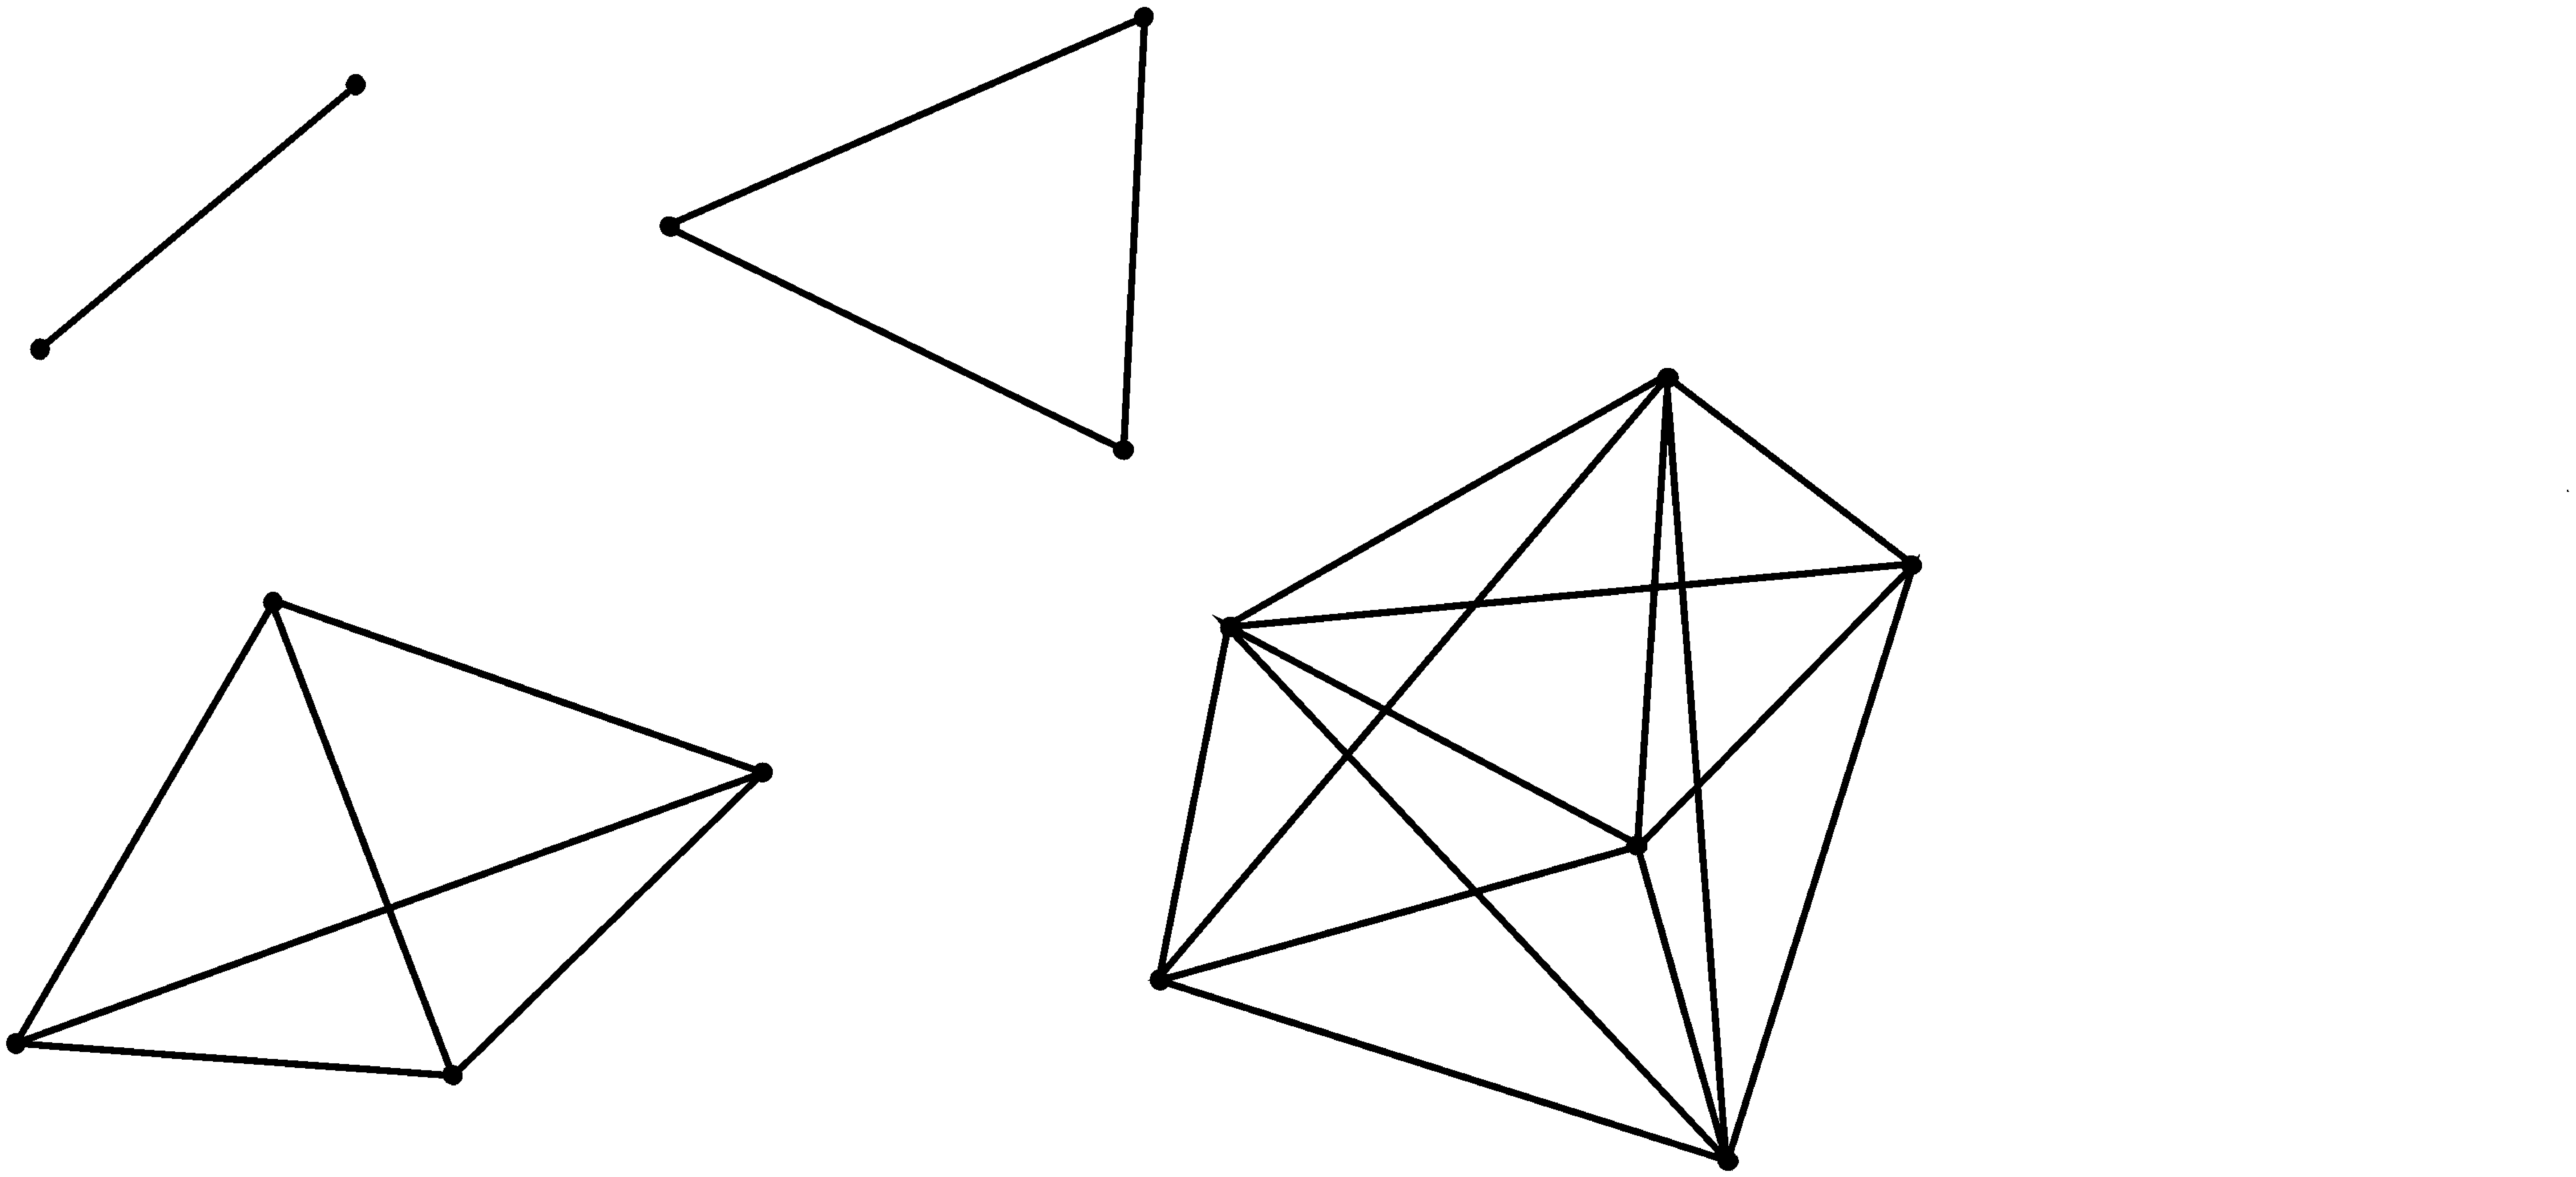
\includegraphics[width=0.6\textwidth]{pict/pict08-2.eps}
\end{center}
 \bigskip
 \refstepcounter{ris}\label{r8-2}

 \centerline{Рис.~\theris}
 \bigskip
\end{figure}

 \vspace{5mm}

Оказывается,
 $$
 \bigcup_{M_n\subset M} \conv M_n=\conv M.
 $$
 Действительно, пусть $x,y$ принадлежат
 $ \bigcup\limits_{M_n\subset M} \conv M_n,$
 тогда $x$ принадлежит некоторому симплексу $\conv M_n,$
 а $y$ принадлежит некоторому симплексу $\conv M_m.$
 Следовательно, $x$ и $y$ принадлежат {симплексу} $\conv M',$ где $M'=M_n
 \bigcup M_m$ и $[x,y]\subset \conv M' \subset
 \bigcup\limits_{M_n\subset M} \conv M_n.$ Таким образом, $\bigcup
 \conv M_n$ выпукло. {Ясно, что это множество} принадлежит любому выпуклому множеству $V,$
 содержащему $M,$ и есть их пересечение.

 \begin{Corollary} %%% Следствие.
 {Множество}
 $$
 \bigcup_{M_n\subset M} \conv M_n
 $$
 есть наименьшее выпуклое множество, содержащее $M.$
 \end{Corollary}

 \begin{Remark} %%% Замечание.
 Если $x_1,\ldots, x_n\subset M,$ то $\conv M_n$ {совпадает с множеством}
 $$
 \left\{x=\sum\limits_{k=1}^n c_kx_k:\quad c_k\ge 0,\quad \sum\limits_{k=1}^n
 c_k=1\right\}.
 $$
 \end{Remark}

Бывает нужна также {\it замкнутая выпуклая оболочка} $\overline{\conv M}$
множества $M.$

\ \

\section{Характеристики линейных нормированных пространств}

{\bf 1.~Сепарабельность}
\vspace{3mm}

Характеристикой массивности пространства является
 наименьшая мощность всюду плотного множества.

 Пространство, для которого существует всюду
 плотное счетное множество, называется {\it сепарабельным}.

 Пространство, не совпадающее с $\theta$ и в котором нет всюду
 плотного счетного множества, называется {\it несепарабельным}.

 Первое, что мы должны проверять для пространства -- сепарабельность.

\vspace{5mm}
{\bf 2.~Полнота}
\vspace{5mm}

Пространство называется {\it полным}, если всякая последовательность
 Коши (фундаментальная последовательность) является сходящейся к
 какому-либо элементу пространства.

 Полное линейное нормированное пространство
 называется {\it банаховым пространством} или пространством
 типа $B.$

\vspace{5mm}
{\bf 3.~Рефлексивность}
\vspace{5mm}

Пусть $X$ -- банахово пространство; $X^*$ -- сопряженное с ним
 пространство линейных непрерывных функционалов, всегда банахово; $X^{**}$ -- второе
 сопряженное пространство.

 Существует каноническое вложение $X$ в $X^{**}$ посредством формулы:
 {для любого} {$x\in X$ положим}
 $$
 F_{{x}}(f)=f(x),\qquad f\in X^*,
 $$
 так что
 $$
 \forall\ x\in X\qquad x\longmapsto F_{{x}}\in X^{**}.
 $$

 Пространство называется {\it рефлексивным}, если при
 каноническом вложении $X$ в $X^{**}$ на самом деле имеем $X\equiv X^{**}$,
 {т.\,е. любой функционал}
 {$F\in X^{**}$ совпадает с некоторым функционалом}
 {$F_x$ над $X^*$.}

 Если пространство рефлексивно, то $X$ и $X^{**}$ устроены одинаково (изоморфны и изометричны).
 Обратно неверно, $X$ и $X^{**}$ могут быть, например, изоморфны, но
 $X$ не рефлексивно.

 Известно, что если  пространство рефлексивно,
 то из любой ограниченной последовательности
 его элементов можно выбрать слабо сходящуюся подпоследовательность.

\vspace{5mm}
 {\bf 4.~Строение сферы (шара)}
 \vspace{5mm}

 {\bf \normalsize   a) Строгая выпуклость.} Пространство называется {\it строго выпуклым},
 если его единичный шар строго выпуклый.

 Единичный шар строго выпуклый, если для любых $x\ne y,$ принадлежащих шару, любая точка
 на интервале $(x,y)$
 лежит строго внутри шара.

 \begin{Example} %%% Пример.
 Круг -- строго выпуклое множество (рис.~8.3), квадрат -- не строго
 выпуклое. Ясно, что если пространство не строго выпуклое,
 то существует гиперплоскость, которая касается единичного
 шара более, чем в одной точке.

 \vspace{0.5cm}
 %%%%%%%%%%%%%%%%%%%%%%%%%%%%%%%%%%%%%%%%%%%%%%%%%%%%%%
 %\hbox to 0.5cm {}{\special{em:graph pict1.pcx}}
 %\vspace{6cm}
 %%%%%%%%%%%%%%%%%%%%%%%%%%%%%%%%%%%%%%%%%%%%%%%%%%%%%%%%%%
 \begin{figure}[ht]
\begin{center}
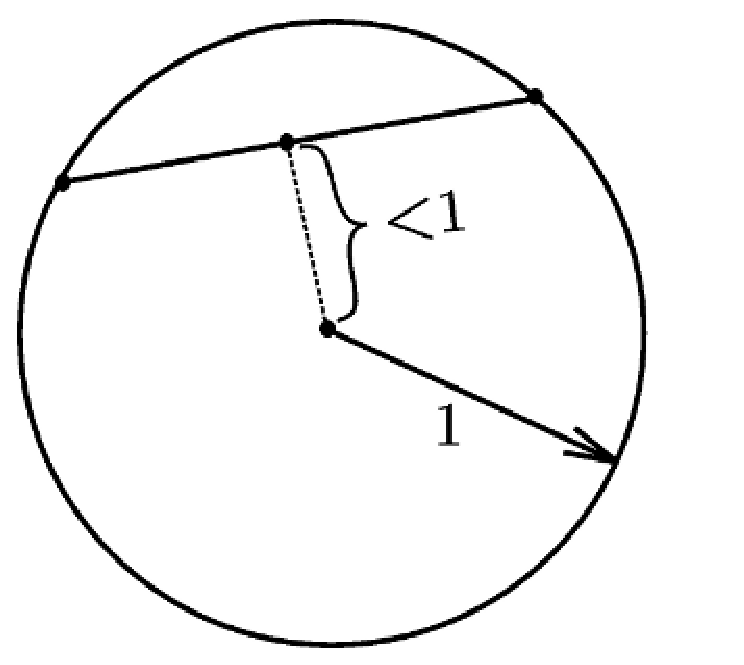
\includegraphics[width=0.3\textwidth]{pict/pict08-3.eps}
\end{center}
 \bigskip
 \refstepcounter{ris}\label{r8-3}

 \centerline{Рис.~\theris}
 \bigskip
\end{figure}
 \end{Example}

 {\bf \normalsize b) Экстремальные точки} {(это линейное понятие).}
 Пусть множество $M\subset X,~ x\in M.$

 Точка $x\in M$ называется {\it неэкстремальной} точкой множества $M,$
 если существуют точки $a,b\in M$ такие, что $x\in (a,b)$
 (рис.~8.4). В противном случае точка называется {\it экстремальной}.

%\newpage

 %\vspace{2cm}
 %%%%%%%%%%%%%%%%%%%%%%%%%%%%%%%%%%%%%%%%%%%%%%%%%%%%%%
 %\hbox to 0.5cm {}{\special{em:graph pict1.pcx}}
 %\vspace{6cm}
 %%%%%%%%%%%%%%%%%%%%%%%%%%%%%%%%%%%%%%%%%%%%%%%%%%%%%%%%%%
   \vspace{10mm}
\begin{figure}[ht]
\begin{center}
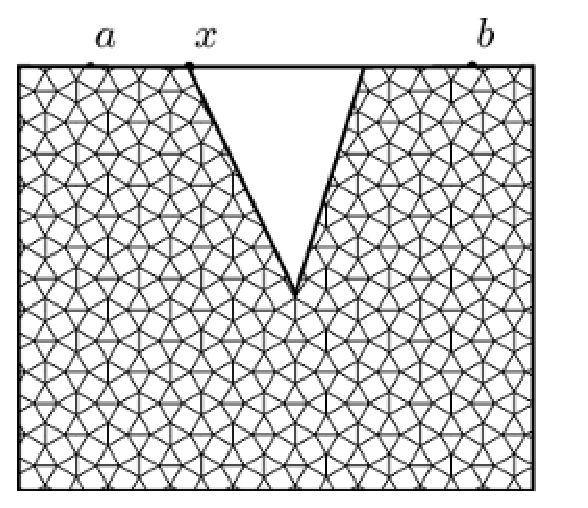
\includegraphics[width=0.3\textwidth]{pict/pict08-4.eps}
\end{center}
 \bigskip
 \refstepcounter{ris}\label{r8-4}

 \centerline{Рис.~\theris}
 \bigskip
\end{figure}

\vspace{5mm}



 Пусть $O_1$ -- единичный шар, $S_1$ -- сфера, его граница.

 {Имеет место}
 \begin{teo}
 В любом конечномерном банаховом пространстве шар $O_1$ есть
 замкнутая выпуклая оболочка своих экстремальных точек.
 \end{teo}

 Теорему приводим без доказательства. В общем случае она неверна. Существуют банаховы
 пространства, в которых единичный шар не имеет
 экстремальных точек.

 \ex
 Доказать, что в единичном шаре $O_1$  в $L{[0,1]}$ нет ни
 одной  экстремальной точки.

 \ex
 Доказать, что шар $O_1$ в $C[0,1]$ имеет две экстремальных точки.

\vspace{5mm}
 {\bf \normalsize c) Гладкость.}
 Пространство называется {\it гладким}, если для любой
 точки на $S_1$ существует единственный опорный функционал,
 т.\,е. единственная касательная гиперплоскости.
 Определение касательной гиперплоскости будет дано позже.

 В противном случае пространство не гладко.

\vspace{5mm}
 {\bf 5.~Компактные множества}
 \vspace{5mm}

  Компактное множество -- такое множество, из любой
 последовательности
 которого можно выбрать сходящуюся подпоследовательность к элементу этого множества.

 Компактное множество всегда замкнуто.

 \vspace{3mm}
 \section{Основные пространства}
  \vspace{3mm}

 {\it Пространство $C=C(Q,X)$ -- это пространство непрерывных функций}, определенных
 на компакте $Q$ и принимающих значения из банахова пространства $X.$
 Классические случаи: $X=\bR,$  $\ X=\bC.$
 \vspace{3mm}

 1. {Пространство $C(Q,X)$} полное.
 \vspace{3mm}

 2. При некоторых $Q$ и $X$ пространство {$C(Q,X)$} сепарабельно, а при некоторых -- нет.

 Если $Q$ -- отрезок, $X=\bR,$ то $C(Q,X)$ сепарабельно.
  \vspace{3mm}

 3. Если $Q$ бесконечно, то $C$ нерефлексивно; в частности, $C[0,1]$ нерефлексивно.
  \vspace{3mm}

 4. {При любых $Q,$ $X$ пространство $C(Q,X)$} не строго выпуклое пространство {и не} {гладкое.}
\vspace{3mm}

 \ex %%%Упражнение.
{Доказать эти свойства.}

{{\it Пространство} $ L^{{p}},~ 1\le p< \infty.$}

 Пусть задано пространство $Q$ с мерой $\mu$ ($\mu$ --
 счетно аддитивная неотрицательная функция измеримых подмножеств из $Q$).

 Пусть $y=f(x)$ -- определенная на $Q$ измеримая
 функция {со значениями в $\bR$ или $\bC$,} для которой
 интеграл  $\ds\int_Q |f(x)|\ d\mu$ конечен, $L_{{\mu}}$ -- множество таких функций и
 $\ds\int_Q |f(x)|\ d\mu=\pnl f\pnr$ -- полунорма.
 Для того, чтобы получить банахово пространство, факторизуем $L_{{\mu}}$:
 $$
  \left. L_{{\mu}} \right/ \{f:\ \pnl f\pnr =0{\}},
  $$
 {т.\,е. будем отождествлять функции, различающиеся лишь на подмножестве нулевой} {меры.}
 Получим полное пространство, которое и далее будем обозначать $L_{{\mu}}.$

 Сепарабельность $L_{{\mu}}$ зависит от $Q$ и от $\mu;$ если $\mu$ --
 мера Лебега на $Q\subset\bR^n,$ то $L_{\mu}=L_{\mu}^1(Q)=L(Q)$ сепарабельно.

 Чтобы получить $L^p_\mu$, возьмем полунорму
 $$
 \pnl f \pnr =\left( \int_Q |f(x)|^p\, d\mu \right)^{1/p}.
 $$
{ Класс эквивалентности, соответствующий функции $f$, будем обозначать тем же}
{символом $f$ и потому $\pnr f\pnr=\|f\|_{L^p}$ -- норма.}

 При $p=2$ получим {$L^2_\mu$} -- гильбертово пространство со скалярным
 произведением
 $$
 (f,g)=\ds\int_Q {fg}\ d\mu
 $$
 над полем действительных чисел,
 $$
 (f,g)=\ds\int_Q {f{\overline g}}\ d\mu
 $$
 над полем комплексных чисел; {$L^2_\mu$}~--
 полное относительно нормы $\|f\|_{{L^2}}=\sqrt{(f,f)}$ {пространство}.

 Напомним, что в пространствах $L^p,\ L^q,$ при $\dfrac{1}{p}+\dfrac{1}{q}=1,\ 1<p,\ q<\infty$
 неравенство Г\"{е}льдера
 $$
 \left| \int_{a}^b f(x)g(x)\,dx\right| \le
 \|f\|_{L^p[a,b]}\|g\|_{L^q[a,b]}
 $$
 для $f\in L^p[a,b],\ g\in L^q[a,b]$ превращается в
 равенство только если $f(x)g(x)\ge 0$ почти всюду и
 $|f(x)|^p$ почти всюду пропорционален $|g(x)|^{q}.$

 \begin{ex}
Рассмотреть эту задачу для функций их $L^p_{\mu}(Q)$ и $L^q_{\mu}(Q).$
 \end{ex}

 % Лекции Сергея Борисовича Стечкина
% ??? Внесены исправления В.И.Бердышева
% Внесены исправления Н.И.Черныха, версия 23.07.2009
% Внесена грамматическая и ТеХ-правка М.Дейкаловой, версия 05.08.09


%%%%%%%%%%%%%%%%%%%%%%%%%%%%%
\chapter{Общие линейные задачи теории приближений}
%%%        Лекция 9.

\section{Выпуклость пространства $L^p$}

Продолжаем рассматривать пространства ${L^p},$~ $1\le p<\infty.$ При $p=2$ пространство
 ${L^2}$ гильбертово. Далее считаем, что $\mu$ -- мера
 Лебега.

Имеет место следующая, приводимая здесь без доказательства
 \begin{teo}    %%% Теорема.
 Полное нормированное пространство {$H$ гильбертово} тогда и только тогда, когда все его
 конечномерные подпространства, включая его, если оно конечномерно,
 евклидовы.
 \end{teo}


 \begin{Corollary} %%% Следствие.
 В гильбертовом пространстве верна плоская геометрия.
 \end{Corollary}

 \begin{Example} %%% Пример.
 Параллелограмм обладает свойством:
  сумма квадратов диагоналей равна сумме квадратов его четырех сторон,
  т.\,е.
 $$
 \|x+y\|^2+\|x-y\|^2=2(\|x\|^2+\|y\|^2)
 $$
 (закон параллелограмма). В курсе анализа
  доказывается, что уже это свойство характеризует гильбертово
  пространство.
 \end{Example}

 При $p\ne 2,$~ $p>1,$ пространство ${L^p}$ (если его размерность больше 1)
 не является гильбертовым,
 но является строго выпуклым и рефлексивным.

 В любом банаховом пространстве норма удовлетворяет  неравенству
 треугольника
 $$
 \|x+y\|\le \|x\|+\|y\|.
 $$
 В ${L^p}$ получаем
 $$
 \left\{ \int_Q {|x+y|}^p\, dt \right\}^{1/p} \le
 \left\{ \int_Q |x|^p\, dt \right\}^{1/p}+
 \left\{ \int_Q |y|^p\, dt \right\}^{1/p}
 $$
 -- классическое неравенство Минковского. Здесь
  равенство (в вещественном случае) будет тогда и только тогда, когда
 $x$ и $y$ положительно пропорциональны, т.\,е. существуют
 $\alpha,\beta \ge 0$ и $\alpha^2+\beta^2>0$ такие, что $\alpha
 x=\beta y,$ т.\,е. $x$ и $y$ лежат на одном луче, исходящем из начала
 (см. условный рис.~9.1).

 Это свойство называется свойством {\it строгой
  нормированности}; оно эквивалентно строгой выпуклости пространства.

  \begin{figure}[ht]
\begin{center}
\includegraphics{pict/pict09-1.eps}
\end{center}
 \bigskip
 \refstepcounter{ris}\label{r9-1}

 \centerline{Рис.~\theris}
 \bigskip
\end{figure}


 Следовательно, для любого $p>1$ пространство ${L^p}$ строго выпукло. Пространство ${L^1}$
 не является строго выпуклым; для обоснования этого построим в ${L^1}[0,1]$
  два элемента $x$ и $y$ таких, что в неравенстве Минковского
  {выполняется равенство}, но $x$ и $y$ не будут положительно пропорциональны:
  {достаточно положить}
  $$
    {
    x(t) = \begin{cases}
      1, & t \in [0,1/2)  \\[7pt]
      0, & t \in [1/2,1]
    \end{cases},\qquad
    y(t) = \begin{cases}
      0, & t \in [0,1/2)  \\[7pt]
      1, & t \in [1/2,1]
    \end{cases}.}
  $$

 % \vspace{1cm}
 %%%%%%%%%%%%%%%%%%%%%%%%%%%%%%%%%%%%%%%%%%%%%%%%%%%%%%
 %\hbox to 0.5cm {}{\special{em:graph pict1.pcx}}
 %\vspace{6cm}
 %%%%%%%%%%%%%%%%%%%%%%%%%%%%%%%%%%%%%%%%%%%%%%%%%%%%%
 На рис.~\ref{r9-2} представлен еще один вариант функций
 $x$ и $y.$

 \bigskip
\begin{figure}[ht]
\begin{center}
\includegraphics{pict/pict09-2.eps}
\end{center}
 \bigskip
 \refstepcounter{ris}\label{r9-2}

 \centerline{Рис.~\theris}
 \bigskip
\end{figure}

 Пример легко распространить на пространства $L_{\mu}.$

 %\bigskip

 \section{Равномерная выпуклость}

 Возьмем единичный шар $O_1$ в банаховом пространстве, проведем гиперплоскость
  на расстоянии $h<1$ от $\Theta_X,$ <<отрежем ломтик>> $l$ от шара $O_1$ (см. рис.~\ref{r9-3}).
   Будем брать $d(l)$
  -- диаметр <<ломтика>>. Теперь устремим $h$ к $1$ и рассмотрим
 $\lim\limits_{h\to 1} d(l).$

 \bigskip
\begin{figure}[ht]
\begin{center}
\includegraphics{pict/pict09-3.eps}
\end{center}
 \bigskip
 \refstepcounter{ris}\label{r9-3}

 \centerline{Рис.~\theris}
 \bigskip
\end{figure}


\noindent В евклидовом пространстве $d(l)\to 0$~ $(h\to 1).$

 Пространство называется {\it равномерно выпуклым}, если
  диаметр $d(l) \rightrightarrows 0$~ $(h\to 1)$
  равномерно по всем гиперплоскостям {(по всем <<ломтикам>>)}.
  Ясно, что равномерно выпуклое пространство -- строго
  выпуклое.

 {Имеет место} следующая теорема, которую также приводим
 без доказательства.
 \begin{teo}[Кларксон] %%% Теорема
 Всякое равномерно выпуклое банахово пространство рефлексивно.
 \end{teo}

 Доказать равномерную выпуклость пространства ${L^p}$ при $p>1,$
 просто, следовательно, ${L^p},$~ $p>1$,  рефлексивно. ${L^1},$
 вообще говоря, не рефлексивно, за исключением
 вырожденных случаев, когда мера сосредоточена в
 конечном числе точек.

 \section{Общие линейные задачи теории приближений}

 {\bf Постановка задачи.} Пусть $X$ -- банахово пространство,
 $L$ -- собственное подпространство $(L\ne X)$ ($L$ замкнуто).

 Рассмотрим задачу о наилучшем приближении
 любого элемента $x\in X$ при помощи элементов $y\in L,$ т.\,е. рассмотрим
 задачу
 $$
 \inf_{y\in L} \|x-y\|_X=E(x,L)_X.
 $$

 \vspace{3mm}
 {\bf 1.~Проблема единственности}
 \vspace{3mm}

 Для любого $x\in X$ составим множество $Y(x)$
 (может быть, и пустое):
 $$
 Y(x)=\{ y^*\in L : \|x-y^*\|_X=E(x,L)_X\}
 $$
 -- множество (или многогранник) наилучших элементов;
 $$
 x\longmapsto Y(x)\subset L.
 $$

Далее исследуется следующая

 \task %%% Задача.
 При каких условиях на $X$ для любого $x\in X$ и любого $L$
 мощность $\mbox{card}\ Y(x)\le 1?$ Т.\,е. для каких $X$
 для любого $x\in X$ в любом подпространстве $L$
 имеется не более одного наилучшего элемента?

\begin{defi}
 Если для любого подпространства $L$ и для любого элемента $x\in X$
 найдется только один или {не найдется} ни одного наилучшего элемента, то будем
 говорить, что $X$ обладает {\it свойством единственности} $(U).$
 \end{defi}

 \begin{teo} %% Теорема.
 Для того чтобы банахово пространство обладало свойством $(U)$,
 необходимо и достаточно, чтобы оно было строго выпуклым.
 \end{teo}

 \begin{proof} %%% Доказательство.
 Д\;о\;с\;т\;а\;т\;о\;ч\;н\;о\;с\;т\;ь.~ Пусть $X$ строго выпукло. Предположим, что
 $(U)$ не выполняется, т.\,е. существуют $L\subset X,$ $x\in
 X$ и $y_1,y_2$ такие, что
 $$
 \{y_1,y_2\}\subset Y_L(x),\qquad y_1\ne y_2.
 $$
 Тогда
 $$
 \inf_{y\in L} \|x-y\|=\|x-y_1\|=\|x-y_2\|=E(x,L)_X>0.
 $$
 Рассмотрим элемент $y=\dfrac{1}{2}(y_1+y_2).$ Подсчитаем уклонение $x$
 от $y$:
 $$
 \|x-y\|=\left\| \frac{1}{2} (x-y_1)+\frac{1}{2}(x-y_2) \right\|.
 $$
 Элемент $x-y$ есть середина отрезка $[x-y_1,x-y_2],$ концы
 которого лежат на сфере $S$ радиуса $\rho=E(x,L)_X.$
 Тогда в силу строгой выпуклости пространства элемент $x-y$
 лежит строго внутри шара ${O}_{\rho},$ значит, имеет строго меньшую норму, т.\,е.
 $$
 E(x,L)_X \le \|x-y\|=\left\| \frac{1}{2}(x-y_1)+\frac{1}{2}(x-y_2)
 \right\|<\|x-y_1\|=\|x-y_2\|=E(x,L)_X
 $$
 -- противоречие.



 {Н\;е\;о\;б\;х\;о\;д\;и\;м\;о\;с\;т\;ь.}~ Пусть $X$ обладает свойством $(U),$
 надо доказать, что тогда $X$ строго выпукло. Предположим, что $X$
 не строго выпукло, тогда существует гиперплоскость $L,$
 расстояние от которой до {начала} $\theta_X$ равно 1 и которая
 касается единичной сферы по крайней мере в двух точках $s_1,s_2.$
 <<Сдвинем>> гиперплоскость так, чтобы $L\to L_1,$~ $\theta_X\to x_0,$~ $L_1$
 -- подпространство, т.\,е. $L_1\ni \theta_X,$ тогда $s_1\to y_1,$~ $s_2\to y_2.$

 \bigskip
\begin{figure}[ht]
\begin{center}
\includegraphics{pict/pict09-4.eps}
\end{center}
 \bigskip
 \refstepcounter{ris}\label{r9-4}

 \centerline{Рис.~\theris}
 \bigskip
\end{figure}


 Рассмотрим элемент $x_0$ (см. рис.~\ref{r9-4}). Для него в подпространстве $L_1$
 есть по крайней мере два элемента наилучшего  приближения $y_1$
 и $y_2.$ Противоречие. Теорема доказана.
 \end{proof}

\begin{Remark} %%% Замечание.
  { Мы фактически доказали, что если $y_1\in Y(x),$~ $y_2\in Y(x),$
 т.\,е.
 $$
 E(x,L)=\|x-y_1\|=\|x-y_2\|,
 $$
 то $[y_1,y_2]\subset Y(x).$}
 \end{Remark}

{ Действительно, любой элемент $y$ из $[y_1,y_2]$
 представляется в виде $y=ty_1+(1-t)y_2$ при некотором $t\in [0,1].$
 Тогда
 $$
{E(x,L)\le} \|x-y\|=\|t(x-y_1)+(1-t)(x-y_2)\|\le t\|x-y_1\|+(1-t)\|x-y_2\|=E(x,L).
 $$}

  \begin{Corollary} %%% Следствие.
 Многогранник наилучших приближений -- всегда выпуклое множество $($и, значит, для
 строго выпуклого пространства он либо пуст, либо состоит
 только из одного элемента$)$.
 \end{Corollary}

 Из классических пространств пространства $C$ и ${L^1}$ не являются строго выпуклыми,
 следовательно, $C$ и ${L^1}$ не обладают свойством единственности.
 {Пространства} ${L^p},$~ $p>1,$ строго выпуклы, следовательно, обладают свойством
 единственности.

 В общем случае все подпространства $\{L\}$ пространства $X$
 делятся на обладающие и  не обладающие свойством единственности.
 {На {рис.~\ref{r9-5}} изображены сфера и два}
 {подпространства пространства на плоскости с нормой,
 определяемой этой сферой.

 \begin{figure}[ht]
\begin{center}
\includegraphics{pict/pict09-5.eps}
\end{center}
 \bigskip
 \refstepcounter{ris}\label{r9-5}

 \centerline{Рис.~\theris}
 \bigskip
\end{figure}


 \vspace{3mm}
 {\bf 2.~Проблема существования}
  \vspace{3mm}

 Если для  любого $x\in X$ в любом подпространстве $L$
 найдется  хотя бы один наилучший элемент, то будем говорить, что $X$
 обладает свойством существования $(E).$

Будем говорить, что гиперплоскость {$L_1$} касается сферы
$S_1$, если существует элемент $y\in S_1=\{ z\in X:\ \|z\|=1\}$
такой, что $\inf\limits_{x\in {L_1}} \|x-y\|=0.$ Заметим, что касание не предполагает наличие точки касания.

Для банаховых пространств {имеет место}
 \begin{teo}[Джеймс] %%% Теорема
 Для того чтобы банахово пространство было рефлексивным, необходимо и
 достаточно, чтобы всякая гиперплоскость этого пространства,
 касающаяся единичной сферы, имела $($хотя бы одну$)$ точку касания
 {или, что то же самое, всякая гиперплоскость $L_x=\{y : f(y)=f(x)\}$ имела бы точку}
 {касания со сферой $S_E=\{z\,:\,\|z\|=E(x,L)\},$ где $L$~-- подпростанство $\{y:f(y)=0\}.$}
 \end{teo}

% \begin{proof} %%% Доказательство.
 Таким образом, пространство $X$
  рефлексивно тогда и только тогда, когда для любого $f\in X^*$
 найдется $x\in X$ такой, что $\|x\|=1$ и $|f(x)|=\|f\|$
 (т.\,е. на элементе $x$ достигается норма функционала).
 %Не ограничивая общности,
 %можно считать, что $\|f\|=1.$ Тогда множество $\{ y : f(y)=1\}$
 %-- гиперплоскость и должен существовать элемент $x,$~ $\|x\|=1$,
 %такой, что $f(x)=1.$
 %\end{proof}

 \begin{Example} %%% Пример.
 В $C[0,1]$ рассмотрим функционал $f(x)=\ds\int_0^1 \sign\sin 2\pi t\cdot
 x(t)\,dt.$ Норма этого функционала
 $$
 \|f\|=\int_0^1 |\sign\sin 2\pi t|\, dt=1,
 $$
 но она не достигается в $C,$ так как функция $x(t)=\mbox{sign} \sin
 2\pi t$ не принадлежит $C[0,1].$


 \noindent В этом примере точки касания гиперплоскости $f(x)=1$ с единичной сферой
 $S_1$ в $C[0,1]$ нет (как легко видеть, для любой $x(t)\in C[0,1],~ \|x\|_C=1,~
 \Longrightarrow |f(x)|<1$).
 \end{Example}

 \begin{teo} %%% Теорема.
 Банахово пространство обладает свойством $(E)$
 в том и только том случае, когда оно рефлексивно.
 \end{teo}

 \begin{proof} %%%Доказательство.
 1) Пусть $X$ не рефлексивно. Тогда по теореме Джеймса существует
 гиперплоскость $\{ f(x)=1\},$ {$\|f\|=1,$} которая не имеет точки касания с
 единичной сферой. Рассмотрим подпространство $L=\{{y}:f(y)=0\}.$
 Тогда для любого элемента $x$ такого, что $f(x)\ne 0$ в $L$
 нет ближайшего элемента (если бы был, то после
 <<сдвига>> получили бы точку касания для гиперплоскости $L_x$ {(см. рис.~9.6)}).

 \vspace{10mm}
 %%%%%%%%%%%%%%%%%%%%%%%%%%%%%%%%%%%%%%%%%%%%%%%%%%%%%%
 %\hbox to 0.5cm {}{\special{em:graph pict1.pcx}}
 %\vspace{6cm}
 %%%%%%%%%%%%%%%%%%%%%%%%%%%%%%%%%%%%%%%%%%%%%%%%%%%%%%%%%%
 %\noindent \hskip3.0cm {рис.}
 %\bigskip
\begin{figure}[ht]
\begin{center}
\includegraphics{pict/pict09-6.eps}
\end{center}
 %\bigskip
 \refstepcounter{ris}\label{r9-6}

 \centerline{Рис.~\theris}
% \bigskip
\end{figure}

 2) Пусть $X$ рефлексивно. Докажем, что тогда оно обладает свойством
 $(E).$ Прежде всего заметим, что если $\{ x_n\}\in L$ и $x_n \dashrightarrow x$
 (слабо сходится к $x$), то $x\in L$ и
 $$
 \|x\|\le d =
 \mathrel{\mathop{\underline{\lim}}\limits_{n\to \infty}} \|x_n\|.
 $$

 Пусть теперь $L$ -- любое подпространство и $x$ -- любой элемент из
 $X,$ {$x\not \in L.$} Построим шары $O_{d+\varepsilon_n}=O_{d+\varepsilon_n}(x)$ (см. рис.~9.7) с центром в $x$
 и радиусом $d+\varepsilon_n,$ где $d=E(x,L)$ и $\varepsilon_n
 \downarrow 0.$ Рассмотрим множества $K_n=O_{d+\varepsilon_n}\cap L.$
 $\{K_n\}$ -- вложенная последовательность непустых ограниченных
 замкнутых множеств.  В рефлексивном пространстве такая последовательность
 имеет непустое пересечение. Действительно, возьмем
 $$
 x_n\in K_n,\qquad \|x-x_n\| \longrightarrow d.
 $$
 Последовательность $\{x-x_n\}$~-- слабо компактная. Известно, что из нее можно
 выбрать подпоследовательность $\{x-x_{n_k}\},$
 слабо сходящуюся к некоторому элементу $x-x_0,\ x_0\in \cap K_n.$ Следовательно,
 $x_0\in L$ и $\|x-x_0\|\le
 d.$ Так как $d=E(x,L),$ то строгого неравенства не может быть, так что, на самом деле
 $\|x-x_0\|=d$ и, значит, $x_0$ -- наилучший элемент. Теорема доказана.
 \end{proof}

 \bigskip
\begin{figure}[ht]
\begin{center}
\includegraphics{pict/pict09-7.eps}
\end{center}
 \bigskip
 \refstepcounter{ris}\label{r9-7}

 \centerline{Рис.~\theris}
 \end{figure}



 \begin{Corollary} %%% Следствие.
 Всякое конечномерное подпространство есть множество существования.
 \end{Corollary}

 \begin{Remark} %%% Замечание.
 Всякое ограниченно компактное
 множество, т.\,е. множество, пересечение которого с любым
 шаром $O_d(x)$ компактно, есть множество существования.
 \end{Remark}

 \begin{Example} %%% Пример
 {(конечно-параметрического множества} не являющегося ограниченно компактным).
 В $C[0,1]$ рассмотрим множество рациональных дробей вида $R_1=\dfrac{a}{b+ct}\in C[0,1].$
 $R_1$ зависит от трех параметров $a,b,c;$ это множество не компактно в $C[0,1]$:
 последовательность $\left\{ \dfrac{1}{1+ct}\right\}$
 {при $c \to 0$}
 сходится на $(0,1]$
 к $0,$ а в точке {$t=0$} принимает значение, равное $1.$

 Пространство ${L^p},~ p>1,$ является и рефлексивным, и строго выпуклым,
 следовательно, в $L_p,~ p>1,$ любое подпространство есть и
 подпространство $(U)$, и подпространство~$(E).$

 Такие подпространства, являющиеся и
 подпространствами единственности, и множествами
 существования, называются {\it чебышевскими}
 подпространствами.
 \end{Example}

 % Лекции Сергея Борисовича Стечкина
% ??? Внесены исправления В.И.Бердышева
% Внесены исправления Н.И.Черныха, версия 23.07.2009
% Внесена грамматическая и ТеХ-правка М.Дейкаловой, версия 05.08.09

%%%%%%%%%%%%%%%%%%%%%%%%%%%%%
\chapter{Критерий наилучшего \\
 приближения в $\boldsymbol L^p$. Корректность}
%%% Лекция 10.


 \section{Критерий наилучшего элемента в $L^p$}

  %%% Замечание.
 Пусть $H$ -- гильбертово пространство. В курсе анализа
 доказывается, что для того чтобы $y^*$ был наилучшим элементом в
 подпространстве
 $M\subset H$ для элемента $x,$ необходимо и достаточно, чтобы
 $$
 (x-y^*,y)=0\qquad \forall\  y\in M.
 $$
 Если $H=L_2,$ то это условие можно переписать
 $$
 \int_Q (x-y^*)y\, dt=0\qquad \forall\  y\in M.
 $$


 Оказывается, это утверждение есть частный
 случай более общей теоремы, которая дает необходимое
 и достаточное условие для наилучшего элемента в $L_p,$~ $p>1.$

 \begin{teo} %%% Теорема.
 Пусть $p>1,$~ $M\subset L_p$ -- подпространство, $ \ x\in L_p.$
 Для того, чтобы $y^*$ был наилучшим элементом из $M$ для $x$
 в $L_p$ необходимо и достаточно, чтобы
 \begin{equation}\label{f9-1}
 {\int_Q |x-y^*|^{p-1} \sign (x-y^*)y\, dt=0} {\qquad \forall\  y\in M}.
 \end{equation}
 \end{teo}

 \begin{proof} %%% Доказательство.
 Н\;е\;о\;б\;х\;о\;д\;и\;м\;о\;с\;т\;ь.~ Пусть условие \eqref{f9-1}
 не выполняется, т.\,е. существует $y\in M$ такой, что
 $$
 {\int_Q |x-y^*|^{p-1} \sign (x-y^*)y\, dt\ne 0.}
 $$
 Покажем, что тогда $y^*$ не есть наилучший элемент.

 Рассмотрим
 $$
 \Phi(\alpha)=\|x-y^*-\alpha y\|^p={\int_Q |x-y^*-\alpha y|^p\, dt.}
 $$
 Так как $p>1,$ то это есть дифференцируемая функция от $\alpha,$
 и по теореме о дифференцировании по параметру под
 знаком интеграла
 $$
 \Phi'(\alpha)=-p {\int_Q |x-y^*-\alpha y|^{p-1}\sign(x-y^*-\alpha y)y\, dt.}
 $$
 При $\alpha=0$ имеем $\Phi'(\alpha)|_{\alpha=0}\ne 0,$
 следовательно, при $\alpha=0$ нет минимума. Значит, при некотором
 $\alpha$ можно сделать уклонение $\|x-y^*-\alpha y\|$ еще меньше, чем
 $\|x-y^*\|,$ т.\,е. $y^*$ не является наилучшим элементом. Противоречие.

 Д\;о\;с\;т\;а\;т\;о\;ч\;н\;о\;с\;т\;ь.~ В силу \eqref{f9-1}, применяя неравенство
 Гельдера,  {для любого} {$y \in M$}
 имеем
 $$
 \int_Q |x-y^*|^{p}\, dt=\int_Q |x-y^*|^{p-1}(x-y^*)\sign(x-y^*)\, dt=
 $$
 $$
 =\int_Q |x-y^*|^{p-1}(x-y)\sign(x-y^*)\, dt \le \int_Q |x-y^*|^{p-1}|x-y|\
 dt\le
 $$
 $$
 \le \left\{ \int_Q |x-y^*|^{p}\, dt \right\}^{1/q}\cdot
 \left\{ \int_Q |x-y|^{p}\, dt \right\}^{1/p},\qquad
 {\frac{1}{p}+\frac{1}{q}=1}.
 $$
 Можно считать, что $\ds\int_Q |x-y^*|^{p}\, dt\ne 0$ (в противном случае
 $y^*$ -- наилучший элемент и все доказано). Тогда
 $$
 \left\{ \int_Q |x-y^*|^{p}\, dt \right\}^{1/p}\le
 \left\{ \int_Q |x-y|^{p}\, dt \right\}^{1/p},
 $$
 т.\,е. для любого $y\in M$ выполняется неравенство $\|x-y^*\|\le \|x-y\|,$ значит,
 $\|x-y^*\|=E(x,M).$
 Теорема доказана.
 \end{proof}

 \begin{Remark} %%% Замечание.
 При $p=1$ {условие} \eqref{f9-1} имеет вид
\begin{equation}\label{f9-2}
 \int_Q \sign(x-y^*)y\, dt=0,\qquad \forall\  y\in M,
\end{equation}
 и это есть достаточное условие для того, чтобы $y^*$
 был наилучшим элементом для $x$ (доказательство то же самое).
 Это условие будет и необходимым, если априори известно, что
 $x(t)-y^*(t)\ne 0$ почти всюду на $Q$ (так как тогда при $\alpha=0$ почти всюду существует
 производная $\dfrac{d}{d\alpha}|x-y^*-\alpha y|\Big|_{\alpha=0}=-y
 \, \sign(x-y^*)$). В общем случае это условие только
 достаточное. Необходимое и достаточное условие можно найти
 в работе\footnote{Kripke~B.R., Rivlin~T.J. Approximations in the metric of $L_1(X,\mu)$ //
 Trans. Amer. Math. Soc. 1965. Vol.~119, \textnumero~1, iss.~7.
 P.~101--122.}.
% {[Kripke, Rivlin]}.}
 \end{Remark}

%\vspace{2mm}

%{\bf 1. Наилучшее приближение.}
\section{Наилучшее приближение в $L^1$}

Мы рассмотрели приближение в {$L^p$ подпространствами $M$} и
 доказали, что при $p>1$ {элемент} $y^*\in M$
 будет наилучшим элементом для $x$ тогда и только тогда, когда
 \begin{equation}\label{f9-1-10}
 \int |x-y^*|^{p-1} \sign (x-y^*)y\, dt=0\qquad \forall\  y\in M.
 \end{equation}

 \begin{Example} %%% Пример.
 Рассмотрим частный случай $M=\{c\}$ --  одномерное подпространство
 констант.

 Пусть $p=2$, {$L^p=L^2[a,b].$} В этом случае условие \eqref{f9-1-10} запишется так:
 $$
 \int_{a}^b\{x(t)-c^*\}\, dt=0,
 $$
 т.\,е. (см. рис.~10.1) $S_+=S_-.$

 %\vspace{2cm}
 %%%%%%%%%%%%%%%%%%%%%%%%%%%%%%%%%%%%%%%%%%%%%%%%%%%%%%
 %\hbox to 0.5cm {}{\special{em:graph pict1.pcx}}
 %\vspace{6cm}
 %%%%%%%%%%%%%%%%%%%%%%%%%%%%%%%%%%%%%%%%%%%%%%%%%%%%%%%%%%
 %\noindent \hskip3.0cm {рис.}

  \bigskip
\begin{figure}[ht]
\begin{center}
\includegraphics{pict/pict10-1.eps}
\end{center}
 \bigskip
 \refstepcounter{ris}\label{r10-1}

 \centerline{Рис.~\theris}
 \bigskip
\end{figure}



 \noindent Если $p=1,$ то условие \eqref{f9-1-10} перепишется как
 $$
 \int_a^b\sign \{x(t)-c^*\}\, dt=0
 $$
 или, { в случае, когда $L^1[a,b]$ есть пространство с мерой $\mu,$ как}
 \begin{equation}\label{f10-1}
 \mu(E_+)-\mu(E_-)=0,
 \end{equation}
 где $E_+\ (E_-)$ -- множество, на котором разность $x(t)-c^*>0\
 (<0),$~ $\mu$ -- мера.
 \end{Example}

 Легко построить пример, когда нет единственности
 наилучшего элемента в {$L^1$} \linebreak {{(см. рис.~10.2)}:}

\begin{figure}[ht]
\begin{center}
\includegraphics[width=0.5\textwidth]{pict/pict10-2.eps}
\end{center}
 \bigskip
 \refstepcounter{ris}\label{r10-2}

 \centerline{Рис.~\theris\ \  $(c^*\in [0,1])$}
\end{figure}



 \noindent Любая константа $c^*\in [0,1]$ -- {здесь} наилучшая.

 Как отмечалось, при $p=1$ {условие} \eqref{f9-1-10} -- {только} достаточное для наилучшего
 элемента. Можно построить пример, когда для наилучшей
 константы в {пространстве $L^1$ с мерой} условие \eqref{f10-1} {тоже} не выполняется
 (см. рис.~10.3 для меры Лебега).

 %\vspace{2cm}
 %%%%%%%%%%%%%%%%%%%%%%%%%%%%%%%%%%%%%%%%%%%%%%%%%%%%%%
 %\hbox to 0.5cm {}{\special{em:graph pict1.pcx}}
 %\vspace{6cm}
 %%%%%%%%%%%%%%%%%%%%%%%%%%%%%%%%%%%%%%%%%%%%%%%%%%%%%%%%%%
 %\noindent \hskip3.0cm {рис.}
 \bigskip
\begin{figure}[ht]
\begin{center}
\includegraphics{pict/pict10-3.eps}
\end{center}
 \bigskip
 \refstepcounter{ris}\label{r10-3}

 \centerline{Рис.~\theris\ (здесь видно, что $c^*=1/2$)}
 \bigskip
\end{figure}




 Если {же $\mu\{t\in[a,b] : x(t)-y^*(t)=0\}=0,$} то дифференцирование под знаком интеграла
 законно, и нарушение условия \eqref{f10-1} означает, что $y^*$ не является наилучшим
 элементов в $M$ для $x$.

 Пусть $X$ -- банахово пространство, $M\subset X $ --
 подпространство.
 В задаче о наилучшем приближении для любого $x\in X$
 мы ищем $y^*\in M$ такой, что
 $$
 \|x-y^*\|_X\le \|x-y^*-h\|\qquad \forall\  h\in M;
 $$
 т.\,е. $y^*$ будет наилучшим элементом, если  не найдется понижающий
 элемент $h.$ Значит, функционал
 $$
 \Phi(h)=\|x-y^*-h\|
 $$
 должен достигать при $h=\theta$ своего минимума. Если $\Phi(h)$ --
 дифференцируемый функционал, то для минимума необходимо, чтобы
 дифференциал от $\Phi(h)$ обращался в 0 при $h=\theta.$
 Или пусть фиксировано $h.$ Тогда функционал
 $$
 F_h(t)=\|x-y^*-th\|,\qquad t\in (-1,1),
 $$
 должен иметь минимум в точке $t=0$ при каждом $h\in M$; т.\,е. $\cD\|x-y^*-h\|
 |_{h=\theta}=0,$ так что условие \eqref{f9-1-10} просто означает, что дифференциал равен
 нулю.

 Так как $\Phi(h)$ -- выпуклый функционал, то
если $\Phi(h)$~-- дифференцируемый функционал,
 условие обращения дифференциала для $\Phi(h)=\|x-y^*-h\|$ на пространстве
 $M$ в 0 при $h=\theta$ есть необходимое и достаточное для того, чтобы $y^*$
 был наилучшим.

\section{Корректность}

Рассмотрим вопрос о непрерывной зависимости решения задачи наилучшего приближения
от задаваемых условий.

 Пусть $X$ --~банахово пространство, и пусть далее $M\subset X$ --~множество
 существования, элементы $x\in X,$ $y(x)$ -- элемент
 наилучшего приближения в $M$ для $x$, $E(x,M)_X$ --~наилучшее приближение
 элемента $x.$ Очевидно, что $E(x,M)_X=\Phi(x)$ --
 функционал~от~$x.$

 Так как
 $$
 E(x,M)-E(x',M)=\|x-y(x)\|-\|x'-y(x')\|\le \|x-y(x')\|-\|x'-y(x')\|\le
 \|x-x'\|,
 $$
 то получаем, что {\it наилучшее приближение {$E(x,M)$} зависит от} $x$
 {\it {непрерывно и} {даже равномерно непрерывно.}}

\ex Доказать полученную оценку без предположения $M\in (E).$

 Пусть теперь в $M$ и для $x$, и для $x'$ существуют единственные
 наилучшие элементы $y(x)$ и $y(x').$ Если $x$ и $x'$ близки,
 следует ли тогда, что $y(x)$ и $y(x')$ близки? Вообще говоря, это не
 так, $y(x),$ вообще говоря, не является непрерывной функцией от $x.$
 Но непрерывность $y(x)$ имеет место в одном важном случае.

 Пусть $M$ ограниченно компактно, т.\,е. пересечение $M$
 с любым шаром {есть} компакт. Ограниченно компактное
 множество всегда есть множество существования, т.\,е.
 для любого $x$ множество наилучших элементов
 $Y(x)\subset M$ не пусто. {Нас интересует} {непрерывность отображения}
 $$
   x \longmapsto Y(x)\subset M,\qquad{ x \in X}.
 $$
 Будем рассматривать {$Y_{\varepsilon}$~--} $\varepsilon$-расширение $Y(x)$ в $M$,~
 {$Y_{\varepsilon}=\{y\in M:\rho(y,Y(x))<\varepsilon\}$}
 Зафиксируем какой-нибудь элемент $x\in X.$
 Выясним, как связаны $Y_{\varepsilon}$ и $Y.$

 %\vspace{2cm}
 %%%%%%%%%%%%%%%%%%%%%%%%%%%%%%%%%%%%%%%%%%%%%%%%%%%%%%
 %\hbox to 0.5cm {}{\special{em:graph pict1.pcx}}
 %\vspace{6cm}
 %%%%%%%%%%%%%%%%%%%%%%%%%%%%%%%%%%%%%%%%%%%%%%%%%%%%%%%%%%
 %\noindent \hskip3.0cm {рис.}

  \bigskip
\begin{figure}[ht]
\begin{center}
\includegraphics{pict/pict10-4.eps}
\end{center}
 \bigskip
 \refstepcounter{ris}\label{r10-4}

 \centerline{Рис.~\theris}
 \bigskip
\end{figure}



 \noindent Ясно, что $Y=\bigcap\limits_{\varepsilon >0} Y_{\varepsilon}.$
 Теперь возьмем $E(x,M)=d$ и рассмотрим множество\linebreak (см. рис.~10.4)
 $$
 Z(\varepsilon)=Z(\varepsilon,x)=\{ z\in M:\ \|x-z\|\le d+\varepsilon\}.
 $$
 Тогда для ограниченно компактных множеств $M$ справедливо

 \begin{Proposition} %%% Утверждение.
 Для любого $\varepsilon>0$ найдется $\varepsilon_1>0$ такое, что
 $Z(\varepsilon_1)\subset Y_\varepsilon.$
 \end{Proposition}

 Действительно, {$\{Z(\varepsilon_1)\}_{\varepsilon_1}$} --
 убывающая по вложению при $\varepsilon_1\downarrow 0$
 система компактных множеств и $\bigcap\limits_{\varepsilon_1>0} Z(\varepsilon_1)=Y{(x)}.$
 Тогда по свойству компактных множеств для любой окрестности
 $Y_{\varepsilon}$  {множества $Y(x)$}
 все $Z(\varepsilon_1),$ начиная
 с некоторого $\varepsilon_0,$ т.\,е. при $\varepsilon_1\le \varepsilon_0,$
 лежат внутри $Y_{\varepsilon}.$

 В общем случае, если нет ограниченной компактности, это утверждение
 не имеет места.

 В частности получаем, что если
 {в ограниченно компактном множестве $M$}
 есть единственный
 наилучший элемент
{для $x$}, то все <<хорошие>> точки, т.\,е. такие $z\in M,$
 расстояние от которых до $x$
 мало отличается от наилучшего приближения, лежат
 в некоторой малой окрестности наилучшего элемента.

 \begin{teo}[о корректности] %%% Теорема
 Пусть $X$ -- банахово пространство, $M$ -- ограниченно компактное
 подмножество из $X,$~ $x\in X$ и существует единственный элемент
 $y^*\in M,$ ближайший к {$x.$} Тогда если $\{x_n\}$ -- любая сходящаяся
 к $x$ последовательность из $X$ и $\{y_n\}$ -- последовательность из
 $M$ такая, что $\|x_n-y_n\|\to \|x-y^*\|,$ то $y_n\to y^*.$
 \end{teo}

 Действительно, для любого $\delta>0$ для достаточно
 больших $n$
 $$
 \|x-y_n\|\le \|x-x_n\|+\|x_n-y_n\|\le \|x-y^*\|+\delta,
 $$
 т.\,е. $y_n\in Z(\delta).$ Мы уже отмечали, что для любого
 $\varepsilon>0$ множество $Z(\delta)$ принадлежит $Y_{\varepsilon}$ для
 достаточно малых $\delta.$ Таким образом, $\|y_n-y^*\|\le \varepsilon$
 для всех достаточно больших $n,$ т.\,е. $y_n\to y^*.$

 Учитывая непрерывность $E(x,M)$ {получаем}
 \begin{Corollary}
 Пусть $M$ -- ограниченно компактное множество из $X$
 и для любого $x\in X$ наилучший элемент $y(x)$ -- единственный.
 Тогда $y(x)$ {есть} непрерывная функция от $x$
 на всем банаховом пространстве. {При этом} $y(x)$ будет равномерно непрерывной
 функцией, если $x\in K,$ где $K$ -- компакт.
 \end{Corollary}

 \task %%% Задача.
 В пространстве $C{=C[0,1]}$ приближаем функциями из класса
 $$
 \{ x\in C:\quad \|x'\|\le 1,\quad x(0)=0\}.
 $$
 Будет ли $y(x)$ непрерывна? В каких банаховых пространствах для
 любого подпространства {$M$ метрическая проекция $y(x)$}
 равномерно непрерывна?

 Пусть $H$ -- гильбертово пространство, $M\subset H $ -- подпространство,
 $  x\in X,$ $y(x)$~{-- ближайший к $x$ элемент в $M.$}
 Из критерия наилучшего приближения
 $$
 (x-y(x),y)=0\qquad \forall\  y\in M
 $$
 следует, что
 $$
 \|x-y(x)\|^{2}+\|y(x)\|^2=\|x\|^2
 $$
 и
 $$
 \|y(x)\|\le \|x\|.
 $$
 Тогда {в силу линейности метрической проекции в $H$ на подпространство}
 $$
 \|y(x)-y(x')\|=\|y(x-x')\|\le \|x-x'\|,
 $$
 т.\,е. метрическая проекция в гильбертовом
 пространстве равномерно непрерывна (и является
 ограниченным линейным оператором).

 \begin{Remark} %% Замечание.
 Вообще говоря (и как правило, если пространство не гильбертово), линейность наилучших
 элементов не имеет места. Например, пусть в $C[-1,1]$
 приближаем константами {(см. рис.~10.5)} функции
 $$
     {f_1(t)=\begin{cases}
     0, & -1 \le t \le 0 \\
     t, & 0 < t \le 1
   \end{cases},}
   $$
   $$
   f_2(t)=f_1(-t),
   \qquad (f_1+f_2)(t)=|t|.
 $$

 %\vspace{2cm}
 %%%%%%%%%%%%%%%%%%%%%%%%%%%%%%%%%%%%%%%%%%%%%%%%%%%%%%
 %\hbox to 0.5cm {}{\special{em:graph pict1.pcx}}
 %\vspace{6cm}
 %%%%%%%%%%%%%%%%%%%%%%%%%%%%%%%%%%%%%%%%%%%%%%%%%%%%%%%%%%
 %\noindent \hskip3.0cm {рис.}

 \bigskip
\begin{figure}[ht]
\begin{center}
\includegraphics{pict/pict10-5.eps}
\end{center}
 \bigskip
 \refstepcounter{ris}\label{r10-5}

 \centerline{Рис.~\theris}
 \bigskip
\end{figure}

 \noindent Здесь имеем: $\dfrac12=c^*(f_1)=c^*(f_2)=c^*(f_1+f_2)\ne c^*(f_1)+
 c^*(f_2)=1.$

 Линейность имеет место только в гильбертовом
 и некоторых вырожденных пространствах.
 \end{Remark}

 \begin{teo} %%% Теорема.
 Пусть $X$ -- равномерно выпуклое пространство, $M\subset X $ -- подпространство. Тогда $M$
 -- подпространство единственности, и метрическая проекция $y(x)$ {на $M$}
 равномерно непрерывно зависит от $x$ {на любом ограниченном} {множестве}.
 \end{teo}

 \begin{proof} %%% Доказательство.
 Первое утверждение теоремы вытекает из теоремы~9.3.
 Применяя неравенство треугольника
 и используя свойства наилучшего приближения, для произвольных элементов $x$ и $x',$
 обладающих наилучшими элементами в $M,$ получаем
 $$
 \|x-y(x{'})\|\le \|x'-y(x')\|+\|x-x'\|\le \|x'-y(x)\|+\|x-x'\|\le
 $$
 $$
 \le \|x-y(x)\|+\|x-x'\|+\|x-x'\|=\|x-y(x)\|+2\|x-x'\|,
 $$
 т.\,е. если $x'$ близок к $x,$ то равномерно относительно $x$ и $x'$ элемент
 $y(x')$ имеет отклонение от $x$, {близкое к наилучшему.} Получили, что
 $y(x')\in Z(2\|x-x'\|,x).$
 Ввиду равномерной выпуклости пространства отсюда
 следует, что расстояние между $y(x)$ и $y(x')$
 равномерно уменьшается с уменьшением расстояния между $x$ и $x'$
при условии, что величины $\|x\|$ ограничены.

 Пространства $L_p,~ p>1,$ равномерно выпуклы, следовательно, в $L_p,~
 p>1,$
 {на} {ограниченном множестве элементов метрическая проекция}
 $y(x)$ равномерно непрерывна.

 В гильбертовом пространстве, как уже отмечали,
 метрическая проекция равномерно непрерывна {на всем пространстве}.

 В пространстве $C{[a,b]}$ метрическая проекция не является равномерно
 непрерывной.
 \end{proof}

 \begin{Example} %%% Пример.
 В $C[0,1]$ приближаем функциями $a+bx=p(x).$ Построим для любого
 $\varepsilon>0$ непрерывные на $[0,1]$ функции $f$ и $\widetilde f$
 такие, что $\|f-{\widetilde f}\|_C\le \varepsilon,$ но
 $\|p^*(f)-p^*({\widetilde f})\| {> 1}.$
 Это и будет означать, что для метрической проекции $p(f)$
 нет равномерной непрерывности. Пример называется <<молния>> (см. рис.~10.6).
 Здесь $\widetilde f(\varepsilon)=1+\varepsilon,~ \widetilde f(-\varepsilon)=1-\varepsilon,$
 $f(-1)=\widetilde{f}(-1)=0,\ f(1)=\widetilde{f}(1)=0,\ f(0)=\widetilde{f}(0)=-1,\
 f(\varepsilon)=f(-\varepsilon)=1,\ \widetilde{f}(-\varepsilon)=1-\varepsilon,\
 \widetilde{f}(\varepsilon)=1+\varepsilon$~-- вершины
 ломанных -- графиков функций $f(x)$ и $\widetilde{f}(x).$

 %\vspace{2cm}
 %%%%%%%%%%%%%%%%%%%%%%%%%%%%%%%%%%%%%%%%%%%%%%%%%%%%%%
 %\hbox to 0.5cm {}{\special{em:graph pict1.pcx}}
 %\vspace{6cm}
 %%%%%%%%%%%%%%%%%%%%%%%%%%%%%%%%%%%%%%%%%%%%%%%%%%%%%%%%%%
 %\noindent \hskip3.0cm {рис.}

 \bigskip
\begin{figure}[ht]
\begin{center}
\includegraphics{pict/pict10-6.eps}
\end{center}
 \bigskip
 \refstepcounter{ris}\label{r10-6}

 \centerline{Рис.~\theris}
 \bigskip
\end{figure}


 \noindent Здесь наилучшим для $f$ является $p^*(f)\equiv 0,$
 наилучшим для $\widetilde f$ является $p^*(\widetilde f\,)=x,$
 это следует из теоремы Чебышева об альтернансе
 (будет доказана). В примере есть чебышевские
 альтернансы необходимой длины.
 \end{Example}

 \begin{Example} %%% Пример.
В $C[0,1]$ будем приближать функции рациональными дробями из множества
 $$
 M=\left\{ \frac{a}{b+cx}\right\}
 $$
 Можно показать, что оператор наилучшего приближения в этом случае не является непрерывным.

 Действительно, используя критерий Чебышева, для каждого $r>0$ легко построить
 непрерывную функцию $f_r,$ для которой $\dfrac{1}{1+rx}$
 будет наилучшей рациональной дробью (по чебышевскому
 альтернансу в трех точках)
 и такую, что $f_r(x) \rightrightarrows f,$ причем
 для $f$ наилучшая рациональная дробь тождественно равна $0,$ а $\dfrac{1}{1+rx}
 \not\rightrightarrows 0$~ $(r\to \infty),$ так как
 функция $R(x),$ предельная для последней дроби, является разрывной на
 отрезке $[0,1]$: $R(0)=1,\ R(x)=0,\ 0< x\le 1.$

 Таким образом, оператор {наилучшего} проектирования в $C[0,1]$ на {множество} гипербол терпит
 разрыв (см. рис.~\ref{r10-7}).
 \end{Example}

 %\vspace{-5cm}
\begin{figure}[h]
\begin{center}
\includegraphics[width=0.5\textwidth]{pict/pict10-7.eps}
\end{center}
\bigskip
\refstepcounter{ris}\label{r10-7}

\centerline{Рис.~\theris}
\end{figure}

\begin{ex}
 Придумать метрику в трехмерном пространстве (<<шар>>, определяющий
 метрику) такую, чтобы метрическая проекция на некоторое
 одномерное подпространство была разрывной.
\end{ex}

 % ���樨 ��ࣥ� ���ᮢ�� ��窨��
% ���ᥭ� ��ࠢ����� �.�. ����� � �.�. ���쪮��, ����� 24.02.2009
% ���ᥭ� ��ࠢ����� �.�. �����, ����� 16.07.2009
% ���ᥭ� �ࠬ����᪠� � ���-�ࠢ�� �.����������, ����� 05.08.09

\chapter{���பᨬ�⨢��� ������⭮���. �ਡ������� � \boldmath $C$}

\section{�����뢭���� �����᪮� �஥�樨}

����� {$X$ -- �����᪮� ����࠭�⢮,} $M\subset X$,\  $x\in X$,
$Y(x)$~-- ������⢮ �������� ������⮢ ��� $x$ {� $M$}. �᫨ $M$~--
祡�襢᪮� ������⢮, �.\,�. ��� ��� $x$ ������� � ��⮬ �����⢥���
������訩 ������� {$y(x)$}, � �᫨ $M$ �� � ��࠭�祭�� ������⭮� ������⢮,
� �����᪠� �஥���
$$
x\longmapsto Y(x)=\{y(x)\}
$$
�����뢭� (�뫮 ��������).

����� $X$~-- ����客� ����࠭�⢮, $M\subset X$. ������⢮ $M$
���뢠���� \textit{���பᨬ�⨢�� ��������} (�.\,�.), �᫨ ��� ������� $x\in
X$ �� ������������� ��᫥����⥫쭮��� ������⮢ $\{y_n\}$,
�.\,�. ⠪��, �� $y_n\in M$ � $\|x-y_n\|\to E(x,M)_X$~ ($n\to\infty)$, ᮤ�ন�
�����᫥����⥫쭮���, �室������ � �������� �� $M$.

�᫨ ������⢮ $M$ �.\,�. � $Y(x)$ ��⮨� �� ����� �窨, � ��猪�
������������� ��᫥����⥫쭮��� $\{y_n\}$ �室���� � �⮩ �窥.
�⬥⨬ ⠪��, �� �� ���பᨬ�⨢�� ������⭮� ������⢮
�������.

\begin{Example}
�᫨ $H$~-- ��᪮��筮��୮� ���졥�⮢� ����࠭�⢮, � �����筠�
��� $S_1=\{x\colon\|x\|=1\}$ �� ���� ���பᨬ�⨢��
������⭮�, � ������⢮ $M=S_1\cup\{0\}$ ���பᨬ�⨢�� ������⭮.
\begin{figure}[ht]
\begin{center}
\includegraphics[width=0.35\textwidth]{pict/pict11-1.eps}
\end{center}
 \bigskip
 \refstepcounter{ris}\label{r11-1}

 \centerline{���.~\theris}
\end{figure}
\end{Example}

���᭨�, ��� ���஥�� ���பᨬ�⨢�� ������⭮� ������⢮.

\begin{enumerate}
\item �᫨ $M$~-- �.\,�., � $Y(x)\ne \varnothing$ ��� ��� $x\in X$.
\item ��� ��� $x\in X$ ������⢮ $Y(x)$ � �.\,�. ������⢥ $M$ ����
��������, ⠪ ��� ��猪� ��᫥����⥫쭮��� �� $Y(x)$ ����
�����������饩 �, ᫥����⥫쭮, ᮤ�ন� �室������ �����᫥����⥫쭮���.
\end{enumerate}

\begin{teo}[�.\,������]
����� $M$~-- �.\,�. ������⢮ � ����� ��� ������� $x_0$ ������� �����⢥���
������訩 ������� $y(x_0)$. ����� {�����᪠� �஥���
$Y(x)$} �����뢭� � �窥 $x_0$, �.\,�. ��� �� ��᫥����⥫쭮��
$\{x_n\}\to x_0$~ $(n\to\infty)$ � ��� ���� $y_n\in Y(x_n)$ �����
$y_n\to y(x_0)$~ $(n\to\infty)$.
\end{teo}

����⢨⥫쭮, ����� ��᫥����⥫쭮��� $\{x_n\}$
�室���� � $x_0$. ���쬥� �� $y_n\in Y(x_n)$. ����� $\{y_n\}$
�㤥� �����������饩 ��᫥����⥫쭮���� ��� $x_0$, ���
$$
\|x_0-y_n\| = \|x_0-x_n+x_n-y_n\| \le \|x_0-x_n\| + \|x_n-y_n\| =
\|x_0-x_n\| + E(x_n,M) \to E(x_0,M)
$$
�� $n\to\infty$; ᫥����⥫쭮, $y_n\to y(x_0)$~ ($n\to\infty)$.

\begin{Corollary}
�᫨ $M$~-- 祡�襢᪮� �.\,�. ������⢮, � �����᪠� �஥���
$y(x)$ �����뢭� � �� �窥 ����࠭�⢠ $X$.
\end{Corollary}

\begin{Remark}
�⬥⨬ �� ���� ����� ��砩 �����뢭��� �⮡ࠦ���� $Y(x)$. �����
$X$~-- ����客� ����࠭�⢮, $M$~-- ����௫�᪮���. ���
��࠭�祭�� ��魮�� ����� �����, �� $M$ ᮤ�ন� $0$.
{����� �� ����� ������� $x_0 \in X \setminus M$.}
� �⮬
��砥 �� ������� $x\in X$ �।�⠢�� �����⢥��� ��ࠧ�� � ����
$$
x = y+\alpha x_0,\qquad y\in M,\qquad \alpha\in \mathbb R.
$$
{��� ᫥���, �� $Y(x)=y+\alpha Y(x_0)$. ���⮬� �᫨} ��� �����ண�
{$x_0\in X,$} {$x_0\notin M$}, ������訩 �������
{$Y(x_0)$} ������� � �����⢥���, � � ��� ��� {$x\in X$} ������� $Y(x)$
�������, �����⢥��� � �����뢭� ������ �� $x$. �����
�����뢭���� ����� ���� ���� ����� ��������� ����樨 �஥��஢����:
$$
Y(\alpha x_1+\beta x_2)=\alpha Y(x_1)+\beta Y(x_2),\qquad \|Y(x)\| \le 2\|x\|.
$$
\end{Remark}

�������� �ਢ����� 祡�襢᪨� ������⢠, ��騥�� � ⮬� ��
���பᨬ�⨢�� �������묨. �� �� ����࠭�⢮ � �������� ������⢠.

\begin{Remark}
�������� ⠪�� ��᪮��筮���� ����客� ����࠭�⢠, � ������ ���
�� ������ ���ਢ���쭮�� 祡�襢᪮�� �������࠭�⢠ (�ਬ��
�.\,�.\,��ઠ��).
\end{Remark}

\begin{task}
��୮ ��, �� �� ��类� ᥯�ࠡ��쭮� ����࠭�⢥ ࠧ��୮�� ����� 1
�������� ���ਢ����� 祡�襢᪨� �������࠭�⢠?
\end{task}

� $C[0,1]$ ���� ���ਢ����� 祡�襢᪨� �������࠭�⢠, ���ਬ��,
�������࠭�⢮ ����⠭�.

� $L[0,1]$ ⮦� ���� ���ਢ����� 祡�襢᪨� �������࠭�⢠.

\begin{Example}
���ᬮ�ਬ $L(0,1)$, $\|f\|=\ds\int_0^1 |f(t)|\,dt$,
$$
M=\left\{\varphi\in L(0,1)\colon \varphi(t)=0\quad\forall\, t\in [0,1/2]\right\}.
$$

 \bigskip
\begin{figure}[ht]
\begin{center}
\includegraphics{pict/pict11-2.eps}
\end{center}
 \bigskip
 \refstepcounter{ris}\label{r11-2}

 \centerline{���.~\theris}
 \bigskip
\end{figure}

\noindent �� ��.~\ref{r11-2}\ \ $\varphi^*$~-- �����⢥��� ������訩 �������
��� $f \in L(0,1).$
\end{Example}

\begin{task}
�������, �� �� ����筮��୮� ����࠭�⢮ ������⥫쭮�
ࠧ��୮�� ᮤ�ন� 祡�襢᪮� ����௮�����࠭�⢮.
\end{task}

\begin{Remark}
� �� ����筮��୮� ����࠭�⢥ ������� 祡�襢᪮� �������࠭�⢮
�� ����襩 ࠧ��୮�� (�.\,�.\,���������).
\end{Remark}


\section{�ਡ������� � ����࠭�⢥ $C_{2\pi}$}

������ ��宦����� ������襣� ������� �����쭮 ᫮����. ���⮬�
��⠥� ����� �� �業�� ������襣� �ਡ������� $E(f,M)$. ���筮
������ �業�� $E(f,M)$ ������� �� ��ࠢ���⢠
$E(f,M) \le \|f-\varphi\|$, ��ࠢ ���室���� �㭪�� $\varphi\in
M$.

�ਢ���� ��᪮�쪮 �ਬ�஢ �業�� ��� ���� {$C_{2\pi}$}~--
����࠭�⢠ �����뢭�� $2\pi$-��ਮ���᪨� �㭪権 � {$M=\mathcal T_n$}~--
������⢠ �ਣ��������᪨� ��������� �⥯��� �� ��� $n$.

\begin{enumerate}
\item ����� �㭪�� {$f\in C_{2\pi}$} � $\sum\limits_{k=0}^\infty A_k(x)$~--
�� �� ����, ���
$$
A_0(x)=\frac{a_0}{2},\qquad A_k(x)=a_k\cos kx+b_k\sin kx.
$$
�����⭮, �� ������襥 �ਡ������� � ��᫥ �।���� ������筮��
�����⢫���� ���筮� �㬬�� $s_n$ �鸞 ����:
$$
\sum\limits_{k=n+1}^{\infty} (a_k^2+b_k^2) = \frac{1}{\pi} \int_{-\pi}^{\pi}
(f-s_n)^2\, dx\le \frac{1}{\pi} \int_{-\pi}^{\pi}(f-t_n)^2\, dx\le
2\|f-t_n\|^2_C,
$$
��� $t_n\in \mathcal{T}_n$~-- �ந������ �ਣ��������᪨� �������. �������⥫쭮,
$$
E(f,\mathcal T_n)_C\ge \frac{1}{\sqrt{2}}\left( \sum\limits_{k=n+1}^{\infty}
(a_k^2+b_k^2) \right)^{1/2}.
$$

\item ��� �㬬 ����� ���ᥭ� $\sigma_{2n,n}(x)$, �ᯮ���� ��ࠢ���⢮ ������, ����砥�
$$
E(f,\mathcal T_{2n})_C\le \|\sigma_{2n,n}(x)-f\|_C\le \frac{2(2n+1)}{2n-n+1}
E(f,\mathcal{T}_n)_C\le 4E(f,\mathcal{T}_n)_C.
$$
��� ��, �᫨ ����� �ਡ������� �㭪樨 � ������� �㬬 ����� ���ᥭ�
(� ��~-- ����� �����, ⠪ ��� $\sigma_{2n,n}$~-- ������� ������), �
����� �業��� ������訥 �ਡ������� � ᢥ���, � ᭨��.

\item ��� �㬬 ���� ������� �業��
$$
\|f-s_n\|_C\le \left\{ \frac{4}{\pi^2} \ln n+O(1)\right\} E(f,\mathcal{T}_n)_C.
$$
\end{enumerate}


\section{�ਡ������� �樮����묨 �஡ﬨ}

����� $R_{m,n}=R_{m,n}[a,b]$~-- ������⢮ ��� �����ࠨ�᪨� �஡��
���� $R(x)=P(x)/Q(x)$, $\deg P\le m$, $\deg Q\le n,$
��।������� ���� �� ��१�� $[a,b]$.

�㤥� �ਡ������ �㭪�� $f\in C[a,b]$ �樮����묨 �஡ﬨ $R\in
R_{m,n}$. �業�� ����稭� ������襣� �ਡ�������
$$
\inf_{R\in R_{m,n}} \|f-R\|_C=\rho_{m,n}(f).
$$

�㤥� �।��������, �� �஡� ��᮪�⨬� � �����
$$
\deg P=m-\mu,\qquad \deg Q=n-\nu.
$$
��⠥�, �� $R(x)$ �����뢭� �� $[a,b]$, �.\,�. ������ $R(x)$ �ᯮ������
��� $[a,b]$. ����� $a\le x_1< x_2<\ldots <x_N \le b$ �
$f(x_k)-R(x_k)=\lambda_k\ (k=1,\ldots,N).$ �᫨ $\sign\lambda_k
\cdot \sign\lambda_{k+1}=-1$,~ $k=1,\ldots,N-1$ (�.\,�. ����� $\lambda_k$ �।�����),
� �㤥� �������, �� ����筠� ��᫥����⥫쭮��� $\{x_k\}$ ��ࠧ��
����� ���ᥭ��᪨� ����ୠ�� ����� $N$ {��� ࠧ���� $f-R$} (�. ��.~\ref{r11-3} � $N=5$).

\begin{teo}[�.\,�.\,����� ���ᥭ]
����� $f-R$ ����� ����� ���ᥭ��᪨� ����ୠ�� ����� $N=m+n-\min
\{\mu,\nu\}+2.$ ����� $\rho=:\rho_{m,n}(f)\ge \min\limits_k|\lambda_k|.$
\end{teo}

 \bigskip
\begin{figure}[ht]
\begin{center}
\includegraphics{pict/pict11-3.eps}
\end{center}
 \bigskip
 \refstepcounter{ris}\label{r11-3}

 \centerline{���.~\theris}
 \bigskip
\end{figure}



\begin{proof}
�।�������, �� �⢥ত���� ����୮, �.\,�. ������� �樮���쭠� �㭪��
$r = p/q \in R_{m,n}$ ⠪��, ��
$$
\|r-f\|_C<\min_{k}|\lambda_k|.
$$

���ᬮ�ਬ ࠧ����� $R(x)-r(x)$ � �窠� $x=x_k$:
$$
R(x_k)-r(x_k)=R(x_k)-f(x_k)+f(x_k)-r(x_k)=-\lambda_k+(f(x_k)-r(x_k)).
$$
�᭮, �� ⮣�� ������ ����
$$
\sign (R(x_k)-r(x_k))=\sign (R(x_k)-f(x_k))=-\sign \lambda_k.
$$
������稬 $\Delta(x)=R(x)-r(x).$ ����� $\Delta(x)$ �ਭ����� � �窠�
$x_k$ ���祭�� � �।��騬��� ������� �, �����, ����� ����� ���� ��
�ࠩ��� ��� $N-1$ �㫥�. ��
$$
\Delta(x)=R(x)-r(x)=\frac{P(x)}{Q(x)}-\frac{p(x)}{q(x)}=
\frac{Pq-Qp}{Qq},
$$
$$
\deg Pq\le m-\mu +n,\qquad \deg Qp\le m+n-\nu.
$$
��� ��� �� �᫮���
$$
N-1=m+n-\min(\mu,\nu)+1>m+n-\min(\mu,\nu),
$$
� �᫮ $N-1$ �㫥� �᫨⥫� ����� �⥯��� �᫨⥫�, ��⨢��稥. ���६� ��������.
\end{proof}


\section{���⥬� ����襢�}

����� $C[a,b]$~-- ����࠭�⢮ ����⢥���� �����뢭��  �㭪権.

���⥬� $(\varphi)$ �㭪権 $\varphi_1(x),\ldots,\varphi_n(x)$ �� $C[a,b]$
���뢠���� {\it ��⥬�� ����襢�} ��� ��⥬�� ����襢� ���浪� $n$
�� ��१�� $[a,b]$, �᫨ ��� ���� ࠧ����� �祪 $x_1,x_2,\ldots,x_n\in [a,b]$
��।���⥫� $\mathcal D(x_1,\ldots,x_n)=\det(\varphi_i(x_k))$
�⫨祭 �� ���.

� ��⭮��, �� $n=1$ �㭪�� $\varphi_1$ �� ���頥��� � ��� �� $[a,b]$, �.\,�. ��࠭�� ����.

�������筮 ��।������� ��⥬� ����襢� � ����࠭�⢥ $C(K)$ ���
�ந����쭮�� ������� $K$.

�⬥⨬ ������� ᢮��⢠ ��⥬ ����襢�.

1. ���⥬� ����襢�, � ⮫쪮 ���, ����� ���௮��樮��묨 ��⥬���,
�.\,�. ��� �ᥣ�� ����� �������筮� �襭�� ����� ���࠭��.

��������, �� ����� ���࠭�� �����砥��� � ⮬, �⮡� ��� �������� ��⥬�
㧫�� $\{x_k\}$ � ���祭�� $\{y_k\}$ ���� �������
$\varphi(x)=\sum\limits_{i=1}^n a_i \varphi_i(x)$ ⠪��, ��
$\sum\limits_{i=1}^n a_i \varphi_i(x_k)=y_k$ ($k=1,\ldots,n$).

2. ��猪� ��⥬� ����襢� �� ��१�� ������� ������ᨬ�, ⠪ ���
�� ���ਢ����� ������� �� ��⥬� ����襢� ���浪� $n$ ����� �� �����
$n-1$ �㫥�.

\begin{ex}
�᫨ ���� ��⥬� ����襢� �� $[a,b]$, � ��� ����筮 �㤥� ��⥬�� ����襢�
� �� �� ᮡ�⢥���� �����१��. �������, �� ���⭮� ����୮.
\end{ex}

3. ��।���⥫�
%��� �ந����쭮�� ������⢠ $\Sigma=\{\xi_i\}_{i=1,\ldots,n-1}\subset [a,b]$
%����� ����ந��
%���ਢ����� ������� $\varphi$ �� ��⥬� ����襢� �� �⮬ ��१��,
%������⢮ �㫥� ���ண� ᮢ������ � $\Sigma$.
%��� �⮣� ����� �����
$$
{\cal D}(\xi)={\cal D}(\xi_0,\xi_1,\ldots,\xi_{n-1})=\left|
\begin{array}{cccc}
\varphi_1(\xi) &  \varphi_2(\xi) & \ldots &  \varphi_n(\xi)\\
\varphi_1(\xi_1) & \ldots  & \ldots &  \varphi_n(\xi_1)\\
\ldots & \ldots & \ldots & \ldots\\
\varphi_1(\xi_{n-1}) &  \ldots & \ldots &  \varphi_n(\xi_{n-1})
\end{array}
\right|
$$
��࠭�� ��।������ ���� �� ������⢥ ${\cal M}=\{\xi:\ \xi_0<\ldots<\xi_{n-1}\}.$
�� ᫥��� �� ⮣�, �� �㭪�� ${\cal D}(\xi)$ �����뢭� � �⫨筠 �� ���
�� ${\cal M},$ � �� ��� ���� $\xi,\xi'\in {\cal M}$
����� $\xi$ ����� �����뢭� ��ࠧ�� ��ॢ��� � ����� $\xi',$
��⠢���� � ${\cal M}.$

4. ��� �ந����쭮�� ������⢠ $\Sigma=\{\xi_i\}_{i=1,\ldots,n-1}\subset [a,b],\
\xi_1<\ldots<\xi_{n-1},$ ������� ������� $\varphi$ ��
��⥬� ����襢� �� �⮬ ��१��, ������⢮
�㫥� ���ண� ᮢ������ � $\Sigma$ � ����� �� ���室�
�१ �㫨 ����� ����. ��� �⮣� ����� ����� $\varphi(x)=A{\cal
D}(x,\xi_1,\ldots,\xi_{n-1}).$ ����⢨⥫쭮, ����� $A=1,\
\sigma=\sign {\cal D}(\xi),\ \xi\in {\cal M},\ i\in \{1,\ldots,n-1\},\
a<\xi_i<b,\ x'$ � $x''$ -- �窨, �����筮 ������� � $\xi_i,$ � ⠪��,
�� $x'<\xi_i<x''.$ ����� $\varphi(x')=(-1)^{i-1}{\cal D}(\xi_1,\ldots,\xi_{i-1},x',\xi_i,
\ldots,\xi_{n-1}).$ ��� ��� $(\xi_1,\ldots,\xi_{i-1},x',\xi_i,\ldots,\xi_{n-1})\in {\cal
M},$ � $\sign\varphi(x')=(-1)^{i-1}\sigma.$ �������筮, $\sign\varphi(x'')=(-1)^{i}\sigma.$
�������⥫쭮, $\varphi$ ����� ���� �� ���室� �१ $x_i.$

5. ������� ������� �� 祡�襢᪮� ��⥬� �� $[a,b]$,
��࠭��騩 ���� �� �⮬ ��१��, ��⠢���� ��ண� ������⥫�� ��� ����⥫��.

� �⫨稥 �� �����ࠨ�᪨� �����童��� (�� ��⥬� $1, x, \ldots, x^{n-1}$),
� ��饬 ��砥 ��� 䠪� ������ �� �ਢ�����. ���砫� ����ந�
������� $P_0(x)$, ������⥫�� �� $[a,b]$.
 �� ����� ᤥ����, �롨�� $P_0(x)$ ��� ࠢ������ �।�� �室�饩��
�����᫥����⥫쭮�� ��������� $\pm\dfrac{\varphi(x)}{\|\varphi\|_{C[a,b]}}$ �� �᫮���
$\xi=(\xi_1,\ldots,\xi_{n-1})\to(a,a,\ldots,a)$.
�� ���室�饬 ��࠭��� ����� ���।���� �������� ���� ������⥫�묨 ��
$(\xi_{n-1},b]$ �, �����, $P_0(x)$ �㤥� ������⥫�� �� $[a,b]$.
����� $x_1,\ldots,x_r$~--- �㫨 �������� $P_0$, ⮣�� $r\le n-1$.
���쬥�
�ந������ ��ࠧ�� �窨 $x_{r+1},\ldots,x_{n}$, �⫨�� �� $x_1,\ldots,x_r$ � ���
�� ��㣠. � ᨫ� ���௮��樮����� ᢮��⢠ ��⥬� $(\varphi)$ �������� ������� $Q$ ��
�⮩ ��⥬� ⠪��, �� $Q(x_1)=\ldots=Q(x_{n})=1$. ������稬 $M=\|Q\|_{C[a,b]}$.
�롥६ $\epsilon>0$ ⠪, �⮡� ��� ��� $i=1,\ldots,n$ � ��� ��� $x$ ⠪��, ��
$|x-x_i|<\epsilon$, �믮��﫮�� ��ࠢ���⢮ $Q(x)>0$. ��।���� ������⢮
$$
E = \{x\in[a,b]\colon \exists\ i=1,\ldots,n-1\quad |x-x_i|<\epsilon\}.
$$
����� $\delta:=\min_{x\in [a,b]\backslash E}P_0(x) > 0$.
������� $P(x) = P_0(x) + \dfrac\delta{2M} Q(x)$.
�⢥ত�����, �� $P(x)>0$ ��� ��� $x\in[a,b]$. ����⢨⥫쭮, �᫨ $x\in E$,
� $P_0(x)\ge 0$, $Q(x)>0$. �᫨ �� $x\in [a,b]\backslash E$, � $P_0(x)\ge\delta$,
$\dfrac\delta{2M}Q(x)\ge-\dfrac\delta2$.





%%%% ����� %%%%

\section{�ਡ������� �����뢭�� �㭪権 ���।�⢮� \\ ��������� �� ��⥬� ����襢�}

\begin{teo}
�᫨ ��⥬� $(\varphi)$, ������ �� $n$ {�����뢭�� �������}
{������ᨬ��} �㭪権, �� ���� ��⥬� ����襢�, � �� ��⥬� ��஦����
��祡�襢᪮� �������࠭�⢮, �.\,�. ������� �㭪�� $f$ ⠪��,
�� ��� ��� ���� �� �ࠩ��� ��� ��� �������� �������� $\varphi_1^*$ �
$\varphi_2^*$ �� �⮩ ��⥬�.
\end{teo}

\begin{proof}
� c���� ����, �������� �窨 $x_1< x_2< \ldots< x_n$ �� $[a,b]$ ⠪��, ��
$\det (\varphi_i(x_k))=0$, �.\,�. ��ப� � �⮫��� �⮣� ��।���⥫� �������
����ᨬ�. �����, �������� $c_i$,~ $\sum\limits_{i=1}^n c_i^2\ne 0$, ⠪��, ��
 \begin{equation}\label{f11-1}
 \sum\limits_{i=1}^n c_i \varphi_i(x_k)= 0,\qquad k=1,\ldots,n,
 \end{equation}
� �������� $d_k$,~ $\sum\limits_{k=1}^n d_k^2 \ne 0$, ⠪��, ��
 \begin{equation}\label{f11-2}
 \sum\limits_{k=1}^n d_k \varphi_i(x_k)=0,\qquad i=1,\ldots,n.
 \end{equation}
�����, ��� ��� �������� {$\varphi=\sum\limits_{i=1}^n a_i \varphi_i$} �㤥�
 \begin{equation}\label{f11-3}
 \sum\limits_{k=1}^n d_k\varphi(x_k)=0,\qquad k=1,\ldots,n.
 \end{equation}
����ந� �㭪�� $f$ ᫥���騬 ��ࠧ��: $f(x_k)=\sign d_k$ �� $k=1,\ldots,n$
(�� ��⠥�, �� $\sign 0=0$), $f$ ������� �� ��१���
$[x_k,x_{k+1}]$ � ����ﭭ� �� ��१��� $[a,x_1]$ � $[x_n,b]$. �� ����஥��� {$\|f\|_C=1$}.

�� \eqref{f11-3} ᫥���, �� ��� ��� �������� $\varphi$ �������� ⠪�� �᫮
$k$, �� $d_k\ne0$ � $d_k\varphi(x_k)\le0$. ���
$\|f-\varphi\|_C \ge |f(x_k)-\varphi(x_k)| \ge 1 = \|f-0\|_C$, �.\,�.
⮦���⢥��� ��� ���� ��������� ������襣� �ਡ������� �� ��⥬�
($\varphi$) ��� ����஥���� �㭪樨 $f(x)$.

{� ᨫ� \eqref{f11-1} ������� ������� $\varphi_0(x) \not\equiv 0$ ⠪��,
�� $\varphi_0(x_k)=0$~ ($k=1,\ldots,n$).} ���쬥�
$\varphi_0(x)$ {� �������}
$$
f_\eps(x) = f(x)\cdot(1-|\eps\varphi_0(x)|),
$$
��� $\varepsilon>0$ ��࠭� ⠪, �� $\|\eps\varphi_0\|_C < 1$.
��� �⮩ �㭪樨 {$f_\eps(x_k)=\sign{d_k},$
$\|f_\eps\|_C=1$ � ���⮬�}, ���㦤�� ��� � ��砥 $f(x),$ ����砥�, ��
⮦���⢥��� ��� ���� ��
��������� ������襣� �ਡ�������. �஬� ⮣�, ��� �� �窨 $x\in [a,b]$ �����
$$
|f_\eps(x)+\eps\varphi_0(x)| \le |f(x)|\cdot(1-|\eps\varphi_0(x)|) + |\eps\varphi_0(x)| \le
(1-|\eps\varphi_0(x)|) + |\eps\varphi_0(x)| = 1,
$$
���⮬� $-\eps\varphi_0$ ⠪�� �㤥� ��������� ������襣� �ਡ������� ��� $f_\eps$.

�⠪, $f_\eps$ ����� �� �ࠩ��� ��� ��� �������� �������� �, �����,
$(\varphi)$ ��஦���� ��祡�襢᪮� �������࠭�⢮. ���६� ��������.
\end{proof}

\begin{Remark}
�������筮� �⢥ত���� ����� ���� �������� �� ������ ��१��
$[a,b]$ �� �ந������ �������~$K$.
\end{Remark}

 % Лекции Сергея Борисовича Стечкина
% ??? Внесены исправления С.В. Конягина и И.Г. Царькова, версия 24.02.2009
% Внесены исправления Н.И. Черныха, версия 16.07.2009
% Внесена грамматическая и ТеХ-правка М.Дейкаловой, версия 05.08.09

\chapter{Системы Чебышева. Теорема Хаара}

\section{Чебышевские подпространства в $C(K)$}

Изучаем приближения действительных функций в метрике $C$ посредством
конечномерных подпространств.

Пусть $f\in C[a,b]$,~ $L_n\subset C[a,b]$ --
подпространство, порожденное системой линейно независимых функций
$(\varphi) = \{\varphi_1,\ldots,\varphi_n\}$;
ищем наилучший
полином $\varphi^*(f)$ по системе $(\varphi)$, т.\,е. полином,
на котором достигается $E(f,L_n)_C.$ Было доказано, что если $(\varphi)$
не является системой Чебышева, то найдется элемент из
$C[a,b]$, для которого наилучшее приближение не единственно.

\begin{task}
(Не исследована до конца). На каких компактных множествах $K$ существуют
векторнозначные системы Чебышева, принимающие значения в $\mathbb R^m$?
\end{task}

Для случая $m=1$ имеется теорема Мейерхьюбера: для того, чтобы на
компакте существовала система Чебышева длины больше 1, необходимо и достаточно,
чтобы компакт был гомеоморфен части окружности, а при $n$ четном --
ее собственной части.

\begin{teo}[А.\,Хаар]
Пусть $K$ -- компакт. Для того, чтобы линейно независимая система {$(\varphi)$}
порождала чебышевское подпространство
{в $C(K)$}, необходимо и достаточно, чтобы она была системой
Чебышева на $K$.
\end{teo}

\begin{proof}
Н\;е\;о\;б\;х\;о\;д\;и\;м\;о\;с\;т\;ь~ обсуждалась на прошлой лекции:
именно, было доказано (для $K=[a,b]$), что если система нечебышевская, то
найдется функция, для которой наилучший полином не единственен.

Д\;о\;с\;т\;а\;т\;о\;ч\;н\;о\;с\;т\;ь.~ Пусть $C(K)$~-- множество
непрерывных функций на компакте $K,$ и система функций $(\varphi) =
\{\varphi_1,\ldots,\varphi_n\}$~-- чебышевская. Покажем, что тогда
она является системой единственности. В силу линейной
независимости системы $(\varphi)$ для
мощности $K^\sharp$ компакта справедлива оценка $K^\sharp\ge
n.$ Если $K^{\sharp}=n,$ то пространство, порожденное
системой $(\varphi)$ совпадает с $C(K),$ и значит, является
чебышевским.

Пусть $f\in C(K)$,~ $\varphi(x)=\sum\limits_{k=1}^n a_k \varphi_k(x)$~
($x\in K$)~-- произвольный полином по заданной системе функций.
Рассмотрим \textit{множество точек максимального уклонения}
$$
M(f,\varphi) = \{x\in K\colon \|f-\varphi\|_C=|f(x)-\varphi(x)|\}.
$$
Так как $K$~-- компакт и $f$ и $\varphi$~-- непрерывные функции, то такое множество непусто.

Пусть теперь $\varphi^*$ -- наилучший полином для $f$, т.\,е.
$\|\varphi^*-f\|=E(f,{L_n})_C$. Будем изучать $M(f,\varphi^*)$. Докажем
вспомогательное

\begin{Proposition}\label{card_M}
Пусть $f\in C(K)$, и $\varphi^*$ -- ее наилучший полином по
чебышевской системе порядка $n.$ Тогда множество $M(f,\varphi^*)$ не может
быть слишком маленьким, а именно, должно быть
$$
\card M(f,\varphi^*)\ge n+1.
$$
\end{Proposition}

Докажем это утверждение от противного. Пусть для некоторых $f$ и
$\varphi$ число точек в $M(f,\varphi)$
не превышает $n$. В частности, тогда $f\notin L_n,\ E_n(f,L_n)_C>0.$
Покажем, что такой полином $\varphi$ не является наилучшим.

Построим понижающий полином $h\in (\varphi)$ такой, что $\varphi+\eps h$
дает меньшее уклонение от $f$:
$$ \|f-(\varphi+\eps h)\|<\|f-\varphi\| $$
для некоторого $\eps > 0$. Рассмотрим множество $M(f,\varphi)$. Оно состоит
из точек $x_1,\ldots,x_n$ (если точек $\{x_k\}$ меньше чем $n$,
доказательство такое же). {В силу свойства} {интерполяционности
системы $(\varphi)$ существует} полином $h$ такой, что {для всех $x_k$}
$$
h(x_k) = f(x_k)-\varphi(x_k){(\ne 0)}.
$$
Окружим точки $x_k$ окрестностями $U_k$, в которых функции $h$ и $f-\varphi$
сохраняют знак. Тогда $|f-\varphi-\eps h|<\|f-\varphi\|$ в $U_k$
при малых $\eps>0$. Вне объединения $U_k$ имеем $|f-\varphi|<\|f-\phi\|_C$.
{Значит,} $|f-\varphi-\eps h| < \|f-\varphi\|_C$ при достаточно
малых $\eps$. Утверждение доказано.

Вернемся к доказательству теоремы Хаара (от противного). Пусть есть функция
$f\in C(K)$ и для нее имеется два наилучших полинома $\varphi_1^*$ и
$\varphi_2^*$:
$$
\|f-\varphi_1^*\|=\|f-\varphi_2^*\|=E(f,{L_n})_C=E.
$$
Тогда, так как множество наилучших полиномов выпукло, то при
любом $t\in[0,1]$ для $\varphi = t\varphi_1^* + (1-t)\varphi_2^*$ справедливо
равенство $\|f-\varphi\|=E$. В частности, при $t=\dfrac12$
полином $\widetilde\varphi = \dfrac12\,\varphi_1^*+\dfrac12\,\varphi_2^*$~--
наилучший, и по доказанному утверждению найдутся точки $x_k$,~ $k=1,2,\ldots,n+1$, в которых
$$
\|f-\widetilde\varphi\|=|f(x_k)-\widetilde\varphi(x_k)|=E.
$$
В этих точках для $\varphi_1^*$ и $\varphi_2^*$ должно быть
$$
|f(x_k)-\varphi_1^*(x_k)|=E,\qquad |f(x_k)-\varphi_2^*(x_k)|=E,
$$
причем знаки разностей должны быть одинаковы, т.\,е.
$$
f(x_k)-\varphi_1^*(x_k) = f(x_k)-\varphi_2^*(x_k) = \pm E.
$$
Отсюда следует, что для полинома $h=\varphi_1^*-\varphi_2^*$, не равного
тождественно нулю по предположению,
$$
h(x_k) = \varphi_1^*(x_k)-\varphi_2^*(x_k) = (f(x_k)-\varphi_2^*(x_k))-
(f(x_k)-\varphi_1^*(x_k)) = 0,\qquad k=1,\ldots,n+1.
$$
Таким образом, ненулевой полином по системе Чебышева имеет $n+1$ нуль,
чего не может быть. Значит, $h\equiv 0$~-- противоречие. Теорема
доказана.
\end{proof}

\begin{Remark}
Условие $\card M(f,\varphi^*)\ge n+1$ для наилучшего полинома $\varphi^*$~-- необходимое, но не достаточное.
\end{Remark}

\begin{Example}
В $C[0,1]$ приближаем константами, $n=1$,~ $n+1=2$. Для наилучшей константы
$\varphi^*=\dfrac12$ (см. рис.~\ref{r12-1})
$$
\card M(f,\varphi)\ge n+1=2.
$$

 \bigskip
\begin{figure}[ht]
\begin{center}
\includegraphics{pict/pict12-1.eps}
\end{center}
 \bigskip
 \refstepcounter{ris}\label{r12-1}

 \centerline{Рис.~\theris}
 \bigskip
\end{figure}


%константы
Для любой постоянной функции $\varphi<\dfrac12$ имеется континуум точек
максимального уклонения, но она не есть наилучшая.
\end{Example}


\section{Теорема Чебышева}

Пусть $f$~-- непрерывная на $[a,b]$ функция, $(\varphi)$~-- система Чебышева
и $\varphi=\sum\limits_{k=1}^n a_k \varphi_k(x)$~-- полином по этой
системе.

Рассмотрим множество $M=M(f,\varphi)$ точек максимального уклонения.

Будем говорить, что $M(f,\varphi)$ имеет (чебышевский) альтернанс длины $n+1$,
если существуют точки $x_1, x_2,\ldots,x_{n+1}$ из $M$ такие, что

1) $a\le x_1<x_2<\ldots<x_{n+1}\le b$,

2) знаки разностей $f(x_k)-\varphi(x_k)$ чередуются
($k=1,2,\ldots,n+1$).

\begin{teo}[П.\,Л.\,Чебышев]
Для того, чтобы полином $\varphi$ по чебышевской системе порядка $n$ на отрезке был
наименее уклоняющимся от $f$, необходимо и достаточно, чтобы
множество точек максимального уклонения $M(f,\varphi)$ имело альтернанс длины
по крайней мере $n+1$.
\end{teo}

\begin{proof}
Н\;е\;о\;б\;х\;о\;д\;и\;м\;о\;с\;т\;ь.~ Пусть в $M(f,\varphi)$ не
содержится альтернанс длины $n+1$. Покажем, что тогда найдется полином с
меньшим уклонением.

Пусть $M(f,\varphi) = M_+\cup M_-$, где
$$
M_+=\{x\in M(f,\varphi)\colon f(x)-\varphi(x)>0\},\qquad
M_-=\{x\in M(f,\varphi)\colon f(x)-\varphi(x)<0\}.
$$
{Можно считать также,
что $M_+\ne \varnothing$ и $M_-\ne \varnothing$, так как в противном случае найдется}
{полином $\varphi(x)-\varepsilon P_+(x)$ с меньшим уклонением, где
$P_+(x)>0$ на $[a,b]$,~ $\varepsilon>0$ при} {$M_+\ne \varnothing$,
$\varepsilon<0$ при $M_-\ne \varnothing$ и $|\varepsilon|$ -- достаточно
малое число. Существование полинома} {$P_+(x)$ по чебышевской системе было
доказано ранее.} Пусть также $\eta_1=\min\{x\colon x\in M(f,\varphi)\}$;
без ограничения общности предполагаем, что $\eta_1\in M_+$. Обозначим
$$ \eta_2 = \min\{x>\eta_1\colon x\in M_-\}, $$
$$ \eta_3 = \min\{x>\eta_2\colon x\in M_+\} $$
и т.\,д. Мы получили систему точек $\eta_1<\ldots<\eta_k$; при этом по
{нашим предположениям} {$1<k\le n$}. Далее, положим
$$ \zeta_1 = \max\{x\in M_+\colon x<\eta_2\}, $$
$$ \zeta_2 = \max\{x\in M_-\colon x<\eta_3\}, $$
$$ {\ldots\ldots\ldots\ldots\ldots\ldots\ldots\ldots\ldots} $$
$$ {\zeta_k = \max\{x\in M\} \qquad (\zeta_k\ge\eta_k).} $$


Наконец, на каждом интервале $(\zeta_i,\eta_{i+1})$,~ $i=1,\ldots,k-1$,
возьмем произвольным образом точку $\xi_i$.

Окружим отрезки $[\eta_i,\zeta_i]$, {$i=1,\ldots,k$}, интервалами {$(a_i,b_i)$},
не содержащими точек~$\xi_i$ (см. рис.~\ref{r12-2}). В случае $\eta_1=a$
и/или $\zeta_k=b$ вместо $(a_1,b_1)$,~ $(a_k,b_k)$ возьмем промежутки $[a,b_1)$,
$(a_k,b]$. По доказанному ранее, если $k=n$, то существует
полином $h(x)=\pm{\cal D}(x;\xi_1,\ldots,\xi_{n-1})$,
который в точках $\xi_1,\ldots,\xi_{n-1}$ имеет нули и меняет знаки.

 \bigskip
\begin{figure}[ht]
\begin{center}
\includegraphics{pict/pict12-2.eps}
\end{center}
 \bigskip
 \refstepcounter{ris}\label{r12-2}

 \centerline{Рис.~\theris}
 \bigskip
\end{figure}


Правильно выбрав знак в формуле для $h(x),$ можно считать, что $h(x)>0$ на интервалах
{$(a_{2i-1},b_{2i-1})$} и $h(x)<0$ на интервалах $(a_{2i},b_{2i})$.
{Если же $k<n$, то
недостающие различные точки $\{\xi_i\}_{i=k}^{n-1}$ поместим в случае
четного их числа на интервале $(\xi_1,a_2)$, а в случае нечетности $n-k$
возьмем $\xi_{n-1}=a$ при $a<\eta_1$ или $\xi_{n-1}=b$ при $\zeta_k<b$,
а остальные точки $\{\xi_i\}_{i=k}^{n-2}$ разместим так же на интервале
$(\xi_1,a_2).$ Ясно, что построенный по этим точкам полином $h(x)$
сохраняет свойство $\sign h(x)=\sign(f(x)-\varphi(x))$ при $x\in(a_i,b_i)\cap M,\
(i=1,2,\ldots,k)$, уже доказанное в случае $k=n.$
Осталось построить такой же полином в оставшемся
случае, когда $n-k$ нечетно и $\eta_1=a,$~ $\zeta_k=b.$ В этом случае по уже
выбранным точкам $\{\xi_k\}_{k=1}^{n-2}$ построим два полинома
$h_a(x)$ и $h_b(x),$ зануляющихся в них и в точках $x=a,$~ $x=b,$ соответственно.
Полагая $h=h_a+h_b$, опять получим полином с нужными свойствами.}
Рассуждая далее как в конце доказательства утверждения~\ref{card_M}, видим, что
$\|f-\varphi-\eps h\|<\|f-\varphi\|$ при малых $\eps>0$.

Д\;о\;с\;т\;а\;т\;о\;ч\;н\;о\;с\;т\;ь.~ Предположим, что имеется альтернанс длины
$n+1$. Покажем, что тогда $\varphi$ есть полином, наименее
уклоняющийся от функции $f$. Если это не так и существует еще один полином
$\varphi_1$, который дает меньшее уклонение, то в точках альтернанса
{разность $\varphi_1-\varphi$ имеет чередующиеся знаки (см. рис.~\ref{r12-3}). Следовательно,}
$\varphi_1-\varphi$ имеет $n$ нулей, что
невозможно. Теорема доказана.

 \bigskip
\begin{figure}[ht]
\begin{center}
\includegraphics{pict/pict12-3.eps}
\end{center}
 \bigskip
 \refstepcounter{ris}\label{r12-3}

 \centerline{Рис.~\theris}
 \bigskip
\end{figure}


\end{proof}

\begin{Remark}
В случае, когда система Чебышева есть система многочленов степени не
выше $n$, {чтобы полином $p_n$ наименее уклонялся от функции $f$,}
необходимо и достаточно, чтобы {в $M(f,p_n)$} существовал альтернанс
длины $n+2$.
\end{Remark}


\section{Валле пуссеновский альтернанс}

Пусть $(\varphi)=\{\varphi_k(x)\}_{k=1}^n$}~-- система Чебышева непрерывных функций на отрезке
$[a,b]$, $f\in C[a,b]$ и $F\subset [a,b]$. Обозначим
$$
E(f,(\varphi),F)=\inf \|f-\varphi\|_{C(F)},
$$
где нижняя грань берется по полиномам $\varphi$ по системе
$(\varphi)$. Заметим, что для сужения $f$ на множество $F,$ содержащее не менее $n+1$ точек,
 теорема Чебышева тоже верна: для того чтобы полином $\varphi$
обеспечивал наилучшее приближение к $f$ на $F$, необходимо
и достаточно, чтобы {на этом множестве у $f-\varphi$} был чебышевский
альтернанс длины по крайней мере $n+1$.

Пусть далее $F=F_{n+1}$ -- валле пуссеновский альтернанс длины
$n+1$, т.\,е. $F_{n+1}$ -- конечная последовательность $\{x_k\}\subset [a,b],$\
$x_1<\ldots<x_{n+1},$ такая, что для некоторого полинома
$\varphi_F$
$$
f(x_k)-\varphi_F(x_k)=(-1)^k\sigma\lambda_k,
$$
где
$$
\sigma\in \{1,-1\},\qquad \lambda_k>0,\qquad
k=1,\ldots,n+1.
$$

Будем рассматривать уклонение полинома от функции на произвольном таком множестве
$F_{n+1}\subset [a,b]$. Ясно, что
$$
E(f,(\varphi),[a,b])\ge E(f,(\varphi),F_{n+1}).
$$

Так как $\varphi_F$ -- полином по системе $(\varphi)$, то можно считать, что
на $F_{n+1}$ приближаем функцию $f$,\ {$f(x_k)=(-1)^k\lambda_k$}.
Используя это, постараемся вычислить $E(f,(\varphi),F_{k+1})$ явным образом.

Рассмотрим $\varphi(x)=\sum\limits_{i=1}^n a_i \varphi_i(x)$ и
потребуем, чтобы {на $F_{n+1}$ было}
$$
f(x_k)-\varphi(x_k)=(-1)^k \rho, \qquad k=1,\ldots,n+1.
$$
Это есть линейная система уравнений относительно коэффициентов $a_i$~
($i=1,\ldots,n$) и неизвестного уклонения $\rho$, т.\,е. $n+1$ уравнение с
$n+1$ неизвестным:
$$
(-1)^k \lambda_k=(-1)^k \rho+\sum\limits_{i=1}^n a_i \varphi_i(x_k).
$$
Найдем $\rho.$ Определитель этой системы
$$
\left|
\begin{array}{cccc}
{-1} & \varphi_1(x_1) & \ldots & \varphi_n(x_1) \\
{1} & \ldots & \ldots & \ldots \\
\vdots & & & \\
{(-1)^{n+1}} & \varphi_1(x_{n+1}) & \ldots & \varphi_n(x_{n+1})
\end{array}
\right|=
{-}\sum\limits_{k=1}^{n+1} \mathcal D(x_1,\ldots,x_{k-1},x_{k+1},\ldots,x_{n+1})
$$
{отличен от нуля}, так как считаем, что $x_1< x_2<\ldots< x_{n+1}$
{и, следовательно,} все определители под знаком суммы имеют один знак.
(Действительно, от одного определителя к другому можно перейти
непрерывным изменением набора узлов $\{x_k\}$, причем в этом процессе
определитель не будет обращаться в нуль). Уклонение
$E(f,(\varphi),F_{n+1})=\rho$ определяется по формуле
$$
\rho=\frac{\sum\limits_{k=1}^{n+1}\lambda_k
\mathcal D(x_1,\ldots,x_{k-1},x_{k+1},\ldots,x_{n+1})}
{\sum\limits_{k=1}^{n+1}
\mathcal D(x_1,\ldots,x_{k-1},x_{k+1},\ldots,x_{n+1})}.
$$
Меняя, если нужно, знак у числителя и знаменателя, видим, что $\rho$
есть некое среднее из $\lambda_k$ с положительными весами.
Следовательно, для валле пуссеновского альтернанса $F_{n+1}$ имеем оценку
$$
E(f,(\varphi),[a,b]) \ge \rho\ge \min_{k}\lambda_k,
$$
где $\lambda_k=|f(x_k)-\varphi_F(x_k)|,\ x_k\in F_{n+1},\ k=1,2,\ldots,n. $

\begin{teo}[об очистке]
$$
E(f,(\varphi),[a,b])=\sup_{F_{n+1}} E(f,(\varphi),F_{n+1})=
E(f,(\varphi),F_{n+1}^*),
$$
где $F_{n+1}^*$ -- чебышевский альтернанс для функции $f$
на $[a,b].$
\end{teo}

\begin{proof}
Ясно, что первая величина не меньше второй.
Докажем, что вторая величина не меньше первой.
В качестве $F_{n+1}$ возьмем $F_{n+1}^*=\{x_1^*,\ldots,x_{n+1}^*\}$ -- чебышевский альтернанс
для наилучшего полинома на всем отрезке. Тогда на этом множестве
функция не приближается лучше, чем на всем отрезке, так как в силу теоремы
Чебышева наилучшие полиномы на $[a,b]$ и на $F_{n+1}^*$ совпадают. Теорема доказана.
\end{proof}

 % Лекции Сергея Борисовича Стечкина
% ??? Внесены исправления С.В. Конягина и И.Г. Царькова, версия 24.02.2009
% Внесены исправления Н.И. Черныха, версия 16.07.2009
% Внесена грамматическая и ТеХ-правка М.Дейкаловой, версия 05.08.09

\chapter{Теоремы единственности}

\section{Чебышевские ранги подпространств}

Пусть $X$ -- банахово пространство, $M$ -- конечномерное
подпространство в $X$ и $x\in X$. Рассмотрим $Y(x)$~-- множество
наилучших элементов в $M$ для $x$. Это выпуклое замкнутое множество.

Зафиксируем $y_0\in Y(x)$ и рассмотрим множество $\{y-y_0\}$,~ $y\in Y(x)$.
Число $r(x)$ линейно независимых элементов среди $\{y-y_0\}$
называется \textit{размерностью множества наилучших элементов}. Ясно, что
$$ 0\le r(x)\le n = \dim\ M. $$
Для чебышевских подпространств $r(x)=0$ для любого $x\in X$. Это есть
характеристика чебышевских подпространств.

Можно ввести числовые характеристики для всего
подпространства в целом, например,
$$
\sup_{x\in X} r(x)=\max_{x\in X} r(x)=R(M).
$$
Ясно, что $0\le R(M)\le n$. Число $R(M)$ называется чебышевским рангом подпространства
$M$. Для чебышевских подпространств $R(M)=0$.

Нижняя грань
$\inf\limits_{x\in X} r(x)$ всегда равна нулю (достигается на $x\in M$), так
что такую характеристику подпространства вводить не имеет смысла.

Оказывается, в $C[a,b]$ существуют подпространства любого чебышевского ранга.

В $L[a,b]$ ситуация иная. А.\,Л.\,Гаркави в 1964 г.
доказал, что в $L_{\mu}[a,b]$ в случае безатомной меры
$\mu$ ранг любого конечномерного подпространства совпадает
с его размерностью.

Можно изучать чебышевский ранг подпространства $M\subset X$ не относительно
всего пространства $X$, а относительно какого-то множества
$\mathfrak M \subset X$;~ $\mathfrak M$, вообще говоря,~-- не подпространство.

Чебышевским рангом подпространства $M$ относительно множества
$\mathfrak M$ в пространстве $X$ называется
$$
\sup_{x\in \mathfrak M} r(x)=R(M,\mathfrak M)_X\le R(M)_X.
$$

В классических пространствах $C$ и $L^1$ существуют $\mathfrak M$ и $M$, для которых
$$ R(M,\mathfrak M)_X < R(M,X). $$
Если разумно выбрать $\mathfrak M$, то содержательным может оказаться
понятие чебышевского подпространства в $X$ относительно $\mathfrak
M.$ Так будет, если

$$
0=R(M,\mathfrak M)_X < R(M,X)_X.
$$
Например, если в $L[a,b]$ взять $\mathfrak M=C[a,b]$, то относительно
$\mathfrak M$ существуют конечномерные чебышевские подпространства
(теорема Джексона, будет доказана).

\section{Периодический случай}

Пусть $C_{2\pi}$ -- пространство $2\pi$-периодических непрерывных функций.
Для аппроксимации аппарат многочленов здесь совершенно не приспособлен, но можно
говорить о приближении таких функций тригонометрическими полиномами порядка $n$:
$$
t_n(x)=a_0+\sum\limits_{k=0}^n (a_k \cos kx+b_k \sin kx).
$$
При правильном подсчете нулей (на $[0,2\pi)$) это~-- {подпространство}
Чебышева порядка $2n+1$ и справедлив аналог теоремы Чебышева:
тригонометрический полином порядка $n$ будет наилучшим {для функции}
тогда и только тогда, когда {у его} {уклонения от функции} имеется
чебышевский альтернанс длины $2n+2$ (на любом полуинтервале вида
$[\alpha,\alpha+2\pi)$; наличие альтернанса не зависит от выбора $\alpha$).

\section{Лакунарные тригонометрические ряды}

Утверждения в этом разделе даются без доказательств.

Пусть имеется ряд вида
\begin{equation}\label{l13-lakuna}
a_0+\sum\limits_{k=1}^{\infty} (a_{n_k}\cos n_k x+b_{n_k}\sin n_k
x).
\end{equation}
Будем считать, что $1\le n_1<n_2<\ldots<n_k<\ldots\,.$ Если $\{n_k\}$~--
достаточно редкая последовательность, то говорят, что ряд лакунарный.

\textit{Лакунарность по Адамару}: существует $\lambda>1$ такое, что
$$
\frac{n_{k+1}}{n_k}\ge \lambda>1\qquad \forall\ k,
$$
т.\,е. $n_k$ встречается по крайней мере не чаще, чем геометрическая
прогрессия со знаменателем $\lambda$:
$$
n_{k+1}\ge \lambda n_k,\qquad n_k\ge \lambda^{k-1} n_1\ge \lambda^{k-1}.
$$
Лакунарные тригонометрические ряды обладают рядом свойств, которыми не
обладают обыкновенные тригонометрические ряды.

\textit{Пусть {$f\in C_{2\pi}$} и пусть ее ряд Фурье имеет вид
\eqref{l13-lakuna} с адамаровскими лакунами, $\dfrac{n_{k+1}}{n_k}\ge
\lambda>1.$ Тогда этот ряд Фурье равномерно сходится к $f$ {$($А.\,Н.\,Колмогоров$)$;}
этот ряд не только равномерно, но и абсолютно сходится
{$($С.\,Сидон$)$.}}

Пусть $\rho_k=\sqrt{a_{n_k}^2+b_{n_k}^2}$. Оказывается, для непрерывных
функций $f$ с рядом Фурье вида~(\ref{l13-lakuna})
$$
\sum\limits_{k=0}^{\infty}\rho_k\le C(\lambda)\|f\|_C
$$
и при фиксированном $\lambda>1$
\begin{equation}\label{l13-rho}
\|f\|_C \asymp \sum\limits_{k=0}^{\infty} \rho_k.
\end{equation}

\begin{ex}
Возьмем для рассматриваемых $f$ симметричную разность с шагом $2h$
$$
\Delta_h f(x)=f(x+h)-f(x-h) = 2\sum\limits_{k=1}^{\infty} \sin
{ n_k h(-a_{n_k}\sin n_k x+b_{n_k}\cos n_k x)}.
$$
Применяя~(\ref{l13-rho}), оценить норму $\|\Delta_hf\|_C$ и модуль непрерывности
$\omega(f,\delta)=\sup\limits_{|h|\le \delta} \|\Delta_h f\|_C$
через коэффициенты ряда Фурье функции $f$.
\end{ex}


\section{О наилучших приближениях класса функций,\\
представимых лакунарными рядами}

Рассмотрим ряд Вейерштрасса
$$
\sum\limits_{k=1}^{\infty} a^k\cos b^k x,
$$
где $b\in\mathbb N$,~ $b>1$,~ $0<a<1$. При надлежащем соотношении $a$ и
$b$ этот ряд равномерно и абсолютно сходится к функции Вейерштрасса
$f\in C_{2\pi}$, которая нигде не дифференцируема.

\begin{teo}[С.\,Н.\,Бернштейн]
Если $b$ нечетно, то
$$
s_n(x)=\sum\limits_{k:\,b^k\le n} a^k\cos b^k x
$$
для любого $n$ является тригонометрическим полиномом, наилучшим
образом приближающим $f$ в метрике $C$ среди полиномов порядка не выше
$n$.
\end{teo}

\begin{proof}
Имеем
$$
f(x)-s_n(x)=\sum\limits_{b^k>n} a^k \cos b^k x.
$$
При $x=0$ эта функция достигает максимума
\begin{equation}\label{l13-bernshtein}
\|f-s_n\|=\sum\limits_{b^k>n} a^k=\sum\limits_{k=k_0}^{\infty}a^k,
\end{equation}
где $b^{k_0}>n\ge b^{k_0-1}.$ Выясним, сколько раз достигается максимум.
Период всех функций $a^k\cos b^kx$ при $b^k>n$ равен
$\dfrac{2\pi}{b^{k_0}}$. В точке $x=\dfrac{\pi}{b^{k_0}}$ все они равны $-1$
{($b$ нечетно)} и, значит,
$$
f\left(\frac{\pi}{b^{k_0}}\right) - s_n\left(\frac{\pi}{b^{k_0}}\right)=-\|f-s_n\|.
$$
Таким образом, $f-s_n$ имеет на $[0,2\pi)$ чебышевский альтернанс длины $2b^{k_0}\ge 2n+2$
{(см. рис.~\ref{r13-1}})

 \bigskip
\begin{figure}[ht]
\begin{center}
\includegraphics{pict/pict13-1.eps}
\end{center}
 \bigskip
 \refstepcounter{ris}\label{r13-1}

 \centerline{Рис.~\theris}
 \bigskip
\end{figure}

и, следовательно, $s_n$ есть полином, наименее уклоняющийся от $f$.
\end{proof}

\begin{Remark}
Если составить ряд из синусов, то
$$
f(x)-s_n(x)=\sum\limits_{b^k>n} a^k \sin b^k x
$$
и формула (\ref{l13-bernshtein}) неверна. Если прибавить к $x$ число
$\dfrac{\pi}{b^{k_0}}$, то все синусы изменят знак и, хотя формула
(\ref{l13-bernshtein}) неверна, все равно на $[0,2\pi)$ есть
$2b^{k_0}$-точечный чебышевский
альтернанс, так что теорема остается верной и в этом случае.
\end{Remark}

\begin{teo}[С.\,Б.\,Стечкин]
Пусть функция {$f\in C_{2\pi}$} разлагается в лакунарный ряд Фурье~{$(\ref{l13-lakuna}),$}
$\dfrac{n_{k+1}}{n_k}\ge \lambda>1.$ Тогда
$E_n(f)_C\asymp \sum\limits_{n_k>n}\rho_k,$ точнее,
$$
C(\lambda)\sum\limits_{n_k>n}\rho_k \le E_n(f)_C\le {C_1(\lambda)}
\sum\limits_{n_k>n}\rho_k,
$$
где числа $C(\lambda),\ C_1(\lambda)$ зависят только от $\lambda,$ $0<C(\lambda)\le
C_1(\lambda)<\infty$.
\end{teo}

\begin{proof}
Отметим одно свойство коэффициентов Фурье. Так как $\cos kx$ ортогонален
любому тригонометрическому полиному $t_n$ порядка $n$,~ $n<k$, то
$$
a_k=\frac{1}{\pi}\int_0^{2\pi} f(x)\cos kx\, dx=\frac{1}{\pi} \int_0^{2\pi}
\{ f-t_n^*\} \cos kx \, dx,
$$
где $t_n^*$~-- полином, наименее уклоняющийся от $f$ в метрике $C$. Откуда получаем
$$
|a_k|\le E_n(f)_C\cdot \frac{4}{\pi}, \qquad {k>n}.
$$
Аналогично, для $b_k$
$$
|b_k|\le E_n(f)_C\cdot \frac{4}{\pi}, \qquad {k>n}.
$$
Заметим также, что если $\sum A_{n_k}$~-- лакунарный ряд с $\lambda>1,$
то между $n$ и $2n$
имеется ограниченное число членов, которое зависит только от $\lambda$
(порядка $\ln 2/ \ln \lambda$).

Рассмотрим разность $f-\sigma_{2n,n}$, где $\sigma_{2n,n}=\dfrac{1}{n+1}
\sum\limits_{k=n}^{2n} s_k$~-- суммы Валле Пуссена (см. лекцию~6). Как мы знаем,
$\|f-\sigma_{2n,n}\|\le 4E_n(f)_C$. Подсчитаем, как отличается сумма Валле
Пуссена от $s_n$ {для любого ряда с общим членом $A_k(x)$. Имеем
{(см. рис.~\ref{r13-2})}}

 \bigskip
\begin{figure}[ht]
\begin{center}
\includegraphics{pict/pict13-2.eps}
\end{center}
 \bigskip
 \refstepcounter{ris}\label{r13-2}

 \centerline{Рис.~\theris}
 \bigskip
\end{figure}


$$
\sigma_{2n,n}-s_n=\frac{1}{n}\sum\limits_{k=n+1}^{2n}
s_k-s_n=\sum\limits_{k=0}^{2n}\lambda_k^{(n)} A_k(x)-\sum\limits_{k=0}^n A_k(x)=
{\sum\limits_{k=n+1}^{2n}\lambda_k^{(n)} A_k(x)},
$$
откуда, так как в $\sum\limits_{k=n+1}^{2n}$ {в случае лакунарного ряда} число
слагаемых зависит только от~$\lambda,$
$$
|\sigma_{2n,n}-s_n|\le \sum\limits_{k=n+1}^{2n} |A_k(x)|\le C(\lambda)
E_n(f)_C.
$$
Таким образом, получаем, что
$$
E_n(f)_C\le \| f-s_n\|\le
\|f-\sigma_{2n,n}\|+\|\sigma_{2n,n}-s_n\|\le C_1(\lambda) E_n(f)_C,
$$
т.\,е. для лакунарных рядов, если $\lambda>1,$ то
$$
\|f-s_n\|\asymp E_n(f)_C.
$$
Применим к $f-s_n$ теорему Сидона и неравенство~(\ref{l13-rho}),
получим {соотношение}
$$
E_n(f)_C\asymp \sum\limits_{n_k>n}\rho_k,
$$
верное для любой функции, ряд Фурье которой лакунарный с $\lambda>1$.
\end{proof}

\begin{Example}
Функция, для которой суммы Фурье по порядку дают наилучшие приближения:
$$
f=\sum\limits_{n=1}^{\infty} a_n\cos nx,\qquad \left| \frac{a_{n+1}}{a_n}\right|<q<1.
$$
Имеем
$$
\|\sigma_{2n,n}-s_n\|\le \sum\limits_{k=n+1}^{2n} |a_k|\le C(q)|a_{n+1}|\le
C(q) E_n(f)_C.
$$
Учитывая, что $\|f-\sigma_{2n,n}\|\le 4E_n(f)_C,$
получаем
$$
\|f-s_n\|\le \|f-\sigma_{2n,n}\|+\|\sigma_{2n,n}-s_n\|\le
4E_n(f)_C+C(q)E_n(f)_C=C_1(q)E_n(f)_C.
$$
\end{Example}

\begin{Remark}
Для функций многих переменных задача очень трудна.
\end{Remark}


\section{Приближение функций посредством\\ конечномерных подпространств в метрике $L[a,b]$}

Пусть $L=L[a,b]$~-- пространство интегрируемых по Лебегу функций на отрезке $[a,b]$.

Мы знаем, что одномерное подпространство из констант в $L$ не является чебышевским
(был пример).

\begin{ex}
Доказать, что в $L[a,b]$ никакое нетривиальное конечномерное подпространство
не является чебышевским.
\end{ex}

Пространство $C[a,b]$ непрерывных на отрезке $[a,b]$ функций является в $L$
всюду плотным линейным многообразием, $(\overline C[a,b])=L$.

\begin{teo}[Д.\,Джексон]
Пусть $(\varphi) = \{\varphi_1,\varphi_2,\ldots,\varphi_n\}$~--
чебышевская система непрерывных на $[a,b]$ функций, $L_n$~-- натянутое на
$\varphi$ $n$-мерное подпространство. Тогда для любой
функции $f\in C[a,b]$ найдется единственный полином $\varphi^*\in L_n$ такой, что
$\|f-\varphi^*\|_L=E(f,L_n)_L.$
%, т.\,е. {чебышевский ранг подпространства $L_n$}
%{относительно $C[a,b]$ в $L[a,b]$}~ {$R(L_n,C)_L=0$.}
\end{teo}

Предварительно докажем несколько лемм.

\begin{lemma}\label{l13-1}
Если $\psi_1$, $\psi_2$~-- полиномы наилучшего приближения {в $L[a,b]$ для}
{$f \in C[a,b]$}, то $(f(x)-\psi_1(x))(f(x)-\psi_2(x))\ge0$
для любой точки $x\in[a,b]$.
\end{lemma}

\begin{proof}
Пусть $\psi_1$ и $\psi_2$~-- наилучшие полиномы для $f$. Тогда
$\psi=\dfrac12(\psi_1+\psi_2)$~-- тоже наилучший полином для $f$ и
$$
\int_a^b |f-\psi|\,dt = \frac12\left\{ \int_a^b |f-\psi_1|\,dt + \int_a^b
|f-\psi_2|\,dt \right\},
$$
т.\,е.
$$
\int_a^b |f-\psi_1+f-\psi_2|\,dt =
\int_a^b |f-\psi_1|\,dt+ \int_a^b |f-\psi_2|\,dt.
$$
Последнее равенство {для непрерывных функций} имеет место только
в том случае, когда разности $f-\psi_1$ и $f-\psi_2$ имеют одинаковые знаки.
\end{proof}

\begin{lemma}\label{J-sign-change}
Пусть $\psi_1$, $\psi_2$~-- различные наилучшие {в $L[a,b]$} полиномы для
{$f \in C[a,b]$} по системе Чебышева, $\alpha\in (0,1),\ \varphi_{\alpha}(t)=
\alpha\psi_1(t)+(1-\alpha)\psi_2(t)$. Тогда разность
$f-\psi_{\alpha}$ имеет не более $(n-1)$ нулей.
\end{lemma}

\begin{proof}
Пусть $f(t)-\varphi_{\alpha}(t)=0.$ В силу
леммы~\ref{l13-1}, мы имеем также $f(t)-\psi_1(t)=f(t)-\psi_2(t)=0.$
Таким образом, все нули функции $f-\varphi_{\alpha}$
являются нулями $\psi_1-\psi_2.$ Но последняя функция имеет
не более $(n-1)$ нулей, так как $(\varphi)$ -- чебышевская
система.
%Если непрерывная функция в точке $a$ меняет знак, то в этой точке она равна нулю.
%Следовательно, во всех точках, где $f-\psi_1,$
%а, значит, где $f-\psi_2$, меняет знак, имеет место равенство $\psi_1-\psi_2=0$.
%Следовательно, таких точек может быть не более $n-1$, так как
% система $(\varphi)$~-- чебышевская.
\end{proof}

\begin{lemma}\label{J-integral}
Пусть на $[a,b]$ задана система Чебышева $(\varphi) = \{\varphi_1, \varphi_2, \ldots, \varphi_n\}$. Рассмотрим полиномы
$\varphi(t)=\sum\limits_{k=1}^n a_k \varphi_k(t)$ по этой системе, для которых
$$
\|\varphi\|_L=\int_a^b |\varphi(t)|\, dt=\mathcal D
$$
для некоторого $\mathcal D$. Тогда для любого измеримого множества $E$ из $[a,b]$
$$
J(E)=\int_E |\varphi(t)|\, dt \le K\mathcal D\,\mes E,
$$
где $K$ зависит только от $(\varphi)$.
\end{lemma}

\begin{proof}
На сфере $\sum\limits_{k=1}^n a_k^2=1$ функция $\ds\int_a^b |\varphi(t)|\, dt$ достигает минимума как непрерывная функция от $a_k$,~
$k=1,\ldots,n$; но этот минимум не может равняться нулю, так как система $(\varphi)$~-- чебышевская. Следовательно,
$$
\int_a^b |\varphi(t)|\, dt \ge C>0\qquad \forall \ (a_1,\ldots,a_n)\colon \ \sum a_k^2=1.
$$
Теперь если $l=\sqrt{\sum\limits_{k=1}^n a_k^2}\ne 0$ и
$\ds\int_a^b |\varphi(t)|\,dt=\mathcal D$, то
$\ds\int_a^b \frac{|\varphi(t)|}{l}\,dt\ge C>0,$
т.\,е. $\mathcal D = \ds\int_a^b |\varphi(t)|\, dt\ge Cl$.
Тогда $|a_k|\le l\le \dfrac{\mathcal D}{C}.$
В силу этой оценки для $|a_k|,$ имеем
$$
\int_E |\varphi(t)|\, dt\le \sum\limits_{k=1}^n |a_k| \int_E
|\varphi_k(t)|\,dt\le K\mathcal D \,\mes E,
$$
где $K$~-- некоторая константа, зависящая только от $\varphi_1,\varphi_2,\ldots,\varphi_n.$
\end{proof}

%\begin{proof}
Д\;о\;к\;а\;з\;а\;т\;е\;л\;ь\;с\;т\;в\;о~ теоремы Джексона. Надо доказать,
что если $f\in C[a,b]$, $\{\varphi_1(t),\ldots,\varphi_n(t)\}$~--
{система Чебышева}, то полином $\varphi(t)=\sum\limits_{k=1}^n a_k
\varphi_k(t)$, наименее уклоняющийся от $f$ в метрике $L$, единственен.

Из леммы~\ref{J-sign-change} следует, что если $R(t)=f(t)-\varphi(t)$
имеет не менее $n$ перемен знака,
то $\varphi$~-- единственный наименее уклоняющийся от $f$ полином.

Допустим, что существуют два полинома $\psi_1$ и $\psi_2$, наименее
уклоняющихся от $f.$
%(так, что каждый из них имеет $q\le n-1$ перемен знака).
Обозначим $R(t)=f(t)-\varphi_{\alpha}(t),$ где $\varphi_{\alpha}(t)$
~-- произвольный полином вида
$$
{\varphi_\alpha(t)}=\alpha\psi_1(t)+(1-\alpha)\psi_2(t),\qquad \alpha\in [0,1].
$$
{Покажем что} разность $R(t)$ обращается в нуль на множестве
положительной меры, не зависящей от $\alpha$, и это приведет к противоречию с
леммой~\ref{J-sign-change}.

{Перенумеруем} точки перемен знака разности $R(t)$:
$$
a<t_1<\ldots<t_q<b,\qquad q\le n-1.
$$
Дополним, если нужно, эти точки до $n-1$ штук на отрезке $[b-\delta,b]$, где $b-\delta>t_q$:
$$ t_1<\ldots<t_q<t_{q+1}<\ldots<t_{n-1}<b. $$
Так как $(\varphi)$~-- чебышевская система, то по доказанному в п.~11.4
существует полином $F(t)$ по этой системе, который обращается в
нуль только в этих $n-1$ точках, причем меняет в них знак.
Можно считать, что $\|F\|_C=1$. Например, возьмем $F(t)=
\widetilde F(t)/\|\widetilde F\|_C$ или $F(t)=
-\widetilde F(t)/\|\widetilde F\|_C,$ где
$$
\widetilde F(t)=\left|
\begin{array}{ccc}
\varphi_1(t) & \ldots &  \varphi_n(t)\\
\varphi_1(t_1) & \ldots &  \varphi_n(t_1)\\
\ldots & \ldots &  \ldots\\
\varphi_1(t_{n-1}) & \ldots &  \varphi_n(t_{n-1})
\end{array}
\right| .
$$
Знак при $F(t)$ выбирается так, что $\sign F(t)=\sign R(t)$
на отрезке $[a,b-\delta]$ (см. рис.~\ref{r13-3})

 \bigskip
\begin{figure}[ht]
\begin{center}
\includegraphics{pict/pict13-3.eps}
\end{center}
 \bigskip
 \refstepcounter{ris}\label{r13-3}

 \centerline{Рис.~\theris}
 \bigskip
\end{figure}


Рассмотрим разность $R(t)-\eps F(t)$,~ $\eps>0$. Определим на $[a,b]$ три множества
$$
\begin{array}{ll}
r:\ & |R(t)|> \eps,\quad \sign R=\sign F,\\[2ex]
s:\ & |R(t)|\le \eps,\quad \sign R=\sign F,\\[2ex]
u:\ & \sign R(t)\ne \sign F.
\end{array}
$$
По построению функции $F$: $u\subset [b-\delta,b]$ и
$$
R(t)-\eps F(t)=f(t)-\widetilde\varphi(t),
$$
где $\widetilde\varphi$~-- некоторый полином по системе $(\varphi)$. Следовательно,
$$ \int_a^b |R(t)-\eps F(t)|\, dt\ge \int_a^b |R(t)|\,dt, $$
так как $\ds\int_a^b |R(t)|\,dt=E(f,(\varphi))_L$. Далее,
имеем
$$
\int_r |R(t)-\eps F(t)|\, dt=\int_r |R(t)|\, dt-\eps \int_r |F(t)|\,dt,
$$
так как $\sign R(t)=\sign F(t)$ и $|R(t)|> \varepsilon$,~ $|F(t)|\le 1$ при $t\in r;$
и
$$
\int_s |R(t)-\eps F(t)|\, dt\le \int_s |R(t)|\, dt+\eps \int_s |F(t)|\, dt.
$$
Тогда
$$
\int_a^b |R(t)|\, dt\le\int_a^b |R(t)-\eps F(t)|\, dt= \int_r+\int_s+\int_u\le
$$
$$
\le \int_r |R(t)|\, dt-\eps\int_r|F(t)|\, dt+\int_s|R(t)|\,
dt+ \eps \int_s |F(t)|\, dt+\int_u |R(t)|\, dt+\eps \int_u |F(t)|\, dt=
$$
$$
 =\int_a^b |R(t)|\, dt-\eps\int_r |F(t)|\, dt+\eps \int_{s\cup u}
|F(t)|\, dt.
$$
Значит,
$$
\int_r |F(t)|\, dt \le \int_{s\cup u} |F(t)|\,dt.
$$
Прибавим к обеим частям $\ds\int_{s\cup u} |F(t)|\,dt$. Используя
лемму~\ref{J-integral}, получим
$$
\mathcal D = \int_a^b |F(t)|\,dt\le 2 \int_{s\cup u} |F(t)|\,dt\le 2K\mathcal D\,
\mes(s\cup u),\qquad K=K\big((\varphi)\big).
$$
Отсюда
$$ \mes(s\cup u)\ge c>0, $$
где $c$ от $\mathcal D$ не зависит. Выбрав $\delta<\dfrac{c}{2}$, будем иметь
$$ \mes s\ge \frac{c}{2}>0, $$
но при $\eps\to 0$ множество $s$ стремится к множеству, на котором $R(t)=0$.
Таким образом, для любого $\alpha\in [0,1]$ разность
$R_{\alpha}=f(t)-\varphi_{\alpha}(t)$ обращается в нуль на множестве
$s_{\alpha}$, $\mes s_{\alpha}\ge \dfrac{c}{2}>0$.
Но это противоречит лемме~13.2.

%Теперь выберем столько
%$\alpha_1,\ldots,\alpha_{\mu}$, чтобы соответствующие {какие-нибудь}
%множества $s_{\alpha_1}$ и $s_{\alpha_2}$ пересекались по множеству
%$\sigma$ положительной меры {$\left(\dfrac{c}{2}\,\mu>(b-a)\right);$} тогда
%$$ R_{\alpha_1}(t)=f(t)-\varphi_{\alpha_1}(t)=0\qquad \forall\  t\in \sigma, $$
%$$ R_{\alpha_2}(t)=f(t)-\varphi_{\alpha_2}(t)=0\qquad \forall\  t\in \sigma,
%\qquad \mes \sigma>0. $$
%Тогда на множестве $\sigma$,~ $\mes \sigma>0$,~ $\varphi_{\alpha_1} -
%\varphi_{\alpha_2}=0$, т.\,е. некоторый полином
%$\varphi=\varphi_{\alpha_1}-\varphi_{\alpha_2}$ по системе $(\varphi)$
%обращается в нуль на множестве положительной меры. Это противоречит тому,
%что $(\varphi)$~-- система Чебышева.
%\end{proof}

\begin{ex}
Где в процессе доказательства использовалась непрерывность функций
$\varphi_k$~ $(k=1,\ldots,n)$ и $f$? В случае $n=1$ получается, что
$q\le 0$, т.\,е. $q=0$. Как здесь быть?
\end{ex}

\begin{Remark}
Доказательство теоремы не проходит для произвольной меры, в доказательстве
рассматривалась мера Лебега.
\end{Remark}

 % Лекции Сергея Борисовича Стечкина
% Внесены исправления В.А. Юдина, версия 27.01.2009
% Внесены исправления Н.И. Черныха, версия 19.07.2009
% Внесена грамматическая и ТеХ-правка М.Дейкаловой, версия 05.08.09

\chapter{Теорема Джексона}

\section{Приближение в $L_2(a,b)$}

%Пусть $X$~-- сепарабельное банахово пространство, $x_1,x_2,\ldots,x_n,\ldots$~--
%бесконечная система элементов из $X$,~ $L_n$~--
%подпространство, натянутое на $n$ первых элементов $\{x_1,\ldots,x_n\}$.
%Для любого $x\in X$ рассмотрим {наилучшее приближение}
%$$
%E_n(x)=E(x,L_n)_X\qquad (n=1,2,\ldots)
%$$
%{и отображение}
%$$
%X\longrightarrow \{ E_n(x)\}.
%$$

Полагаем дальше $X=L^2_{2\pi},$ $E_n(x)_{L^2}$ -- наилучшее
приближение в $L^2_{2\pi}$ функции $x(t)\in L^2_{2\pi}$
подпространством ${\cal T}_n$ (размерности $2n+1$)
тригонометрических полиномов $t_n(t)$ по системе
$$
1,\cos t,\sin t,\cos 2t,\sin 2t,\ldots.
$$
Эта система полна в {$L^2_{2\pi}$}, т.\,е.
$$
\forall\ x:\qquad E_n(x) \longrightarrow 0\qquad (n\to \infty).
$$
Рассмотрим для функции $x\in L^2_{2\pi}$ ее ряд Фурье
$$
x(t)\sim \frac{a_0}{2}+\sum\limits_{k=1}^{\infty} {(a_k \cos kt+b_k\sin kt)}
$$
и пусть
$$
s_n(t)\sim \frac{a_0}{2}+\sum\limits_{k=1}^{n} {(a_k \cos kt+b_k\sin kt)}.
$$
Тогда
$$
E_n^2(x)_{L^2}=\|x(t)-s_n(t)\|_{{L^2}}^2=\sum\limits_{k=n+1}^{\infty}(a_k^2+b_k^2)
$$
(по равенству Парсеваля).

\section{Неравенство Бернштейна}

Для любого тригонометрического полинома порядка $n$ выполняется неравенство
$$\|t_n'\|_{{L^2}}\le n\|t_n\|_{{L^2}}.$$


Действительно,
$$
\|t_n'\|_{{L^2}}^2 ={\sum\limits_{k=1}^n k^2}(a_k^2+b_k^2),
$$
$$
(n\|t_n\|_{{L^2}})^2=n^2\|t_n\|_{{L^2}}^2=n^2\left(
\frac{a_0^2}{2}+\sum\limits_{k=1}^n (a_k^2+b_k^2)\right).
$$
Отсюда ясно, что
$$
\|t'\|_{{L^2}}^2\le n^2\|t_n\|^2_{{L^2}}.
$$

\section{Модуль колебания, модуль непрерывности}

Пусть $\Delta_h x(t)=x\left( t+\dfrac{h}{2}\right)-x\left( t-\dfrac{h}{2}\right).$ Тогда величина
$$
\|\Delta_h x(t)\|_{{L^2}}=\ae(h,x)
$$
называется модулем колебания функции с шагом $h$ (в $L^2_{2\pi}$), а
величина
$$
\sup_{|h|\le \delta} \ae(h,x)=\omega(\delta,x)_{{L^2}}
$$
-- модулем непрерывности функции (в $L^2_{2\pi}$).

\begin{Remark} %%%Замечание.
Модуль непрерывности не может убывать
слишком быстро. Если $\ae(h,x)=o(h)$ при $h\to 0,$ т.\,е.
$$
\left\| \frac{\Delta_h x}{h}\right\|_{{L^2}} \to 0\qquad (h\to 0),
$$
то отсюда вытекает, что производная в метрике $L_2$
равна нулю почти всюду, т.\,е. \linebreak $x=\Const.$
\end{Remark}

Обозначим
$$
{\Delta_h^k x(t)=\Delta_h^{k-1}(\Delta_h x(t)),}
$$
$$
\left\| \Delta_h^k(x,t)\right\|_{{L^2}}=\ae_k(h,x).
$$
Тогда
$$
\sup_{|h|\le \delta} \ae_k(h,x)=\omega_k(\delta,x)_{{L^2}}
$$
называется модулем непрерывности $k$-го порядка.

\section{Теорема Джексона в {$L^2_{2\pi}$}}

\begin{teo}[неравенство Джексона]
Для каждой функции $x(t)\in L^2_{2\pi}$

$1)$ $E_n(x)_{{L^2}}\le C\omega\left( \dfrac{\pi}{n},x\right)_{{L^2}};$

$2)$ $E_n(x)_{{L^2}}\le C_k \omega_k \left( \dfrac{\pi}{n},x\right)_{{L^2}},$~ $k\in \bN;$

\noindent {\it где} $C$ {\it и} $C_k$ -- {\it абсолютные константы.}
\end{teo}

\begin{proof}%%%   Доказательство.
Имеем
$$
E_n^2(x)_{L^2}=\sum\limits_{k=n+1}^{\infty}(a_k^2+b_k^2),
$$
$$
{\Delta_h x(t)\sim\sum\limits_{k=1}^\infty\left(2\sin \frac{kh}{2}\right)(-a_k\sin kt+ b_k\cos kt),}
$$
{откуда}
$$
\ae^2(h,x)=4 \sum\limits_{k=1}^{\infty}\sin^2 k\frac{h}{2} (a_k^2+b_k^2).
$$
Но
$$
\frac{1}{\delta_n}\int_0^{\delta_n} \sin^2 k\frac{h}{2}\ {dh} \ge c>0\qquad
\left( k\ge n,\ \delta_n=\frac{\pi}{n}\right),
$$
поэтому
$$
\frac{1}{\delta_n}\int_0^{\delta_n} \sum\limits_{k=1}^{\infty}
\sin^2 k\frac{h}{2}(a_k^2+b_k^2)\ dh \ge
c \sum\limits_{k=n+1}^{\infty} (a_k^2+b_k^2),
$$
откуда
$$
\sum\limits_{k=n+1}^{\infty} (a_k^2+b_k^2)\le c_1 \frac{1}{\delta_n}
\int_0^{\delta_n} \sum\limits_{k=1}^{\infty}
\sin^2 k\frac{h}{2}(a_k^2+b_k^2)\ dh=
$$
$$
=c_2\frac{1}{\delta_n} \int_0^{\delta_n}\ae^2 (h,x)\ dh \le
c_2\omega(\delta_n,x)_{{L^2}}.
$$
\end{proof}

Доказательство второго утверждения теоремы аналогично, {если учесть, что}
$$
{\Delta_h^k x(t)\sim\sum_{l=1}^\infty\left(2\sin \frac{lh}{2}\right)^k
\left(a_l\cos \left(lx+\frac{k\pi}{2}\right)+ b_l\sin \left(lx+\frac{k\pi}{2}\right)\right).}
$$

\begin{Corollary}
Пусть функция $x$ абсолютно непрерывна и ее производная принадлежит {$L^2_{2\pi}.$} В этом случае
$$
\left\| \frac{\Delta_h x(t)}{h}\right\|_{{L^2}}\le K
$$
и тогда $E_n(x)=O\left( \dfrac{1}{n}\right),$ так как $\ae(h,x)\le Kh$ и, следовательно, $\omega(\delta,x)\le Kh.$
\end{Corollary}

\section{Обратная теорема}

\begin{teo} Для каждого $n\in\mathbb N$ и любой функции $x$ из $L^2_{2\pi}$
справедливо неравенство
$$
\omega^2\left( \frac{\pi}{n},x\right)_{{L^2}}\le \frac{C}{n^2}
\sum\limits_{{k=1}}^nkE_{{k-1}}^2(x)_{L_2},
$$
где $C=2\pi^2$.
\end{teo}

\begin{proof}
Разобьем $\|\Delta_h x\|^2$ на два слагаемых
$$\|\Delta_hx(t)\|_{L^2}^2 =
\sum\limits_{k=1}^{n-1}\left(2\sin\frac{kh}{2}\right)^2(a_k^2+b_k^2) +
\sum\limits_{k=n}^\infty\left(2\sin\frac{kh}{2}\right)^2(a_k^2+b_k^2) = I_1 + I_2.
$$
Оценим эти слагаемые, используя неравенства $|\sin x|\le|x|$,~ $|\sin x|\le1$,~
$x\in\mathbb R$. Имеем
$$I_1\le h^2\sum\limits_{k=1}^{n-1}k^2(a_k^2+b_k^2),
$$
$$
I_2\le 4\sum\limits_{k=n}^\infty (a_k^2+b_k^2),$$
откуда для
$$
\omega^2\left(\frac{\pi}{n},x\right)_{{L^2}} =
\sup_{|h|\le\frac{\pi}{n}}\|\Delta_hx\|^2_{{L^2}}
$$
имеем
$$
\omega^2\left(\frac{\pi}{n},x\right)_{{L^2}} \le \frac{\pi^2}{n^2}
\sum\limits_{k=1}^{n-1}k^2(a_k^2+b_k^2)+4E_{n-1}^2(x).
$$
Применяя
преобразование Абеля, получим
$$
\sum\limits_{k=1}^{n-1}k^2(a_k^2+b_k^2)\le
\sum\limits_{k=1}^{n-1}(2k-1)E_{k-1}^2(x)
{-(n-1)^2E_{n-1}^2(x)}.
$$
Следовательно,
$$
\omega^2\left(\frac{\pi}{n},x\right)_{{L^2}}\le
\frac{\pi^2}{n^2}\sum\limits_{k=1}^{n-1}(2k-1)E_{k-1}^2(x)
{-\frac{\pi^2}{n^2}(n-1)^2E_{n-1}^2(x)}+4E_{n-1}^2(x),
$$
{откуда легко выводится утверждение теоремы.}
Теорема доказана.
\end{proof}

 % Лекции Сергея Борисовича Стечкина
% ??? Внесены исправления В.А. Юдина, версия 27.01.2009
% Внесены исправления Н.И. Черныха, версия 19.07.2009
% Внесена грамматическая и ТеХ-правка М.Дейкаловой, версия 05.08.09


\chapter{{Дифференцируемость и аппроксимации в \boldmath $L^2$}}

\section{Доказательство второй теоремы Джексона в ${L^2}$}

Пусть {$f\in L_{2\pi}^2,$~ $f(t)= \dfrac{a_0}{2}+\sum\limits_{k=1}^{\infty}(a_k \cos kt+b_k\sin kt),$ где знак равенства означает совпадение}
{связываемых им функций как элементов из $L_{2\pi}^2$ (ряд здесь сходится в $
L_{2\pi}^2$ и его сумма} {принадлежит $L_{2\pi}^2$).}

Дадим определение производной, связанное со структурой {$L_{2\pi}^2$}. {Ясно, что}
$$
\dfrac{\Delta_h f(t)}{h}\in L_{2\pi}^2,\qquad h>0,
$$
$$
\dfrac{\Delta_h f(t)}{h}=\sum\limits_{k=1}^{\infty}\dfrac{2\sin kh/2}{h}(-a_k\sin kt+b_k\cos kt).
$$
Если существует {$\varphi\in L_{2\pi}^2$ такая, что}
 $$
 \lim\limits_{{L_2}\atop {h\to 0}} \dfrac{\Delta_h f}{h}=\varphi,
 $$
  т.\,е. если
 $$
\left\| \dfrac{\Delta_h f}{h}-\varphi\right\|_{L_2}\to 0\qquad (h\to 0),
$$
 то говорим, что $f$ имеет производную {в смысле $L^2$, равную} $\varphi,$ {которую будем} {обозначать также через $f'$~
$(f'=\varphi).$ Отметим, что если функция $f\in L_{2\pi}^2$ абсолютно} {непрерывна, то в качестве $f'$
в смысле $L^2$ можно брать обычную
производную, если она интегрируема с квадратом.}


{При условии существования производной $f'$ в смысле $L^2$} законно почленное дифференцирование ряда Фурье функции $f$,
{так как тогда
$a_k(\varphi)=\lim\limits_{h\to 0} a_k(\Delta_h f/h)=kb_k$ и, аналогично,} {$b_k(\varphi)=-ka_k$, так что ряд Фурье для $\varphi$ можно
получить формальным} {дифференцированием под знаком суммы ряда Фурье функции $f$.}

Аналогично {$f'$} определяем вторую и следующие
производные {в смысле $L^2$}. Итак, если существует $f^{(r)}$ {в смысле $L^2$,}
то в $L_{2\pi}^2$
$$
f^{(r)}(t)=\sum\limits_{k=1}^{\infty} k^r \left\{ a_k \cos \left( kt+\frac{r\pi}{2}\right)+
b_k \sin \left( kt+\frac{r\pi}{2}\right)\right\},
$$
$$
\left\| f^{(r)}\right\|_{{L_{2\pi}^2}}^2=\sum\limits_{k=1}^{\infty}
k^{2r}(a_k^2+b_k^2)=\sum\limits_{k=1}^{\infty} k^{2r}\rho_k^2.
$$

Рассмотрим
 $$
 f(t)-s_n(t,f)=\sum\limits_{k=n+1}^{\infty} A_k(t),\qquad {A_k(t)=A_k(t,f)=a_k\cos kt+b_k\sin kt}.
 $$
 Имеем
$$
E_n^2(f)_{{L^2}}=\|f-s_n\|_{{L_{2\pi}^2}}^2=\sum\limits_{k=n+1}^{\infty}\rho_k^2,\qquad {\rho_k^2=a_k^2+b_k^2,}
$$
$$
E_n^2(f^{(r)})_{{L_{2\pi}^2}}=\sum\limits_{k=n+1}^{\infty} k^{2r}\rho_k^2 \ge
(n+1)^{2r} \sum\limits_{k=n+1}^{\infty} \rho_k^2=(n+1)^{2r} E_n^2(f)_{{L_{2\pi}^2}},
$$
т.\,е.
\begin{equation}\label{l15-E_n(f)}
E_n(f)_{{L_{2\pi}^2}}\le \frac{1}{(n+1)^{{r}}} E_n (f^{(r)})_{{L_{2\pi}^2}}
\end{equation}
или
$$
\|f-s_n\|_{{L_{2\pi}^2}}\le \frac{1}{(n+1)^r}\|f^{(r)}-s_n^{(r)}\|_{{L_{2\pi}^2}}.
$$
Перепишем последнее неравенство иначе, заметив что
$$
{\{\varphi \perp t_n\quad \forall\ t_n\in \tau_n\}\qquad\Longleftrightarrow\qquad s_n(\varphi)\equiv 0.}
$$
Таким образом, если $\varphi\perp t_n,$ то получаем неравенство (неравенство Фавара или Бэра\,--\,Фавара)
\begin{equation}\label{l15-phi-norm}
\|\varphi\|_{{L^2}}\le\frac{1}{(n+1)^r} \|\varphi^{(r)}\|_{{L^2}},
\end{equation}
т.\,е. если спектр функции достаточно удален от нуля, то норма функции {в $L_{2\pi}^2$} {мала по сравнению с нормой производной в смысле
$L^2$.}

\begin{Remark}
В других метриках, где наилучшее приближение {как правило} достигается {не на} суммах
Фурье,~(\ref{l15-E_n(f)}) и~(\ref{l15-phi-norm})~-- разные неравенства.
\end{Remark}

Ранее было доказано неравенство Бернштейна, из которого следует
\begin{equation}\label{l15-t_n-norm}
\|t_n^{(r)}\|_{{L^2}}\le n^r \|t_n\|_{{L^2}}
\end{equation}
т.\,е. неравенство~(\ref{l15-t_n-norm}) имеет место для функций, спектр
которых отделен от $\infty.$

В неравенстве~(\ref{l15-t_n-norm}) равенство может быть только в том
случае, когда
$$ t_n(t)=A_n(t)=a_n\cos nt+b_n\sin nt.$$
В неравенстве Бэра\,--\,Фавара равенство может быть тогда и только тогда, когда $\varphi=A_{n+1}(t).$ {До конца лекции, говоря о производной
$f^{(r)}$ порядка $r$ будем, как и выше,} {считать эту производную в смысле $L^2$; или считать, что $f^{(r-1)}$ абсолютно непрерывна} {и
$f^{(r)}\in L_{2\pi}^2$.}

По неравенству Джексона
$$E_n(f^{(r)})_{{L^2}}\le C\omega\left( \frac{\pi}{n},f^{(r)}\right)_{{L^2}}.$$
{Отсюда получаем второе неравенство Джексона --} оценку для наилучшего приближения $r$
раз дифференцируемой функции
$$
E_n(f)_{{L^2}}\le \frac{C}{(n+1)^r}\, \omega\left( \frac{\pi}{n},f^{(r)}\right)_{{L^2}}.
$$
 Используя оценку
$$
E_n(f^{(r)})_{{L^2}}\le C_k \omega_k \left(
\frac{\pi}{n},f^{(r)}\right)_{{L^2}},
$$
для наилучших приближений~$r$
раз дифференцируемой функции получим оценку:
$$
E_n(f)_{{L^2}}\le \frac{C_k}{(n+1)^r}\, \omega_k\left( \frac{\pi}{n},f^{(r)}\right)_{{L^2}}.
$$

Пусть для $f$ существует $f^{(r)}$ и
$$
t_n(t)=\frac{\alpha_0}{2}+\sum\limits_{k=1}^n {(}\alpha_k\cos kt+\beta_k \sin kt{)}
$$
-- некоторый приближающий полином. Оценим $\|f^{(r)}-t_n^{(r)}\|$
через $\|f-t_n\|$ и $f^{(r)}.$ Имеем
$$
\|f-t_n\|_{{L^2}}^2=\frac{(a_0-\alpha_0)^2}{2}+\sum\limits_{k=1}^n
\{(a_k-\alpha_k)^2+(b_k-\beta_k)^2\}+\sum\limits_{k=n+1}^{\infty}(a_k^2+b_k^2),
$$
$$
\|f^{(r)}-t_n^{(r)}\|_{{L^2}}^2=\sum\limits_{k=1}^n k^{2r} \{
(a_k-\alpha_k)^2+(b_k-\beta_k)^2\}+\sum\limits_{k=n+1}^{\infty}k^{2r}\rho_k^2
\le
$$
$$
\le n^{2r}\|f-t_n\|_{{L^2}}^2+E_n^2(f^{(r)})_{{L^2}}\le
\left( n^{r}\|f-t_n\|_{{L^2}}+E_n(f^{(r)})_{{L^2}}\right)^2,
$$
т.\,е.
\begin{equation}\label{l15-rth}
\|f^{(r)}-t_n^{(r)}\|_{{L^2}}\le n^r \|f-t_n\|_{{L^2}}+E_n
(f^{(r)})_{{L^2}}.
\end{equation}

\begin{Remark}
Неравенство~(\ref{l15-rth}) переносится на другие метрики {$L_{2\pi}^p$~ $(1<p<\infty)$}.
\end{Remark}

Рассмотрим теперь случай, когда полином хорошо
приближает функцию {в $L_{2\pi}^2$, в} {том смысле, что} он дает приближение порядка
наилучшего:
\begin{equation}\label{l15-tk1}
\|f-t_n\|_{{L^2}}\le AE_n(f)_{{L^2}}.
\end{equation}
Тогда по неравенству Фавара
$$
\|f-t_n\|_{{L^2}}\le \frac{A}{(n+1)^r}E_n(f^{(r)})_{{L^2}}
$$
и из~(\ref{l15-rth}) следует
\begin{equation}\label{l15-rth2}
\|f^{(r)}-t_n^{(r)}\|_{{L^2}}\le
(A+1)^r E_n(f^{(r)})_{{L^2}},
\end{equation}
т.\,е. производная от хорошо приближающего полинома дает для производной функции тоже порядок наилучшего приближения.


\section{Дифференциальные свойства функций \\ и свойства приближающих полиномов}

Из~(\ref{l15-rth2}) следует, что если {полиномы из некоторого множества хорошо приближают в}
{указанном выше смысле} $r$ раз
дифференцируемую функцию, то {нормы их} {производных порядка $r$ равномерно ограничены:}
$$
{\|t_n^{(r)}\|_{L_2}\le  C_r\|f^{(r)}\|_{L^2},}
$$
{где константа $C_r=C_r(A)$ зависит только от $r$ и константы $A$ в неравенстве~(\ref{l15-tk1}).}
Для наилучших {в $L_{2\pi}^2$ полиномов $s_n=s_n(f)$ здесь можно положить $C_r=1,$ так как в}
{силу тождества $s_n^{(r)}(f)\equiv s_n(f^{(r)})$ и равенства Парсеваля имеем равномерно по $n$ оценку}
$$
\|s_n^{(r)}\|_{{L^2}}\le \|f^{(r)}\|_{{L^2}}.
$$
В других пространствах $L_{2\pi}^p$~ $(1<p<\infty)$, учитывая ограниченность в них норм частных сумм Фурье,
для полиномов $t_n^*=t_n^*(f)$ наилучшего
приближения в $L_{2\pi}^p$ получаем
$$
\|t_n^{*(r)}\|_{L^p}\le C_r \|f^{(r)}\|_{L^p}.
$$

Пусть $f$ имеет модуль непрерывности
{$\omega(\delta,f)_{{L^2}}.$} Оценим $\omega(\delta,s_n)_{L^2}.$
Имеем
$$
\|\Delta_h s_n{(f)}\|_{{L^2}}^2=4\sum\limits_{k=1}^n \sin^2 \frac{kh}{2}
(a_{{k}}^2+b_k^2){=\|s_n(\Delta_h f)\|_{L^2}^2},
$$
{поэтому}
$$
\|\Delta_h s_n\|_{{L^2}}\le \|\Delta_h f\|_{{L^2}}
$$
и {для любого $n\in \mathbb{N}$}
$$
\omega(\delta,s_n)_{{L^2}}\le \omega(\delta,f)_{{L^2}},
$$
т.\,е. равномерно по $n$ наилучший полином обладает теми же
дифференциальными свойствами, что и функция.

{Аналогично, для любого $n$ для $r$ раз дифференцируемых (в смысле $L^2$) функций}
$$
\omega(\delta,s_n^{(r)})_{L^2}\le \omega(\delta,f^{(r)})_{L^2}.
$$
Рассмотрим {величины} $\|\Delta_h t_n\|_{{L^2}}^2,$~ $\|\Delta_h^{r}
t_n\|_{{L^2}}^2,$~ $\|t_n^{(r)}\|_{{L^2}}^2$ {для любого
полинома $t_n\in {\cal T}_n$}. Для конечной разности имеем оценку через производные
\begin{equation}\label{15-7}
\|\Delta_h^{r} t_n\|_{{L^2}}\le |h|^r \|t_n^{(r)}\|_{{L^2}}.
\end{equation}

%\begin{excercise}
\begin{ex}
Получить эту оценку. (Указание: записать {$t_n$} через кратный интеграл {от $t_n^{(r)}$}).
\end{ex}
%\end{excercise}

Теперь получим оценку производной через конечные
разности. Имеем
$$
\|\Delta_h^{r} t_n\|_{{L^2}}^2 = 2^{2r}\sum\limits_{k=1}^n
\sin^{2r}\frac{kh}{2}\rho_k^2,
$$
$$
\|t_n^{(r)}\|_{{L^2}}^2=\sum\limits_{k=1}^n k^{2r}\rho_k^2,
$$
{где $\rho_k^2=a_k^2(t_n)+b_k^2(t_n)$.} Заметим, что отсюда
немедленно вытекает оценка~(\ref{15-7}).
Хотим получить неравенство типа
$$
\|t_n^{(r)}\|_{L^2}\le c_n(h) \|\Delta_h^{r} t_n\|_{L^2}.
$$
Для этого достаточно найти константу $c_n(h)$ такую, что
$$
k^{2r}\le 2^{2r}\sin^{2r} \frac{kh}{2} c_n^2(h)\qquad \forall\ k=1,\ldots,n
$$
или
$$
\frac{k}{2}\le \widetilde{c_n}(h)\left| \sin\frac{kh}{2}\right|\qquad \forall\ k=1,\ldots,n.
$$
Ясно, что
$$
 \widetilde{c_n}(h)=\max_{k=1,2,\ldots,n}\frac{k/2}{|\sin kh/2|}.
$$
Для конечности $ \widetilde{c_n}(h)$ величина $\left|\sin \dfrac{kh}{2}\right|$ должна здесь
быть больше нуля для любого $k$, значит, должно быть $\dfrac{k|h|}{2}<\pi,$ т.\,е. $|h|< \dfrac{2\pi}{n}.$
{Учитывая, что функция $\dfrac{\sin x}{x}$ убывает на отрезке $[0,\pi]$,
имеем} при $\dfrac{k|h|}{2}<\pi,$
$$
\left| \frac{\sin kh/2}{kh/2}\right|={\frac{\sin kh/2}{kh/2}\ge\frac{\sin nh/2}{nh/2}\qquad
\left(k=1,2,\ldots,n;\quad h\le \frac{2\pi}{n}\right),}
$$
откуда получаем при $\dfrac{k|h|}{2}<\pi$
$$
\max_{k=1,\ldots,n}\frac{k/2}{|\sin kh/2|}=\widetilde{c_n}(h)=\frac{{n}}{2|\sin
{nh}/{2}|}.
$$
Поведение функции $\widetilde{c_n}(h),\
0<h<\dfrac{2\pi}{n}$ отражает график, представленный на
рис.~\ref{r15-1}.
Таким образом, если $|h|<\dfrac{2\pi}{n},$ то
$$
\|t_n^{(r)}\|_{{L^2}}\le \left( \frac{n}{2\sin {n|h|}/{2}}\right)^r
\left\| \Delta_h^{(r)}t_n\right\|_{{L^2}}
$$
-- неравенство Стечкина.

\begin{figure}[ht]
\begin{center}
\includegraphics[width=0.5\textwidth]{pict/pict15-1.eps}
\end{center}

 \refstepcounter{ris}\label{r15-1}
 \centerline{Рис.~\theris\ \ График функции $h\widetilde{c_n}(h)$}
\end{figure}


В частном случае при $h=\dfrac{\pi}{n}$
$$
\|t_n^{(r)}\|_{{L^2}}\le \left( \frac{n}{2}\right)^r \left\| \Delta_h^{r}t_n\right\|_{{L^2}}
$$
и, так как
$$
\left\| \Delta_h^{r} t_n\right\|_{{L^2}}\le 2^r \|t_n\|_{{L^2}},
$$
то это есть усиление неравенства Бернштейна из п.~14.2.


\section{Дифференциальные свойства приближающих полиномов}

Пусть  {$f\in L_{2\pi}^2$} и модуль непрерывности $\omega(\delta,f)$ {в $L_{2\pi}^2$} известен.
Пусть $t_n$~-- хорошо приближающий полином {в том смысле, что}
\begin{equation}\label{l15-tk2}
\|f-t_n\|_{{L^2}}\le A\omega\left(
\frac{\pi}{n},f\right)_{L^2}
\end{equation}
(такие полиномы по неравенству Джексона существуют).

Изучим $\omega(\delta,t_n)=\omega(\delta,t_n)_{L^2}.$ Имеем
$$
\|\Delta_h t_n\|_{{L^2}}\le \|\Delta_h f\|_{{L^2}}+\|\Delta_h
(f-t_n)\|_{L^2}\le \omega(h,f)+2\|f-t_n\|_{{L^2}}\le
\omega(h,f)+2A\omega\left(\frac{\pi}{n},f\right).
$$
Пусть $h\ge \dfrac{\pi}{n}.$ Тогда
$$
\|\Delta_h t_n\|_{{L^2}}\le (2A+1)\omega (h,f),
$$
так как $\omega\left( \dfrac{\pi}{n}\right) \le \omega(h)$ при $h\ge \dfrac{\pi}{n}.$

Если $h=\dfrac{\pi}{n},$ то
$$
\left\| \Delta_{\frac{\pi}{n}}t_n \right\|_{{L^2}}\le (2A+1)\omega\left(
\frac{\pi}{n},f\right).
$$
Оценим норму производной. В силу неравенства Стечкина
$$
\|t_n'\|_{{L^2}}\le \frac{n}{2}
\left\| \Delta_{\frac{\pi}{n}}t_n \right\|_{{L^2}}\le \frac12 n\omega \left(
\frac{\pi}{n},f\right)=o(n),
$$
а по неравенству Бернштейна получили бы только
$$
\|t_n'\|_{{L^2}}\le n\|t_n\|_{{L^2}}=O(n).
$$

Теперь оценим $\|\Delta_h t_n\|_{{L^2}}$ для всех $h,$~ $0<h<\dfrac{\pi}{n}.$

Докажем сначала неравенство
$$
\omega(\lambda\delta,f)\le (\lambda+1)\omega(\delta,f).
$$
Если $k$ целое, то
$$
\Delta_{kh}f={\sum\limits_{\nu=0}^{k-1} \Delta_h f\left(t+\nu h+\frac{1-k}{2}h\right)}
$$
и
$$
\omega(k\delta,f)\le k\omega(\delta,f).
$$
Теперь, если $k\le \lambda < k+1,$ то
$$
\omega(\lambda\delta,f)\le \omega((k+1)\delta,f)\le
(k+1)\omega(\delta,f)\le (\lambda+1)\omega(\delta,f).
$$
Тогда {при $0<h<\dfrac{\pi}{n}$}
$$
\|\Delta_h t_n\|_{{L^2}}\le h\|t_n'\|_{{L^2}}\le
\frac12 nh \omega\left( \frac{\pi}{n},f\right){=}
$$
$$
= \frac12 nh \omega\left( \frac{\pi}{nh}\cdot h,f\right)\le
\frac12 nh \left( \frac{\pi}{nh}+1\right)\omega(h,f)\le \pi\omega(h,f).
$$
Итак, для  любого {$h>0$}
$$
\|\Delta_h t_n\|_{{L^2}}\le C \omega(h,f)_{L^2},
$$
откуда
$$
\omega(h,t_n)_{L^2}\le C \omega(h,f)_{L^2},
$$
где $C=\max\{2A+1,\pi\}$ {зависит только от константы $A$ в~(\ref{l15-tk2})} и
не зависит ни от $n$, ни от $h,$ т.\,е. дифференциальные свойства хорошо
приближающих полиномов равномерно по $n$ такие же, как дифференциальные свойства функций.

Аналогично доказывается, что
$$
\omega_k(h,t_n)_{L^2}\le C_k \omega_k(h,f)_{L^2},\qquad {C_k=C_k(A).}
$$

Очевидно, что имеет место и обратное утверждение, так как
$$
\Delta_h f=\Delta_h(f-t_n)+\Delta_n(t_n)
$$
и {$\|f-t_n\|_{L^2} \le A \omega\left(\dfrac{\pi}{n},f\right).$}

Итак, для того чтобы {полиномы $t_n(t)$~ $(n\in N)$ с заданным модулем непрерывности}
$\omega(\delta)$ (т.\,е. $\omega(\delta,t_n)_{L^2}\le \omega(\delta)$)
{были хорошо приближающими функцию $f$ в смысле равномерной по
$n$ оценки~(\ref{l15-tk2}),} необходимо и достаточно, чтобы сама функция имела такой же модуль
непрерывности (точнее, $\omega(\delta,f)_{L^2}\le C(\omega(\delta)).$

 % Лекции Сергея Борисовича Стечкина% ??? Внесены исправления В.А. Юдина (параграф 16.1), версия 27.01.2009% Внесены исправления В.В.Арестова (начиная с параграфа 16.2), версия 06.07.2009% Внесены исправления Н.И. Черныха, версия 29.07.2009% Внесена грамматическая и ТеХ-правка М.Дейкаловой, версия 05.08.09\chapter{Неравенство Джексона в \boldmath ${L^2}$ с точной константой. \\Нормы сумм Валле Пуссена}\section{Теорема Черныха}Выше доказано неравенство Джексона в $L^2_{2\pi}$$$E_n(f)_{L^2}\le C\omega\left(\frac{\pi}{n},f\right)_{L^2}.$$Заметим, что неравенство можно усилить, так как доказательство проходит для $E_{n-1}(f)_{L^2}$:$$E_{n-1}(f)_{L^2} \le C\omega \left(\frac{\pi}{n},f\right)_{L^2}.$$Далее рассматривается следующая\begin{task}Указать наилучшее возможное значение константы $C$,при котором неравенство Джексона остается справедливымдля любого $n$.\end{task}Итак, мы хотим найти$$\sup_{{f\in L^2}\atop {f\not\equiv \Const}} \frac{E_{n-1}(f)_{L^2}}{\omega \left(\frac{\pi}{n},f\right)_{L^2}}=C_n$$и$$\sup_n C_n=C.$$Для $f\equiv \Const$ имеем $E_{n-1}(f)_{L^2}=0$,~$\omega\left(\dfrac{\pi}{n},f\right)_{L^2}=0$ и неравенство верно для любой константы.Оказывается, что $C_n$ от $n$ не зависит, $C_n=C=\dfrac{1}{\sqrt{2}}$, иокончательная форма неравенства Джексона в $L^2_{2\pi}$ принимаетвид:\begin{teo}[{Н.\,И\,.Черных}]\label{t1-Chernykh}Для каждой $f\in L^2_{2\pi}$, $f\not\equiv \Const$, и для любого $n\in \mathbb N$$$E_{n-1}(f)_{L^2}{<} \frac{1}{\sqrt{2}}\, \omega\left( \frac{\pi}{n},f\right)_{L^2},$${константу здесь уменьшить нельзя, хотя} неравенство превращаетсяв равенство только {для} $f\equiv \Const$. {Константа$\dfrac{1}{\sqrt{2}}$ здесь точная\footnote{Позжебыло доказано, что $\dfrac{\pi}{n}$ здесь тоже уменьшить нельзя без увеличения константы$2^{-1/2}$ перед $\omega$ (В.\,В.\,Арестов, Н.\,И.\,Черных, 1979 г.).}.}\end{teo}Но оказывается, что можно построить другой функционал,который меньше $\omega\left( \dfrac{\pi}{n},f\right),$а оценка для $E_{n-1}(f)$через этот функционал остается справедливой. Это теоремаЧерныха, неравенство Джексона с точной константой будет из нее следовать.\begin{teo}[Н.\,И.\,Черных]\label{t-Chernykh}Для каждой $f\in L^2_{2\pi}$ для любого $n\in \mathbb N$\begin{equation}\label{l16-chernykh}E_{n-1}^2 (f)_{L^2}\le \frac{n}{4}\int_0^{\frac{\pi}{n}} \|\Delta_t f\|_{L^2}^2 \sin nt\,dt=J_n\end{equation}{и неравенство обращается в равенство только для функций из $L_{2\pi}^2$ вида}$${\alpha_0+\sum\limits_{k=1}^\infty(\alpha_k\cos(2k+1)nx+\beta_k\sin(2k+1)nx).}$$\end{teo}{Таким образом,} $J_n$~-- тоже структурная характеристика функции, как и$\omega\left( \dfrac{\pi}{n},f\right).$ Очевидно, что неравенствоДжексона $\Big($с константой $C=\dfrac{1}{\sqrt{2}}\Big)$ есть следствиетеоремы Черныха. Действительно,$$\omega(h,f)=\sup_{|t|\le h} \|\Delta_t f\|_{L^2}=\sup_{0\le t\le h}\|\Delta_t f\|_{L^2}\ge \|\Delta_t f\|_{L^2}.$$Следовательно,$$J_n\le \frac{n}{4}\omega^2 \left( \frac{\pi}{n},f\right)\int_0^{\frac{\pi}{n}}\sin nt\, dt=\frac12\, \omega^2\left( \frac{\pi}{n},f\right),$$т.\,е. {неравенство Джексона можно записать в форме}$$E_{n-1}(f)_{L^2}\le \frac{1}{\sqrt{2}}\, \omega\left( \frac{\pi}{n},f\right).$$Когда имеет место равенство, выясним позже.%\begin{proof}Д\;о\;к\;а\;з\;а\;т\;е\;л\;ь\;с\;т\;в\;о\quad {теоремы~\ref{t-Chernykh}}.Пусть, как обычно, $\rho_k^2=a_k^2+b_k^2$ {$(k=1,\ldots).$}Тогда\begin{equation}\label{l16-chernykh-proof-1}E_{n-1}^2(f)_{L^2}=\sum\limits_{k=n}^{\infty} \rho_k^2\end{equation}и$$\|\Delta_t f\|_{L^2}^2=4\sum\limits_{k=1}^{\infty} \sin^2\frac{kt}{2}\rho_k^2=2\sum\limits_{k=1}^{\infty}\rho_k^2 (1-\cos kt)\ge$$$$\ge 2\sum\limits_{k=n}^{\infty}\rho_k^2 (1-\cos kt)=2E_{n-1}^2(f)_{L^2}-2\sum\limits_{k=n}^{\infty}\rho_k^2 \cos kt.$$Отсюда\begin{equation}\label{l16-chernykh-proof-2}E_{n-1}^2(f)_{L^2}\le \frac12 \|\Delta_t f\|_{L^2}^2+\sum\limits_{k=n}^{\infty}\rho_k^2\cos kt.\end{equation}Умножим обе части неравенства~(\ref{l16-chernykh-proof-2}) на $\sin t$ и проинтегрируем в промежуткеот 0 до~$\dfrac{\pi}{n}$. Получим$$ E_{n-1}^2(f)_{L^2}\int_0^{\frac{\pi}{n}}\sin nt\, dt=\frac{2}{n} E_{n-1}^2(f)_{L^2}\le $$$$ \le \frac{1}{2} \int_{0}^{\frac{\pi}{n}} \|\Delta_t f\|_{L^2}^2 \sinnt\, dt+\int_0^{\frac{\pi}{n}} \sum\limits_{k=n}^{\infty}\rho_k^2 \cos kt\sin nt\, dt. $$ В последнем интеграле ряд сходится абсолютно иравномерно, значит, можно поменять местами интегрирование и суммирование, так что$$\frac{2}{n}E_{n-1}^2(f)_{L^2} \le \frac{1}{2}\int_0^{\frac{\pi}{n}}\|\Delta_t f\|_{L^2}^2 \sin nt\, dt+ \sum\limits_{k=n}^{\infty}\rho_k^2\int_0^{\frac{\pi}{n}} \cos kt\sin nt\, dt,\qquad k\ge n.$$Подсчитаем интегралы под знаком суммы.\begin{equation}\label{l16-chernykh-proof-3}\int_0^{\frac{\pi}{n}} \cos kt\sin nt\, dt= \left\{\begin{array}{ll}0, & k=n \\\dfrac{2n}{n^2-k^2}\cos^2 \dfrac{k\pi}{2n}, & k>n\end{array}\right\} \le 0\qquad (k\ge n).\end{equation}Значит,\begin{equation}\label{l16-chernykh-proof-4}\sum\limits_{k=n}^{\infty}\rho_k^2 \int_{0}^{\frac{\pi}{n}} \cos kt\sinnt \le 0\end{equation}и$$\frac{2}{n} E_{n-1}^2(f)_{L^2}\le \frac{1}{2} \int_0^{\frac{\pi}{n}} \|\Delta_t f\|_{L^2}^2\sin nt\, dt.$$Неравенство~(\ref{l16-chernykh}) доказано.%\end{proof}Посмотрим, когда в неравенстве~(\ref{l16-chernykh}) будет равенство.Для этого надо, чтобы во всех выкладках было равенство.Проверим все такие места.1) Условие$$\sum\limits_{k=1}^{n-1}\rho_k^2 \ds\int_0^{\frac{\pi}{n}}\cos kt \sin nt\, dt=0$$(см.~(\ref{l16-chernykh-proof-1}) и~(\ref{l16-chernykh-proof-3})), в силу свойств$$\ds\int_0^{\frac{\pi}{n}}\cos kt\sin nt\, dt>0,\qquad 1\le k<n,$$означает, что $\rho_k=0$ для всех $k,$~ $k<n,$ кроме $k=0.$2) В~(\ref{l16-chernykh-proof-3}) и~(\ref{l16-chernykh-proof-4}) равенство будет,когда $\rho_k=0$ для всех $k\ne (2m+1)n.$Таким образом, в теореме~\ref{t-Chernykh} равенство будет тогда и только тогда, когдафункция $f$ имеет ряд Фурье вида$$\frac{a_0}{2}+\sum\limits_{k=0}^{\infty} a_{(2k+1)n}\cos(2k+1)nx+b_{(2k+1)n}\sin(2k+1)nx.$$Период таких функций равен $\dfrac{2\pi}{n}.$Исследуем теперь, когда в неравенствах$$E_{n-1}^2(f)_{L^2}\le \frac{n}{4}\int_0^{\frac{\pi}{n}} \|\Delta_t f\|_{L^2}^2 \sin nt\, dt\le \frac{1}{2} \,\omega^2 \left(\frac{\pi}{n},f\right)$$будет равенство, т.\,е. когда будет равенство в неравенствеДжексона в форме теоремы~\ref{t1-Chernykh}. Равенство будет только в том случае,когда для всех$t,$~ $0\le t\le \dfrac{\pi}{n},$$$\|\Delta_t f\|_{L^2}^2=\omega\left( \frac{\pi}{n},f\right).$$Учитывая, что $\|\Delta_t f\|_{L^2}^2\to 0$~ $(t\to 0),$ получаем$$\|\Delta_t f\|_{L^2}^2=\omega\left( \frac{\pi}{n},f\right)=0,$$т.\,е. $ \|\Delta_t f\|_{L^2}^2=0.$Следовательно, $\rho_k=0\ \ \forall\ k>0,$а это значит, что $f\equiv \Const.$Итак, доказано, что$$\sup_{{f\in L^2}\atop {f\not\equiv \Const}} \frac{E_{n-1}(f)_{L^2}}{\omega\left( \frac{\pi}{n},f\right)}\le \frac{1}{\sqrt{2}}.$$Покажем, что здесь на самом деле равенство. Выберем {$2\pi$-периодическую функцию}$$f_\eps(x)=\begin{cases}1,& 0\le x\le\eps\\ 0,& \eps<x<2\pi\end{cases},\qquad \eps<\pi,$$ подсчитаем среднее значение $f_\eps(x)$ на $(0,2\pi)$:$${\frac{1}{2\pi}}\int_0^{2\pi}f_\eps(x)dx=\frac{\eps}{2\pi}.$$Подсчитаем $E_0^2(f_\eps)$. Имеем$$E_0^2(f_\eps)=\frac{1}{\pi}\int_0^{2\pi}\left(f_\eps(x)-\frac{\eps}{2\pi}\right)^{{2}}\,dx =\frac{\eps}{\pi}{\left(1-\frac{\eps}{2\pi}\right)}.$$Оценим сверху $\omega^2(\pi,f_\eps)$. Для любого $t$ находим$$\|\Delta_tf_\eps\|^2=\frac1\pi\int_0^{2\pi}[f_\eps(x+t)-f_\eps(x)]^2dx\le\frac1\pi\int_0^{2\pi}[f_\eps^2(x+t)+f_\eps^2(x)]dx=\frac{2\eps}{\pi}.$$ Следовательно,при $\eps\to0$\begin{equation}\label{l16-E_0}\frac{E_0^2(f_\eps)}{\omega^2(f_\eps,\pi)}\ge {\frac{1-\eps/2\pi}{2}}\to\frac12.\end{equation}Таким образом получаем, что точность константы в теореме~\ref{t1-Chernykh} доказана для $n=1$.Для произвольного $n\in\mathbb N$,~ {$n\ge 2$,} рассмотримпериодизацию$$f_{\eps,n}(x)=\frac1n\sum\limits_{k=0}^{n-1}f_\eps\left(x-\frac{2\pi {k}}n\right),\qquad\eps<\dfrac{\pi}n.$${Эта функция} $\dfrac{2\pi}n$-периодична, {носители слагаемых не пересекаются,$f_{\eps,n}=\dfrac{1}{n}f_{\eps}$ на} {$\left[0,\dfrac{2\pi}{n}\right)$,} поэтому$$\dfrac{1}{2}\,a_0(f_{\eps,n})=\dfrac{1}{2}\,a_0(f_{\eps})=\dfrac{\eps}{2\pi},$$$$E_{n-1}^2(f_{\eps,n})={\frac{n}{\pi}\int_0^{2\pi/n}\left(f_{\eps n}(x)-\frac{\eps}{2\pi}\right)^2dx}={\frac{\eps}{n\pi}\left(1-\frac{\eps n}{2\pi}\right)}.$$Аналогично оцениваем модуль непрерывности. Для любого $t$$$\|\Delta_tf_{\eps,n}\|_{L^2}^2\le{\frac{2\eps}{n\pi}},$$что снова приводит {к оценке вида}~(\ref{l16-E_0}) для $n\ge 2$.\begin{remark}\label{r16-1}{Полное} пространство $H$\ $2\pi$-периодических суммируемыхфункций~$f$, инвариантное относительно сдвига на любое $h\in R,$в котором норма обладает свойствами $$ \forall\  h\qquad \|f(x+h)\|_{H}=\|f(x)\|_{H}, $$ $$ \forall\  f\qquad \|\Delta_t f\|_{H}\to 0\qquad (t\to 0) $$будем называть однородным пространством.Нетрудно видеть,что такое пространство содержит множество тригонометрических полиномов(не обязательно всех), которое всюдуплотно в этом пространстве, и справедливо неравенство Джексона$$E_{n-1}(f)_{H}\le C\omega \left(\frac{\pi}{n},f\right)_{H},$$для наилучших приближений полиномами из подпространства ${\cal T}_n\cap H,$когда это подпространство не пусто. Утверждение отригонометрических полиномах в $H$ вытекает из первыхчетырех условий приведенного определения однородногопространства.\end{remark}\begin{task}Верна ли гипотеза (С.\,Б.\,Стечкин), состоящая в том, чтоесли здесь $C=\dfrac{1}{\sqrt{2}}$ и если однородное функциональное пространство $H$достаточно большой размерности $(\ge 3),$ то оно гильбертово.\end{task}\begin{task}Верно ли неравенство$$E_{n-1}^p(f)_{L^p}\le \int_0^{\frac{\pi}{n}} \|\Delta_t f\|^p_{L^p} \varphi_n(t)\,dt,\qquad p>1,$$для некоторых $\varphi_n(t)$,~ {$\ds\int_0^{\frac{\pi}{n}} \varphi_n(t) dt <C$\,?}\end{task}{Следствием} этого неравенства {было бы} неравенство Джексона {для $L_{2\pi}^p$}.Для дифференцируемых $2\pi$-периодических функций знаем неравенство$$E_{n-1}(f)_{L^2}\le \frac{1}{n^k} E_{n-1} (f^{(k)})_{L^2},$$тогда по неравенству Джексона в форме Черныха имеем$$E_{n-1}(f)_{L^2}\le \frac{1}{n^k} E_{n-1} (f^{(k)})_{L^2}\le \frac{1}{\sqrt{2}}\frac{\omega\left(\frac{\pi}{n},f^{(k)}\right)_{L^2}}{n^k}.$$Таким образом из теоремы~\ref{t1-Chernykh} вытекает\begin{Corollary}Если у функции $f(x)\in C_{2\pi}$ существует абсолютнонепрерывная производная порядка $k-1$ и $f^{(k)}\inL^2_{2\pi},$ то$$E_{n-1}(f)_{L^2}\le \frac{1}{\sqrt{2}}\cdot\frac{1}{n^k}\omega\left( \frac{\pi}{n},f^{(k)}\right)_{L^2}.$$Это утверждение можно переписать в виде$$\sup_{{f:\ f^{(k)}\in L^2}\atop {f^{(k)}\not\equiv \Const}}\frac{E_{n}(f)_{L^2} n^k}{\omega\left( \frac{\pi}{n},f^{(k)}\right)_{L^2}}\le \frac{1}{\sqrt{2}}\,.$$\end{Corollary}\begin{task} Здесь найти точную константу пока неудается.\end{task}\begin{task}В неравенстве$$E_{n-1}(f)_{L^2}\le C_k\omega_k\left(\frac{\pi}{n},f\right)_{L^2}$$известна точная оценка только для $k=1.$ Для остальных $k$ наилучшаяконстанта $C_k$ не вычислена.\end{task}\begin{task}Для функций $m$ переменных на торе $\bT^m$ не ясно, как сформулироватьсоответствующие задачи: так$$E_n(f)_{L^2(\mathbb T^m)}\le C_m \omega \left( \frac{\pi}{n},f\right)_{L^2(\mathbb T^m)}$$или, скорее всего, так$$E_n(f)_{L^2(\mathbb T^m)}\le C_m \omega \left( \frac{\gamma_m}{n},f\right)_{L^2(\mathbb T^m)},$$надо найти порядок роста $\gamma_m$ при $m\to\infty.$\footnote{В.\,А.\,Юдин доказал (1981 г.) этонеравенство с точной константой $\dfrac{1}{\sqrt{2}}$ длянаилучших приближений тригонометрическими полиномами соспектром в круге радиуса $n$ с наименьшей при$C_m=\dfrac{1}{\sqrt{2}}$ (как позже доказал Д.\,В.\,Горбачев)константой $\gamma_m$.}\end{task}Все эти задачи можно решать вариационным методом и это на самом деле вариационные задачи. \section{Нормы сумм Валле Пуссена. Теорема Никольского}Начиная с этого момента, основной нашей целью будет изучение  наилучших приближенийнепрерывных $2\pi$-периодических функций (т.\,е. функций из пространства$C=C_{2\pi}$) тригонометрическими полиномами относительно нормы$$ \|f\|_{C}=\max\{|f(x)|:\ x\in(-\infty,\infty)\}. $$Пусть   $f\in {C}=C_{2\pi}.$  Рассмотрим суммыВалле Пуссена\footnote{В обозначениях лекции~6 средние Валле Пуссена,определенные здесь и в лекции~17, обозначались бы как $\sigma_{n,n-p},$ чтоследует помнить при использовании результатов из лекции~6.}\begin{equation}\label{f16-1} \frac{1}{p+1}\sum\limits_{k=n-p}^n s_k(f)=\sigma_{n,p}(f); \end{equation} здесь {$p$~-- целое,}  $0\le p\le n.$   Это есть   линейный оператор из $C$ в $C;$ изучим его норму  $$ \|\sigma_{n,p}\|_C^C=L_{n,p}. $$ \begin{teo}[{С.\,М.\,Никольский, 1940 г.}] \label{t16-3} При  $0\le p\le n$ $$ L_{n,p}=\frac{4}{\pi^2}\ln \frac{n}{p+1}+O(1). $$ \end{teo} \begin{Remark} Если $p=0,$ то $\sigma_{n,0}=s_n$ и получаем известную асимптотическую формулу для констант Лебега сумм Фурье. Если $c\, n\le p\le n,$ то $L_{n,p}=O(1).$ Нормы  $L_{n,p}$ растут в том и только том случае, когда $p=o(n).$  Следовательно, формула является асимптотической при $p=o(n).$ \end{Remark}  \begin{lemma}\label{l16-1a} При $r\ge 1$  $$ \int_0^{\pi}\frac{|\sin rt|}{t}\, dt= \frac{2}{\pi} \ln r+O(1). $$ \end{lemma} \proof  Запишем $$ \int_0^{\pi} \frac{|\sin rt|}{t}\, dt= \sum\limits_{k=0}^{k_0} \int_{\frac{k\pi}{r}}^{\frac{(k+1)\pi}{r}} \frac{|\sin rt|}{t}\, dt+ \int_{\frac{(k_0+1)\pi}{r}}^{\pi} \frac{|\sin rt|}{t}\, dt, $$ где целое неотрицательное  число $k_0$ выбрано из условия $k_0+1\le {r}<k_0+2$ или, то же самое, $\dfrac{(k_0+1)\pi}{r}\le \pi <\dfrac{(k_0+2)\pi}{r}.$ Последний интеграл ограничен при $r\ge 1$: $$ \int_{\frac{(k_0+1)\pi}{r}}^{\pi} \frac{|\sin rt|}{t}\, dt=O(1). $$ Сделав нужную замену, получаем $$ \sum\limits_{k=0}^{k_0} \int_{\frac{k\pi}{r}}^{\frac{(k+1)\pi}{r}} \frac{|\sin rt|}{t}\, dt= \sum\limits_{k=0}^{k_0} \int_{0}^{\frac{\pi}{r}} \frac{|\sin rt|}{t+\frac{k\pi}{r}}\, dt = \int_{0}^{\frac{\pi}{r}}\sin rt\cdot \sum\limits_{k=0}^{k_0} \frac{1}{t+\frac{k\pi}{r}}\, dt. $$ Здесь слагаемое при $k=0$ не зависит от $r$: $$ \int_{0}^{\frac{\pi}{r}} \frac{\sin rt}{t}\, dt=\int_{0}^{\pi} \frac{\sin t}{t}\, dt=O(1). $$ Для остальных слагаемых имеем $$ \frac{r}{\pi} \sum\limits_{k=1}^{k_0} \frac{1}{k+1}\le \sum\limits_{k=1}^{k_0} \frac{1}{t+\frac{k\pi}{r}}\le \frac{r}{\pi}\sum\limits_{k=1}^{k_0} \frac{1}{k}. $$Как следствие, получаем $$\sum\limits_{k=1}^{k_0} \frac{1}{t+\frac{k\pi}{r}}= \frac{r}{\pi} \sum\limits_{k=1}^{k_0} \frac{1}{k}  +O(r),\qquad t\in\left[0,\frac{\pi}{r}\right]. $$ Поскольку $k_0=r+O(1),$ то $$ \int_0^{\frac{\pi}{r}} \sin rt \sum\limits_{k=0}^{k_0} \frac{1}{t+\frac{k\pi}{r}}\, dt=\frac{2}{\pi} \sum\limits_{k=1}^{k_0} \frac{1}{k}+O(1)=\frac{2}{\pi}\ln k_0+O(1)=\frac{2}{\pi}\ln r+O(1). $$ Итак, мы показали, что при $r\ge 1$ $$ \int_0^{\pi}\frac{|\sin rt|}{t}\, dt= \frac{2}{\pi} \ln r+O(1). $$ Лемма доказана. В следующей лекции используем ее для доказательства теоремы~\ref{t16-3}.
 % Лекции Сергея Борисовича Стечкина
% Внесены исправления В.В.Арестова, версия 06.07.2009
% Внесены исправления Н.И.Черныха, версия 29.07.2009
% Внесена грамматическая и ТеХ-правка М.Дейкаловой, версия 05.08.09

 %%%%%%%%%%%%%%%%%%%%%%%%%%%%%
 \chapter{Нормы сумм Валле Пуссена (продолжение)}
 %%{Лекция 17.}

 \section{Доказательство теоремы Никольского}


Докажем  теорему Никольского, сформулированную в конце предыдущей лекции. Суммы
 Валле Пуссена%\footnote{{В обозначениях,
% принятых в лекции~\ref{ch6}, нынешняя $\sigma_{n,p}$ обозначалась бы $\sigma_{n,n-p}$,
% что следует помнить при} {использовании результатов из этой лекции.}}
 \ $\sigma_{n,p}$  представляются  через суммы Фейера $\sigma_n$:
 %\Green{Николай Иванович хочет, чтобы текст из скобок был сделан в виде сноски внизу страницы.}:
  $$
 \sigma_{n,p}(f)=\frac{1}{p+1} \sum\limits_{k=n-p}^n s_k(f)=\frac{n+1}{p+1}
 \sigma_n(f)-\frac{n-p}{p+1} \sigma_{n-p-1}(f);
 $$
 в случае  $p=n$ считаем, что  $\sigma_{n-p-1}(f)=\sigma_{-1}(f)\equiv 0.$
 Для сумм Фейера известно интегральное представление (см. параграф~\ref{s5-2})
 $$
 \sigma_{n}(f)=\sigma_{n,n}(f)=
 \frac{1}{2\pi(n+1)} \int_0^{2\pi} f(x+t)\left( \frac{\sin
 \frac{n+1}{2}\,t}{\sin \frac{t}{2}}\right)^2\, dt.
 $$
 В результате для сумм Валле Пуссена получаем представление
 $$
 \sigma_{n,p}(f)=
 \frac{1}{2\pi(p+1)} \int_0^{2\pi} f(x+t)\left\{
 \left( \frac{\sin \frac{n+1}{2}\,t}{\sin \frac{t}{2}}\right)^2-
 \left( \frac{\sin \frac{n-p}{2}\,t}{\sin \frac{t}{2}}\right)^2\right\}\,
 dt=
 $$
 $$
 =\frac{1}{\pi(p+1)} \int_0^{2\pi} f(x+t)
 \frac{\sin \frac{2n+1-p}{2}\,t\cdot \sin \frac{p+1}{2}\,t}
 {2\sin^2 \frac{t}{2}}\, dt,
 $$
 т.\,е.
 $$
 \sigma_{n,p}(f)=\int_0^{2\pi} f(x+t)K(t)\, dt,\ \ \mbox{где}\ \  K(t)=\frac{1}{\pi(p+1)} \cdot
 \frac{\sin \frac{2n+1-p}{2}\,t\cdot \sin \frac{p+1}{2}\,t}
 {2\sin^2 \frac{t}{2}}.
 $$
Итак, суммы Валле Пуссена являются оператором свертки
 с непрерывным ядром  $K.$
 Норма такого оператора в пространстве $C,$ как мы знаем, вычисляется по формуле
 $$
 \|\sigma_{n,p}\|=\|\sigma_{n,p}\|_C^C=\int_0^{2\pi} |K(t)|\, dt.
 $$
Ядро $K$ является четным, поэтому
 $$
 \|\sigma_{n,p}\|=2\int_0^{\pi} |K(t)|\, dt=
 \frac{2}{\pi(p+1)} \int_0^{\pi}
 \left| \frac{\sin \frac{2n+1-p}{2}\,t\cdot \sin\frac{p+1}{2}\,t}
 {2\sin^2\frac{t}{2}} \right|\, dt.
 $$

Задача свелась к исследованию последнего интеграла. Введем обозначения
 $$
 m=\dfrac{p+1}{2},\qquad r=\dfrac{2n+1-p}{p+1};
 $$
 имеем $m\ge \dfrac{1}{2}$,~
$r\ge 1.$ Отметим, что $rm=\dfrac{2n+1-p}{2}.$
 В этих обозначениях
 $$
 \|\sigma_{n,p}\|=\frac{1}{\pi m}\int_0^{\pi}
\frac{ \left| \sin rmt\cdot \sin mt \right|}
 {2\sin^2\frac{t}{2}}\, dt.
 $$
 Так как
 $$
 \frac{1}{\sin^2 \frac{t}{2}}-\frac{4}{t^2}=O(1),\qquad 0<t\le\pi,
 $$
 и числитель выражения под знаком интеграла ограничен, можно записать
 $$
 \|\sigma_{n,p}\|=\frac{2}{\pi m}\int_0^{\pi}
 \frac{|\sin rmt\cdot \sin mt|}
 {t^2}\, dt+O\left( \frac{1}{m} \right)=
 $$
 $$
 =\frac{2}{\pi m}\int_0^{\pi}
 \frac{|\sin rmt\cdot \sin mt|}
 {t^2}\, dt+O(1).
 $$
 Введем новую переменную  $u=mt.$ Тогда последнее выражение примет вид
 $$
 \frac{2}{\pi}\int_0^{\pi m}
 \frac{|\sin ru\cdot \sin u|}
 {u^2}\ du+O(1).
 $$
 Поскольку  $\displaystyle\int_{\pi}^{\infty}\frac{du}{u^2}=O(1),$ то
  $$
 \frac{2}{\pi}\int_0^{\pi m}
 \frac{|\sin ru\cdot \sin u|}
 {u^2}\ du= \frac{2}{\pi}\int_0^{\pi}
 \frac{|\sin ru\cdot \sin u|}
 {u^2}\ du+O(1).
 $$
 Далее, в силу соотношения
 $$
 \frac{\sin u}{u^2}-\frac{1}{u}=O(1),\qquad u\in (0,\pi],$$
имеем
 $$
 \|\sigma_{n,p}\|=\frac{2}{\pi} \int_0^{\pi} \frac{|\sin ru \cdot \sin
 u|}{u^2}\ du+O(1)
 =\frac{2}{\pi} \int_0^{\pi} \frac{|\sin ru|}{u}\ du+O(1).
 $$
 Применяя теперь утверждение леммы~\ref{l16-1a}, получаем
  $$
 \|\sigma_{n,p}\|=
 \frac{4}{\pi^2} \ln r+O(1).
 $$
 Поскольку  $ 0\le p\le n,$ то  $n+1\le 2n+1-p\le 2n+1.$  Как следствие,  $2n+1-p \asymp n$ и
 $$
 \ln(2n+1-p)=\ln n+O(1).
 $$
Окончательно для норм сумм Валле Пуссена имеем
 $$
 \|\sigma_{n,p}\|_C^C=\frac{4}{\pi^2}\ln \frac{n}{p+1}+O(1).
 $$
 Теорема доказана.


 \begin{Remark} %%%   Замечание.
 Пусть $H$ --- однородное пространство (см. замечание~\ref{r16-1}), т.\,е.
 банахово пространство $2\pi$-периодических суммируемых функций со свойствами
 $\|f(x+h)\|_H=\|f(x)\|_H,$~ $h\in (-\infty,\infty),$ и $\|\Delta_h f\|_H\to 0,$~
 $h\to 0,$ для любой функции $f\in H.$
 В этом случае
 $$
 \|\sigma_{n,p}(f)\|_H=\left\| \int_0^{2\pi} f(x+t)K(t)\, dt
 \right\|_H\le
 $$
 $$
 \le \int_0^{2\pi} |K(t)| \|f(x+t)\|_H\, dt= \|f\|_H
 \int_0^{2\pi} |K(t)|\, dt \qquad \forall\ f\in H,
 $$
 т.\,е.
 $$
 \|\sigma_{n,p}\|_H=\|\sigma_{n,p}\|_H^H\le \int_0^{2\pi} |K(t)|\, dt=
 \|\sigma_{n,p}\|_C.
 $$
 Вот почему важен случай пространства  $C.$
 \end{Remark}

 \begin{Corollary} При $1\le q<\infty$
\begin{equation}\label{17-1}
 \|\sigma_{n,p}\|_{L_q}=\|\sigma_{n,p}\|_{L_q}^{L_q}\le
 \frac{4}{\pi^2}\ln \frac{n}{p+1}+O(1).
 \end{equation}
 \end{Corollary}

 При $q=1$ на самом деле здесь имеет место равенство, а при $1<q<\infty$
 оценка верна, но уже не точна.


 \section{Приложение сумм Валле Пуссена \\ к приближению непрерывных
 функций}

 Для натурального числа $k$ обозначим через   ${C}^{(k)}={C}^{(k)}_{2\pi}$
 множество $k$ раз непрерывно дифференцируемых (на всей числовой оси)
 $2\pi$-периодических функций.



 \task %%% Задача.
 Для функции $f\in {C}^{(k)} $ и тригонометрического полинома $t_n$
 известна норма  уклонения $\|f-t_n\|_C.$
 Как оценить $\|f^{(k)}-t_n^{(k)}\|_C?$


Следующая теорема содержит один из возможных ответов.

 \begin{teo}[о дифференцировании приближающих полиномов]\label{t17-1}
 Существует константа $A_k$ такая, что для каждой функции $f\in {C}^{(k)}_{2\pi} $ и любого
 тригонометрического полинома $t_n$ имеет место неравенство
 $$
 \|f^{(k)}-t_n^{(k)}\|_C\le A_k \left\{ n^k \|f-t_n\|_C+E_n
 (f^{(k)})_C\right\}.
 $$
 \end{teo}

 \begin{Corollary} %%% Следствие.
 Если $f\in C^{(k)}_{2\pi}$ и $n^k \|f-t_n\|_C\to 0$~ $(n\to \infty),$ то
 $\|f^{(k)}-t_n^{(k)}\|_C\to 0$ $(n\to \infty).$
 \end{Corollary}

  \begin{Remark} %%% Замечание.
 Одного условия $\|f-t_n\|_C=o(n^{-k})$
 недостаточно для того, чтобы утверждать, что $f\in {C}^{(k)}.$
 \end{Remark}

 \begin{Remark} %%% Замечание.
 Эти утверждения верны и в пространствах $L^p=L^p_{2\pi},$ $1\le p<\infty,$
 так как при доказательстве теоремы~\ref{t17-1} будут использоваться только
 суммы Валле Пуссена, свойство~(\ref{17-1}) этих сумм и
 неравенство Бернштейна (в случае $C_{2\pi}$ усиленное в следующей
 лемме).
 \end{Remark}



 \begin{lemma}[обобщенное неравенство Бернштейна, {С.\,Б.\,Стечкин, 1948 г.}]\label{l17-1}
 Для произвольного  тригонометрического полинома $t_n$ порядка $n$ справедливы
 неравенства
 $$
 \|t_n'\|_C\le \frac{n}{2\sin \frac{nh}{2}} \|\Delta_h t_n\|_C,\qquad
 0<h<\frac{2\pi}{n},
 $$
 и, как следствие, неравенства
 $$
 \|t_n^{(k)}\|_C\le \Big(\frac{n}{2\sin \frac{nh}{2}}\Big)^{k} \|\Delta_h^k t_n\|_C,\qquad
 k\in \mathbb N.
 $$
\end{lemma}

Положив в последних неравенствах $h=\dfrac{\pi}{n}$ и
учитывая, что $\|\Delta^kf(x)\|_C\le 2^k\|f\|_C,$
 получим классическое неравенство  Бернштейна
\begin{equation}\label{17-2}
 \|t_n'\|_C\le \frac{n}{2} \|\Delta_{\frac{\pi}{n}} t_n\|_C \le
 n\|t_n\|_C
\end{equation}
и его следствие
$$
\|t_n^{(k)}\|_C\le n^k \|t_n\|_C.
$$


 Д\;о\;к\;а\;з\;а\;т\;е\;л\;ь\;с\;т\;в\;о\quad  леммы~\ref{l17-1}. Пусть $x_0$ есть точка,
 в которой достигается максимум $|t_n'|;$ предположим для определенности, что
 $t_n'(x_0)>0.$ Обозначим
 $$
 M_1= \max |t_n'(x)|=t_n'(x_0).
 $$
 Определим  функцию сравнения
 $$
 \varphi_n(x)= \varphi_n(x,t_n)=M_1\cos n(x-x_0).
 $$




 %%%%%%%%%%%%%%%%%%%%%%%%%%%%%%%%%%%%%%%%%%%%%%%%%%%%%%
% \hbox to 0.5cm {}{\special{em:graph pict1.pcx}}
% \vspace{6cm}
 %%%%%%%%%%%%%%%%%%%%%%%%%%%%%%%%%%%%%%%%%%%%%%%%%%%%%%%%%%
\begin{figure}[ht]
\begin{center}
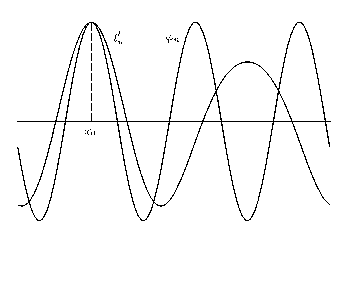
\includegraphics[width=0.5\textwidth]{pict/pict17-1.eps}
\end{center}
 \refstepcounter{ris}\label{r17-1}
 \centerline{Рис.~\theris}
\end{figure}

 \noindent
 Рассмотрим отрезок $\left[ x_0-\dfrac{\pi}{n}, x_0+\dfrac{\pi}{n}
 \right]=I,$ являющийся одним из наименьших периодов функции $\varphi_n.$
 Оказывается (см. рис.~\ref{r17-1}), что
$$
 \varphi_n(x)\le t_n'(x)\qquad \forall\ x\in
 \left[ x_0-\frac{\pi}{n}, x_0+\frac{\pi}{n}\right]=I.
$$
 Докажем это свойство рассуждениями  от противного. Предположим, что существует точка $x'\in I,$
 в которой $t_n'(x')< \varphi_n(x').$ {Тогда на промежутке $I$ кроме $x_0$ найдется}
{по крайней мере еще один нуль $x''$ функции
$t_n'-\varphi_n$ {(см. рис.~\ref{r17-2}).}}

\begin{figure}[ht]
\begin{center}
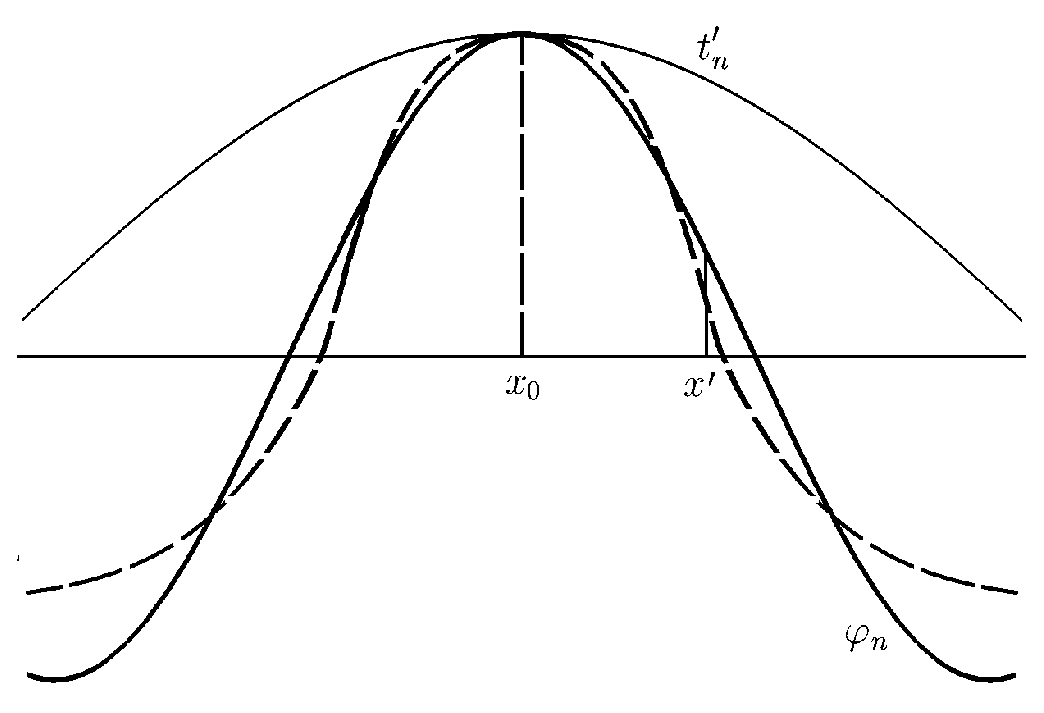
\includegraphics[width=0.5\textwidth]{pict/pict17-2.eps}
\end{center}
% \bigskip
 \refstepcounter{ris}\label{r17-2}

\centerline{Рис.~\theris}
\end{figure}

%\bigskip

% \noindent
 Будем считать нули разности $t_n'-\varphi_n.$  Рассмотрим отрезки, на которых
 $\cos n(x-x_0)$ один раз
 меняется от $-1$ до 1. На каждом из этих отрезков график $\varphi_n$
 пересекается с графиком  $t_n';$
 при этом, если пересечение осуществляется  в точке экстремума $\varphi_n$, то  эта
 точка является двойным корнем разности  $t_n'-\varphi_n.$ С учетом кратностей, график
 полинома $\varphi_n(x)=M_1 \cos n(x-x_0)$
 пересекает график  $t_n'$ {по крайней мере} столько раз, сколько $\cos n(x-x_0)$
 изменяется от $-1$ до 1. Таким образом, вне основного
 отрезка $I$ имеется $2n-2$ нуля разности $t_n'-\varphi_n,$
 {если она не зануляется в концах отрезка $I$;} кроме того,  на $I$
существуют еще два нуля -- в точке $x_0$ (двойной нуль) и в точке {$x''\in {\rm int}\, I$}
 (по предположению). Таким образом, при сделанном дополнительном предположении
 всего на периоде разность $t_n'-\varphi_n$ имеет
 (с учетом кратности), по крайней мере $2n-2+2+1=(2n+1)$
 нулей. {Ясно, что если $x''$ совпадает с одним из концов отрезка $I$ или
 функция $t_n'-\varphi_n$}
 {зануляется в обоих его концах, то общее число ее нулей на периоде
 не уменьшится.}  Однако  $t_n'-\varphi_n$ есть (ненулевой)  тригонометрический
 полином порядка $n$
 и не может иметь столько нулей  (на периоде). Пришли к противоречию. Значит,
 действительно, справедливо неравенство
 $$
 M_1\cos n(x-x_0)\le t_n'(x)\qquad \forall\ x\in
 \left[ x_0-\frac{\pi}{n},x_0+\frac{\pi}{n} \right].
 $$

 Проинтегрируем последнее неравенство по $x$ на
 $ \left[ x_0-\dfrac{h}{2},x_0+\dfrac{h}{2} \right]\subset I$
 при $0<h<\dfrac{2\pi}{n}.$ В результате получим
 $$
 M_1 \int_{x_0-\frac{h}{2}}^{x_0+\frac{h}{2}}\cos n(x-x_0)\, dx=
 \frac{M_1}{n} 2\sin \frac{nh}{2}\le
 $$
 $$
 \le \int_{x_0-\frac{h}{2}}^{x_0+\frac{h}{2}} t_n'(x)\, dx=
 t_n\left(x_0+\frac{h}{2}\right)- t_n\left(x_0-\frac{h}{2}\right)\le
 \|\Delta_ht_n\|_C
 $$
 и, так как $M_1=\|t_n'\|_C,$ то лемма при $k=1$ доказана.
 Пусть при $0<h<\dfrac{2\pi}{n}$ верно неравенство
 $$
 \|t_n^{(k-1)}\|\le \bigg( \dfrac{n}{2\sin\frac{nh}{2}}\bigg)^{k-1}\|\Delta_h^{k-1}
 t_n\|_C.
 $$
 Тогда при $0<h'<\dfrac{2\pi}{n}$ по доказанному
 неравенству
 $$\|t_n^{(k)}\|_C\le \dfrac{n}{2\sin\frac{nh'}{2}}\|\Delta_{h'} t_n^{(k-1)}\|_C=
\bigg(
\dfrac{n}{2\sin\frac{nh'}{2}}\bigg)\|(\Delta_{h'}
t_n)^{(k-1)}\|_C\le
$$
$$
\le \bigg( \dfrac{n}{2\sin\frac{nh'}{2}}\bigg)
\left( \dfrac{n}{2\sin nh}\right)^{k-1}\|\Delta_h^{k-1}(\Delta_{h'} t_n)\|.
$$
Полагая теперь $h'=h\in \Big(0,\dfrac{2\pi}{n}\Big),$
получим требуемое

%\newpage
 Д\;о\;к\;а\;з\;а\;т\;е\;л\;ь\;с\;т\;в\;о\quad теоремы~\ref{t17-1}.
 Представим разность $f-t_n$ в виде
 $$
 f-t_n=f-\sigma_{n+p,p}(f)-(t_n-\sigma_{n+p,p}(f)).
 $$
 Продифференцируем это тождество $k$ раз:
 $$
 f^{(k)}-t_n^{(k)}=f^{(k)}-\sigma_{n+p,p}(f^{(k)})-(t_n-
 \sigma_{n+p,p}(f))^{(k)}.
 $$
Отсюда получаем
 $$
 \|f^{(k)}-t_n^{(k)}\|_C\le \|f^{(k)}-\sigma_{n+p,p}(f^{(k)})\|_C+\|(t_n-
 \sigma_{n+p,p}(f))^{(k)}\|_C.
 $$
 Применяя неравенство Лебега  (для метода Валле Пуссена), имеем
 $$
 \|f^{(k)}-\sigma_{n+p,p}(f^{(k)})\|_C\le
 ({\|\sigma_{n+p,p}\|_C^C}+1) E_n(f^{(k)})_C.
 $$
 Далее, применяя неравенство Бернштейна и вновь неравенство  Лебега, получаем
 $$
 \|(t_n-
 \sigma_{n+p,p}(f))^{(k)}\|_C\le (n+p)^k \|t_n-
 \sigma_{n+p,p}(f)\|_C\le
 $$
 $$
 \le
  (n+p)^k (\|f-t_n\|_C+\|f-
 \sigma_{n+p,p}(f)\|_C)
 \le
 $$
 $$
 \le (n+p)^k \left\{
 \|f-t_n\|_C+({\|\sigma_{n+p,p}\|_C^C}+1)\|f-t_n\|_C\right\} =
 $$
 $$
 =({\|\sigma_{n+p,p}\|_C^C}+2)  (n+p)^k
 \|f-t_n\|_C.
 $$
 Таким образом,  справедливо неравенство
 \begin{equation}\label{f17-1}
 \|f^{(k)}-t_n^{(k)}\|_C\le (\|\sigma_{n+p,p}\|_C+2) \left\{ (n+p)^k
 \|f-t_n\|_C+E_n(f^{(k)})_C\right\}. %\eqno(1)
 \end{equation}

 Положим здесь $p=n.$ По  теореме Никольского нормы $\|\sigma_{2n,n}\|$
 ограничены (по $n$). Поэтому  из {\eqref{f17-1}} следует оценка
 $$
 \|f^{(k)}-t_n^{(k)}\|_C\le A_k \left\{ n^k \|f-t_n\|_C+E_n
 (f^{(k)})_{{C}}\right\}.
 $$
 Теорема доказана.

 \begin{Remark} %%%Замечание.
 Приведенное  доказательство дает значение $A_k=O(2^k).$ На самом деле можно получить   $A_k=O(\ln(k+1)).$
 Для обоснования этого необходимо   надлежащим образом выбрать
 параметр $p.$ Из оценки {\eqref{f17-1}}  по теореме
 Никольского получим
 $$
 \|f^{(k)}-t_n^{(k)}\|_C\le \left\{ \frac{4}{\pi^2}\ln
 \frac{n+p}{p+1}+O(1) \right\} \left( \frac{n+p}{n}\right)^k \left(
 n^k \|f-t_n\|_C+E_n (f^{(k)})_C\right).
 $$
 Путем выбора $p=p(n)$ сделаем величину
  \begin{equation}\label{f17-2}
\left\{ \frac{4}{\pi^2}\ln \frac{n+p}{p+1}+O(1)\right\} \left(
 \frac{n+p}{n}\right)^k %\eqno(2)
  \end{equation}
 как можно меньше. Рассмотрим два случая.

 {\Case $k\le n.$} Выберем целое $p$ так, чтобы $\dfrac{n}{k}-1\le p\le \dfrac{n}{k}.$
 Тогда
 $$
 \left( \frac{n+p}{n}\right)^k \le \left( 1+
 \frac{{n}/{k}}{n}\right)^k = \left(
 1+\frac{1}{k}\right)^k\le e,
 $$
 $$
 \frac{n+p}{p+1}=\frac{n-1}{p+1}+1\le k\frac{n-1}{n}+1< k+1.
 $$
 При таком выборе параметра $p$ величина {$\eqref{f17-2}$}
 будет иметь значение   $O(\ln(k+1)),$ т.\,е. $A_k=O(\ln(k+1)).$

 {\Case $k\ge n.$}
 \noindent  Положим $p=0.$ В этом случае для величины {$\eqref{f17-2}$}  имеем {оценку}
 $$
 \frac{4}{\pi^2} \ln (n+1)+O(1)\le
 \frac{4}{\pi^2} \ln (k+1)+O(1)=O(\ln(k+1)).
 $$
 Итак, в обоих случаях получаем
 $$
 A_k=O(\ln(k+1)).
 $$
 \end{Remark}

 \task %%% Задача.
 Доказать, что этот порядок величины $A_k$ является точным.

 \begin{Remark} %%%Замечание.
 Неравенство Бернштейна~(\ref{17-2}) доказано нами в пространстве $C_{2\pi}.$
 Однако, как можно показать, оно имеет место и в любом однородном пространстве. Поэтому и
 теорема~\ref{t17-1} о дифференцировании приближающих полиномов
 верна не только в $C,$ но и в любом однородном пространстве (см. замечание в конце п.~17.1).
 \end{Remark}

 % Лекции Сергея Борисовича Стечкина
% Внесены исправления В.В.Арестова, версия 06.07.2009
% Внесены исправления Н.И.Черныха, версия 24.07.2009
% Внесена грамматическая и ТеХ-правка М.Дейкаловой, версия 05.08.09

 %%%%%%%%%%%%%%%%%%%%%%%%%%%%%
 \chapter{Приближение истокообразно представимых функций}
  %%{Лекция 18.}



 \section{Приближение  функций в пространстве  $L_{2\pi}$
 %\\ тригонометрическими полиномами
 }

Рассмотрим вначале  наилучшее приближение функций в пространстве $L= L_{2\pi},$
наделенном нормой
$$
\|f\|_L=\frac{1}{\pi}\int_{0}^{{2\pi}}|f(t)|dt,
$$ тригонометрическими
 полиномами
 $$
 t_{n-1}(x)=\frac{\alpha_0}{2}+\sum\limits_{k=1}^{n-1} (\alpha_k\cos
 kx+\beta_k \sin kx)
 $$
 порядка $n-1,$~ $n\ge 1.$



 \begin{teo}\label{approx_L} \it{ Для функций  $f\in L_{2\pi}$ справедливы
 следующие два утверждения:

 $1)$ Если для тригонометрического полинома $t_{n-1}^{{*}}$ функция, равная знаку разности
 $R=f-t_{n-1}^{{*}},$ ортогональна пространству ${\cal T}_{n-1}:$
 \begin{equation}\label{f18-1}
 \sign R \perp {t_{n-1}}\qquad \forall\  {t_{n-1}\in\mathcal{T}_{n-1}}, %\eqno(1)
  \end{equation}
 то $t_{n-1}^*$  --  полином наилучшего приближения функции $f$ в $L_{2\pi}$.


 $2)$ Если  $t_{n-1}^{{*}}$ -- полином наилучшего приближения функции $f$ и разность
 $f-t_{n-1}^{{*}}$ почти всюду отлична от нуля, то обязательно выполняется
 условие~$(\ref{f18-1}).$}
 \end{teo}

 В конце лекции 9 говорилось о возможном выводе подобного
 результата для приближения в $L(Q)$ из приведенного там
 доказательства критерия элемента наилучшего приближения в
 $L^p(Q).$ Ниже приводится полное доказательство для
 рассматриваемого частного случая.


 \begin{proof}
 %Д о к а з а  т е л ь с т в о\ \  л е м м ы.
 Предположим, что для
 тригонометрического полинома $t_{n-1}^{{*}}$ выполняется свойство~$(\ref{f18-1}),$
 т.\,е.  функция $\sign R$
 ортогональна  любому полиному порядка $n-1.$ Тогда  для любого полинома
 {$t_{n-1}\in {\cal T}_{n-1}$}
 $$
 \|f-t_{n-1}^{{*}}\|_L=\frac{1}{\pi}\int_0^{2\pi} |f(x)-t_{n-1}^{{*}}(x)|\, dx=
 \frac{1}{\pi}\int_0^{2\pi} (f(x)-t_{n-1}^{{*}}(x))\ \sign R(x)\, dx=
 $$
 $$
 =\frac{1}{\pi}\int_0^{2\pi} ((f(x)-{t}_{n-1}(x))+({t}_{n-1}(x)-t_{n-1}^{{*}}(x)))\
 \sign R(x)\, dx=
 $$
 $$
 =\frac{1}{\pi}\int_0^{2\pi} (f(x)-{t}_{n-1}(x))\ \sign R(x)\, dx\le
 \frac{1}{\pi}\int_0^{2\pi} |f(x)-{t}_{n-1}(x)|\, dx=\|f-{t}_{n-1}\|_L.
 $$
Следовательно, $t_{n-1}^{{*}}$ -- наилучший полином для функции $f$ в {$L_{2\pi}$
среди полиномов из $\mathcal{T}_{n-1}$.}

Предположим теперь, что $t_{n-1}^{{*}}$ -- полином наилучшего
приближения функции $f$ и почти всюду $t_{n-1}^{{*}}\ne f.$ Для произвольного полинома
${t}_{n-1}$ порядка $n-1$ определим функцию
$$
\Phi(\lambda)=\|f-(t_{n-1}^{{*}}-\lambda {t}_{n-1})\|_L=\frac{1}{\pi}\int_{0}^{2\pi}|f(x)
-t_{n-1}^{{*}}(x)+\lambda {t}_{n-1}(x))|\, dx
$$
вещественного переменного $\lambda.$
Убедимся, что функция $\Phi$ дифференцируема в точке $\lambda=0$ и
вычислим производную $\Phi'(0).$

Для вещественных чисел $a\ne 0$ и $b$ функция $\phi(\lambda)=|a+\lambda b|$ переменного
$\lambda$  дифференцируема в точке $\lambda=0$ и $\phi'(0)=b\ \sign a.$ Кроме того,
имеет место неравенство
$$
\left|\frac{|a+\lambda b|-|a|}{\lambda}\right|\le |b|,\qquad \lambda\ne 0.
$$
Применяя теорему Лебега о мажорантной сходимости, теперь нетрудно убедиться, что функция
$\Phi$ дифференцируема  в точке $\lambda=0$ и
$$
\Phi'(0)=\frac{1}{\pi}\int_{0}^{2\pi}\  {t}_{n-1}(x)\ \sign (f(x)-t_{n-1}^{{*}}(x))\,dx.
$$
В силу экстремальности полинома $t_{n-1}^{{*}}$ точка $\lambda=0$ является точкой минимума
функции~$\Phi;$ поэтому  $\Phi'(0)=0$ и мы пришли к свойству~$(\ref{f18-1}).$
Теорема~\ref{f18-1} доказана.
\end{proof}

 Заметим, что если выполняется условие~(\ref{f18-1}), то
 $$
 E_{n-1}(f)_L=\frac{1}{\pi}\int_0^{2\pi} (f(x)-t_{n-1}^{{*}}(x))\ \sign R(x)\, dx=
 \frac{1}{\pi}\int_0^{2\pi} f(x)\ \sign R(x)\, dx
 $$
и, окончательно,
 \begin{equation}\label{f18-2}
 E_{n-1}(f)_L=\frac{1}{\pi}\int_0^{2\pi} f (x)h^*(x)\, dx,%\eqno(2)
 \end{equation}
где $h^*=\sign R;$ при этом функция $h^*$ обладает свойствами
$\|h^*\|_{{L^\infty}}\le 1$ и $h^*\perp {t}_{n-1}$ для любого полинома
$t_{n-1}.$



 \begin{teo} %%% Теорема.
 Пусть $f\in L_{2\pi}.$ Тогда для любой функции {$h\in L_{2\pi}^\infty$} со свойствами
 $$
 \|h\|_{{L^\infty}}\le 1\quad \textit{и}\quad h\perp
 {t}_{n-1}\qquad \forall\ {t}_{n-1}
 $$
 выполняется неравенство
  \begin{equation}\label{f18-3}
 E_{n-1}(f)_L\ge \frac{1}{\pi}\int_0^{2\pi} f(x) h(x)\, dx.%\eqno(3)
  \end{equation}
 \end{teo}

 \begin{proof} %%% Доказательство.
 Пусть $t_{n-1}^*$ -- полином наилучшего приближения функции $f$ в $L.$
 В силу ортогональности функции  $h$ полиномам порядка $n-1$
 $$
 \frac{1}{\pi}\int_0^{2\pi} f(x)h(x)\, dx=\frac{1}{\pi}\int_0^{2\pi} (f(x)-t_{n-1}^*(x))h(x)\,dx\le
 \frac{1}{\pi}\int_0^{2\pi} |f(x)-t_{n-1}^*(x)|\,dx=E_{n-1}(f)_L.
 $$
  Теорема доказана.
 \end{proof}

\setcounter{corollary}{0}
\begin{corollary}
Предположим, что  $t_{n-1}^*$ -- полином наилучшего в $L_{2\pi}$
приближения  для функции $f$ и
функция  $h^*=\sign (f-t_{n-1}^*)$ удовлетворяет  условию~$(\ref{f18-1})$ $($к примеру,
разность $f-t_{n-1}^*$ не равна нулю почти всюду$).$ Тогда
 $$
 E_{n-1}(f)_L=\frac{1}{\pi}\int_0^{2\pi} f(x)h^*(x)\,dx=
 $$
 $$=\max \left\{\frac{1}{\pi}\int_0^{2\pi} f(x)h(x)\,dx:\
 h\in {L_{2\pi}^\infty},\ \|h\|_{{L^\infty}}\le 1;\ h\perp {t_{n-1}}\
 \forall\ {t_{n-1}}\in {\cal T}_{n-1}\right\}.
 $$
\end{corollary}

\begin{corollary}  Если полином {$t_{n-1}^*$} таков, что  разность {$f-t_{n-1}^*$} почти всюду
отлична от нуля и функция $h^{{*}}=\sign (f-t_{n-1}^{{*}}) $ ортогональна
пространству полиномов порядка $n-1,$ то {$t_{n-1}^*$} --
полином наилучшего приближения в $L_{2\pi}$ для функции $f,$ и неравенство
{\eqref{f18-3}} на функции $h^{{*}}$ и только на этой функции обращается в
равенство.
\end{corollary}

\ \

Любая функция $h$ {из $L_{2\pi}^\infty$} со свойствами
$$
\|h\|_{{L^\infty}}\le 1\quad \text{и}\quad h\perp t_{n-1}\qquad \forall\
t_{n-1}\in {\cal T}_{n-1}
$$
дает в силу {\eqref{f18-3}} для величины $E_{n-1}(f)_L$ оценку снизу.
 Выберем специальным образом функцию  $h.$ Предположим, что  $h$ имеет период  $\omega=\dfrac{2\pi}{n}$
 и $\ds\int_{-\pi}^{\pi} h(x)\, dx=0.$ Тогда ряд Фурье такой функции имеет вид
  $$
 h(x) \sim \sum\limits_{k=1}^{\infty} \alpha_{nk}\cos nkx+\beta_{nk}\sin nkx,
 $$
 т.\,е. у функции $h$ могут быть  отличны от нуля только коэффициенты
 Фурье, номера которых кратны числу $n.$
 В частности, выполняется свойство
 $$
 h\perp {t}_{n-1}\qquad \forall\  {t}_{n-1}.
 $$
 Поэтому в качестве $h$ в {\eqref{f18-3}}
 можно взять любую такую функцию (удовлетворяющую, помимо того, условию
 {$\|h\|_{L^\infty}\le 1$}).


 Возьмем функцию $h(x)=\sign \sin(nx+\alpha).$ Эта функция обладает
 всеми перечисленными свойствами: ее период
  $\omega$ равен $\dfrac{2\pi}{n},$~
 $ \dfrac{1}{\pi}\displaystyle\int_{-\pi}^{\pi} h(x)\, dx=0$ и {$\|h\|_{L^\infty}\le 1.$}
 Поэтому
  \begin{equation}\label{f18-4}
 E_{n-1}(f)_L\ge \frac{1}{\pi}\int_{-\pi}^{\pi} f(x)\, \sign\sin(nx+\alpha)\, dx\qquad
 \forall\ \alpha.%\eqno(4)
  \end{equation}
 Рассмотрим случаи $\alpha=0$ и $\alpha=\dfrac{\pi}{2}.$ Хорошо известно разложение
 $$
 \sign \sin x=\frac{4}{\pi}\sum\limits_{k=0}^{\infty}\frac{\sin
 (2k+1)x}{2k+1}.
 $$
Следовательно,
 %\addtocounter{equation}{1}
 \refstepcounter{equation}\label{f18-5}
 $$
 \sign \sin nx=\frac{4}{\pi}\sum\limits_{k=0}^{\infty}\frac{\sin
 (2k+1)nx}{2k+1}.\eqno(\theequation')
 $$
 Аналогично,
 $$
 \sign \cos x=\sign \sin\left( x+\frac{\pi}{2}\right)
 =\frac{4}{\pi}\sum\limits_{k=0}^{\infty}\frac{(-1)^k\cos
 (2k+1)x}{2k+1},
 $$
 $$
 \sign \cos nx=\frac{4}{\pi}\sum\limits_{k=0}^{\infty}
 \frac{(-1)^k\cos (2k+1)nx}{2k+1}.\eqno(\theequation'')
 $$
 В силу {\eqref{f18-4}}  для любой функции $f\in L$ справедливы
 $\Big($получаемые соответственно, при $\alpha=0$ и $\alpha=\dfrac{\pi}{2}\Big)$ оценки
 \begin{equation}\label{f18-6}
 E_{n-1}(f)_L\ge \frac{4}{\pi}\sum\limits_{k=0}^{\infty}
 \frac{b_{(2k+1)n}}{2k+1}, %\eqno(6)
 \end{equation}
 \begin{equation}\label{f18-7}
 E_{n-1}(f)_L\ge \frac{4}{\pi}\sum\limits_{k=0}^{\infty}
 \frac{(-1)^k a_{(2k+1)n}}{2k+1}, %\eqno(7)
 \end{equation}
 где $a_{(2k+1)n}$ и $b_{(2k+1)n}$ -- соответствующие индексам коэффициенты Фурье
  функции $f.$
    Заметим, что если $\alpha=\pi,$
 то $h(x)=-\sign \sin nx,$ если $\alpha=\dfrac{3}{2}\,\pi,$
 то $h(x)=-\sign\cos nx,$ и получим аналогичные оценки
 $$
 E_{n-1}(f)_{L}\ge
 -\frac{4}{\pi}\sum\limits_{k=0}^{\infty}\frac{b_{(2k+1)n}}{2k+1},
 \eqno(\ref{f18-6}')
 $$
 $$
 E_{n-1}(f)_{L}\ge
 -\frac{4}{\pi}\sum\limits_{k=0}^{\infty}\frac{(-1)^k a_{(2k+1)n}}{2k+1}.
 \eqno(\ref{f18-7}')
 $$

 Возникает вопрос, когда последние четыре оценки обращаются в равенство?
 Пусть $t_{n-1}^*$ -- полином наилучшего приближения функции $f.$
 Будем исходить из того, что   почти для всех  точек $x\in(-\pi,\pi)$ выполняется свойство $f(x)-t_{n-1}^*(x)\ne 0.$
 Равенство в {\eqref{f18-6}} возможно только в том случае, когда (почти всюду)
 \begin{equation}\label{f18-8}
 \sign(f-t_{n-1}^*)=\sign\sin nx; %\eqno(8)
 \end{equation}
 равенство в {\eqref{f18-7}} может быть, только если
 \begin{equation}\label{f18-9}
 \sign(f-t_{n-1}^*)=\sign\cos nx. %\eqno(9)
 \end{equation}
 Аналогично, равенство в~{$(\ref{f18-6}')$ и~$(\ref{f18-7}')$} будет, когда, соответственно,
 $$
 \sign(f-t_{n-1}^*)=-\sign\sin nx, \eqno(\ref{f18-8}')
 $$
 $$
 \sign(f-t_{n-1}^*)=-\sign\cos nx. \eqno(\ref{f18-9}')
 $$


 Предположим, что функция $f$ непрерывна на интервале $(-\pi,\pi).$
 Тогда {\eqref{f18-9} и~$(\ref{f18-9}')$} означают, что разность
 $f-t_{n-1}^*$ меняет знак в тех и только тех точках, где $\cos nx$
 обращается в нуль, и, значит, $t_{n-1}^*$ интерполирует $f$
 в нулях $\cos nx;$ аналогично,~{\eqref{f18-8} и~$(\ref{f18-8}')$}
 влекут, что $t_{n-1}^*$ интерполирует $f$ в нулях $\sin nx.$
 Эти условия интерполяции -- необходимые условия справедливости
 (для непрерывной функции) равенств в~{\eqref{f18-7}, $(\ref{f18-7}')$,
 \eqref{f18-6}, $(\ref{f18-6}')$,}
 соответственно. Однако в некоторых ситуациях они являются и  достаточными.
  Действительно, если полином $t_{n-1}$ интерполирует функцию $f,$ к примеру, {только}
 в нулях $\cos nx$ и разность $f-t_{n-1}$
 меняет знак в этих нулях и нигде больше, то в~{\eqref{f18-7}
  или~$(\ref{f18-7}')$}, соответственно,
 имеет место равенство и {$t_{n-1}^*$}
 является наилучшим полиномом для $f$ {в $L_{2\pi}$.} {В этих ситуациях}
 $$
 E_{n-1}(f)_L=\frac{4}{\pi}\left|\sum\limits_{k=0}^{\infty}
 \frac{b_{(2k+1)n}}{2k+1}\right|, \eqno(\ref{f18-6}'')
 $$
  $$
 E_{n-1}(f)_L=\frac{4}{\pi}\left|\sum\limits_{k=0}^{\infty}
 \frac{(-1)^k a_{(2k+1)n}}{2k+1}\right|.\eqno(\ref{f18-7}'')
 $$

 Таким образом, мы получили способ нахождения
 наилучшего полинома в $L_{2\pi}$ для $f\in C_{2\pi}$:
 выбираем $h(x)=\sign \sin nx,$ если $f$ -- нечетная, $h(x)=\sign \cos nx,$
 если $f$ -- четная (для других случаев следует рассмотреть функцию
 $\sign \sin (nx+\alpha)$ и попытаться подобрать соответствующим образом значение параметра
 $\alpha$). Затем строим полином, который
 интерполирует $f$ в нулях, соответственно, $\sin nx$ или $\cos nx$
 и проверяем знаки разности. Если они удовлетворяют
 соответствующим условиям~{\eqref{f18-8}, $(\ref{f18-8}'),$ \eqref{f18-9} или~$(\ref{f18-9}')$,}
 то наилучший полином построен. Так что задача построения
 наилучшего полинома в $L_{2\pi}$
 сводится к проверке знака разности $f-t_{n-1}^*.$
 Если знаки не проверять, то~{\eqref{f18-7}, $(\ref{f18-7}')$ и~\eqref{f18-6}
 или~$(\ref{f18-6}')$}
 дают оценку для $E_{n-1}(f)_L$ снизу.


 \section{Приближение классов функций в ${C}_{2\pi}$}

 Пусть  $K\in L_{2\pi};$ функцию $K$ будем называть  суммируемым  ядром.
 Рассмотрим класс функций $\G M=\G M_K,$  истокообразно представимых при помощи
 этого ядра, т.\,е. класс  функций вида
 \begin{equation}\label{f18-10}
 f(x)=c+\frac{1}{\pi}\int_0^{2\pi} K(t)\varphi(x+t)\,dt, %\eqno(10)
 \end{equation}
 где  $\varphi$ -- произвольная $2\pi$-периодическая функция из пространства
 {$L^\infty=L_{2\pi}^{\infty}$}
 со свойством $\|\varphi\|_{{L^\infty}}\le 1,$ а $c=c(f)$ -- вещественная константа.
 Функции из класса $\G M$ будут непрерывными $2\pi$-периодическими. Каждую
  функцию $f\in \G M$
  наилучшим образом приблизим тригонометрическими
 полиномами в $C_{2\pi}$ и возьмем
 $$
 \sup_{f\in \G M} \min_{t_{n-1}}\|f-t_{n-1}\|_C=E_{n-1}(\G M_K)_C;
 $$
 эту величину называют наилучшим приближением класса $\G M$
 в пространстве $C_{2\pi}$ множеством
 тригонометрических полиномов порядка $n-1$.

 Для любого тригонометрического полинома {$\widetilde{t}_{n-1}$}  функция
 $$
 t_{n-1}(x)=c+ \frac{1}{\pi}\int_0^{2\pi} \-{\widetilde{t}_{n-1}(t)} \varphi(x+t)\, dt
 $$
также является тригонометрическим полиномом  порядка $n-1$, и для него при
$c=c(f)$ имеем
 $$
 |f(x)-t_{n-1}(x)|=\left| \frac{1}{\pi}\int_0^{2\pi} \{ K(t)-{\widetilde{t}_{n-1}(t)}\}
 \varphi(x+t)\, dt \right|\le \frac{1}{\pi}\int_0^{2\pi} | K(t)-{\widetilde{t}_{n-1}(t)}|\, dt,
 $$
а, значит,
 $$
 \|f-t_{n-1}\|_C\le \frac{1}{\pi}\int_0^{2\pi} |K-{\widetilde{t}_{n-1}}|\,
 dt \qquad \forall \ {\widetilde{t}_{n-1}}.
 $$
 Отсюда заключаем, что
 $$
 E_{n-1}(f)_C\le E_{n-1}(K)_L\qquad \forall \ f\in \G M_K.
 $$
 Следовательно, имеет место неравенство
 \begin{equation}\label{f18-11}
 \sup_{f\in \G M_K} E_{n-1}(f)_C \le E_{n-1}(K)_L. %\eqno(11)
 \end{equation}
{Можно указать широкий класс ядер $K,$ когда на самом деле здесь имеет место равенство;
ниже это будет сделано для важного конкретного случая.}

 Приведенные выше рассуждения можно повторить в любом однородном
 пространстве $H$ $2\pi$-периодических функций, норма в котором инвариантна относительно сдвига.
 Вновь будем  иметь
 $$
 \|f-t_{n-1}\|_H=\left\| \frac{1}{\pi}\int_0^{2\pi}\{K(t)-{\widetilde{t}_{n-1}(t)}\}
 \varphi(x+t)\, dt\right\|_H\le
 $$
 $$
 \le \frac{1}{\pi}\int_0^{2\pi} |K(t)-{\widetilde{t}_{n-1}(t)}|\ \|\varphi(\cdot +t)\|_H\, dt=
 \frac{1}{\pi}\int_0^{2\pi} |K(t)-{\widetilde{t}_{n-1}(t)}|\, dt \cdot \|\varphi\|_H
 $$
 и, следовательно,
 $$
 E_{n-1}(f)_H \le E_{n-1}(K)_L\cdot \|\varphi\|_H.
 $$
 Обозначим через  $\G M_{K,H}$ класс функций в $H$ вида {\eqref{f18-10}},
 у  которых $\varphi\in H,$~ $\|\varphi\|_H\le 1.$ Тогда получим
 $$
 \sup_{f\in \G M_{K,H}} E_{n-1}(f)_H\le E_{n-1}(K)_L.
 $$
 В общем случае здесь равенства не будет.

 \section{Приближение ядра Бернулли\\ тригонометрическими полиномами в среднем}



 Теперь рассмотрим класс ${W_1^{(r)}},$~ $r\ge 1,$ функций $f\in C_{2\pi},$
 у которых производная $f^{(r-1)}$
 порядка $r-1$ принадлежит классу ${\rm Lip\ }1$ с константой $1,$
 т.\,е. удовлетворяет условию
 $$
 |f^{(r-1)}(x')-f^{(r-1)}(x'')|\le |x'-x''|\qquad \forall\ x',x''.
 $$
 У функции $f\in {W_1^{(r)}}$ почти всюду  существует производная  $f^{(r)}$ порядка $r,$
  при этом $|f^{(r)}(x)|\le 1$ почти всюду и
 $$\frac{1}{\pi}\int_0^{2\pi}f^{(r)}(x)\, dx=0,$$
 т.\,е. производная $f^{(r)}$
 имеет нулевое среднее значение на периоде. Функция $f\in {W_1^{(r)}}$  допускает следующее интегральное
 представление:
 \begin{equation}\label{f18-12}
 f(x)=\frac{a_0}{2}+\frac{1}{\pi}\int_{-\pi}^{\pi} K_r(t) f^{(r)}(x+t)\, dt, %\eqno(12)
 \end{equation}
 где $\dfrac{a_0}{2}=\dfrac{1}{2\pi}\displaystyle\int_0^{2\pi}f(x)\,dx$
 -- среднее значение функции $f,$ а
 \begin{equation}\label{f18-13}
 K_r(t)=\sum\limits_{n=1}^{\infty}\frac{\cos\left( nt+\frac{r\pi}{2}\right)} {n^r}. %\eqno(13)
 \end{equation}
 Функцию $K_r$ называют ядром Бернулли.

 При $r=1$ имеем
 $$
 K_1(t)=-\sum\limits_{n=1}^{\infty}\frac{\sin nt}{n}=\frac{t-\pi}{2},\qquad
 t\in (0,2\pi).
 $$
 При $r>1$ ядро  $K_r$  получается интегрированием ядра  $K_{r-1}$ с условием выбора константы интегрирования так, чтобы среднее значение было равно нулю:
 $$
\frac{1}{2\pi} \int_0^{2\pi} K_r(t)dt=0.
 $$




 В силу результатов предыдущего параграфа для функций $f\in {W_1^{(r)}}$ справедливо неравенство
 $$
 E_{n-1}(f)_C\le E_{n-1}(K_r)_L.
 $$
 Вычислим величину $E_{n-1}(K_r)_L.$ Вместо $K_r$ нам удобно вычислить наилучшее приближение функции
 $$
 K_r(t+\pi)=\sum\limits_{n=1}^{\infty}(-1)^n\frac{\cos\left( nt+\frac{r\pi}{2}\right)} {n^r},
 $$
 эту функцию вновь обозначим символом $K_r.$ В силу свойства $2\pi$-периодичности
 величина наилучшего приближения при этом не изменится. В новых обозначениях имеем
 $$
 K_1(t)=\frac{t}{2},\qquad t\in (-\pi,\pi).
 $$
Функция $K_r$ является нечетной или четной в соответствии с тем, будет ли число $r$ нечетным или четным.

Построим для ядер  $K_r$
 интерполяционные полиномы $U_{n-1}$ с узлами в нулях $\sin nx$, если число $r$ нечетное,
 и в нулях  $\cos nx$, если число $r$ четное.
 Ближайшая наша задача состоит в том, чтобы доказать, что разность  $R=K_r-U_{n-1}$
 меняет знак лишь в точках интерполирования.
 В случае $r=1$ функция $K_1$ (см. рис.~\ref{r18-1}) имеет разрывы в точках $(2k+1)\pi;$ эти точки следует
 считать точками перемены знака разности $R.$
 В случае  $r=2s+1,$~ $s>0,$  точки $\pm\pi$ оказываются еще и дополнительными узлами
 интерполирования.

\begin{figure}[ht]
\begin{center}
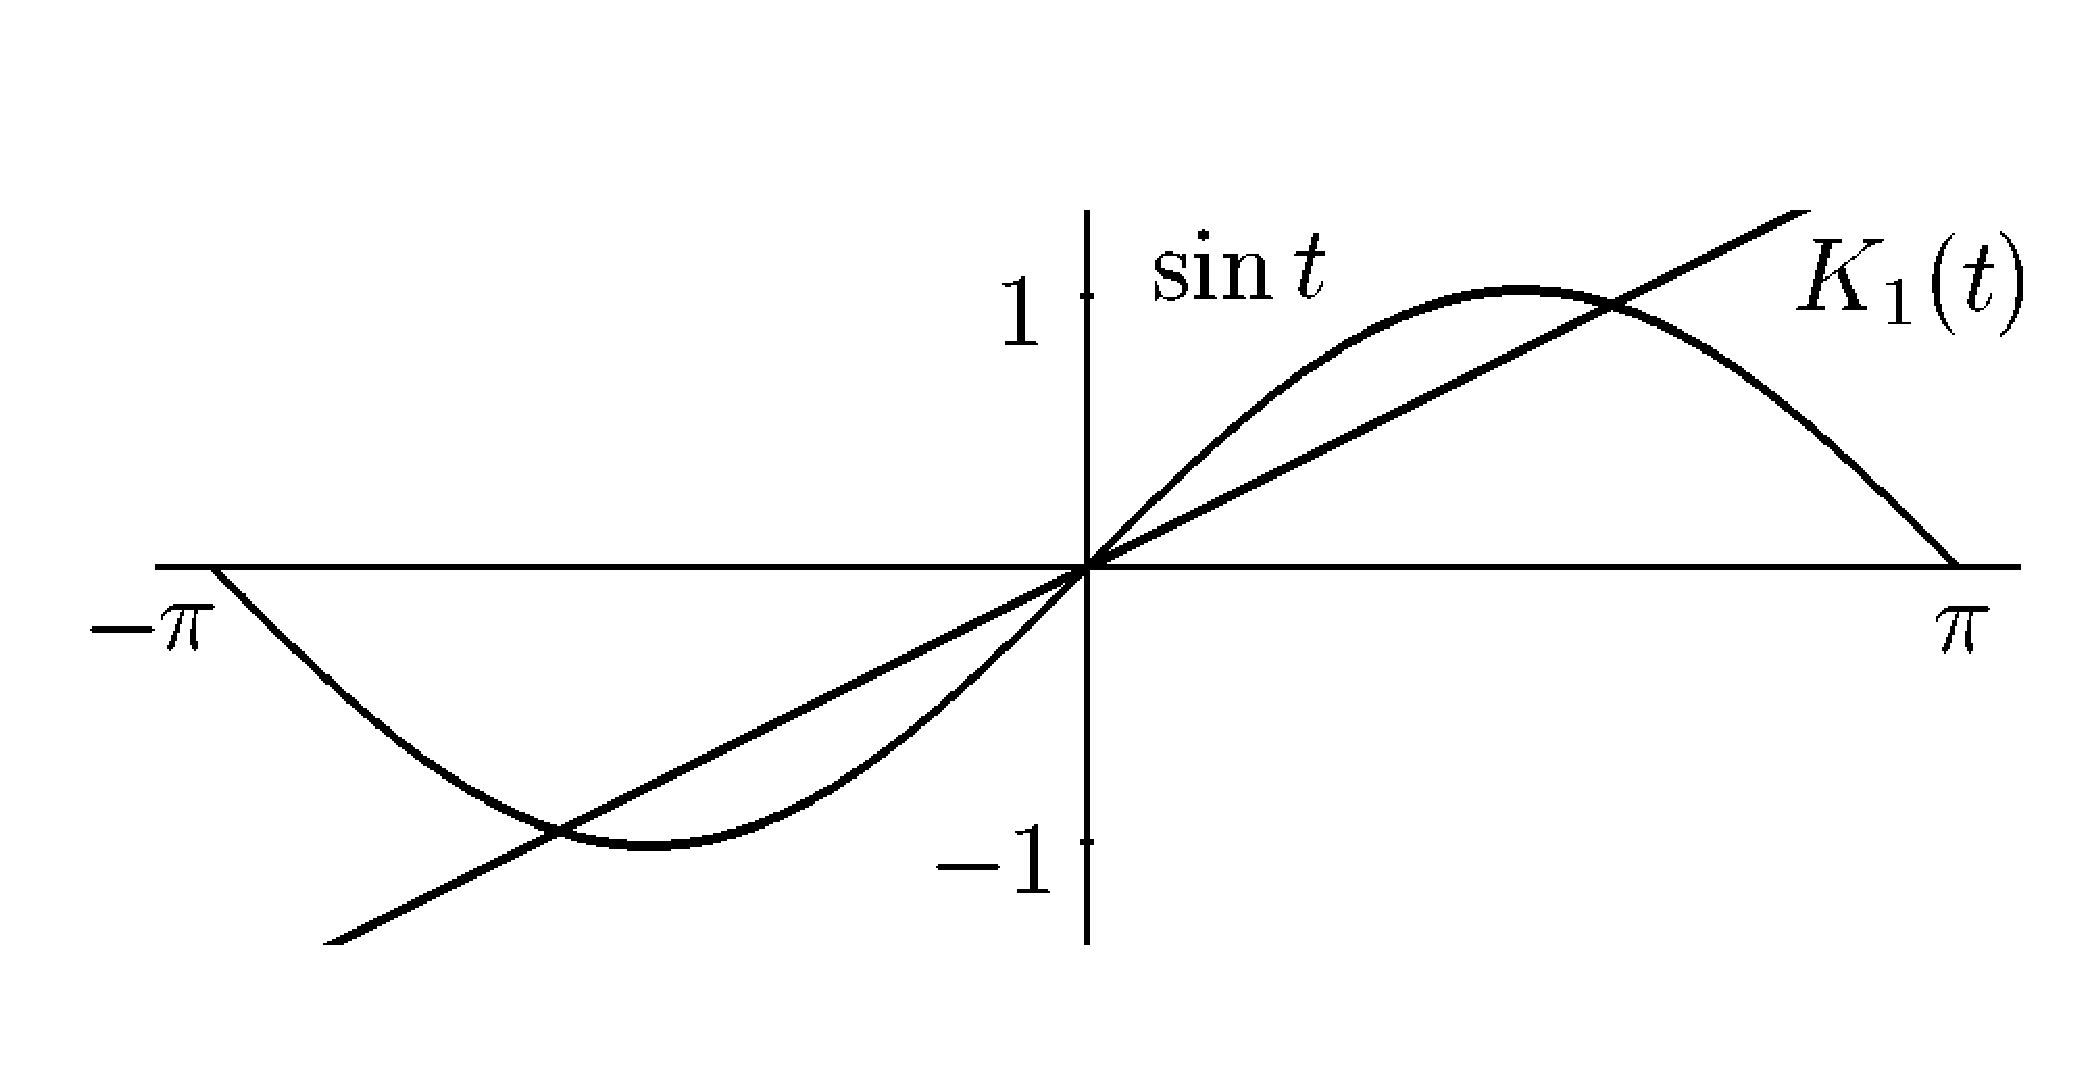
\includegraphics[width=0.5\textwidth]{pict/pict18-1.eps}
\end{center}
 \refstepcounter{ris}\label{r18-1}

 \centerline{Рис.~\theris}
\end{figure}





 \begin{lemma}\label{l18-2}
 Разность $R=K_r-U_{n-1}$ ядра $K_r$ и интерполяционного
 полинома
 $U_{n-1}$ обладает свойством
 $$
 \sign(K_r(t)-U_{n-1}(t))=\pm \sign \sin nt,\qquad t\in(-\pi,\pi),
 $$
  если число $r$ нечетное, и свойством
 $$
 \sign(K_r(t)-U_{n-1}(t))=\pm \sign \cos nt,\qquad t\in(-\pi,\pi),
 $$
  если число $r$ четное.
 \end{lemma}

Д\;о\;к\;а\;з\;а\;т\;е\;л\;ь\;с\;т\;в\;о\quad леммы~\ref{l18-2}.
Разность $R=K_r-U_{n-1}$ на $(-\pi,\pi)$ имеет $(2n-1)$ нулей при нечетном $r$ и
$2n$ нулей -- при четном $r.$ Для обоснования утверждений леммы достаточно
показать, что все эти нули простые и других нулей нет.

В свою очередь, для этого достаточно доказать, что при $r$ нечетном
для произвольного нечетного тригонометрического полинома $V_{n-1}$ порядка $n-1$ разность
$R=K_r-V_{n-1}$ имеет на $(-\pi,\pi)$ не более $(2n-1)$ нулей (с учетом их
кратности), а при четном $r$ и четном полиноме $V_{n-1}$
разность $R=K_r-V_{n-1}$  имеет на $(-\pi,\pi)$ не более
$2n$ нулей {(опять же с учетом их
кратности).} Докажем это утверждение  индукцией по $r\ge 1.$


1. Пусть $r=1.$ Покажем, что разность $R=K_1-V_{n-1}$ между ядром $K_1$ (оно в данном
случае нечетное) и нечетным тригонометрическим
  полиномом $V_{n-1}$ имеет на интервале $(-\pi,\pi)$ не более $(2n-1)$
  нулей (с учетом их кратности).
  Докажем этот факт от противного. Производная разности
 $$
 R'(t)=\frac{1}{2} -V_{n-1}'(t)=\frac{1}{2} -\sum\limits_{k=1}^{n-1}
 \alpha_k\cos kt,\qquad t\in (-\pi,\pi),
 $$
 есть (ненулевой) полином по  косинусам порядка $n-1$. Такой полином
 может иметь на $(-\pi,\pi)$
 не более $(2n-2)$ нулей. Если бы на $(-\pi,\pi)$ разность $R$ имела,
 по крайней мере,  $2n$
 нулей, то по теореме Ролля ее производная  $R'$ имела бы $(2n-1)$
 нулей, чего быть не может. Пришли к противоречию. Следовательно,
 $R=K_r-V_{n-1},$ действительно,
 имеет на $(-\pi,\pi)$ не более $(2n-1)$ нулей.

 2. Пусть $r=2.$ Ядро  $K_2$ и полином $V_{n-1}$  являются четными.
 Мы хотим  доказать, что разность
 $R=K_2-V_{n-1}$ имеет на $(-\pi,\pi)$
 не более $2n$ нулей.
 Имеем  $R'=K_2'(t)-V'_{n-1}$, где
 $V'_{n-1}$ есть  нечетный полином порядка $n-1$. Только что  мы уже доказали, что такая
 разность может иметь не более $(2n-1)$ нулей на $(-\pi,\pi).$
 Следовательно, $R$ может иметь не более $2n$ нулей.

 3. Докажем теперь, что если при  $r>1$ нужное свойство нулей  имеет место для номера $r-1,$ то оно имеет место и для номера $r.$    Пусть $r>1$ нечетное,
 $r=2s+1,$~ $s\ge 1.$
 Тогда $K_{2s+1}$ и $V_{n-1}$ нечетные и, следовательно  $K_{2s+1}$
 и $V_{n-1}$ обращаются в точках $\pm \pi$
 в нуль. Но тогда и разность  $R=K_{2s+1}-V_{n-1}$ также в этих точках обращается в нуль:
 $R(\pm \pi)=0.$
  Докажем, что число нулей $m$ разности  $R$ на $(-\pi,\pi)$ не превосходит
  $2n-1.$ Поскольку $R(\pm\pi)=0,$ то по теореме Ролля производная $R'$
   будет иметь  $m+1$ нуль на интервале $(-\pi,\pi).$ По  предположению же
   индукции производная  $R'=K_{r-1}-V'_{n-1}$
 имеет на $(-\pi,\pi)$ не более $2n$ нулей. Следовательно,  число нулей
 разности  $R=K_{2s+1}-V_{n-1}$ не превосходит числа $2n-1.$


 Если $r=2s$ четное, то $R'=K_{2s-1}-V'_{n-1}$ есть функция нечетная и по доказательству
  имеет не более $(2n-1)$ нулей. По теореме Ролля  разность $R$ имеет не более $2n$
 нулей. Лемма доказана.

 Теперь можно выписать наилучшее приближение ядра Бернулли {\eqref{f18-13}} тригонометрическими полиномами в
 среднем.

 \begin{teo}\label{t18-2}
 Полином $U_{n-1}$ порядка $n-1,$ интерполирующий ядро  $K_r$
 в нулях $\sin nx$, если число $r$ нечетное, и в нулях  $\cos nx$, если число $r$ четное,
 является полиномом наилучшего приближения для $K_r$ в пространстве $L;$ при этом
 \begin{equation}\label{f18-14}
 E_{n-1}(f)_L=\|K_r-U_{n-1}\|_L=\frac{M_r}{n^r}, %\eqno(14)
 \end{equation}
 где
 \begin{equation}\label{f18-15}
 M_r=\frac{4}{\pi}\sum\limits_{k=0}^{\infty}
 \frac{(-1)^{(r+1)k}}{(2k+1)^{r+1}}. %\eqno(15)
 \end{equation}
 \end{teo}




  Д\;о\;к\;а\;з\;а\;т\;е\;л\;ь\;с\;т\;в\;о\quad теоремы~\ref{t18-2}.
  Экстремальность полиномов $U_{n-1}$ была обоснована в предшествующих рассуждениях.
  Далее, применяя формулы~{$(\ref{f18-6}''),$ $(\ref{f18-7}'')$}, {{$(\ref{f18-5}'),$
  $(\ref{f18-5}'')$}} и разложение~{\eqref{f18-13},}  получаем
  $$
 E_{n-1}(f)_L=\left|\frac{1}{\pi}\int_{-\pi}^{\pi}K_r(t)\sign \sin nt\,dt\right|=  \frac{4}{\pi}\, \sum\limits_{k=0}^{\infty}
 \frac{1}{n^r(2k+1)^{r+1}},\qquad r - \mbox{нечетное},
  $$
  $$
 E_{n-1}(f)_L=\left|\frac{1}{\pi}\int_{-\pi}^{\pi}K_r(t)\sign \cos nt\,dt\right|= \frac{4}{\pi}\, \sum\limits_{k=0}^{\infty}
 \frac{(-1)^{k}}{n^r(2k+1)^{r+1}},\qquad r - \mbox{четное}.
 $$
 Теорема доказана.


\ \

 % Лекции Сергея Борисовича Стечкина
% Внесены исправления В.В.Арестова, версия 06.07.2009
% Внесены исправления Н.И.Черныха, версия 24.07.2009
% Внесена грамматическая и ТеХ-правка М.Дейкаловой, версия 05.08.09

 %%%%%%%%%%%%%%%%%%%%%%%%%%%%%
 \chapter{Теорема Фавара и ее приложения}
 %%{Лекция 19.}

 \section{Теорема Фавара\\ о приближении дифференцируемых
 функций}


 На прошлой лекции мы  приближали функции, истокообразно
 представимые с помощью ядра $K\in L_{2\pi},$
 тригонометрическими полиномами; в связи с этим  искали
 наилучшее приближение ядра
 $$
 E_{n-1}(K)_L=\min_{t_{n-1}}\|K-t_{n-1}\|_L=\|K-t_{n-1}^*\|_L
 $$
 тригонометрическими полиномами в $L_{2\pi}.$ Наилучшим
 полиномом часто является полином, интерполирующий функцию $K$ в
 равноотстоящих узлах с  расстоянием $\dfrac{\pi}{n}$ между соседними узлами.
 Это, в частности, справедливо для ядра Бернулли $K_r,$ которое дает
 интегральное представление $r$ раз дифференцируемых функций, точнее, функций из класса
  $W^{(r)}$:
 $$
 f(x)=\frac{a_0}{2}+\frac{1}{\pi}\int_0^{2\pi} K_r(t)\varphi(x+t)\, dt,
 $$
 здесь $\varphi=f^{(r)}.$ В этом случае, как мы показали в
 теореме~\ref{t18-2},
 $$
  E_{n-1}(K)_L=\| K_r-t_{n-1}^*\|_L=\frac{M_r}{n^r},
 $$
 где $M_r$ --  константы, определенные  формулой \eqref{f18-15} предыдущей лекции.
 %Можно показать, что  $1<M_r<\frac{\pi}{2}.$

\ \


Цель настоящей лекции состоит в том, чтобы

 1) для функции $f\in C_{2\pi}^{(r)}$  оценить  наилучшее приближение $E_{n-1}(f)_C$
 тригонометрическими полиномами порядка $n-1;$

 2) вычислить
 $$
 \sup_{{W_1^{(r)}}} E_{n-1}(f)_C=E_{n-1}(W_1^{(r)})_C,
 $$
 где $W_1^{(r)}$ -- класс функций $f\in W^{(r)},$ для которых
 $\|f^{(r)}\|_{L^\infty}\le 1.$

 Ясно, что если последняя задача решена, то для любой функции $f\in C^{(r)}$
 имеет место неравенство
 $$
 E_{n-1}(f)_C\le E_{n-1}(W_1^{(r)})_C\cdot \|f^{(r)}\|_C.
 $$
 Пусть $t_{n-1}^*$ -- полином наилучшего приближения  в среднем ядра $K_r.$
 Тогда
 \begin{equation}\label{f19-1}
 \int_0^{2\pi} \{ K_r(\theta)-t_{n-1}^{*}(\theta)\}\varphi(x+\theta)
 \,d\theta=f(x)-t_{n-1}(x),%\eqno(1)
 \end{equation}
 где  $t_{n-1}$ -- некоторый тригонометрический полином порядка $n-1.$ А, значит,
 \begin{equation}\label{f19-2}
 E_{n-1}(f)_C\le \|f-t_{n-1}\|_C\le \int_0^{2\pi}
 |K_r(t)-t_{n-1}^{*}(t)|\, dt\cdot \|f^{(r)}\|_C. %\eqno(2)
 \end{equation}
 Отсюда следует оценка
 \begin{equation}\label{f19-3}
 E_{n-1}(W_1^{(r)})_C\le E_{n-1}(K)_L. %\eqno(3)
 \end{equation}
 На самом деле здесь имеет место равенство, т.\,е. справедливо следующее утверждение.

 \begin{teo}[Фавар] Для любых $n\ge 1,$~ $r\ge 1$
 $$
 E_{n-1}(W_1^{(r)})_C= E_{n-1}(K_r)_L.
 $$
 \end{teo}

Ввиду \eqref{f19-3}, для доказательства теоремы  достаточно доказать,
 что имеет место неравенство
 $$
 E_{n-1}(W_1^{(r)})_C\ge E_{n-1}(K_r)_L.
 $$
 С этой целью построим функцию $f^*\in W_1^{(r)},$ для которой
 $E_{n-1}(f^*)_C=E_{n-1}(K_r)_L.$
 Возьмем в {\eqref{f19-1}} наилучший в среднем полином
 $t_{n-1}^*$ для $K_r.$ Убедимся, что функция $\varphi^*=\sign (K_r-t_{n-1}^*)$
 является производной порядка $r\ge 1$ некоторой функции из
 $W_1^{(r)}.$

 Ограниченная измеримая $2\pi$-периодическая функция $\varphi$
 является  производной порядка $r\ge 1$ некоторой функции из
  $W^{(r)}$ в том и только  том случае, если  среднее значение функции
  $\varphi$ равно нулю. В нашем
 случае, как мы знаем, $\sign (K_r-t_{n-1}^*)=\sign \sin(nx+\alpha)$
 для соответствующего значения $\alpha,$ а потому $\displaystyle\int_0^{2\pi}\sign \{
 K_r-t_{n-1}^*\}\, dx=0.$ Значит, функция $\varphi^*=\sign(K_r-t^*_{n-1})$
 есть производная порядка $r$  некоторой функции $f^*\in W_1^{(r)};$
 эту функцию  можно восстановить по формуле (см.~(\ref{f18-12}) с учетом
 договоренности о символе $K_r$)
 $$
 f^*(x)=\int_0^{2\pi}\, K_r(\theta-\pi)\,
 \varphi^*(x+\theta)\, d\theta.
 %\eqno(\star)
 $$


 Ввиду свойств функции  $\varphi^*(x)=\sign \sin(nx+\alpha),$ справедливо соотношение
 $$
 f^*\left( x+\frac{\pi}{n}\right)=-f^*(x),\qquad x\in(-\infty,\infty);
 $$
а значит, функция $f^*$ имеет на $[0,2\pi)$ чебышевский $2n$-точечный
альтернанс. Из чего следует, что полином наилучшего равномерного приближения
функции $f^*$ есть тождественный нуль и потому
 $$
 E_{n-1}(f^*)_C=\|f^*\|_C=\int_0^{2\pi}
 |K_r(t)-t_{n-1}^*(t)|\, dt=E_{n-1}(K_r)_L.
 $$
 Следовательно, $E_{n-1}({W_1^{(r)}})_C=E_{n-1}(K_r)_L.$
 Теорема доказана.

 Итак, доказано, что
 $$
 E_{n-1}({W_1^{(r)}})_C=E_{n-1}(K_r)_L=\frac{M_r}{n^r}.
 $$
 Константы $M_r$ впервые были вычислены Фаваром и называются
 константами Фавара.  Имеем
 $$
 M_2=\frac{\pi}{8}\le M_r\le M_1=\frac{\pi}{2},\qquad r\ge 1;
 \qquad \lim_{r\to +\infty}M_r=\frac{4}{\pi}.
 $$





 Для любой функции $f\in C^{(r)}_{2\pi}$
 теперь можем написать
 \begin{equation}\label{f19-4}
 E_{n-1}(f)_C \le \frac{M_r}{n^r} \|f^{(r)}\|_C. %\eqno(4)
 \end{equation}
 Это неравенство называют неравенством Фавара.

 Применим неравенство Фавара к функции $f-t_{n-1},$ где $t_{n-1}$
 -- любой полином порядка $n-1;$ получим
 $$
 E_{n-1}(f)_C \le \frac{M_r}{n^r} \|f^{(r)}-t_{n-1}^{(r)}\|_C.
 $$
 Величина $\|f^{(r)}-t_{n-1}^{(r)}\|,$ вообще говоря, для любого $t_{n-1}$
 больше, чем $E_{n-1}(f^{(r)})_C,$
 так как $t_{n-1}^{(r)}$ имеет нулевое  среднее значение. Подбирая
 $t_{n-1}^{(r)}$ наилучшим образом, можно оценить
 \mbox{$\|f^{(r)}-t_{n-1}^{(r)}\|_C$} только через $2E_{n-1}(f^{(r)})_C,$
 так как свободный член в полиноме наилучшего приближения производной $f^{(r)}$
 оценивается величиной  $E_{n-1}(f^{(r)})_C.$ {Однако более}
 {аккуратные оценки позволяют избавиться от лишней двойки.}

 {Действительно,} для любой функции $f\in C^{(r)}_{2\pi}$ и произвольного
 тригонометрического полинома $\tau_{n-1}$ справедливо  представление
 $$
 f(x)-{t}_{n-1}(x) =\int_0^{2\pi} \{
 K_r(t)-t_{n-1}^*\}\{\varphi(x+t)-\tau_{n-1}(x+t)\}\, dt,\qquad \varphi=f^{(r)},
 $$
 в котором {$t_{n-1}$} -- некоторый тригонометрический полином порядка $n-1$,
 {соответствующий полиному $\tau_{n-1}$}.
 Выбрав в качестве  $\tau_{n-1}$ полином наилучшего равномерного приближения функции
 \mbox{$\varphi=f^{(r)}$} в $C_{2\pi},$
 получим полином {$t_{n-1},$} для которого
 $$
 \|f-{t}_{n-1}\|_C\le \frac{M_r}{n^r} E_{n-1} (f^{(r)})_C.
 $$
 Следовательно, имеет место неравенство
 \begin{equation}\label{f19-5}
 E_{n-1}(f)_C\le \frac{M_r}{n^r} E_{n-1}(f^{(r)})_C. %\eqno(5)
 \end{equation}
 %Так что изучение наилучших приближений функций $f\in C^{(r)}$  сводится к изучению наилучших приближений  недифференцируемых функций.

 Неравенство \eqref{f19-5} справедливо и для других {(классических)}
 пространств, но ни для одного из пространств {$L_{2\pi}^p$~ $(1\le p<\infty)$}
 константа $M_r$ не является точной.

 Рассмотрим далее приложения неравенства Фавара.

 %\section{Приложения неравенства Фавара}

 \section{Обобщение неравенства Бернштейна \\ на
 дифференцируемые функции}

 %\task %%%Задача.
 Пусть {$f\in C^{(r)}_{2\pi}.$} Оценим норму $\|f^{(r)}\|_C$ через $\|f\|_C.$

 Если $f=t_n,$ то имеет место неравенство Бернштейна
 $$
 \|f^{(r)}\|_C\le n^r \|f\|_C,
 $$
 которое обращается в равенство, например, на функции $f(x)=\sin nx.$
 Если $f\ne t_n,$ то неравенство Бернштейна уже не имеет места.
  На самом деле
 имеет место следующее утверждение.

 \begin{teo}\label{t-o-bern} При $r\ge 1$ для функций {$f\in C^{(r)}_{2\pi}$}
 имеет место обобщенное неравенство Бернштейна
 \begin{equation}\label{f19-6}
 \|f^{(r)}\|_C\le n^r\|f\|_C+A_rE_n(f^{(r)})_C, %\eqno(6)
 \end{equation}
 где $A_r$ есть некоторая константа, зависящая только от $r.$
 \end{teo}



 Если $r$ фиксировано, а $n\to \infty,$ то $E_n(f^{(r)})_C\to 0$ и
 $A_rE_n(f^{(r)})_C$ мало при больших $n.$

 %Д\;о\;к\;а\;з\;а\;т\;е\;л\;ь\;с\;т\;в\;о\quad неравенства {\eqref{f19-6}} проведем в 2 этапа.

Предварительно докажем имеющую самостоятельный интерес теорему об
одновременном приближении функции и ее производных.

\begin{teo}\label{t19-3}
Для любой функции $f\in C_{2\pi}^{(r)},\ r\in \mathbb N,$ и
ее полинома наилучшего приближения $t_n=t^*(f)$ справедливы
неравенства
\begin{equation}\label{f19-7}
\|f^{(k)}-{t}_n^{(k)}\|_C\le C_r E_{n}(f^{(k)})_C \qquad
k=1,2,\ldots,r
\end{equation}
с константой $C_r,$ зависящей только от $r.$
\end{teo}


% \begin{equation}\label{f19-7}
% \exists\ C_r\qquad \forall\ f\in C_{{2\pi}}^{(r)}\qquad \exists\ {t}_n\qquad
% \|f^{(k)}-{t}_n^{(k)}\|_C\le C_r E_{n-1}(f^{(k)})_C  %\eqno(7)
% \end{equation}
%для всех  $0\le k\le r.$ Если $r=0,$ то $C_r=1.$

% Пусть {$t_n=t_n^*$} -- полином наилучшего приближения функции  $f$ в $C.$

 Для доказательства рассмотрим  сумму Валле Пуссена
 $\sigma(f)=\sigma_{n+p,n}(f)$ при  $p=\left[
 \dfrac{n}{r}\right].$ Используя неравенства Бернштейна, Лебега,
 Фавара и теорему Никольского, при $0\le k\le r$  получим
 $$
 \begin{aligned}
 \|f^{(k)}-{t}_n^{(k)}\|_C &\le
 \|f^{(k)}-\sigma(f)^{(k)}\|_C+
 \|(\sigma(f)-{t}_n)^{(k)}\|_C\le\\
 &\le \|f^{(k)}-\sigma(f)^{(k)}\|_C+
 (n+p)^k \|\sigma(f)-{t}_n\|_C=\\
 &=\|f^{(k)}-\sigma(f^{(k)})\|_C+
 (n+p)^k \|\sigma(f-{t}_n)\|_C\le\\
 &\le (\|\sigma\|+1) E_{n}(f^{(k)})_C+(n+p)^k
 \|\sigma\|E_{n}(f)_C\le \\
 &\le (\|\sigma\|+1) \Big\{ E_{n}(f^{(k)})_C+(n+p)^k E_n(f)_C\Big\}\le\\
 &\le (\|\sigma\|+1) \Big\{ E_{n}(f^{(k)})_C+ M_k\left( \frac{n+p}{n+1}
 \right)^k E_n(f^{(k)})\Big\},\\
 \end{aligned}
 $$
 {где $\|\sigma\|=\|\sigma_{n+p,n}\|_C^C$.}
  Поскольку по выбору  $p,$~ $p\le \dfrac{n}{r}$ и $0\le k\le r$ и
  $M_k\le \dfrac{\pi}{2},$ то имеем
 $$
\|f^{(k)}-{t}_n^{(k)}\|_C\le A(\|\sigma\|+1) E(f^{(k)})_C,
 $$
где $A$ -- некоторая абсолютная константа. Помимо того, в наших предположениях
$$
\|\sigma\|= O\left(\ln \frac{n+p}{n+1}\right)=O(\ln(r+1)).
$$
Следовательно для $t_n=t_n^*(f)$ справедлива оценка
 $$
 \|f^{(k)}-{t}_n^{(k)}\|_C\le O(\ln(r+1)) E_n(f^{(k)})_C
 $$
 с абсолютной константой, скрытой под знаком $O.$ Теорема~\ref{t19-3} доказана.


 Д\;о\;к\;а\;з\;а\;т\;е\;л\;ь\;с\;т\;в\;о\quad теоремы~\ref{t-o-bern}.
  Предположим, что полином {$t_n$} осуществляет одновременное
 приближение функции и ее производных,
 а точнее, обладает свойством {\eqref{f19-7}}.
 Тогда, используя   {\eqref{f19-7}}, неравенства Бернштейна
 и Фавара, получаем
 $$
 \begin{aligned}
 \|f^{(r)}\|_C &\le \|f^{(r)}-{t}_n^{(r)}\|_C+\|{t}_n^{(r)}\|_C\le\\
 &\le C_rE_n(f^{(r)})_C+n^r\|{t}_n\|_C\le \\
 &\le C_rE_n(f^{(r)})_C+n^r\|f\|_C+n^r\|f-{t}_n\|_C\le \\
 &\le n^r\|f\|_C+C_rE_n(f^{(r)})_C+n^r C_r E_n(f)_C \le \\
 &\le n^r\|f\|_C+(1+{M_r})C_rE_n(f^{(r)})_C,
 \end{aligned}
 $$
 где {$M_r$} -- константа {Фавара}. Обобщенное неравенство
 Бернштейна доказано.

 \section{Приложение неравенства Фавара \\ к оценке
 нормы интеграла}



 \begin{teo}\label{t-Favard} %%%Теорема.
 Пусть  $f\in C_{{2\pi}}^{(r)}$ и  $f\perp {t}_{n-1}$ для любого
 {$t_{n-1}\in {\cal T}_{n-1},$}  т.\,е. спектр функции {$f$} начинается с номера  $n$
 $($спектр отделен от нуля$)$. Тогда имеет место неравенство
 $$
 \|f\|_C\le \frac{M_r}{n^r} \|f^{(r)}\|_C.
 $$
 \end{teo}

Действительно, условие $f\perp {t}_{n-1},\ t_{n-1}\in {\cal T}_{n-1},$
влечет, что и $f^{(r)}\perp {t}_{n-1}.$ Поэтому
 $$
 f(x)=\frac{1}{\pi}\int_0^{2\pi}\{ K_r(t)-t_{n-1}^*(t)\} f^{(r)}(x+t)\, dt,
 $$
 откуда следует нужная оценка.

 \section{Неравенство Колмогорова}

 Сравним нормы $\|f\|_C,$~ $\|f^{(k)}\|_C,$~ $\|f^{(n)}\|_C$~ $(0<k<n)$
 для любой   функции $f\in C^{(r)}.$
 {Имеет место} следующее утверждение.

 \begin{teo}[неравенство Колмогорова]\label{t19-4}
 При любых $0<k<n$ существуют константы $K_{n,k}$ такие, что
 $$
 \|f^{(k)}\|_C\le K_{n,k}\|f\|^{\frac{n-k}{n}}_C\cdot
 \|f^{(n)}\|^{\frac{k}{n}}_C,\qquad f\in C_{{2\pi}}^{(n)}.
 $$
 \end{teo}

З\;а\;м\;е\;ч\;а\;н\;и\;е.\quad На самом деле $K_{n,k}$ равномерно ограничены
относительно параметров $n$ и $k$.

 Д\;о\;к\;а\;з\;а\;т\;е\;л\;ь\;с\;т\;в\;о\quad теоремы~\ref{t19-4}.
 Рассмотрим  суммы Валле Пуссена $\sigma=\sigma_{m,p}(f)$ функции $f\in C^{(n)}_{2\pi},$
 которые определены формулой~{(\ref{f16-1}).}
 Имеем
 $$
 \|f^{(k)}\|_C\le \|f^{(k)}-\sigma(f)^{(k)}\|_C+\|\sigma^{(k)}(f)\|_C.
 $$
 Применяя неравенство Лебега для сумм Валле Пуссена и неравенство Фавара
 для $k$-й производной, получим
 $$
 \|f^{(k)}-\sigma^{(k)}(f)\|_C= \|f^{(k)}-\sigma(f^{(k)})\|_C\le (\|\sigma\|+1)
 E_{m-p}(f^{(k)})_C\le
 $$
 $$
 \le (\|\sigma\|+1) {\frac{M_{n-k}}{(m-p+1)^{n-k}}} \|f^{(n)}\|_C,
 \qquad {(\|\sigma\|=\|\sigma\|_C^C).}
 $$
 По неравенству Бернштейна
 $$
 \|\sigma^{(k)}(f)\|_C\le m^k \|\sigma(f)\|_C\le m^k \|\sigma\|\cdot
 \|f\|_C.
 $$
 Следовательно,
 $$
 \|f^{(k)}\|_C\le (\|\sigma\|+1) M_{{n-k}} \left\{ \frac{1}{(m-p+1)^{n-k}}
 \|f^{(n)}\|_C+m^k \|f\|_C \right\}.
 $$
 Для правильного выбора параметра $m$ (считая, например, $p\le \dfrac{m}{2}$)
 по сути, нужно минимизировать  величину
 $$
 \min_{X}\left( X^{-(n-k)} \|f^{(n)}\|_C+X^k\|f\|_C\right).
 $$
 Здесь первое слагаемое убывает, второе возрастает;
 значит, $X$ целесообразно выбирать из условия
 $$
 X^{-(n-k)}\|f^{(n)}\|_C=X^k\|f\|_C,
 $$
 т.\,е. целесообразно взять значение $m$ равным
 $$
 X=\left( \frac{\|f^{(n)}\|_C}{\|f\|_C} \right)^{\frac{1}{n}}.
 $$
 Если выбрать такое значение $m$  и взять  $p=\dfrac{m}{2},$ то все будет доказано. Но $m$ (да и $p$)
 должно быть целым. Выбираем $m$ из условия $m\le X\le m+1.$
 Если $X<1,$ то положим $m=0,$~ $p=0.$
 Если $X\ge 1,$ то, к примеру, при $p=\Big[\dfrac{m}{2}\Big]$ будем иметь нужный порядок;
 окончательно получаем
 $$
 \|f^{(k)}\|_C\le K_{n,k} \|f\|_C^{\frac{n-k}{n}}\cdot
 \|f^{(n)}\|_C^{\frac{k}{n}},
 $$
 что и требовалось доказать.

 Справедливость замечания вытекает из неравенства
 А.\,Н.\,Колмогорова на числовой оси, доказанного им в 1939 г. с точной,
 ограниченной по всем параметрам константой.\footnote{Колмогоров\,А.\,Н.
 Избранные труды. Математика, механика. М.: Наука, 1985. С.~252--263.}

 % ╨Ы╨╡╨║╤Ж╨╕╨╕ ╨б╨╡╤А╨│╨╡╤П ╨С╨╛╤А╨╕╤Б╨╛╨▓╨╕╤З╨░ ╨б╤В╨╡╤З╨║╨╕╨╜╨░
% ╨Т╨╜╨╡╤Б╨╡╨╜╤Л ╨╕╤Б╨┐╤А╨░╨▓╨╗╨╡╨╜╨╕╤П ╨Т.╨Т.╨Р╤А╨╡╤Б╤В╨╛╨▓╨░, ╨▓╨╡╤А╤Б╨╕╤П 06.07.2009
% ╨Т╨╜╨╡╤Б╨╡╨╜╤Л ╨╕╤Б╨┐╤А╨░╨▓╨╗╨╡╨╜╨╕╤П ╨Э.╨Ш.╨з╨╡╤А╨╜╤Л╤Е╨░, ╨▓╨╡╤А╤Б╨╕╤П 24.07.2009
% ╨Т╨╜╨╡╤Б╨╡╨╜╨░ ╨│╤А╨░╨╝╨╝╨░╤В╨╕╤З╨╡╤Б╨║╨░╤П ╨╕ ╨в╨╡╨е-╨┐╤А╨░╨▓╨║╨░ ╨Ь.╨Ф╨╡╨╣╨║╨░╨╗╨╛╨▓╨╛╨╣, ╨▓╨╡╤А╤Б╨╕╤П 05.08.09

%%%%%%%%%%%%%%%%%%%%%%%%%%%%%
\chapter{╨Э╨╡╤А╨░╨▓╨╡╨╜╤Б╤В╨▓╨╛ ╨Ъ╨╛╨╗╨╝╨╛╨│╨╛╤А╨╛╨▓╨░.\\
╨Я╤А╨╕╨▒╨╗╨╕╨╢╨╡╨╜╨╕╨╡ ╨│╨╗╨░╨┤╨║╨╕╨╝╨╕ ╤Д╤Г╨╜╨║╤Ж╨╕╤П╨╝╨╕.\\ ╨д╤Г╨╜╨║╤Ж╨╕╤П ╨б╤В╨╡╨║╨╗╨╛╨▓╨░.\\
╨Э╨╡╤А╨░╨▓╨╡╨╜╤Б╤В╨▓╨╛ ╨Ф╨╢╨╡╨║╤Б╨╛╨╜╨░}
%%%        ╨Ы╨╡╨║╤Ж╨╕╤П 20.

\section{╨Т╤В╨╛╤А╨╛╨╡ ╨┤╨╛╨║╨░╨╖╨░╤В╨╡╨╗╤М╤Б╤В╨▓╨╛ ╨╜╨╡╤А╨░╨▓╨╡╨╜╤Б╤В╨▓╨░ ╨Ъ╨╛╨╗╨╝╨╛╨│╨╛╤А╨╛╨▓╨░ ╨▓ $C_{2\pi}$}


 ╨Т ╨║╨╛╨╜╤Ж╨╡ ╨┐╤А╨╛╤И╨╗╨╛╨╣ ╨╗╨╡╨║╤Ж╨╕╨╕ ╨▒╤Л╨╗╨╛ ╨┤╨╛╨║╨░╨╖╨░╨╜╨╛ ╨╜╨╡╤А╨░╨▓╨╡╨╜╤Б╤В╨▓╨╛ ╨Ъ╨╛╨╗╨╝╨╛╨│╨╛╤А╨╛╨▓╨░ ╨╝╨╡╨╢╨┤╤Г ╨╜╨╛╤А╨╝╨░╨╝╨╕
 ╨┐╤А╨╛╨╕╨╖╨▓╨╛╨┤╨╜╤Л╤Е ╨┤╨╕╤Д╤Д╨╡╤А╨╡╨╜╤Ж╨╕╤А╤Г╨╡╨╝╤Л╤Е ╨┐╨╡╤А╨╕╨╛╨┤╨╕╤З╨╡╤Б╨║╨╕╤Е ╤Д╤Г╨╜╨║╤Ж╨╕╨╣, ╨░ ╤В╨╛╤З╨╜╨╡╨╡, ╨▒╤Л╨╗╨╛ ╨┤╨╛╨║╨░╨╖╨░╨╜╨╛
 ╤Б╨╗╨╡╨┤╤Г╤О╤Й╨╡╨╡ ╤Г╤В╨▓╨╡╤А╨╢╨┤╨╡╨╜╨╕╨╡.

 {\it ╨Я╤А╨╕ ╨╗╤О╨▒╤Л╤Е $0<k<n$ ╤Б╤Г╤Й╨╡╤Б╤В╨▓╤Г╤О╤В ╨║╨╛╨╜╤Б╤В╨░╨╜╤В╤Л $K_{n,k}$ ╤В╨░╨║╨╕╨╡, ╤З╤В╨╛
  \begin{equation}\label{f20-1}
 \|f^{(k)}\|_C\le K_{n,k}\|f\|^{\frac{n-k}{n}}_C\cdot
 \|f^{(n)}\|^{\frac{k}{n}}_C,\qquad f\in C^{(n)}_{{2\pi}}.
 \end{equation}
 }

 ╨Я╤А╨╕ $k=0$ ╨╕ $k=n$ ╨╜╨╡╤А╨░╨▓╨╡╨╜╤Б╤В╨▓╨╛~(\ref{f20-1}), ╨╛╤З╨╡╨▓╨╕╨┤╨╜╨╛, {╤В╨░╨║╨╢╨╡}
 ╨▓╤Л╨┐╨╛╨╗╨╜╤П╨╡╤В╤Б╤П {╤Б} {╨║╨╛╨╜╤Б╤В╨░╨╜╤В╨╛╨╣ $1$}.

 ╨Т╤Л╨▓╨╡╨┤╨╡╨╝ ╨╜╨╡╤А╨░╨▓╨╡╨╜╤Б╤В╨▓╨╛~(\ref{f20-1}) ╨╕╨╖ ╨╛╨▒╨╛╨▒╤Й╨╡╨╜╨╜╨╛╨│╨╛ ╨╜╨╡╤А╨░╨▓╨╡╨╜╤Б╤В╨▓╨░
 ╨С╨╡╤А╨╜╤И╤В╨╡╨╣╨╜╨░~(\ref{f19-6}).  ╨Ч╨░╨╝╨╡╨╜╨╕╨╝  ╨┐╨░╤А╨░╨╝╨╡╤В╤А $n$ ╨╜╨░ ╨┐╨░╤А╨░╨╝╨╡╤В╤А  $l.$ ╨Я╤Г╤Б╤В╤М     $0<k<l.$
 ╨Ф╨╗╤П ╤Д╤Г╨╜╨║╤Ж╨╕╨╕  $f\in C^{(k)}_{{2\pi}}$
 ╨┐╨╛ ╨╛╨▒╨╛╨▒╤Й╨╡╨╜╨╜╨╛╨╝╤Г ╨╜╨╡╤А╨░╨▓╨╡╨╜╤Б╤В╨▓╤Г ╨С╨╡╤А╨╜╤И╤В╨╡╨╣╨╜╨░ (╤В╨╡╨╛╤А╨╡╨╝╨░~\ref{t-o-bern})
  \begin{equation}\label{f20-2}
 \|f^{(k)}\|_C\le n^k \|f\|_C+A_kE_n(f^{(k)})_C.
 %\eqno(1)
  \end{equation}
 ╨н╤В╨╛ ╨╜╨╡╤А╨░╨▓╨╡╨╜╤Б╤В╨▓╨╛ ╨▒╤Л╨╗╨╛ ╨┤╨╛╨║╨░╨╖╨░╨╜╨╛ ╤В╨╛╨╗╤М╨║╨╛ ╨┤╨╗╤П ╨╜╨░╤В╤Г╤А╨░╨╗╤М╨╜╤Л╤Е $n,$
 ╨╜╨╛ ╤В╨░╨║ ╨║╨░╨║ $f^{(k)}\perp \mbox{const},$ ╤В╨╛ ╨╛╨╜╨╛ ╨▓╨╡╤А╨╜╨╛ ╨╕ ╨┤╨╗╤П  $n=0.$
 ╨Я╤А╨╕╨╝╨╡╨╜╨╕╨╝ ╨║ $f^{(k)}$ ╨╜╨╡╤А╨░╨▓╨╡╨╜╤Б╤В╨▓╨╛ ╨д╨░╨▓╨░╤А╨░~(\ref{f19-4}):
 $$
 E_n(f^{(k)})_C\le \frac{M_{l-k}}{(n+1)^{l-k}}\|f^{(l)}\|_C,
 $$
╨│╨┤╨╡ $M_{l-k}$ -- ╨║╨╛╨╜╤Б╤В╨░╨╜╤В╤Л ╨д╨░╨▓╨░╤А╨░, ╨┤╨╗╤П ╨║╨╛╤В╨╛╤А╤Л╤Е, ╨║╨░╨║ ╨▒╤Л╨╗╨╛
╨╛╤В╨╝╨╡╤З╨╡╨╜╨╛ ╤А╨░╨╜╨╡╨╡, ╤Б╨┐╤А╨░╨▓╨╡╨┤╨╗╨╕╨▓╨░ ╨╛╤Ж╨╡╨╜╨║╨░ $M_{l-k}\le \dfrac{\pi}{2}.$
 ╨в╨╛╨│╨┤╨░ ╨╕╨╖~(\ref{f20-2}) ╨┐╨╛╨╗╤Г╤З╨╕╨╝
 \begin{equation}\label{f20-3}
 \|f^{(k)}\|_C\le
 n^k\|f\|_C+C_k'\frac{\|f^{(l)}\|_C}{(n+1)^{l-k}}\qquad \forall\
 n=0,1,\ldots
 \end{equation}
 ╨Ф╨╗╤П ╨▓╨╡╤Й╨╡╤Б╤В╨▓╨╡╨╜╨╜╨╛╨│╨╛ ╨┐╨░╤А╨░╨╝╨╡╤В╤А╨░ $h>0$ ╨▓╤Л╨▒╨╡╤А╨╡╨╝ ╤Ж╨╡╨╗╨╛╨╡ ╨╜╨╡╨╛╤В╤А╨╕╤Ж╨░╤В╨╡╨╗╤М╨╜╨╛╨╡ ╤З╨╕╤Б╨╗╨╛ $n$  ╨┐╨╛ ╨┐╤А╨░╨▓╨╕╨╗╤Г
 $\dfrac{1}{n+1}<
 h\le \dfrac{1}{n}$ ╨┐╤А╨╕ $0<h\le 1$ ╨╕ $n=0$ ╨┐╤А╨╕ $h>1.$
 ╨в╨╛╨│╨┤╨░ ╨╕╨╖~(\ref{f20-3}) ╤Б╨╗╨╡╨┤╤Г╨╡╤В  ╨╜╨╡╤А╨░╨▓╨╡╨╜╤Б╤В╨▓╨╛
 $$
 \|f^{(k)}\|_C\le h^{-k}\|f\|_C+C_k' h^{l-k}\|f^{(l)}\|\qquad \forall\
 h>0
 $$
 ╨╕╨╗╨╕
 \begin{equation}\label{f20-4}
 \|f^{(k)}\|_C\le C_k (h^{-k}\|f\|_C+h^{l-k}\|f^{(l)}\|_C)\qquad
 \forall\ h>0,
 \end{equation}
 ╨│╨┤╨╡ $C_k=\max\{1,C_k'\}.$
 ╨Т╤Л╨▒╨╡╤А╨╡╨╝ ╨┐╨░╤А╨░╨╝╨╡╤В╤А $h$ ╤В╨░╨║, ╤З╤В╨╛╨▒╤Л ╨┐╤А╨░╨▓╨░╤П ╤З╨░╤Б╤В╤М ╨┐╨╛╤Б╨╗╨╡╨┤╨╜╨╡╨│╨╛  ╨╜╨╡╤А╨░╨▓╨╡╨╜╤Б╤В╨▓╨░  ╨╕╨╝╨╡╨╗╨░  ╨╜╨░╨╕╨╝╨╡╨╜╤М╤И╨╡╨╡,
 ╨╕╨╗╨╕ ╨▒╨╗╨╕╨╖╨║╨╛╨╡ ╨║ ╨╜╨░╨╕╨╝╨╡╨╜╤М╤И╨╡╨╝╤Г,  ╨╖╨╜╨░╤З╨╡╨╜╨╕╨╡.

 ╨Т ╤В╨░╨║╨╕╤Е ╤Б╨╕╤В╤Г╨░╤Ж╨╕╤П╤Е ╨╛╨║╨░╨╖╤Л╨▓╨░╨╡╤В╤Б╤П ╨┐╨╛╨╗╨╡╨╖╨╜╤Л╨╝ ╤Б╨╗╨╡╨┤╤Г╤О╤Й╨╕╨╣ ╨┐╤А╨╕╨╜╤Ж╨╕╨┐, ╨║╨╛╤В╨╛╤А╤Л╨╣ ╨┤╨╗╤П ╤Г╨┤╨╛╨▒╤Б╤В╨▓╨░ ╤Б╤Б╤Л╨╗╨╛╨║
 ╨╜╨░╨╖╨╛╨▓╨╡╨╝ {\it ╨┐╤А╨╕╨╜╤Ж╨╕╨┐╨╛╨╝ ╨╜╨░╨╕╨╝╨╡╨╜╤М╤И╨╡╨│╨╛ ╨╖╨╜╨░╤З╨╡╨╜╨╕╤П} ╤Б╤Г╨╝╨╝╤Л ╤Д╤Г╨╜╨║╤Ж╨╕╨╣.
 ╨Я╤А╨╡╨┤╨┐╨╛╨╗╨╛╨╢╨╕╨╝, ╤З╤В╨╛ ╤Д╤Г╨╜╨║╤Ж╨╕╤П $u$ ╤Г╨▒╤Л╨▓╨░╨╡╤В, ╨░ ╤Д╤Г╨╜╨║╤Ж╨╕╤П $v$ ╨▓╨╛╨╖╤А╨░╤Б╤В╨░╨╡╤В ╨╜╨░ ╨╜╨╡╨║╨╛╤В╨╛╤А╨╛╨╝ ╨┐╤А╨╛╨╝╨╡╨╢╤Г╤В╨║╨╡
 $I.$ ╨Э╨░╤Б ╨╕╨╜╤В╨╡╤А╨╡╤Б╤Г╨╡╤В ╨╜╨░╨╕╨╝╨╡╨╜╤М╤И╨╡╨╡ ╨╖╨╜╨░╤З╨╡╨╜╨╕╨╡ (╨╜╨░ $I$)  ╤Б╤Г╨╝╨╝╤Л ╤Д╤Г╨╜╨║╤Ж╨╕╨╣ $u+v.$
 ╨Ю╨▒╨╛╨╖╨╜╨░╤З╨╕╨╝ ╤З╨╡╤А╨╡╨╖ $\overline h$ ╤В╨╛╤З╨║╤Г ╨╕╨╖  $I$, ╨▓ ╨║╨╛╤В╨╛╤А╨╛╨╣ ╨╖╨╜╨░╤З╨╡╨╜╨╕╤П ╤Д╤Г╨╜╨║╤Ж╨╕╨╣ ╤Б╨╛╨▓╨┐╨░╨┤╨░╤О╤В,
 ╤В.\,╨╡. ╤В╨╛╤З╨║╤Г, ╤Г╨┤╨╛╨▓╨╗╨╡╤В╨▓╨╛╤А╤П╤О╤Й╤Г╤О ╤Г╤Б╨╗╨╛╨▓╨╕╤О $u(\overline h)=v(\overline h)$
 (╨║╨╛╨╜╨╡╤З╨╜╨╛, ╨╡╤Б╨╗╨╕ ╤В╨░╨║╨╛╨▓╨░╤П ╨▓╨╛╨╛╨▒╤Й╨╡ ╤Б╤Г╤Й╨╡╤Б╤В╨▓╤Г╨╡╤В). ╨Т ╨╛╨▒╤Й╨╡╨╝ ╤Б╨╗╤Г╤З╨░╨╡ ╨▓╤Л╨┐╨╛╨╗╨╜╤П╨╡╤В╤Б╤П
 ╨╜╨╡╤А╨░╨▓╨╡╨╜╤Б╤В╨▓╨╛ $\inf\{u(t)+v(t):\ t\in I\}\le u(\overline h)+v(\overline
 h)$ (╤Б╨╝. ╤А╨╕╤Б.~\ref{r20-1}).
 ╨Ю╨┤╨╜╨░╨║╨╛ ╨▓╨╛ ╨╝╨╜╨╛╨│╨╕╤Е ╤Б╨╕╤В╤Г╨░╤Ж╨╕╤П╤Е ╨╛╨║╨░╨╖╤Л╨▓╨░╨╡╤В╤Б╤П, ╤З╤В╨╛  $u(\overline h)+v(\overline h)$
 ╨▓╨╡╤Б╤М╨╝╨░ ╨▒╨╗╨╕╨╖╨║╨╛ ╨║ ╨╜╨░╨╕╨╝╨╡╨╜╤М╤И╨╡╨╝╤Г ╨╖╨╜╨░╤З╨╡╨╜╨╕╤О ╨╕╨╗╨╕ ╨┤╨░╨╢╨╡ ╤Б╨╛╨▓╨┐╨░╨┤╨░╨╡╤В ╤Б ╨╜╨░╨╕╨╝╨╡╨╜╤М╤И╨╕╨╝ ╨╖╨╜╨░╤З╨╡╨╜╨╕╨╡╨╝
 ╤Б╤Г╨╝╨╝╤Л ╤Д╤Г╨╜╨║╤Ж╨╕╨╣ $u+v$ ╨╜╨░ $I.$ ╨Я╨╛ ╨║╤А╨░╨╣╨╜╨╡╨╣ ╨╝╨╡╤А╨╡, ╨▒╤Л╨▓╨░╨╡╤В ╨┤╨╛╤Б╤В╨░╤В╨╛╤З╨╜╨╛ ╨╖╨░╨╝╨╡╨╜╨╕╤В╤М ╨╜╨░╨╕╨╝╨╡╨╜╤М╤И╨╡╨╡
 ╨╖╨╜╨░╤З╨╡╨╜╨╕╨╡ ╤Б╤Г╨╝╨╝╤Л ╨╜╨░  $u(\overline h)+v(\overline h);$ ╨╕╨╝╨╡╨╜╨╜╨╛ ╤Н╤В╨╛╤В ╤И╨░╨│ ╨╕ ╤Б╨╛╤Б╤В╨░╨▓╨╗╤П╨╡╤В
 ╤Б╤Г╤В╤М ╤Г╨║╨░╨╖╨░╨╜╨╜╨╛╨│╨╛ ╨┐╤А╨╕╨╜╤Ж╨╕╨┐╨░.


 %%%%%%%%%%%%%%%%%%%%%%%%%%%%%%%%%%%%%%%%%%%%%%%%%%%%%%
 %\hbox to 0.5cm {}{\special{em:graph pict1.pcx}}
 %\vspace{6cm}
 %%%%%%%%%%%%%%%%%%%%%%%%%%%%%%%%%%%%%%%%%%%%%%%%%%%%%%%%%%
 %\noindent \hskip3.0cm {╤А╨╕╤Б.}
 %\bigskip

\begin{figure}[ht]
\begin{center}
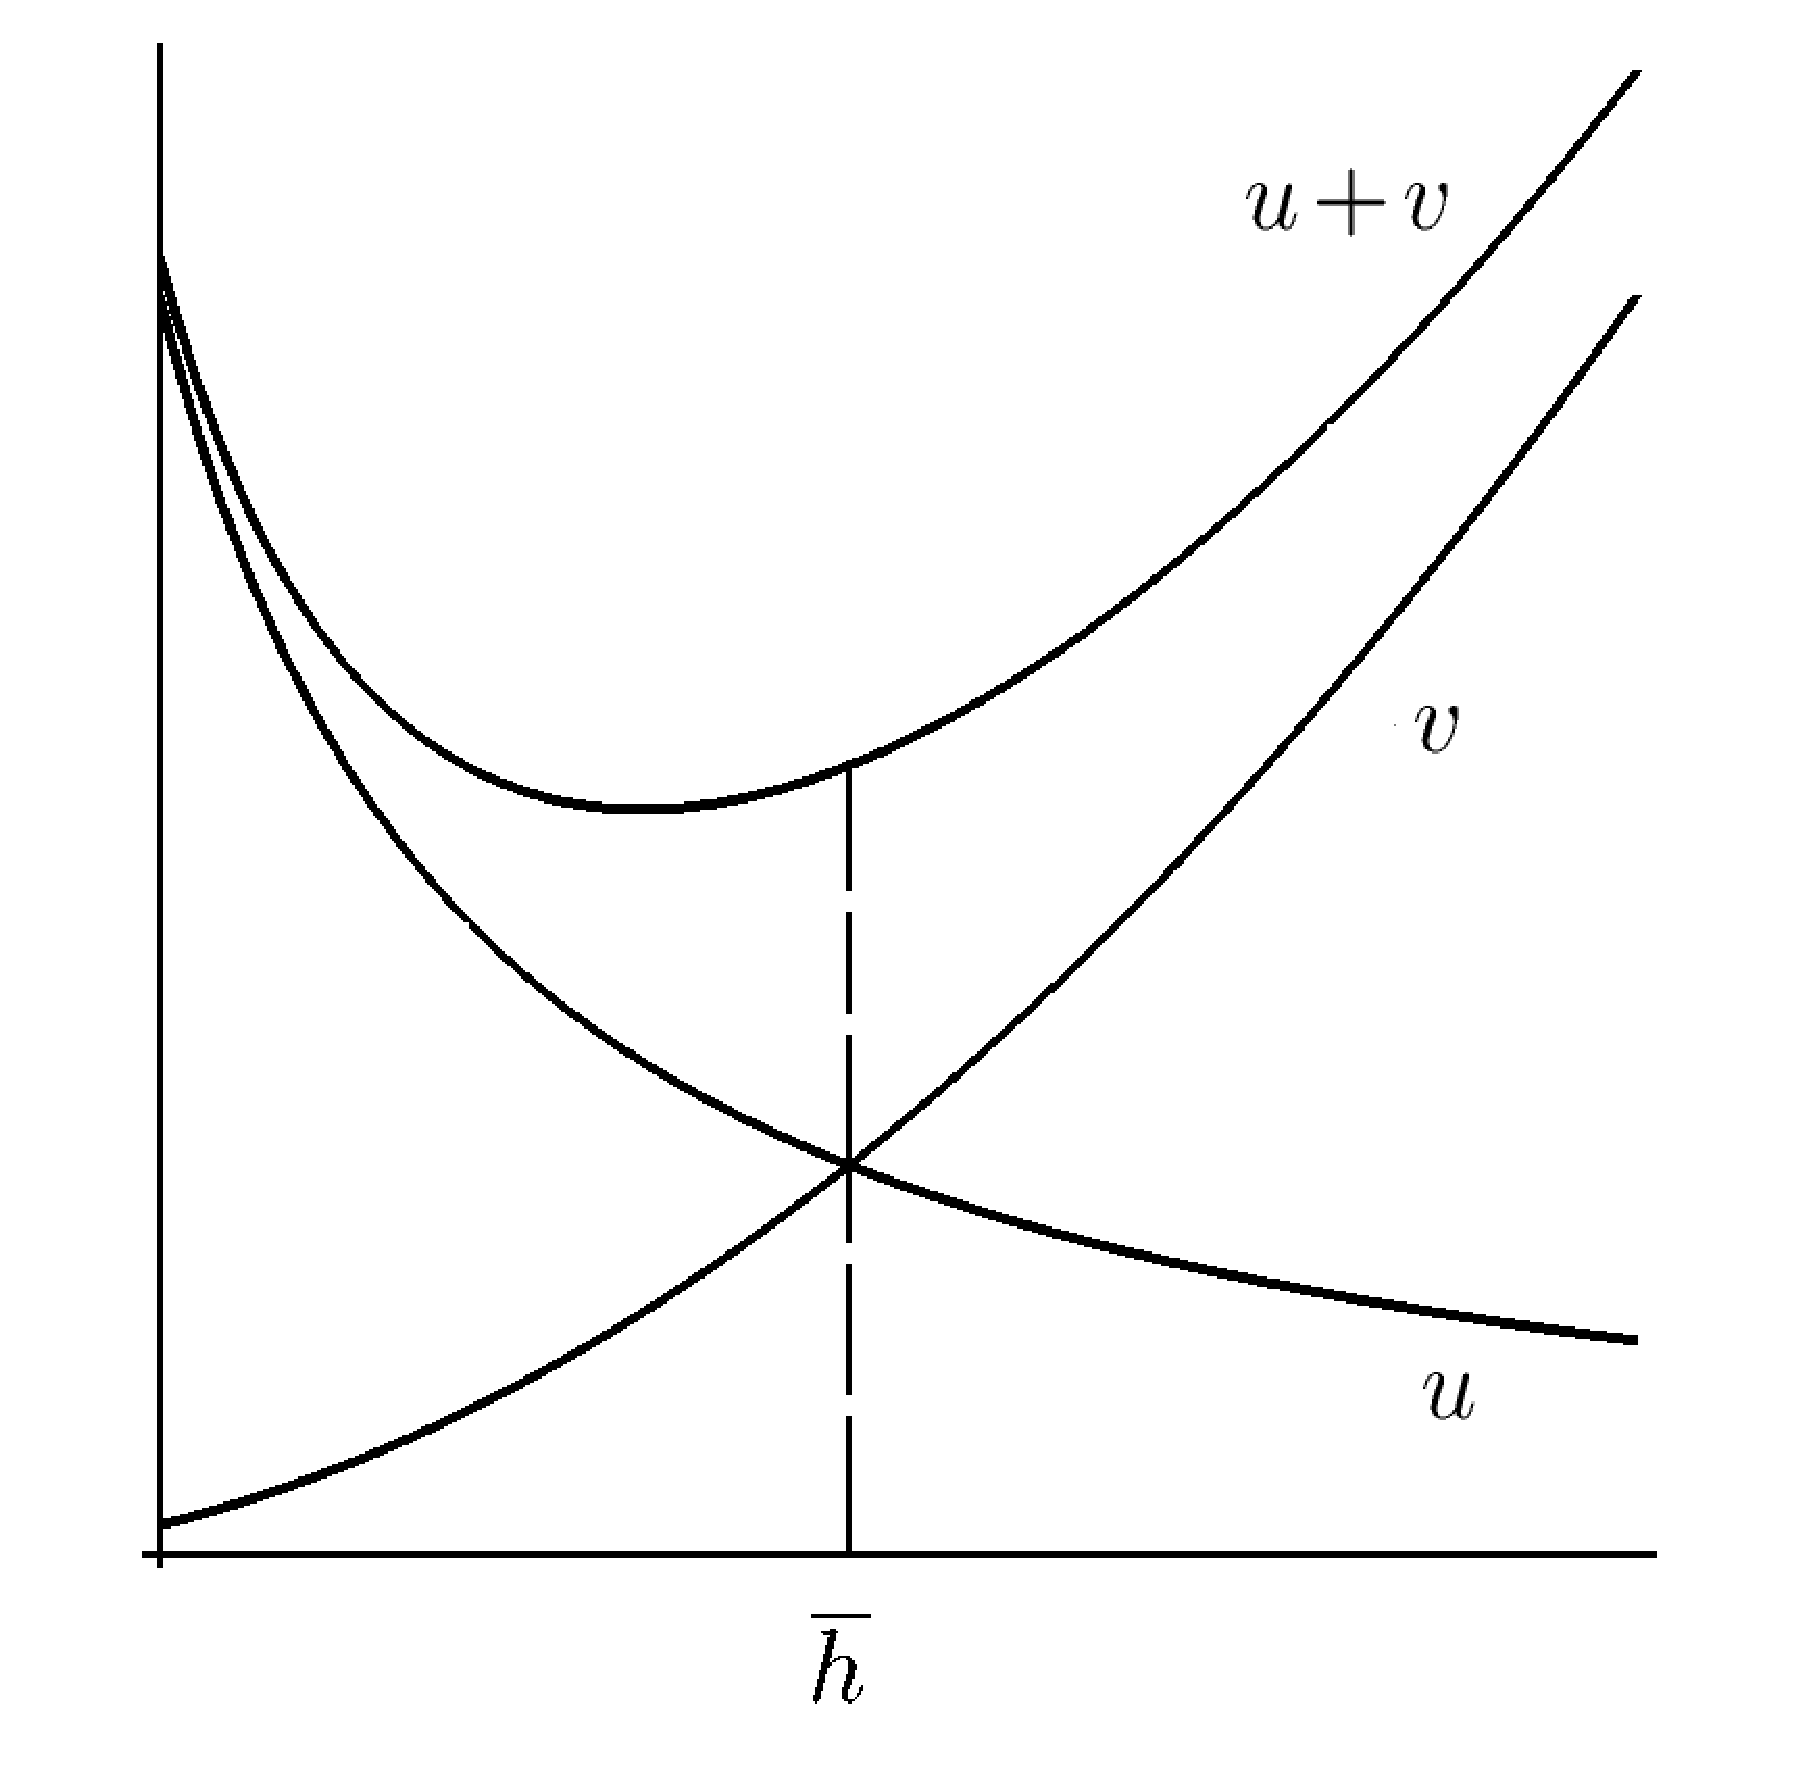
\includegraphics[width=0.4\textwidth]{pict/pict20-1.eps}
\end{center}
 \bigskip
 \refstepcounter{ris}\label{r20-1}

 \centerline{╨а╨╕╤Б.~\theris}
 \bigskip
\end{figure}


╨Т ╨┐╤А╨░╨▓╨╛╨╣ ╤З╨░╤Б╤В╨╕~(\ref{f20-4}) ╤Б╨╗╨░╨│╨░╨╡╨╝╨╛╨╡  $h^{-k}$ ╤Г╨▒╤Л╨▓╨░╨╡╤В, ╨░ $h^{l-k}$
╨▓╨╛╨╖╤А╨░╤Б╤В╨░╨╡╤В; ╨╕╤Б╤Е╨╛╨┤╤П ╨╕╨╖ ╤Б╤Д╨╛╤А╨╝╤Г╨╗╨╕╤А╨╛╨▓╨░╨╜╨╜╨╛╨│╨╛ ╨┐╤А╨╕╨╜╤Ж╨╕╨┐╨░ ╨▓╤Л╨▒╨╡╤А╨╡╨╝ ╤В╨╛╤З╨║╤Г
 $h=\overline h$ ╨╕╨╖
 ╤Г╤Б╨╗╨╛╨▓╨╕╤П $(\overline h)^{-k}\|f\|_C=(\overline h)^{l-k}\|f^{(l)}\|_C,$ ╤З╤В╨╛ ╨┤╨░╨╡╤В ╨╖╨╜╨░╤З╨╡╨╜╨╕╨╡
 $$
  \overline h=\left( \frac{\|f\|_C}{\|f^{(l)}\|_C}\right)^{\frac{1}{l}}.
 $$
 ╨Я╨╛╨┤╤Б╤В╨░╨▓╨╕╨▓ ╨╜╨░╨╣╨┤╨╡╨╜╨╜╨╛╨╡ ╨╖╨╜╨░╤З╨╡╨╜╨╕╨╡ $h$
 ╨▓~(\ref{f20-4}), ╨┐╨╛╨╗╤Г╤З╨╕╨╝ ╨╜╨╡╤А╨░╨▓╨╡╨╜╤Б╤В╨▓╨╛ ╨Ъ╨╛╨╗╨╝╨╛╨│╨╛╤А╨╛╨▓╨░
 $$
 \|f^{(k)}\|_C\le {2C_k}\|f\|_C^{\frac{l-k}{l}}\|f^{(l)}\|_C^{\frac{k}{l}}.
 $$
 ╨в╨╡╨╛╤А╨╡╨╝╨░ ╨┤╨╛╨║╨░╨╖╨░╨╜╨░ ╤Б ╨║╨╛╨╜╤Б╤В╨░╨╜╤В╨╛╨╣, ╨╜╨╡ ╨╖╨░╨▓╨╕╤Б╤П╤Й╨╡╨╣ ╨╛╤В $n:\ K_{n,k}\le \pi A_k.$

 ╨Ч\,╨░\,╨╝\,╨╡\,╤З\,╨░\,╨╜\,╨╕\,╤П.\quad
 1) ╨Э╨╡╤А╨░╨▓╨╡╨╜╤Б╤В╨▓╨╛ ╨Ъ╨╛╨╗╨╝╨╛╨│╨╛╤А╨╛╨▓╨░ ╨▓╨╡╤А╨╜╨╛   ╨╕ ╨┤╨╛╨║╨░╨╖╨░╤В╨╡╨╗╤М╤Б╤В╨▓╨╛ ╨┐╤А╨╛╤Е╨╛╨┤╨╕╤В
 ╨┤╨╗╤П ╨╗╤О╨▒╨╛╨│╨╛ ╨╛╨┤╨╜╨╛╤А╨╛╨┤╨╜╨╛╨│╨╛ ╨┐╤А╨╛╤Б╤В╤А╨░╨╜╤Б╤В╨▓╨░
 $2\pi$-╨┐╨╡╤А╨╕╨╛╨┤╨╕╤З╨╡╤Б╨║╨╕╤Е ╤Д╤Г╨╜╨║╤Ж╨╕╨╣ (╤Б╨╝. ╨╖╨░╨╝╨╡╤З╨░╨╜╨╕╨╡~\ref{r16-1}), ╤В╨░╨║ ╨║╨░╨║
 ╨╛╨▒╨╛╨▒╤Й╨╡╨╜╨╜╨╛╨╡ ╨╜╨╡╤А╨░╨▓╨╡╨╜╤Б╤В╨▓╨╛ ╨С╨╡╤А╨╜╤И╤В╨╡╨╣╨╜╨░ ╨▓╨╡╤А╨╜╨╛ ╨┤╨╗╤П ╤Н╤В╨╕╤Е
 ╨┐╤А╨╛╤Б╤В╤А╨░╨╜╤Б╤В╨▓. ╨Т ╤З╨░╤Б╤В╨╜╨╛╤Б╤В╨╕, ╨╛╨╜╨╛ ╤Б╨┐╤А╨░╨▓╨╡╨┤╨╗╨╕╨▓╨╛ ╨▓ $L_{2\pi}^p$

 2) ╨Ъ╨░╨║ ╤Г╨╢╨╡ ╨╛╤В╨╝╨╡╤З╨░╨╗╨╛╤Б╤М ╨▓ ╨╗╨╡╨║╤Ж╨╕╨╕ 19, ╨╜╨╡╤А╨░╨▓╨╡╨╜╤Б╤В╨▓╨╛~(\ref{f20-1}) ╤Б╨┐╤А╨░╨▓╨╡╨┤╨╗╨╕╨▓╨╛ ╨╕ ╨┤╨╗╤П ╤Д╤Г╨╜╨║╤Ж╨╕╨╣ ╨╜╨░ ╨▓╤Б╨╡╨╣
 ╤З╨╕╤Б╨╗╨╛╨▓╨╛╨╣ ╨┐╤А╤П╨╝╨╛╨╣.


 ╨б╨╝╤Л╤Б╨╗ ╨╜╨╡╤А╨░╨▓╨╡╨╜╤Б╤В╨▓╨░ ╨Ъ╨╛╨╗╨╝╨╛╨│╨╛╤А╨╛╨▓╨░ ╨╖╨░╨║╨╗╤О╤З╨░╨╡╤В╤Б╤П ╨▓
 ╤Б╨╗╨╡╨┤╤Г╤О╤Й╨╡╨╝: ╨╡╤Б╨╗╨╕ ╨║╨░╨║╨╛╨╝╤Г-╤В╨╛ ╨┐╤А╨╛╤Б╤В╤А╨░╨╜╤Б╤В╨▓╤Г ╨┐╤А╨╕╨╜╨░╨┤╨╗╨╡╨╢╨╕╤В
 ╤Д╤Г╨╜╨║╤Ж╨╕╤П ╨╕ ╨╡╨╡ ╤Б╤В╨░╤А╤И╨░╤П ╨┐╤А╨╛╨╕╨╖╨▓╨╛╨┤╨╜╨░╤П $f^{(l)},$
 ╤В╨╛ ╤В╨╛╨╝╤Г ╨╢╨╡ ╨┐╤А╨╛╤Б╤В╤А╨░╨╜╤Б╤В╨▓╤Г ╨┐╤А╨╕╨╜╨░╨┤╨╗╨╡╨╢╨░╤В ╨╕ ╨▓╤Б╨╡ ╨┐╤А╨╛╨╝╨╡╨╢╤Г╤В╨╛╤З╨╜╤Л╨╡
 ╨┐╤А╨╛╨╕╨╖╨▓╨╛╨┤╨╜╤Л╨╡.

 ╨Э╨╡╤А╨░╨▓╨╡╨╜╤Б╤В╨▓╨╛ ╨Ъ╨╛╨╗╨╝╨╛╨│╨╛╤А╨╛╨▓╨░ ╨╡╤Б╤В╤М ╤А╨╡╤И╨╡╨╜╨╕╨╡ ╤Б╨╗╨╡╨┤╤Г╤О╤Й╨╡╨╣
  ╨╖╨░╨┤╨░╤З╨╕. ╨Я╤Г╤Б╤В╤М  ╨╖╨░╨┤╨░╨╜╤Л ╤З╨╕╤Б╨╗╨░ $M_l\ge 0$ ╨╕ $M_0\ge 0.$
 ╨а╨░╤Б╤Б╨╝╨╛╤В╤А╨╕╨╝ ╨▓╤Б╨╡ $l$ ╤А╨░╨╖ ╨┤╨╕╤Д╤Д╨╡╤А╨╡╨╜╤Ж╨╕╤А╤Г╨╡╨╝╤Л╨╡ ╤Д╤Г╨╜╨║╤Ж╨╕╨╕ $f,$
  ╤Г ╨║╨╛╤В╨╛╤А╤Л╤Е
 $$
 \|f\|_C=M_0,\qquad \|f^{(l)}\|_C=M_l.
 $$
 ╨Ъ╨░╨║╨╛╨▓╨░ ╤В╨╛╨│╨┤╨░ ╨╛╨▒╨╗╨░╤Б╤В╤М ╨╕╨╖╨╝╨╡╨╜╨╡╨╜╨╕╤П ╨╜╨╛╤А╨╝ $\|f^{(k)}\|_C$
 ╨╕, ╨▓ ╤З╨░╤Б╤В╨╜╨╛╤Б╤В╨╕,  ╤З╨╡╨╝╤Г ╤А╨░╨▓╨╜╨╛ $M_k=\max\|f^{(k)}\|_C?$
 ╨н╤В╨░ ╨╛╨▒╨╗╨░╤Б╤В╤М ╨╛╨┐╨╕╤Б╤Л╨▓╨░╨╡╤В╤Б╤П ╨╜╨╡╤А╨░╨▓╨╡╨╜╤Б╤В╨▓╨╛╨╝ ╨Ъ╨╛╨╗╨╝╨╛╨│╨╛╤А╨╛╨▓╨░.

 \section{╨в╨╡╨╛╤А╨╡╨╝╨░ ╨╛ ╨┐╨╛╤З╨╗╨╡╨╜╨╜╨╛╨╝ ╨┤╨╕╤Д╤Д╨╡╤А╨╡╨╜╤Ж╨╕╤А╨╛╨▓╨░╨╜╨╕╨╕\\ ╤Д╤Г╨╜╨║╤Ж╨╕╨╛╨╜╨░╨╗╤М╨╜╤Л╤Е
 ╨┐╨╛╤Б╨╗╨╡╨┤╨╛╨▓╨░╤В╨╡╨╗╤М╨╜╨╛╤Б╤В╨╡╨╣}

 ╨а╨░╤Б╤Б╨╝╨╛╤В╤А╨╕╨╝ ╨╖╨░╨┤╨░╤З╤Г. ╨Я╤Г╤Б╤В╤М ╨┤╨░╨╜╨░ ╨┐╨╛╤Б╨╗╨╡╨┤╨╛╨▓╨░╤В╨╡╨╗╤М╨╜╨╛╤Б╤В╤М ╨┐╨╡╤А╨╕╨╛╨┤╨╕╤З╨╡╤Б╨║╨╕╤Е
 ╤Д╤Г╨╜╨║╤Ж╨╕╨╣ $\{f_n\}$ ╤А╨░╨▓╨╜╨╛╨╝╨╡╤А╨╜╨╛ ╤Б╤Е╨╛╨┤╤П╤Й╨░╤П╤Б╤П ╨║ ╤Д╤Г╨╜╨║╤Ж╨╕╨╕ $f$:~ $f_n\rightrightarrows
 f$ ╨╕ ╤Д╤Г╨╜╨║╤Ж╨╕╨╕ $f_n$ ╨╕╨╝╨╡╤О╤В $k$-╤Г╤О ╨┐╤А╨╛╨╕╨╖╨▓╨╛╨┤╨╜╤Г╤О.
 ╨Я╤А╨╕ ╨║╨░╨║╨╕╤Е ╤Г╤Б╨╗╨╛╨▓╨╕╤П╤Е ╨┐╤А╨╡╨┤╨╡╨╗╤М╨╜╨░╤П ╤Д╤Г╨╜╨║╤Ж╨╕╤П ╨┤╨╕╤Д╤Д╨╡╤А╨╡╨╜╤Ж╨╕╤А╤Г╨╡╨╝╨░ $k$
 ╤А╨░╨╖ ╨╕ $f_n^{(k)} \rightrightarrows f^{(k)}?$

╨Я╤А╨╡╨┤╨┐╨╛╨╗╨╛╨╢╨╕╨╝, ╨╕╨╖╨▓╨╡╤Б╤В╨╜╨╛, ╤З╤В╨╛ ╨┐╤А╨╛╨╕╨╖╨▓╨╛╨┤╨╜╤Л╨╡ ╨╜╨╡╨║╨╛╤В╨╛╤А╨╛╨│╨╛ ╨┐╨╛╤А╤П╨┤╨║╨░  $l>k$ ╤З╨╗╨╡╨╜╨╛╨▓
╨┐╨╛╤Б╨╗╨╡╨┤╨╛╨▓╨░╤В╨╡╨╗╤М╨╜╨╛╤Б╤В╨╕ ╤Б╤Г╤Й╨╡╤Б╤В╨▓╤Г╤О╤В ╨╕ ╨╛╨│╤А╨░╨╜╨╕╤З╨╡╨╜╤Л ╨╜╨╡╨║╨╛╤В╨╛╤А╨╛╨╣ ╨║╨╛╨╜╤Б╤В╨░╨╜╤В╨╛╨╣:
 $\|f_n^{(l)}\|_C\le {A},\ n\ge 1.$
 ╨Э╨░╨┐╨╕╤И╨╡╨╝ ╨╜╨╡╤А╨░╨▓╨╡╨╜╤Б╤В╨▓╨╛ ╨Ъ╨╛╨╗╨╝╨╛╨│╨╛╤А╨╛╨▓╨░ ╨┤╨╗╤П ╤А╨░╨╖╨╜╨╛╤Б╤В╨╡╨╣ $f_n-f_m$:
  $$
 \|f_n^{(k)}-f_m^{(k)}\|_C\le K \|f_n-f_m\|_C^{\frac{k}{l}}\cdot
 (2{A})^{\frac{l-k}{l}};
 $$
 ╨┐╨╛╤Б╨╗╨╡╨┤╨╜╨╡╨╡ ╨╜╨╡╤А╨░╨▓╨╡╨╜╤Б╤В╨▓╨╛ ╨┐╨╛╨║╨░╨╖╤Л╨▓╨░╨╡╤В, ╤З╤В╨╛ ╨┐╨╛╤Б╨╗╨╡╨┤╨╛╨▓╨░╤В╨╡╨╗╤М╨╜╨╛╤Б╤В╤М ╨┐╤А╨╛╨╕╨╖╨▓╨╛╨┤╨╜╤Л╤Е $\{f_n^{(k)}\}$
 ╤П╨▓╨╗╤П╨╡╤В╤Б╤П ╤Д╤Г╨╜╨┤╨░╨╝╨╡╨╜╤В╨░╨╗╤М╨╜╨╛╨╣ (╨┐╨╛╤Б╨╗╨╡╨┤╨╛╨▓╨░╤В╨╡╨╗╤М╨╜╨╛╤Б╤В╤М╤О ╨Ъ╨╛╤И╨╕) ╨╕, ╨╖╨╜╨░╤З╨╕╤В,
 ╤А╨░╨▓╨╜╨╛╨╝╨╡╤А╨╜╨╛ ╤Б╤Е╨╛╨┤╨╕╤В╤Б╤П ╨║ ╨╜╨╡╨║╨╛╤В╨╛╤А╨╛╨╣ ╤Д╤Г╨╜╨║╤Ж╨╕╨╕ $\varphi.$
 ╨Э╨╛ ╤В╨╛╨│╨┤╨░ ╨▓ ╤Б╨╕╨╗╤Г ╤Б╨╛╨╛╤В╨▓╨╡╤В╤Б╤В╨▓╤Г╤О╤Й╨╡╨╣ ╤В╨╡╨╛╤А╨╡╨╝╤Л ╨╛ ╤А╨░╨▓╨╜╨╛╨╝╨╡╤А╨╜╨╛ ╤Б╤Е╨╛╨┤╤П╤Й╨╕╤Е╤Б╤П
 ╨┐╨╛╤Б╨╗╨╡╨┤╨╛╨▓╨░╤В╨╡╨╗╤М╨╜╨╛╤Б╤В╤П╤Е ╨┤╨╕╤Д╤Д╨╡╤А╨╡╨╜╤Ж╨╕╤А╤Г╨╡╨╝╤Л╤Е ╤Д╤Г╨╜╨║╤Ж╨╕╨╣ ╨╝╨╛╨╢╨╜╨╛ ╤Г╤В╨▓╨╡╤А╨╢╨┤╨░╤В╤М,
 ╤З╤В╨╛ ╤Д╤Г╨╜╨║╤Ж╨╕╤П $f$ ╤П╨▓╨╗╤П╨╡╤В╤Б╤П $k$ ╤А╨░╨╖ ╨┤╨╕╤Д╤Д╨╡╤А╨╡╨╜╤Ж╨╕╤А╤Г╨╡╨╝╨╛╨╣ ╨╕ $\varphi=f^{(k)}$.

 ╨Ю╤В╤Б╤О╨┤╨░ ╤Б╨╗╨╡╨┤╤Г╨╡╤В, ╤З╤В╨╛ ╨╜╨░ ╨║╨╗╨░╤Б╤Б╨╡  ╤Д╤Г╨╜╨║╤Ж╨╕╨╣, $l$
 ╤А╨░╨╖ ╨┤╨╕╤Д╤Д╨╡╤А╨╡╨╜╤Ж╨╕╤А╤Г╨╡╨╝╤Л╤Е, ╤Б ╨┐╤А╨╛╨╕╨╖╨▓╨╛╨┤╨╜╨╛╨╣ ╨┐╨╛╤А╤П╨┤╨║╨░ $l,$ ╨╛╨│╤А╨░╨╜╨╕╤З╨╡╨╜╨╜╨╛╨╣ ╨╜╨╡╨║╨╛╤В╨╛╤А╨╛╨╣ ╨║╨╛╨╜╤Б╤В╨░╨╜╤В╨╛╨╣,
 ╨╛╨┐╨╡╤А╨░╤Ж╨╕╤П ╨┤╨╕╤Д╤Д╨╡╤А╨╡╨╜╤Ж╨╕╤А╨╛╨▓╨░╨╜╨╕╤П ╨┐╨╛╤А╤П╨┤╨║╨░  $k,$~ $0<k<l,$ ╨║╨╛╤А╤А╨╡╨║╤В╨╜╨░, ╨░ ╤В╨╛╤З╨╜╨╡╨╡, ╨╛╨┐╨╡╤А╨░╤В╨╛╤А
 ╨┤╨╕╤Д╤Д╨╡╤А╨╡╨╜╤Ж╨╕╤А╨╛╨▓╨░╨╜╨╕╤П ╨┐╨╛╤А╤П╨┤╨║╨░ $k$ ╨╜╨╡╨┐╤А╨╡╤А╤Л╨▓╨╡╨╜. ╨н╤В╨╛
 ╨╛╨╖╨╜╨░╤З╨░╨╡╤В, ╤З╤В╨╛ ╨╜╨░ ╤В╨░╨║╨╛╨╝ ╨║╨╗╨░╤Б╤Б╨╡ ╨╕╨╝╨╡╨╡╤В ╨╝╨╡╤Б╤В╨╛ ╤А╨╡╨│╤Г╨╗╤П╤А╨╕╨╖╨░╤Ж╨╕╤П ╨╛╨┐╨╡╤А╨░╤В╨╛╤А╨░
 ╨┤╨╕╤Д╤Д╨╡╤А╨╡╨╜╤Ж╨╕╤А╨╛╨▓╨░╨╜╨╕╤П: ╨╝╨░╨╗╨░╤П ╨╛╤И╨╕╨▒╨║╨░ ╨▓ ╨╛╨┐╤А╨╡╨┤╨╡╨╗╨╡╨╜╨╕╨╕ ╤Д╤Г╨╜╨║╤Ж╨╕╨╕ $f$
 ╨╕╨╖ ╨║╨╗╨░╤Б╤Б╨░ ╨│╨░╤А╨░╨╜╤В╨╕╤А╤Г╨╡╤В ╨╝╨░╨╗╨╛╤Б╤В╤М ╨╛╤И╨╕╨▒╨║╨╕ ╨▓╤Л╤З╨╕╤Б╨╗╨╡╨╜╨╕╤П
 ╨┐╤А╨╛╨╕╨╖╨▓╨╛╨┤╨╜╤Л╤Е $f^{(k)}\ (0<k<l)$ ╨┐╤А╨╕ ╨┐╨╛╨┤╤Е╨╛╨┤╤П╤Й╨╡╨╝ ╨╝╨╡╤В╨╛╨┤╨╡ ╨╕╤Е
 ╨▓╨╛╤Б╤Б╤В╨░╨╜╨╛╨▓╨╗╨╡╨╜╨╕╤П ╨┐╨╛ $\widetilde{f}(x) (\approx f(x)).$

 ╨Я╤Г╤Б╤В╤М $f\in {C}^{(l)}_{{2\pi}}$ ╨╕ $t_n$~--
 ╨╜╨╡╨║╨╛╤В╨╛╤А╤Л╨╣ ╤В╤А╨╕╨│╨╛╨╜╨╛╨╝╨╡╤В╤А╨╕╤З╨╡╤Б╨║╨╕╨╣ ╨┐╨╛╨╗╨╕╨╜╨╛╨╝.
 ╨Я╤А╨╕╨╝╨╡╨╜╨╕╨╝ ╨║ ╤А╨░╨╖╨╜╨╛╤Б╤В╨╕ $f-t_n$ ╨╜╨╡╤А╨░╨▓╨╡╨╜╤Б╤В╨▓╨╛ ╨Ъ╨╛╨╗╨╝╨╛╨│╨╛╤А╨╛╨▓╨░:
 $$
 \|f^{(k)}-t_n^{(k)}\|_C\le K \|f-t_n\|_C^{\frac{k}{{l}}}\cdot
 \|f^{(l)}-t_n^{(l)}\|_C^{\frac{l-k}{l}}.
 $$
 ╨Ю╤В╤Б╤О╨┤╨░ ╤Б╨╗╨╡╨┤╤Г╨╡╤В, ╤З╤В╨╛ ╨╡╤Б╨╗╨╕ ╤Д╤Г╨╜╨║╤Ж╨╕╤П ╨╕  ╨╡╨╡ ╤Б╤В╨░╤А╤И╨░╤П ╨┐╤А╨╛╨╕╨╖╨▓╨╛╨┤╨╜╨░╤П
 ╤Е╨╛╤А╨╛╤И╨╛ ╨┐╤А╨╕╨▒╨╗╨╕╨╢╨░╤О╤В╤Б╤П ╤В╤А╨╕╨│╨╛╨╜╨╛╨╝╨╡╤В╤А╨╕╤З╨╡╤Б╨║╨╕╨╝ ╨┐╨╛╨╗╨╕╨╜╨╛╨╝╨╛╨╝ ╨╕ ╨╡╨│╨╛
 {╤Б╤В╨░╤А╤И╨╡╨╣} ╨┐╤А╨╛╨╕╨╖╨▓╨╛╨┤╨╜╨╛╨╣, ╤В╨╛ ╨╕ ╨┐╤А╨╛╨╝╨╡╨╢╤Г╤В╨╛╤З╨╜╤Л╨╡ ╨┐╤А╨╛╨╕╨╖╨▓╨╛╨┤╨╜╤Л╨╡
 ╤Д╤Г╨╜╨║╤Ж╨╕╨╕ ╤В╨╛╨╢╨╡ ╤Е╨╛╤А╨╛╤И╨╛ ╨┐╤А╨╕╨▒╨╗╨╕╨╢╨░╤О╤В╤Б╤П
 {╤Б╨╛╨╛╤В╨▓╨╡╤В╤Б╤В╨▓╤Г╤О╤Й╨╕╨╝╨╕} {╨┐╤А╨╛╨╕╨╖╨▓╨╛╨┤╨╜╤Л╨╝╨╕ ╨┐╨╛╨╗╨╕╨╜╨╛╨╝╨░}.

 ╨Х╤Б╨╗╨╕ ╨▓ ╨║╨░╤З╨╡╤Б╤В╨▓╨╡ $t_n$ ╨▓╨╛╨╖╤М╨╝╨╡╨╝ ╤Б╤Г╨╝╨╝╤Л ╨д╤Г╤А╤М╨╡, ╤В╨╛ ╨┐╨╛╨╗╤Г╤З╨╕╨╝ ╨╛╤Ж╨╡╨╜╨║╤Г
 $$
   \|f^{(k)}-s_n^{(k)}\|_C\le K_{{1}} \|f-s_n \|_C^{\frac{k}{l}}\cdot
   \Big(\ln (n+1)  {E_n(f^{(l)})\Big)^{\frac{l-k}{l}},\qquad n\ge 1},
 $$
 ╨║╨╛╤В╨╛╤А╨░╤П ╨┤╨░╨╡╤В ╤Б╨▓╤П╨╖╤М ╨╝╨╡╨╢╨┤╤Г ╨┐╤А╨╕╨▒╨╗╨╕╨╢╨╡╨╜╨╕╤П╨╝╨╕ ╨┐╤А╨╛╨╕╨╖╨▓╨╛╨┤╨╜╨╛╨╣ ╨╕ ╤Д╤Г╨╜╨║╤Ж╨╕╨╕
 ╤Б╤Г╨╝╨╝╨░╨╝╨╕ ╨д╤Г╤А╤М╨╡.

 ╨Ю╤В╨╝╨╡╤В╨╕╨╝, ╤З╤В╨╛ ╨▓ ╨╜╨╡╤А╨░╨▓╨╡╨╜╤Б╤В╨▓╨╡ ╨Ъ╨╛╨╗╨╝╨╛╨│╨╛╤А╨╛╨▓╨░~(\ref{f20-1}) ╨▓ ╨┐╤А╨╛╤Б╤В╤А╨░╨╜╤Б╤В╨▓╨╡ $C_{2\pi}$
 ╨╜╨╡╨╗╤М╨╖╤П ╨╖╨░╨╝╨╡╨╜╨╕╤В╤М ╨╜╨╛╤А╨╝╤Л ╨╜╨░ ╨╜╨░╨╕╨╗╤Г╤З╤И╨╕╨╡ ╨┐╤А╨╕╨▒╨╗╨╕╨╢╨╡╨╜╨╕╤П, ╤В╨░╨║ ╨║╨░╨║ ╨▓
 ╨┐╤А╨╛╤Б╤В╤А╨░╨╜╤Б╤В╨▓╨╡ $C_{2\pi}$ ╨╜╨░╨╕╨╗╤Г╤З╤И╨╕╨╣ ╨┐╨╛╨╗╨╕╨╜╨╛╨╝ ╨┤╨╗╤П ╨┐╤А╨╛╨╕╨╖╨▓╨╛╨┤╨╜╨╛╨╣ ╨╝╨╛╨╢╨╡╤В ╨╜╨╡ ╨▒╤Л╤В╤М
 ╨┐╤А╨╛╨╕╨╖╨▓╨╛╨┤╨╜╨╛╨╣ ╨╛╤В ╨╜╨░╨╕╨╗╤Г╤З╤И╨╡╨│╨╛ ╨┐╨╛╨╗╨╕╨╜╨╛╨╝╨░ ╨┤╨╗╤П ╤Д╤Г╨╜╨║╤Ж╨╕╨╕. ╨Т $L_2$ ╤В╨░╨║╨░╤П ╨╖╨░╨╝╨╡╨╜╨░ ╨▓╨╛╨╖╨╝╨╛╨╢╨╜╨░.

╨Ш╨╝╨╡╨╡╤В╤Б╤П ╨▒╨╛╨╗╤М╤И╨╛╨╡ ╤З╨╕╤Б╨╗╨╛ ╨╕╤Б╤Б╨╗╨╡╨┤╨╛╨▓╨░╨╜╨╕╨╣, ╨┐╨╛╤Б╨▓╤П╤Й╨╡╨╜╨╜╤Л╤Е ╨▒╨╛╨╗╨╡╨╡ ╨╛╨▒╤Й╨╕╨╝
 ╨▓ ╤Б╤А╨░╨▓╨╜╨╡╨╜╨╕╨╕ ╤Б~(\ref{f20-1}) ╨╜╨╡╤А╨░╨▓╨╡╨╜╤Б╤В╨▓╨░╨╝\footnote{╨Ш╨╜╤Д╨╛╤А╨╝╨░╤Ж╨╕╤О ╨┐╨╛
 ╤Н╤В╨╛╨╣ ╤В╨╡╨╝╨░╤В╨╕╨║╨╡ ╨╝╨╛╨╢╨╜╨╛ ╨╜╨░╨╣╤В╨╕ ╨▓ ╨╛╨▒╨╖╨╛╤А╨╜╨╛╨╣ ╤А╨░╨▒╨╛╤В╨╡:
╨Р╤А╨╡╤Б╤В╨╛╨▓ ╨Т.\,╨Т. ╨Я╤А╨╕╨▒╨╗╨╕╨╢╨╡╨╜╨╕╨╡ ╨╜╨╡╨╛╨│╤А╨░╨╜╨╕╤З╨╡╨╜╨╜╤Л╤Е ╨╛╨┐╨╡╤А╨░╤В╨╛╤А╨╛╨▓ ╨╛╨│╤А╨░╨╜╨╕╤З╨╡╨╜╨╜╤Л╨╝╨╕ ╨╕
╤А╨╛╨┤╤Б╤В╨▓╨╡╨╜╨╜╤Л╨╡ ╤Н╨║╤Б╤В╤А╨╡╨╝╨░╨╗╤М╨╜╤Л╨╡ ╨╖╨░╨┤╨░╤З╨╕
 // ╨г╤Б╨┐╨╡╤Е╨╕ ╨╝╨░╤В╨╡╨╝. ╨╜╨░╤Г╨║. 1996. ╨в.\,51, ╨▓╤Л╨┐.\,6. ╨б.\,89--124.}
 $$
 \|f^{(k)}\|_{L_q}\le K\|f\|_{L_p}^{\alpha}\cdot
 \|f^{(l)}\|_{L_r}^{\beta}.
 $$


 \section{╨Э╨╡╤А╨░╨▓╨╡╨╜╤Б╤В╨▓╨╛ ╨Ф╨╢╨╡╨║╤Б╨╛╨╜╨░}

 {╨Я╤А╨╛╨╝╨╡╨╢╤Г╤В╨╛╤З╨╜╤Л╨╡ ╨┐╤А╨╕╨▒╨╗╨╕╨╢╨╡╨╜╨╕╤П (╨┐╤А╨╕╨▒╨╗╨╕╨╢╨╡╨╜╨╕╤П ╨│╨╗╨░╨┤╨║╨╕╨╝╨╕
 ╤Д╤Г╨╜╨║╤Ж╨╕╤П╨╝╨╕)}
 \vspace{3mm}

 ╨Ш╨╖╨▓╨╡╤Б╤В╨╜╨╛, ╤З╤В╨╛ ╨▓╤Б╤П╨║╤Г╤О ╨╜╨╡╨┐╤А╨╡╤А╤Л╨▓╨╜╤Г╤О ╨┐╨╡╤А╨╕╨╛╨┤╨╕╤З╨╡╤Б╨║╤Г╤О  ╤Д╤Г╨╜╨║╤Ж╨╕╤О ╨╝╨╛╨╢╨╜╨╛ ╤Б╨║╨╛╨╗╤М╨║╨╛ ╤Г╨│╨╛╨┤╨╜╨╛
 ╤В╨╛╤З╨╜╨╛ ╨┐╤А╨╕╨▒╨╗╨╕╨╖╨╕╤В╤М ╨│╨╗╨░╨┤╨║╨╕╨╝╨╕ ╤Д╤Г╨╜╨║╤Ж╨╕╤П╨╝╨╕. ╨Э╨░╨┐╤А╨╕╨╝╨╡╤А, ╤Б╤Г╨╝╨╝╨░╨╝╨╕
 ╨д╨╡╨╣╨╡╤А╨░:
 $$
 \forall\ f\in C_{{2\pi}}\qquad \forall\ \varepsilon>0\qquad \exists\ n:\qquad
 \|f-\sigma_n{(f)}\|_C<\varepsilon.
 $$
 ╨Ч╨░╨┤╨░╨┤╨╕╨╝ ╨╜╨╛╤А╨╝╨╕╤А╨╛╨▓╨╛╤З╨╜╤Л╨╡ ╨┐╨░╤А╨░╨╝╨╡╤В╤А╤Л. ╨Я╤Г╤Б╤В╤М $l$
 -- ╨╜╨░╤В╤Г╤А╨░╨╗╤М╨╜╨╛╨╡ ╤З╨╕╤Б╨╗╨╛ ╨╕ $M>0.$ ╨а╨░╤Б╤Б╨╝╨╛╤В╤А╨╕╨╝ ╨║╨╗╨░╤Б╤Б $C^{(l)}(M)$ ╨▓╤Б╨╡╤Е
 $l$ ╤А╨░╨╖ ╨╜╨╡╨┐╤А╨╡╤А╤Л╨▓╨╜╨╛ ╨┤╨╕╤Д╤Д╨╡╤А╨╡╨╜╤Ж╨╕╤А╤Г╨╡╨╝╤Л╤Е $2\pi$-╨┐╨╡╤А╨╕╨╛╨┤╨╕╤З╨╡╤Б╨║╨╕╤Е
 ╤Д╤Г╨╜╨║╤Ж╨╕╨╣ $\varphi,$ ╤Г ╨║╨╛╤В╨╛╤А╤Л╤Е  $\|\varphi^{(l)}\|_C\le M.$
 ╨Ъ╨╗╨░╤Б╤Б╨╛╨╝ $C^{(l)}(M)$ ($M$ -- ╤Д╨╕╨║╤Б╨╕╤А╨╛╨▓╨░╨╜╨╛) ╤Г╨╢╨╡ ╨╜╨╡╨╗╤М╨╖╤П  ╤Б╨║╨╛╨╗╤М ╤Г╨│╨╛╨┤╨╜╨╛ ╤В╨╛╤З╨╜╨╛
 ╨┐╤А╨╕╨▒╨╗╨╕╨╖╨╕╤В╤М ╨┐╤А╨╛╨╕╨╖╨▓╨╛╨╗╤М╨╜╤Г╤О
 ╤Д╤Г╨╜╨║╤Ж╨╕╤О. ╨Т╨╛╨╖╨╜╨╕╨║╨░╨╡╤В ╤Б╨╗╨╡╨┤╤Г╤О╤Й╨░╤П ╨┐╤А╨╛╨▒╨╗╨╡╨╝╨░.

 \task %%% ╨Ч╨░╨┤╨░╤З╨░.
 ╨Э╨░╨╣╤В╨╕
 $$
 \inf_{\varphi\in C^{(l)}(M)} \|f-\varphi\|_C=E(f,C^{(l)}(M)).
 $$
 ╨н╤В╨░ ╨╖╨░╨┤╨░╤З╨░ ╨▒╨╡╤Б╨║╨╛╨╜╨╡╤З╨╜╨╛╨╝╨╡╤А╨╜╨░╤П ╨╕ ╨╜╨╡╨╗╨╕╨╜╨╡╨╣╨╜╨░╤П.

\vspace{3mm}
 {\bf 1. ╨Ю ╤Б╨│╨╗╨░╨╢╨╕╨▓╨░╨╜╨╕╨╕ ╤Д╤Г╨╜╨║╤Ж╨╕╨╣}
 \vspace{3mm}

 ╨Я╤А╨╕ $l=1,2$ ╨║╨╗╨░╤Б╤Б╨╕╤З╨╡╤Б╨║╨╛╨╡ ╤А╨╡╤И╨╡╨╜╨╕╨╡ ╨╖╨░╨┤╨░╤З╨╕ ╨╛ ╤Б╨│╨╗╨░╨╢╨╕╨▓╨░╨╜╨╕╨╕ ╨┤╨░╨╡╤В╤Б╤П
 ╤Б ╨┐╨╛╨╝╨╛╤Й╤М╤О ╨╛╨┐╤А╨╡╨┤╨╡╨╗╤П╨╡╨╝╤Л╤Е ╨╜╨╕╨╢╨╡ ╤Д╤Г╨╜╨║╤Ж╨╕╨╣ ╨б╤В╨╡╨║╨╗╨╛╨▓╨░.

 ╨Я╤Г╤Б╤В╤М $h>0;$ ╤Г╤Б╤А╨╡╨┤╨╜╨╕╨╝ ╤Д╤Г╨╜╨║╤Ж╨╕╤О $f{\in C_{2\pi}}$ ╨┐╨╛ ╨╛╤В╤А╨╡╨╖╨║╤Г
 ╨┤╨╗╨╕╨╜╤Л $h$ ╤Б ╤Ж╨╡╨╜╤В╤А╨╛╨╝ ╨▓ ╤В╨╛╤З╨║╨╡ $x.$  ╨Т ╤А╨╡╨╖╤Г╨╗╤М╤В╨░╤В╨╡ ╨┐╨╛╨╗╤Г╤З╨╕╨╝ ╤Д╤Г╨╜╨║╤Ж╨╕╤О
    \begin{equation}\label{f20-VAS-1}
  f_h(x)=\frac{1}{h}
 \int_{-\frac{h}{2}}^{\frac{h}{2}} f(x+t)\, dt,
\end{equation}
 ╨║╨╛╤В╨╛╤А╨░╤П ╨╜╨░╨╖╤Л╨▓╨░╨╡╤В╤Б╤П  ╤Д╤Г╨╜╨║╤Ж╨╕╨╡╨╣ ╨б╤В╨╡╨║╨╗╨╛╨▓╨░. ╨б╨│╨╗╨░╨╢╨╡╨╜╨╜╨░╤П ╤Д╤Г╨╜╨║╤Ж╨╕╤П~(\ref{f20-VAS-1})
 ╤Г╨╢╨╡ ╨╜╨╡╨┐╤А╨╡╤А╤Л╨▓╨╜╨╛ ╨┤╨╕╤Д╤Д╨╡╤А╨╡╨╜╤Ж╨╕╤А╤Г╨╡╨╝╨░ ╨╕
 $$
 f_h'(x)=\frac{1}{h} \left\{ f\left( x+\frac{h}{2}\right)-f\left(
 x-\frac{h}{2}\right)\right\}.
 $$
 ╨б╨┐╤А╨░╨▓╨╡╨┤╨╗╨╕╨▓╤Л ╤Б╨╗╨╡╨┤╤Г╤О╤Й╨╕╨╡ ╤Б╨╛╨╛╤В╨╜╨╛╤И╨╡╨╜╨╕╤П:
 $$
 \|f_h'\|_C\le \frac{2}{h}\|f\|_C,
 $$
 $$
 \|f-f_h\|_C\le \frac{1}{h}
 \int_{-\frac{{h}}{2}}^{\frac{{h}}{2}} \| f(x)-f(x+t)\|_C\, dt\le
 \frac{2}{h}
 \int_{0}^{\frac{h}{2}} \omega(f,t)\, dt\le \omega\left(
 f,\frac{h}{2}\right).
 $$
 ╨б╨╗╨╡╨┤╨╛╨▓╨░╤В╨╡╨╗╤М╨╜╨╛, ╤Д╤Г╨╜╨║╤Ж╨╕╤П ╨б╤В╨╡╨║╨╗╨╛╨▓╨░ ╨┐╤А╨╕╨▒╨╗╨╕╨╢╨░╨╡╤В ╨╕╤Б╤Е╨╛╨┤╨╜╤Г╤О ╤Д╤Г╨╜╨║╤Ж╨╕╤О ╨╕ ╤П╨▓╨╗╤П╨╡╤В╤Б╤П ╨╜╨╡╨┐╤А╨╡╤А╤Л╨▓╨╜╨╛
 ╨┤╨╕╤Д╤Д╨╡╤А╨╡╨╜╤Ж╨╕╤А╤Г╨╡╨╝╨╛╨╣. ╨Ю╨┤╨╜╨░╨║╨╛, ╨┐╤А╨╕ ╤Е╨╛╤А╨╛╤И╨╡╨╝ ╨┐╤А╨╕╨▒╨╗╨╕╨╢╨╡╨╜╨╕╨╕ ╨┐╤А╨╛╨╕╨╖╨▓╨╛╨┤╨╜╨░╤П $f'_h,$ ╨▓╨╛╨╛╨▒╤Й╨╡ ╨│╨╛╨▓╨╛╤А╤П,
 ╨▒╤Г╨┤╨╡╤В ╨▒╨╛╨╗╤М╤И╨╛╨╣.

 ╨Я╨╛ ╨▓╨╡╤Й╨╡╤Б╤В╨▓╨╡╨╜╨╜╨╛╨╝╤Г ╤З╨╕╤Б╨╗╤Г $M>0$ ╨▓╤Л╨▒╨╡╤А╨╡╨╝ ╨┐╨░╤А╨░╨╝╨╡╤В╤А $h$ ╤В╨░╨║, ╤З╤В╨╛╨▒╤Л $M=\dfrac{2}{h}\|f\|_C,$
 ╤В.\,╨╡. ╨▓╨╛╨╖╤М╨╝╨╡╨╝ $h=\dfrac{2\|f\|_C}{M}.$ ╨Т ╤А╨╡╨╖╤Г╨╗╤М╤В╨░╤В╨╡ ╨┐╤А╨╕╤Е╨╛╨┤╨╕╨╝ ╨║ ╤Б╨╗╨╡╨┤╤Г╤О╤Й╨╡╨╝╤Г ╤Г╤В╨▓╨╡╤А╨╢╨┤╨╡╨╜╨╕╤О ╨╛ ╨┐╤А╨╕╨▒╨╗╨╕╨╢╨╡╨╜╨╕╨╕ ╤Д╤Г╨╜╨║╤Ж╨╕╤П╨╝╨╕ ╨б╤В╨╡╨║╨╗╨╛╨▓╨░.

 \begin{teo} ╨Ф╨╗╤П ╨║╨░╨╢╨┤╨╛╨╣ ╤Д╤Г╨╜╨║╤Ж╨╕╨╕ $f\in C_{{2\pi}}$ ╨╕ ╨╗╤О╨▒╨╛╨╣ ╨║╨╛╨╜╤Б╤В╨░╨╜╤В╤Л $M>0$ ╤Б╤Г╤Й╨╡╤Б╤В╨▓╤Г╨╡╤В
 ╨╜╨╡╨┐╤А╨╡╤А╤Л╨▓╨╜╨╛ ╨┤╨╕╤Д╤Д╨╡╤А╨╡╨╜╤Ж╨╕╤А╤Г╨╡╨╝╨░╤П ╤Д╤Г╨╜╨║╤Ж╨╕╤П $\varphi$ ╤Б╨╛ ╤Б╨▓╨╛╨╣╤Б╤В╨▓╨╛╨╝
 $\|\varphi'\|_C\le M$ ╤В╨░╨║╨░╤П,~╤З╤В╨╛
 $$
  \|f-\varphi\|_C\le \omega\left( f,\frac{\|f\|_C}{M}\right).
 $$
 \end{teo}

 ╨Р╨╜╨░╨╗╨╛╨│╨╕╤З╨╜╨╛ ╨╕╤Б╤Б╨╗╨╡╨┤╤Г╨╡╤В╤Б╤П ╤Б╨╗╤Г╤З╨░╨╣ $l=2.$
╨а╨░╤Б╤Б╨╝╨╛╤В╤А╨╕╨╝ ╨▓╤В╨╛╤А╤Г╤О ╤А╨░╨╖╨╜╨╛╤Б╤В╤М
   $$
 \Delta_t^2 f(x)=f(x+t)-2f(x)+f(x-t).
 $$
 ╨Я╤А╨╛╨╕╨╜╤В╨╡╨│╤А╨╕╤А╨╛╨▓╨░╨▓ 2 ╤А╨░╨╖╨░, ╨┐╨╛╨╗╤Г╤З╨╕╨╝ ╤Б╨╛╨╛╤В╨╜╨╛╤И╨╡╨╜╨╕╨╡
  \begin{equation}\label{f20-5}
 \frac{1}{h^2}\int_0^{h}\int_0^{t_1} \Delta_t^2 f(x)\, dt\
 dt_1=\varphi(x)-f(x),
 \end{equation}
 ╨▓ ╨║╨╛╤В╨╛╤А╨╛╨╝
  \begin{equation}\label{f20-5a}
 \varphi(x)=\frac{1}{h^2}\int_0^{h}\int_0^{t_1} (f(x+t)+f(x-t))\, dt\
 dt_1.
  \end{equation}
 ╨б╨┤╨╡╨╗╨░╨▓ ╨▓ ╨╛╨┤╨╜╨╛╨╝ ╨╕╨╜╤В╨╡╨│╤А╨░╨╗╨╡ ╨╖╨░╨╝╨╡╨╜╤Г ╨┐╨╡╤А╨╡╨╝╨╡╨╜╨╜╨╛╨│╨╛ $x+t=u,$ ╨░ ╨▓╨╛ ╨▓╤В╨╛╤А╨╛╨╝ $x-t=u,$ ╨┐╨╛╨╗╤Г╤З╨░╨╡╨╝ ╨┐╤А╨╡╨┤╤Б╤В╨░╨▓╨╗╨╡╨╜╨╕╨╡
 $$
 \varphi(x)=\frac{1}{h^2}\int_0^{h}\int_{x-t_1}^{x+t_1} f(u)\ du\  dt_1.
 $$
 ╨н╤В╨░ ╤Д╤Г╨╜╨║╤Ж╨╕╤П ╨┤╨╕╤Д╤Д╨╡╤А╨╡╨╜╤Ж╨╕╤А╤Г╨╡╨╝╨░ ╨┐╨╛ $x$ ╨╕
 $$
 \varphi'(x)=\frac{1}{h^2}\int_0^{h}(f(x+t_1)-f(x-t_1))\  dt_1=\frac{1}{h^2}\left(\int_x^{x+h}f(v)\ dv-\int_{x-h}^{x}f(v)\ dv\right).
 $$
╨Я╨╛╤Б╨╗╨╡╨┤╨╜╨╡╨╡ ╨▓╤Л╤А╨░╨╢╨╡╨╜╨╕╨╡ ╨▓╨╜╨╛╨▓╤М ╨┤╨╕╤Д╤Д╨╡╤А╨╡╨╜╤Ж╨╕╤А╤Г╨╡╨╝╨╛, ╨░, ╨╖╨╜╨░╤З╨╕╤В, ╤Д╤Г╨╜╨║╤Ж╨╕╤П $\varphi$ ╨┤╨▓╨░╨╢╨┤╤Л
╨┤╨╕╤Д╤Д╨╡╤А╨╡╨╜╤Ж╨╕╤А╤Г╨╡╨╝╨░ ╨╕
 \begin{equation}\label{f20-6}
 \varphi''(x)=\frac{1}{h^2}\left(f(x+h)-2f(x)+f(x-h)\right).
\end{equation}

╨б╨╗╨╡╨┤╨╛╨▓╨░╤В╨╡╨╗╤М╨╜╨╛, ╤Д╤Г╨╜╨║╤Ж╨╕╤П $\varphi$ ╨┤╨▓╨░╨╢╨┤╤Л ╨╜╨╡╨┐╤А╨╡╤А╤Л╨▓╨╜╨╛ ╨┤╨╕╤Д╤Д╨╡╤А╨╡╨╜╤Ж╨╕╤А╤Г╨╡╨╝╨░ ╨╕, ╨║╨░╨║ ╨╜╨╡╤В╤А╤Г╨┤╨╜╨╛
╤Г╨▓╨╕╨┤╨╡╤В╤М ╨╕╨╖~(\ref{f20-6}) ╨╕~(\ref{f20-5}), ╨╛╨▒╨╗╨░╨┤╨░╨╡╤В ╤Б╨╗╨╡╨┤╤Г╤О╤Й╨╕╨╝╨╕ ╤Б╨▓╨╛╨╣╤Б╤В╨▓╨░╨╝╨╕:
 \begin{equation}\label{f20-7}
 \|\varphi''\|_C\le \frac{1}{h^2} \|\Delta_h^2 f\|_C\le\frac{4}{h^2}\,\|f\|_C,\qquad
 \|f-\varphi\|_C\le \frac{1}{2}\,\omega_2(h,f).
 \end{equation}

 \vspace{3mm}
 {\bf 2. ╨Э╨╡╤А╨░╨▓╨╡╨╜╤Б╤В╨▓╨╛ ╨Ф╨╢╨╡╨║╤Б╨╛╨╜╨░ ╨▓ ${C_{2\pi}}$}
 \vspace{3mm}

 ╨Я╤А╨╛╤Ж╨╡╨┤╤Г╤А╨░ ╤Б╨│╨╗╨░╨╢╨╕╨▓╨░╨╜╨╕╤П  ╨╕ ╨╜╨╡╤А╨░╨▓╨╡╨╜╤Б╤В╨▓╨╛ ╨д╨░╨▓╨░╤А╨░ ╨┐╨╛╨╖╨▓╨╛╨╗╤П╤О╤В
 ╨╛╤Ж╨╡╨╜╨╕╤В╤М ╨┐╤А╨╕╨▒╨╗╨╕╨╢╨╡╨╜╨╕╨╡ ╨┐╤А╨╛╨╕╨╖╨▓╨╛╨╗╤М╨╜╨╛╨╣ ╤Д╤Г╨╜╨║╤Ж╨╕╨╕ ╤З╨╡╤А╨╡╨╖ ╤Е╨░╤А╨░╨║╤В╨╡╤А╨╕╤Б╤В╨╕╨║╨╕ ╨╡╨╡ ╨│╨╗╨░╨┤╨║╨╛╤Б╤В╨╕.

 \begin{teo}[╨Ф.\,╨Ф╨╢╨╡╨║╤Б╨╛╨╜]
 ╨Я╤А╨╕ ╨╗╤О╨▒╨╛╨╝ $k\ge 0$ ╤Б╤Г╤Й╨╡╤Б╤В╨▓╤Г╨╡╤В ╨║╨╛╨╜╤Б╤В╨░╨╜╤В╨░ $C_k$ ╤В╨░╨║╨░╤П, ╤З╤В╨╛ ╨┤╨╗╤П ╤Д╤Г╨╜╨║╤Ж╨╕╨╣
 $f\in {C}^{(k)}$ ╤Б╨┐╤А╨░╨▓╨╡╨┤╨╗╨╕╨▓╨╛ ╨╜╨╡╤А╨░╨▓╨╡╨╜╤Б╤В╨▓╨╛
  $$
 E_n(f)_C\le \frac{C_k}{(n+1)^k}\, \omega_2\left(
 \frac{1}{n},f^{(k)}\right).
 $$
 \end{teo}

 \begin{proof} %%% ╨Ф╨╛╨║╨░╨╖╨░╤В╨╡╨╗╤М╤Б╤В╨▓╨╛.
 ╨Я╨╛ ╨╜╨╡╤А╨░╨▓╨╡╨╜╤Б╤В╨▓╤Г ╨д╨░╨▓╨░╤А╨░~(\ref{f19-5})
 $$
 E_n(f)_C\le \frac{M_k}{(n+1)^k} E_n(f^{(k)})_C;
 $$
 ╤В╨╡╨┐╨╡╤А╤М ╨┤╨╛╤Б╤В╨░╤В╨╛╤З╨╜╨╛ ╨╛╤Ж╨╡╨╜╨╕╤В╤М $E_n(f^{(k)})_C.$ ╨Я╨╛╤Б╤В╤А╨╛╨╕╨╝  ╤Д╤Г╨╜╨║╤Ж╨╕╤О   $\varphi$  (╤Б╨╝.~(\ref{f20-5a}))
 ╨┤╨╗╤П ╨┐╤А╨╛╨╕╨╖╨▓╨╛╨┤╨╜╨╛╨╣ $f^{(k)}$ ╤Б╨╛ ╨╖╨╜╨░╤З╨╡╨╜╨╕╨╡╨╝ ╨┐╨░╤А╨░╨╝╨╡╤В╤А╨░  $h=\dfrac{1}{n}.$
 ╨в╨╛╨│╨┤╨░  ╨▓ ╤Б╨╕╨╗╤Г~(\ref{f20-7}) ╨▒╤Г╨┤╨╡╨╝ ╨╕╨╝╨╡╤В╤М
 $$
 \|\varphi''\|_C\le  n^2
 \left\| \Delta_{\frac{1}{n}}^2 f^{(k)}\right\|_C\le
  n^2\omega_2\left( \frac{1}{n},f^{(k)}\right)
 $$
 ╨╕, ╤Б╨╗╨╡╨┤╨╛╨▓╨░╤В╨╡╨╗╤М╨╜╨╛, ╨┐╨╛ ╨╜╨╡╤А╨░╨▓╨╡╨╜╤Б╤В╨▓╤Г ╨д╨░╨▓╨░╤А╨░
 $$
 E_n(\varphi)_C\le \frac{M_2}{(n+1)^2} n^2\omega_2
 \left( \frac{1}{n},f^{(k)}\right).
 $$
 ╨Я╨╛╤Б╨║╨╛╨╗╤М╨║╤Г
 $$
 E_n(f^{(k)})_C\le E_n(f^{(k)}-\varphi)_C+E_n(\varphi)_C\le \|f^{(k)}-\varphi\|_C+E_n(\varphi)_C,
 $$
 ╤В╨╛ (╨▓╨╜╨╛╨▓╤М ╤Б ╨┐╨╛╨╝╨╛╤Й╤М╤О~(\ref{f20-7})) ╨┐╤А╨╕╤Е╨╛╨┤╨╕╨╝ ╨║ ╨╛╤Ж╨╡╨╜╨║╨╡
  $$
 E_n(f^{(k)})_C\le \left(\frac{1}{2}+M_2\right) \omega_2
 \left( \frac{1}{n},f^{(k)}\right).
 $$
 ╨в╨╡╨╛╤А╨╡╨╝╨░ ╨┤╨╛╨║╨░╨╖╨░╨╜╨░.
 \end{proof}

 ╨Я╤А╨╕ $k=0$ ╨┐╨╛╨╗╤Г╤З╨░╨╡╨╝   ╨╜╨╡╤А╨░╨▓╨╡╨╜╤Б╤В╨▓╨╛ ╨Ф╨╢╨╡╨║╤Б╨╛╨╜╨░ ╨┤╨╗╤П ╨╜╨╡╨┤╨╕╤Д╤Д╨╡╤А╨╡╨╜╤Ж╨╕╤А╤Г╨╡╨╝╤Л╤Е ╤Д╤Г╨╜╨║╤Ж╨╕╨╣
 $$
 E_n(f)_C\le C\omega_2\left( \frac{1}{n},f\right).
 $$

 \begin{Remark} %%% ╨Ч╨░╨╝╨╡╤З╨░╨╜╨╕╨╡.
 ╨н╤В╨╛ ╨┤╨╛╨║╨░╨╖╨░╤В╨╡╨╗╤М╤Б╤В╨▓╨╛ ╤В╨╡╨╛╤А╨╡╨╝╤Л ╨Ф╨╢╨╡╨║╤Б╨╛╨╜╨░ ╨┐╤А╨╛╤Е╨╛╨┤╨╕╤В ╨▓ ╨╗╤О╨▒╨╛╨╝ ╨╛╨┤╨╜╨╛╤А╨╛╨┤╨╜╨╛╨╝ ╨┐╤А╨╛╤Б╤В╤А╨░╨╜╤Б╤В╨▓╨╡.
 \end{Remark}


 \newpage
\thispagestyle{empty}
\normalsize
\begin{center}
НАУЧНОЕ ИЗДАНИЕ\\[24pt]
{\large\textbf{Изложение лекций С.\,Б.\,Стечкина по теории приближений}}\\[4pt]


\vspace{28pt}

Рекомендовано к изданию\\
ученым советом\\
Института математики и механики\\
и НИСО\ УрО\ РАН
\end{center}

\vspace{5pt}

%\bc
%ЛР \No\,020764  от  24.04.98. \\
%\ec

%\vfill


%\bc
%    Редактор~{\em{?.\,?.\,???}}
%\ec
%\vfill
\begin{center}
% Оригинал-макет подготовлен в РИО ИММ УрО РАН\\[2pt]

    Редактор~{\em{Е.\,Е.\,Понизовкина}}\\[2ex]

 Компьютерная верстка: {\em{А.\,И.\,Козко, Ю.\,В.\,Малыхин,
М.\,В.\,Дейкалова, В.\,В.\,Шевченко}}\\[1ex]
% Отв. за выпуск {\em{Н.\,В.\,Маслова}}

\end{center}
\vfill

\hrule

%\bigskip
\begin{center}  \footnotesize \noindent НИСО УрО РАН\,\ \No~..(..)--...\\
Подписано в печать~20.07.10. Формат ...$\times$.../...\linebreak
Печать офсетная.\ Усл.печ.л.~...\ Уч.-изд.л.~...\
Тираж~500.\linebreak %Заказ~2374
\hrule
\end{center}

%\bigskip
\begin{center}
\footnotesize
 Оригинал-макет подготовлен в ИММ УрО РАН\\[2pt]
\end{center}

\begin{center}
\footnotesize
%Институт математики и механики УрО РАН\\
     620990 г.~Екатеринбург,
     ул.\ С.~Ковалевской, 16.\\ [2ex]

Отпечатано с готовых диапозитивов в типографии \\ ООО
``Издательство Учебно-методический центр --- УПИ''\\ 620002 г.
Екатеринбург, ул.  Мира, 17.

\end{center}


\end{document}
